\documentclass[table,xcdraw]{report}


%\usepackage{gentium}
\usepackage{fontspec}
\usepackage{float}
\usepackage[xetex]{graphicx} % Required for including pictures
\usepackage[xetex,linkcolor=black,pdfborder={0 0 0}]{hyperref} % Format links for pdf
\usepackage{calc} % To reset the counter in the document after title page
\usepackage{enumitem} % Includes lists
\usepackage{longtable}
\usepackage{chngpage}
\usepackage{tocbasic}

\frenchspacing % No double spacing between sentences
\linespread{1.5} % Set linespace
\usepackage[a4paper, lmargin=0.1666\paperwidth, rmargin=0.1666\paperwidth, tmargin=0.1111\paperheight, bmargin=0.1111\paperheight]{geometry} %margins
%\usepackage{parskip}

\usepackage[all]{nowidow} % Tries to remove widows

\usepackage{todonotes}
\usepackage{lipsum} % Used for inserting dummy 'Lorem ipsum' text into the template
\usepackage{verbatim}
\usepackage{csquotes}
\usepackage{polyglossia}
\usepackage{multirow}
\usepackage{caption}
\usepackage{longtable}
\usepackage{multicol}
\captionsetup[table]{labelfont=sc,textfont=it,font=small,justification=centering}
\setdefaultlanguage{english}
\setotherlanguages{tibetan}
\setmainfont{Libertinus Serif}
\newfontfamily\tibetanfont{Microsoft Himalaya}
\usepackage[backend=biber,style=unified,maxcitenames=2,maxbibnames=99]{biblatex}
\usepackage{amsmath}
\usepackage{adjustbox}

\usepackage[edges,linguistics]{forest}
\usepackage{rotating}

\newcounter{Appendix}
\newcounter{Figure}
\bibliography{sources}
\let \citeNP \cite
\let \citeA \textcite
\let \cite \parencite
\let \citesNP \cites
\let \cites \parencites
\let \citesA \textcites
\let \sc \textsc
\DeclareNewTOC[%
  type=map,
  float,
  name=Map,
  listname={List of Maps},
  ]{map}
\makeatletter
  \renewcommand\l@map{\l@figure}
\makeatother
\graphicspath{{./figures/}}

\forestset{
  phylogeny/.style={
    where n children=0{
      tier=word
    }{},
    nice empty nodes, forked edges, for tree={l=10mm,l sep=10mm, calign=midpoint}
  }
}

\title{A Typological Survey of Addressee-perspective in Trans-Himalayan Languages}
\author{Carl Bodnaruk}
\date{April 2024}
\newcommand{\lfam}{Trans-Himalayan}
\newcommand{\lfamreason}{in order to avoid giving any undue authority to any particular language or political entity, and to avoid the inevitable confusion between `Tibeto-Burman' as the whole family and `Tibeto-Burman' as the non-Sinitic branch of `Sino-Tibetan'.}
\newcommand{\tibetnat}{People's Republic of China}
    \newcommand{\figref}[1]{\figurename~\ref{#1}}
    \newcommand{\appref}[1]{Appendix \ref{#1}}
    \newcommand{\tabref}[1]{Table \ref{#1}}
    \newcommand{\exref}[1]{(\ref{#1})}
    \newcommand{\mapref}[1]{Map \ref{#1}}
    \newcommand{\sref}[1]{Section \ref{#1}}
    \newcommand{\cref}[1]{Chapter \ref{#1}}
    \let\eachwordone=\it
    \setcounter{secnumdepth}{3}
\usepackage{gb4e}

\let\eachwordone=\it

\begin{document}
\maketitle

\tableofcontents
\chapter{Introduction}\label{c:Introduction}
\section{Overview of this thesis}
The study of cross-linguistic functional categories such as evidentiality, egophoricity, epistemic modality, engagement, and mirativity is a growing field in linguistics, seeing a huge rise in number of publications. over the forty years since \citeA{ChafeNichols1986} made a case for evidentiality as a cross-linguistic category. This thesis provides a typological overview of these categories within the \lfam\ language family, a language family showing widespread epistemic marking and home to many of the languages which informed our early understanding of these categories. It uses published data and analyses of epistemic marking in 67 \lfam\ languages\footnote{A full list is given in \appref{a:TableOfLanguages}} and original data and analysis of one language to draw up an initial typological description of this marking in the family. This foundation is then used to establish some broader theoretical conclusions about epistemic marking in the \lfam\ family and cross-linguistically. It argues for a cross-linguistically valid supercategory of epistemic marking (introduced in \ref{s:Intro:Thesis} below) linking these traditionally similar-but-separate functional categories visible throughout the \lfam\ family both functionally and formally, and presents this category of epistemic marking as better able to account for some features of these grammatical systems described in \lfam\ languages.

This thesis is divided into seven chapters. This first chapter provides an overview of the thesis and its argument, as well as an overview of the literature on important and relevant concepts such as epistemic marking, intersubjectivity, and perspective in language. Chapter \ref{c:THOverview} gives an in-depth introduction to the \lfam\ language family, including an overview of the family, the current state of research and description, and the history of linguistic research in the area. Chapter \ref{c:Methods} details the development of a database of summarised descriptions of \lfam\ languages in terms of the selection of languages and data and its representation in an accessible and comparable format. Chapter \ref{c:Description} presents an initial description of epistemic marking in \lfam\ languages from the data, providing a number of typological observations in terms of the forms and functions of grammaticalised epistemic marking across the family. Chapter \ref{c:Discussion} takes these typological observations and draws more in-depth theoretical conclusions about epistemic marking both in \lfam\ languages and more generally. Chapter \ref{c:History} uses the substantial amount of typological data now collected to investigate possible pathways for the development of the widespread epistemic marking seen across the \lfam\ family in historical terms, considering both linguistic and extra-linguistic factors such as population contacts through trade or political influence. Finally, Chapter \ref{c:Conclusion} concludes this thesis with a summary of the arguments and findings presented in the earlier chapters. Two appendices are included. \appref{s:Methods:FieldMethods} describes the fieldwork conducted on the underdescribed language Lhokpu (Subfamily unclear: Bhutan) to fill in a gap in the available data, including a discussion on the field methods and elicitation of epistemic marking, and an early-stages description of the epistemic marking system in the language. \appref{a:TableOfLanguages} provides a table of all languages systematically surveyed as described in \cref{c:Methods}.

In order to ensure better coverage of the \lfam\ family in this survey (discussed further in Section \ref{ss:Methods:RepSample}), some fieldwork was conducted to fill in a gap in the available data, specifically on the under-described Lhokpu language. Descriptive publication on the language are limited to \citeA{Grollmann2018}, a comparison of a word list and some basic grammatical forms with Dhimal and Toto (Dhimalish: Nepal and India respectively), which did not provide enough detail to include it in the survey. This fieldwork, detailed in Appendix \ref{s:Methods:FieldMethods}, allowed for the language to be included in the survey though its findings are at this stage still very preliminary.  

Given the number of languages across the \lfam\ family discussed throughout this thesis, language names will be presented with their subfamily (as per \citeA{VanDriem2014}, see Sections \ref{ss:THOverview:Subfamilies} and \ref{ss:Methods:RepSample} for discussions on the subfamily structure of the family) along with the country in which they are spoken, for example Hyow \cite[Kukish: Myanmar,][]{Zakaria2018}. In cases where a language is not clearly a member of a wider subfamily, it is labelled as either \textit{Internal isolate} if the classification has been determined by substantial research (e.g. Tshangla \cite[Internal isolate: Bhutan,][]{Grollmann2020}) or \textit{Subfamily unclear} if this is due to a lack of research.


\section{Epistemic marking and the \lfam\ family}\label{s:Intro:Thesis}
This thesis argues, most centrally, that epistemic marking appears across the \lfam\ family can be analysed as a single, functionally cohesive, cross-linguistic category subsuming a number of traditional cross-linguistic categories. This epistemic marking supercategory is represented in this thesis as a strategy for the establishment of shared epistemic ground between speech act participants in the context of the speech act across the \lfam\ family, specifically through the coordination of claims over epistemic authority over information. While this core functional motivation appears widespread across the family, there is a great deal of variation in the division of the gradient of epistemic authority into contrastive epistemic bases and the specific contextual factors which condition their use. Despite this wide variation across the family both formally and functionally, epistemic marking in the \lfam\ language regularly exists functionally across the boundaries of traditional descriptive or cross-linguistic categories, with these cross-categorical meanings encoded either within a single form and epistemic base, or by contrastive forms within a single epistemic-marking system.

Language use, in particular speech and conversation, necessarily exists in a context rich environment. The speech act participants (being the speaker and addressee(s)) will have some relationship with the proposition under discussion, in the form of knowledge, awareness, and opinions relating the content of the proposition in the context in which it is being spoken. For instance, a speaker has just noticed a small dog across the road, and points it out to their addressee. Here the speaker is confident in the truth of their statement, as they can see the dog directly, though may perhaps be surprised to have seen it in this given context. These factors form part of the relationship of the speaker to the proposition they are stating. The addressee also will have a contextually dependent relationship to the proposition, for instance whether or not they had also seen the dog and were already aware of it, whether or not they also find its presence surprising, and whether or not, now it has been brought to their attention, they would be able to see it directly. In many languages, these relationships are not directly encoded in the speech act by default, though they can also, in some cases, be seen reflected grammatically or lexically either in every speech act or in specific marked contexts. This grammaticalised marking of the relationship between speaker, addressee, and the information at hand (the proposition) is widespread in the \lfam\ family, as has been addressed in a substantial body of literature to date \cites{Aikhenvald2004}{Hill2017}. This thesis argues that this marking, including the cross-linguistic categories of \textsc{evidentiality}, \textsc{epistemic modality}, \textsc{egophoricity}, \textsc{mirativity}, and \textsc{engagement} can be analysed in \lfam\ languages as a coherent functional domain and category, at the very least for comparative purposes. While these are all well established categories in the literature, introduced in Section \ref{s:Intro:EpistemicIntro} with definitions and literature reviews, their occurrence in \lfam\ languages is characterised by a great deal of overlap in formal and functional terms. In particular, \textsc{mixed systems}, in which a single cohesive system of epistemic marking (such as a single paradigm) reflects meanings across, for instance, evidentiality, engagement, and egophoricity, are widespread. These systems are difficult to analyse without considering these previously more separate cross-linguistic categories under a single umbrella. Previous attempts to account for this in Tibetic and East Bodish languages in particular include \citesA{DeLanceyMirativity1997}{DeLancey2018Evidentiality}{Gawne2017}{HengeveldOlbertz2012}{Hill2012}{Hyslop2014}, though none have done so under the framework of a single more unified functional category covering the more general meaning of the relationship between speech act participants and the proposition. Additionally, the functional overlaps between these categories have been explored in more individual terms throughout the literature, presented in Section \ref{ss:Intro:Overlaps}. This thesis proposes to consider this higher order functional domain as marking a broader category of \textsc{epistemic} meaning, in turn being referred to \textsc{epistemic} marking. In reflecting the relationship of both speech act participants (the speaker and addressee) to the speech act itself, an important part of the discussion of epistemic marking then is reference to the perspectives of these two speech act participants. A well established aspect of this attention to perspective is the shift from a reflection of the perspective of the speaker to that of the addressee when moving from a declarative structure to an interrogative one \cites[242]{Aikhenvald2004}{EgoIntro}, perhaps as a predictable outcome of the pragmatics of conversation \cite{Hill2020}. However, it is argued in Chapter \ref{c:Discussion} that the reflection of the perspectives of the speaker and addressee is much more complex and pervasive than previous analysis would suggest, and that in fact conversation more generally always involves an assessment by the speaker over their own perspective, along with a projection or assessment of the perspective of their addressee and potentially other individuals such as characters in narratives. 

A further key concept that is referenced throughout the literature on the individual categories listed above, in particular with regards to engagement \cite{EvansBergqvistSanRoque2018a} is that of epistemic authority. In analysing epistemic marking as a single functional category as presented in this thesis, it becomes clear that the functional contrasts marked within a single system in a language can generally, if not always, be placed on a gradient in terms of how strongly the speaker is claiming authority over the information at hand (or, in cases such as interrogatives, granting said authority to the addressee), as argued specifically for evidentiality by \citeA{Bergqvist2023}. While there is a great deal of variation in the specific factors of context surrounding a given speech act that can influence exactly where boundaries are drawn along this gradient, this trend provides both further support for their grouping as a single functional domain, as well as a useful tool for their analysis, discussed further in Sections \ref{sss:Description:SpeakerNonSpeaker} and \ref{s:Discussion:Mixed}. These characteristics, along with the widespread nature of the marking and the more general tendency for the marking to spread areally \cite{Aikhenvald2004}, suggest a core functional motivation behind the marking of this epistemic meaning of the support of smooth conversation by establishing a shared ground between speech act participants regarding their respective knowledge surrounding a proposition, along with the nature of this knowledge, discussed further in Section \ref{s:Discussion:Motivations}. This is, as will be discussed in more detail, in line with the work of \citeA{Heritage2012}. These motivations, however, are tied to the function of the marking, and are by no means restricted to \lfam\ languages or even the grammaticalised forms of epistemic marking under investigation in this thesis, but could be applied more widely to language and conversation in general.

While typological surveys of some of the categories introduced above have been undertaken at a worldwide scale, perhaps most notably \citeA{Aikhenvald2004}, as well as smaller surveys such as \citesA{EvansBergqvistSanRoque2018a}{EvansBergqvistSanRoque2018b}, no large cross-linguistic surveys of epistemic marking more broadly has been conducted within the \lfam\ family. An exception to this is \citeA{Gawne2021}, a typological survey of specifically only reportative evidential marking across the family. Despite the prevalence of epistemic marking across the \lfam\ family, no survey has been undertaken to take stock of the marking across the family as a whole and to attempt to describe what variation and trends can be observed. As more and more attention is paid to epistemic marking, the lack of such a broad investigative overview will hinder the ability of researchers to place their research on a single language within a much larger typological context, going beyond that of the immediate siblings or neighbours of the language. In undertaking such a survey, this thesis is throwing a wide net in two areas. Firstly, it is developing a database representative of the marking across the entire \lfam\ family. That does not mean that it is surveying every language in the family, a task that is impossible at with the current state of description as described in Section \ref{ss:Description:StateOfDescription} and within the scope of this thesis. Rather, it is sampling across the family as evenly as possible given the current research in order to avoid missing any particularly noteworthy or aberrant cases without knowing in advance where they will be. This sampling is discussed in detail in Section \ref{ss:Methods:RepSample}. Secondly, this thesis is not limited to a single functional element or even traditional epistemic category as with \citesA{Gawne2021}{Aikhenvald2004} respectively. Rather, it takes a more general view of the functional domain, arguing that an analysis of epistemic marking as a category unto itself as a supercategory over evidentiality, epistemic modality, egophoricity, mirativity, and engagement, and arguing against the analysis of these categories as functionally and theoretically completely separate.

\section{Definitions and previous research on epistemic marking}\label{s:Intro:EpistemicIntro}
\subsection{Epistemic marking}
Epistemic marking and meaning are growing areas of study in pragmatics, and in linguistics more generally. The term is used here to refer to a number of cross-linguistically observable phenomena in which speakers place themselves, as well as the addressee, in the context of the information they are communicating. That is, it is a function through which the speaker can mark the relationship of the themself, the addressee, or both, to the proposition at hand and its content. 

These cross-linguistically observable phenomena, as described by current literature, are \textsc{evidentiality}, a category marking\footnote{All meanings are given here in relation to their usage in assertions, and in a typical sense. It is not uncommon for patterns to vary in interrogative constructions \cite{Aikhenvald2018Intro}.} the speaker's source of information \cite{SanRoque2019Evidentiality}, \textsc{epistemic modality}, marking the confidence or epistemic support from a speaker over a given piece of information \cite{Boye2012}, \textsc{egophoricity}, a category marking personal authority of a speaker over the information being presented \cite{EgoIntro}, \textsc{mirativity}, marking (at least by definition) a speaker's surprise or lack of previous awareness over the information \cite{DeLancey2012}, and \textsc{engagement}, marking the joint ``access'', or awareness of and physical proximity to, the information being presented \cites{EvansBergqvistSanRoque2018a}{EvansBergqvistSanRoque2018b}.

The term \textit{epistemic}, introduced in Section \ref{s:Intro:Thesis} above, is used not as a well-established term in the field for this specific set of phenomena, but as a closest fit. While the term has potentially more restricted meaning in other fields, notably philosophy (see \citeA[15-18]{Boye2012}), it functions well as a descriptive term covering the phenomena and meanings under investigation in this thesis. 

As previously established, this project will focus on the related phenomena of evidentiality, epistemic modality, egophoricity, mirativity, and engagement. All of these phenomena clearly exhibit features of either subjectivity, intersubjectivity, or both, but these terms alone are insufficient to either accurately characterise the categories themselves, or to separate them out from the wider field of (inter)subjectivity. It will also be argued that \textit{intersubjectivity} alone is an inaccurate label by current literature, and a term already burdened with an excess of different meanings. Each of the phenomena have been researched to various extents on their own, as have interactions between pairs of them in specific languages, though no study of all four has been undertaken to date.

\subsection{Theoretical underpinnings}
\subsubsection{Perspective and point-of-view}\label{ss:Intro:PerspPOVDefs}
The terms perspective and point-of-view are used largely interchangeably in this thesis. The terms are used here to refer simply to the possible differences in awareness between individuals in conversation because of their different experiences, knowledge, and current attention. In this, the perspective of an individual is a reflection of the state-of-mind of said individual, and is interchangeable with the term point-of-view. This practise is in line with usage in literature such as \citesA{Evans2005View}{Sweetser2012}{Bergqvist2017}. 

An awareness of the role of perspective in language is by no means a recent development. The seminal \citeA{Kamio1997} is a foundational piece of literature investigating this, suggesting that a speaker and addressee and their different perspectives can be described in terms of \textit{territories of information}. In this framework, which was developed by Kamio in his research on Japanese grammar over the preceeding two decades, a given piece of information can be seen as falling in the territory of the speaker or addressee, or somewhere closer to the middle. It is on this foundational concept of the unequal authority over knowledge that much of the analysis of this thesis is based. Extensions of this notion in similar terms have been presented more recently, for instance \citeA{Heritage2012}, who draws a link between Kamio's territories of information and epistemic meaning, in particular with relation to the construction of interrogative meaning beyond simple grammatical interrogative markers. More recently still, \citeA{GonzalezPerez2023} describes a similar concept of \textit{spheres of interest}, further including spatial and attentional factors in the description of the perspectives of the speaker and addressee. Early literature, however, had a tendency to view the reflection of perspective as an ``either/or'' situation, as noted in \citeA{Evans2005View} in his analysis of the marking of multiple perspectives in Australian languages. Here, Evans seeks to prove initially that multiple perspective constructions are present across multiple languages and can be found in all major semantic categories. These are constructions that allow a speaker to take two perspectives (for example, and likely most relevantly here, speaker and addressee) at the same time, a clear precursor to engagement. Evans characterises the research as a ``premilinary typology'' (p. 93), and suggests interestingly that it seems unlikely that multiple perspective constructions in which the speaker is granted a lower level of authority than the second perspective (e.g., you know this but I don't, or some object is near you but not me). Both of these forms are later attested in \citeA{EvansBergqvistSanRoque2018a}. 

To an extent, much of the literature on perspectives, and in particular the representation of multiple perspectives following \citeA{Evans2005View} acted as growing field of study that eventually resulted in the description of \textit{engagement} as a cross-linguistic category in \citesA{EvansBergqvistSanRoque2018a}{EvansBergqvistSanRoque2018b}, including the the work of Henrik Bergqvist first on Kogi (Arwako-Chichan: Colombia) in \citeA{Bergqvist2016Kogi} and then more generally tying perspectives to epistemic marking in \citeA{Bergqvist2017}. While \citeA{Evans2005View} also suggests a separation between his ``multiple perspectives'' and structures such as evidentials and epistemic modals, which he refers to as ``metaperspectives'' (p. 115), \citeA{Bergqvist2017} investigates the crossover between these areas, suggesting that these multiple perspective constructions are, much like evidentiality, also epistemic in nature, referring to the category later called engagement as \textit{complex epistemic perspective}. Further leading to the development of engagement is descriptive work such as \citeA{SanRoque2015}, which presents a (later termed) engagement paradigm in Duna (Trans-New-Guinea: Papua New Guinea) and suggests that the marking might work discursively to maintain common ground between speech act participants.

In these cases, reference to multiple perspectives is largely seen as a typologically uncommon and noteworthy construction. \citeA{Sweetser2012} suggests, in part informed by neurological evidence and in part by linguistic evidence from English, that in fact a consideration of multiple perspectives is unavoidable in discourse. This suggestion is further argued in \citeA{Zeman2019} in both discursive and grammatical terms, though with reference to constructions referencing the perspective of speaker and a narrative character, rather than speaker and addressee. The proposed universality of multiple perspective reference is also argued in Chapter \ref{c:Discussion} of this thesis. 

Beyond \citesA{EvansBergqvistSanRoque2018a}{EvansBergqvistSanRoque2018b}, much of the literature on reflection of perspective, and in particular multiple perspectives and its grammaticalised marking, is specifically framed in terms of engagement, a review of which is given in Section \ref{s:Intro:EngagementIntro} below.

\subsubsection{Propositions and metapropositions}
\textit{Proposition}, contrasted with \textsc{metaproposition} below, is used to refer to part of the speech act that is `in-narrative', or unconcerned with the context of the speake. By extension, and extending the use of the term in \citeA[150]{EvansBergqvistSanRoque2018b}, \textsc{metaproposition} refers to second-order information, or information given by the speaker about the proposition, but not actually affecting the proposition itself. The \textsc{information} is the content of the (meta)proposition - that is, the actual semantic content being communicated. This can be seen in \exref{ex:MetapropEnglish}. Here (a-b) are plain propositions. The addition of the adverbial construction ``on foot'' changes the meaning of the proposition itself in that it changes (or specifies) the actual event being described. Example (c), however, shows the same proposition, with a metaproposition ``I saw that'' providing information about the speaker's relationship to the proposition, but not causing any changes to the information in the proposition itself (i.e. the narrative that he went to the shops remains unchanged).

\begin{exe}
\ex\label{ex:MetapropEnglish}
\begin{xlist}
\ex He went to the shops.
\ex He went to the shops on foot.
\ex I saw that \{He went to the shops.\}\label{ex:MetapropEnglish:c}
\end{xlist}
\end{exe}

When used in assertions, the categories introduced above mark metapropositional information from the speaker's point-of-view (e.g. \exref{ex:MetapropEnglish:c} and its metapropositional meaning could be encoded through evidential markers in languages with such marking). However, this is not necessarily always the case, as will be discussed in more detail in Sections \ref{s:Intro:EvidentialityIntro}-\ref{s:Intro:EngagementIntro} below. As a result of this potential shifting of reference, the term \textsc{origo} is used to refer to the perspective from which the metapropositional information is being presented, discussed in detail in Section \ref{ss:Discussion:Origo}. That is, as in \exref{ex:OrigoShift} from Lhasa Tibetan, the egophoric (or personal authority) evidential \textit{yin} (\foreignlanguage{tibetan}{ཡིན}) remains the same in assertions and questions, showing a Speaker-Origo in assertions and a Addressee-Origo in questions. That is, while in \exref{ex:OrigoShift:a} the speaker is stating their own experience, in \exref{ex:OrigoShift:b} the speaker is asking the addressee for their personal authority.

\begin{exe}
\ex\label{ex:OrigoShift}
\begin{xlist}
\ex\label{ex:OrigoShift:a} \texttibetan{ང་བོད་པ་ཡིན།}
\gll nga bod=pa yin \\
1sg Tibetan be.\textsc{ego} \\
\glt `I am Tibetan.' (Personal Authority Evidential/Egophoric, Speaker-Origo)
\ex\label{ex:OrigoShift:b} \texttibetan{ཁྱེད་རང་བོད་པ་ཡིན་པས།}
\gll khyed=rang bod=pa yin=pas \\
2sg Tibetan be.\textsc{ego}-\textsc{interrogative} \\
\glt `Are you Tibetan?' (Personal Authority Evidential/Egophoric, Addressee-Origo)
\end{xlist}
Lhasa Tibetan (Bodish, \tibetnat) \cite[394]{DeLancey2017Tibetan}
\end{exe}

\subsubsection{Subjectivity and Intersubjectivity}
The concept of intersubjectivity is, at least in its development, a theoretical extension of research into \textit{subjectivity}, examining the linguistic devices that highlight the speaker as an agentive entity and allow the speaker to orient themselves within the context of the speech act. That is, the methods through which speakers can convey their own perspective in addition to the ``objective'', propositional component of meaning \cite{Finegan1995}. At a narrower level of focus, however, the term \textit{subjectivity} is used for a number of different purposes and varied analytical frameworks. The varied uses of the term are mentioned as early as \citeA{Finegan1995}, who establishes two key schools in which the term is used. The first, developed by \citeA{Lyons1982}, fits closely with the above description, and has been developed into a field of diachronic study focussing on the development of subjectivity through grammaticalisation by \citeA{Traugott1995}. The other school discussed by \citeA{Finegan1995} is one introduced by \citeA{Langacker1985}, approaching the problem of subjectivity synchronically through a Cognitive Grammar lens.
    
If subjectivity is the process through which a speaker can establish their perspective or mindset in speech, \textit{intersubjectivity} refers to strategies through which the speaker can work to coordinate their perspective with the perspective of their interlocutor \cite{Brems2014}.

The multiple frameworks working under the term \textit{(inter)subjectivity} are still treated as largely independent, being discussed in \citeA{Brems2014} in terms of their attention to intersubjectivity. The Traugott and Cognitive Grammar frameworks are characterised in their current form most succinctly by \citeA{Nuyts2015}, who characterises the Cognitive Grammar framework as a binary distinction measuring the speaker's presence in an utterance. That is, whether or not the speaker and the speaker's perspective act as a deictic referent in the utterance. Nuyts provides \exref{ex:LangackerNuyts1} as an example of this binary, in which \exref{ex:LangackerNuyts1:Obj} is objective and \exref{ex:LangackerNuyts1:Subj} is subjective\footnote{\exref{ex:LangackerNuyts1:Obj} contains no reference to the speaker or their position in the scenario (they may not even be present, or, in the case of a narrative, they may not exist in the same world as Mary), while \exref{ex:LangackerNuyts1:Subj} places the speaker in the scenario.}. A more subtle example of this can be seen in \exref{ex:MyLangackerNuyts}, showing the same pattern but without the explicit first person reference necessary due to the implication of the speaker as the deictic centre in the phrase ``across the table''. That is, by introducing a point of comparison without any explicit reference point, the speaker is assumed (`from me').

\begin{exe}
\ex\label{ex:LangackerNuyts1}
\begin{xlist}
\ex Mary is sitting at the table. (Objective)\label{ex:LangackerNuyts1:Obj}
\ex I see Mary sitting at the table. (Subjective)\label{ex:LangackerNuyts1:Subj}
\end{xlist}
\cite[107]{Nuyts2015}
\end{exe}

\begin{exe}
\ex\label{ex:MyLangackerNuyts}
\begin{xlist}
\ex Mary is sitting at the table. (Objective)
\ex Mary is sitting across the table (from me). (Subjective)
\end{xlist}
\end{exe}

The Traugott framework is characterised inversely as describing an inherent semantic trichotomy ascribed to any given linguistic form - that is, that a form can be objective (referring to ``objects, events, and their properties'' \cite[107]{Nuyts2015}), subjective (referring to ``speaker evaluations of things in the world'' (p.107)) and intersubjective, which is missing from Nuyts' description but can be classified as referring to speaker's evaluations of the addressee.

While these frameworks offer a useful foundation and background through which to investigate evidentiality, epistemic modality, egophoricity, mirativity, and engagement, neither one is intended specifically to account for these phenomena. Additionally, Traugott's research is primarily diachronic in nature, assessing the shift over time of a single linguistic unit from objective to subjective, and in turn to more intersubjective, processes referred to as \textit{subjectification} and \textit{intersubjectification} \cites{Traugott1995}{Traugott2014}. The Cognitive Grammar framework is also lacking, in that the presence of the perspectives of the speaker and addressee in utterances, a distinction core to the Cognitive Grammar framework per \citeA{Nuyts2015}, is fundamentally not applicable to this field of research.

Concepts from both frameworks are used in this study. Cognitive Grammar refers widely to the methods used to \textit{ground} the speech act, or to tie it to its physical context. This metaphorical \textit{ground} refers to ``the speech event, its participants (speaker and hearer), their interaction, and the immediate circumstances (notably, the time and place of speaking)'' \cite[259]{Langacker2008}. It is to elements within this ground then that deictic speech elements refer, the subjects of this project included. The ground is, however, separate from the deictic centre or origo of a given deictic element, in that the ground is the wider context in which the speech act is occurring, while the deictic centre or origo is the object within that context to which the deictic element refers. Using the temporal deictic adverb `now' as an example, in a sentence such as `I am going home now', my environment as the speaker, including location, time, and the nature of both interlocutors would be the ground referred to by `now', while the element of the ground, here the current time, is the deictic centre.

Similarly, there are typological trends noted by Traugott on the development of subjective and intersubjective forms through semantic shifts that may inform diachronic assessments in the later stages of this project. There is a noted trend towards subjectification occurring at the left periphery of the speech act and intersubjectification occurring at the right\footnote{That is, subjective forms tend to occur first (e.g., English `\textit{hopefully}, we can go home soon'), while intersubjective forms tend to come last (e.g., English `We can go home soon, \textit{right?}').}, though this is by no means a universal observation \cite{Traugott2014}. In addition to this, in his seminal paper on subjectivity, \citeA{Lyons1982} suggests that subjective meaning operates on a separate truth condition to the objective meaning of the same speech act. That is to say that one can negate the objective meaning without necessarily negating the subjective component, a fact useful for operationalising the division between the two parts of meaning. \citeA{Ghesquiere2014} also address this as a possible feature of intersubjective elements as well.

Due to the arguably overburdened nature of the term (inter)subjectivity, specifically with its varied uses in related but distinct literature, its usage will be limited here, with reference to the point-of-view or perspective of the speaker being described as such directly as introduced in Section \ref{ss:Intro:PerspPOVDefs}. Additionally, the proposal that attention to the perspective of both speech act participants, which could be described as intersubjective, is widespread at both a cognitive and grammatical level throughout speech as argued in Chapter \ref{c:Discussion} means that these terms will have less use as a set of contrastive descriptors than in other fields or literature.

\subsection{Functional categories}

\subsubsection{Evidentiality}\label{s:Intro:EvidentialityIntro}
Evidentiality refers to the marking of information sources, here being limited to meaning encoded grammatically. In its broadest sense, the term can be used to describe grammatical or periphrastic constructions \cite{SanRoque2019Evidentiality}, such as English constructions ``I saw that...'' (marking visual evidence) or ``Apparently...'' (often marking hearsay evidence), as well as stricter grammaticalised systems. In these stricter systems, the same information would be conveyed by a paradigm of, for instance, verbal suffixes marking visual, aural, inferential, hearsay, or general-knowledge-based sources of information, which may or may not be compulsory. It is this grammaticalised and paradigmatic marking of evidentiality that is of interest to this project. Theoretically speaking, any language has the capability of marking information sources periphrastically \cite{SanRoque2019Evidentiality}, a fact which will be discussed in Section \ref{s:Discussion:Motivations}.

Evidentiality as a discrete, definable, and cross-linguistic category was first introduced in 1986, in the edited volume \textit{Evidentiality: The Linguistic Coding of Epistemology} \cite{ChafeNichols1986}. This volume is a collection of descriptions of evidentials systems in languages from around the world (with a specific focus on languages from the Americas), and includes chapters on two \lfam, specifically Tibetic languages, Tibetan \cite{DeLancey1986} and Sherpa \cite{Woodbury1986}. The volume does not offer a single, concise definition for evidentiality, on the grounds that the research was still in its infancy. The general concept of evidentiality has, however, been known to linguistics for quite some time longer. \citeA{DendaleTasmowski2001} suggest that the earliest reference to grammaticalised marking of information source may have been as early as 1911 and 1921 in the research of Boas and Sapir. \citeA{Aikhenvald2004} reports that languages with evidentials, such as Quechua, had been studied and documented as early as the mid-16th century, but that the evidentials were simply dismissed as ``ornate particles with no meaning of their own'' (p.12). Since \citeA{ChafeNichols1986} there have been a number of volumes focussed on evidentiality, which, with the greater body of research to support them, are able to make more cross-linguistic theoretical and typological observations \cite{DendaleTasmowski2001}. Alexandra Aikhenvald is responsible for a number of major contributions to the study of evidentiality, namely \citeA{Aikhenvald2004}, the first single-author book devoted to the theory and typology of evidentiality as had been uncovered in the years since \citeA{ChafeNichols1986}, and \citeA{Aikhenvald2018Intro}, an edited volume on numerous aspects of the theoretical foundations and implications of evidentiality, as well as a substantial section on language family-specific descriptions. This included, of specific relevance to this project, chapters on evidentiality as it is found in Tibetan, and subfamilies such as West Himalayish, East Bodish, Tamangic, Magaric, Newaric, Kiranti, and some other small groups spoken in Nepal and Bhutan \cites{DeLancey2018Evidentiality}{Hyslop2018Evidentiality}. Of the phenomena in the scope of this project, evidentiality is by some margin the oldest in the literature, and as a result by some margin the most widely researched. It is also likely the most widely identified, though it is difficult to say whether or not this is a result of its greater level of research, or potentially a cause thereof.


\subsubsection{Egophoricity}\label{s:Intro:EgophoricityIntro}
Egophoricity refers, broadly speaking, to the marking of ``personal or priviledged knowledge or involvement'' in a given proposition \cite[2]{EgoIntro}, coined by \citeA{Tournadre1992} with analyses dating further back to \textit{conjunct/disjunct} systems in Kathmandu Newar \cite[Newaric: Nepal, ][]{HaleNewar1980}. This too can refer to a general phenomenon of flagging speaker involvement in, or personal connection to, a given proposition. However, as with evidentiality (see \ref{s:Intro:EvidentialityIntro}), this project will focus only on grammaticalised forms of egophoric marking. Egophoricity as a category is, to this day, ill defined in the literature, either needing to fit into a very restrictive (but widespread) typical distribution pattern to be classified as a true egophoric, or simply requiring the same general meaning \cites{EgoIntro}{Gawne2017}. The antonym for the term \textit{egophoric} is similarly poorly defined, with various researchers using the terms \textit{non-egophoric, alterphoric,} and \textit{allophoric} for ostensibly the same thing \cite{Widmer2020}. By value of its semantic content, grammatical egophoric marking, regardless of how strict the definition, exhibits a typologically visible \textit{typical distribution}, whereby first-person statements are marked as egophoric (that is, that the speaker has authority over their own experiences), along with second-person questions (as the speaker is anticipating or requesting their interlocutor's personal authority over their own experiences). All other cases would be marked as non-egophoric. This has already been shown in \exref{ex:OrigoShift}, and can be compared with \exref{ex:EgoDistribution}, where neither the third-person statement `He is Tibetan' nor the first-person question `Am I Tibetan?' can be marked as egophoric, as in neither case can the origo (the speaker and addressee respectively) have personal authority over the matter.\footnote{It is worth noting that the first-person question form (`Am I Tibetan?') is, in practise, uncommon, as it would take a very specific turn of events for an individual to need to question others about themselves.}

\begin{exe}
\ex\label{ex:EgoDistribution}
\begin{xlist}
\ex 
\glll \texttibetan{ཁོ་བོད་པ་རེད།} \\
kho bod=pa red \\
3sg.m Tibetan be.\textsc{non\_ego} \\
\glt `He is Tibetan.'
\ex 
\glll \texttibetan{ང་བོད་པ་རེད་པས།} \\
nga bod=pa red-pas \\
1sg Tibetan be.\textsc{non\_ego}-\textsc{interrogative} \\
\glt `Am I Tibetan?'
\end{xlist}
Lhasa Tibetan \cite[Tibetic: PRC,][394]{DeLancey2017Tibetan}
\end{exe}

A final case where a proposition might be marked as egophoric is in embedded clauses of indirect quotations, where the character of the indirect quote would have used the egophoric were they speaking directly (see \exref{ex:CharacterOrigoShift}). When the subject of the quote is referring to themself (\exref{ex:CharacterOrigoShift:ego}), the speaker would mark this with the egophoric form \textit{wanā}, whereas when they are referring to someone else, and as such would not use the egophoric form in a direct quote, the speaker also uses the non-egophoric form \textit{wana} (\exref{ex:CharacterOrigoShift:nonego}). This form could be seen as a Third-Person-Origo construction, though it is perhaps more useful, due to its very specific occurrence, to refer to it specifically as a Character-Origo construction, where the third-person subject or \textit{protagonist} of a proposition acts as the origo for some embedded proposition.

\begin{exe}
\ex\label{ex:CharacterOrigoShift}
\begin{xlist}
\ex\label{ex:CharacterOrigoShift:ego}
\gll \textit{wąą} \textit{wa} \textit{ana} \textit{wanā} \textit{dhakāā} \textit{dhāla} \\
3sg-\textsc{agt} 3sg there go.\textsc{ego} that say.\textsc{non\_ego} \\
\glt `He_i said that he_i went there.'
\ex\label{ex:CharacterOrigoShift:nonego}
\gll \textit{wąą} \textit{wa} \textit{ana} \textit{wana} \textit{dhakāā} \textit{dhāla} \\
3sg-\textsc{agt} 3sg there go.\textsc{non\_ego} that say.\textsc{non\_ego} \\
\glt `He_i said that he_j went there.'
\end{xlist}
Kathmandu Newar (Newaric, Nepal) \cite[95]{HaleNewar1980}\cite[Glosses adapted from][362]{BergqvistKnuchel2017Ego}
\end{exe}

There is a great deal of variation in the terminology surrounding egophoricity which continues to pose challenges to researchers attempting both to label newly discovered categories in a descriptive sense, but also for identifying potentially relevant categories for typological research. \citeA{EgoIntro} list some nine different pairs of terms for what the authors settle on calling an ``egophoric/non-egophoric'' binary (p. 7). These include, in addition to Hale's ``conjunct/disjunct'', ``egophoric/alterphoric'', ``locutor/non-locutor'', ``subjective/objective''\footnote{I am particularly relieved that this one didn't catch on given the discussion above regarding the already overburdened term \textit{subjectivity}.}, and ``assertor's involvement/non-assertor involvement'' \cite[8]{EgoIntro}, among others. There is also a challenge in defining egophoricity, which can either be defined in a strict sense, restricted to only those paradigms following the egophoric standard distribution, or instead with a focus on similar function but potentially less fit with the standard distribution \cite{EgoIntro}. This problem is complicated further when the closeness to which an `egophoric' paradigm fits with the standard distribution can vary from village to village in a language area, as is seen in Amdo Tibetan \cite{Tribur2019}. These challenges are addressed in Chapter \ref{c:Discussion} 

\subsubsection{Mirativity}\label{s:Intro:MirativityIntro}
Mirativity, as originally defined by \citeA{DeLanceyMirativity1997}, refers to the grammaticalised marking of information as surprising or previously unknown to the speaker. It is similar to, but separate from evidentiality in that is does not provide a specific source for the information, but rather suggests that it was suddenly or recently acquired. While it was initially defined as being limited to Speaker-Origo semantics, more recent studies have suggested that the core meaning of the mirative also appears in Addressee-Origo and Character-Origo constructions \cites{HengeveldOlbertz2012}{Aikhenvald2012Mirative}. \citeA{Aikhenvald2012Mirative} offers a number of different documented interactions between miratives and interrogative structures, including rhetorical questions (p. 448), or marking a suggestion to the addressee that they ought to refer to ``an action with a yet unknown result'' (p. 452). This is notably at odds with the interrogative structures seen in conjunction with evidentiality and egophoricity, where the interrogative meaning prompted a shift of the origo from Speaker to Addressee. Here instead, there appears to be typologically far more flexibility of the origo in declarative statements, with \citeA{Aikhenvald2012Mirative} providing an example from K'xa language \mbox{!Xun} (South-Western Africa), in which the cited form seems to be ``objective'' (p. 448), and suggests non-discriminate surprise for all, rather than being tied to a specific origo.

As noted above, mirativity was first coined by \citeA{DeLanceyMirativity1997}, though the term \textsc{admirative} had been used to describe a feature of Albanian at least \citeA{Dozon1879}, with more contemporary research led by \citesA{Friedman1986}{Friedman2003}[among others]{Friedman2012}. There is a large amount of disagreement over the very existence of the Mirative as a separate category (as opposed to a secondary meaning of a sensory evidential), a possibility raised by \citeA{Hill2012} in a special issue of Linguistic Typology, and followed by a rigorous\footnote{If not heated} set of articles discussing the suggestion. \citeA{Hill2012} attempts to provide alternate analyses for the various examples of mirativity given by \citesA{DeLanceyMirativity1997}{Aikhenvald2004}. It is difficult at this stage to address this disagreement through analysing the evidence either way, mostly due to the large amount discussed, but in order to, at least for the time being, skirt this challenge, I will be taking researchers' analyses as correct and accurate characterisations of the data, particularly in cases where miratives have been identified after the publication of \citeA{Hill2012} such as in Kurtöp (East Bodish, Bhutan) \cite{Hyslop2017}, Yakkha (Kiranti, Nepal) \cite{Schackow2015}, and Khroskyabs (Rgyalrongic, PRC) \cites{Lai2017}{TaylorAdams2020}. While not taking the stance of \citeA{Hill2012} and rejecting the existence of mirativity altogether, \citeA{HengeveldOlbertz2012} raise a number of valid points of revision on DeLancey's original concept. Of greatest relevance to this project is DeLancey definition of mirativity as marking information as new or unexpected "in relation to the speaker" \cite[488]{HengeveldOlbertz2012}, a definition which the authors disprove by identifying a counterexample in \citeA{DeLanceyMirativity1997}. In redefining mirativity with a more flexible origo, \citeA{HengeveldOlbertz2012} also find a basis to reject some of Hill's (2012) assertion that certain examples of the mirative in narrative contexts (now seen to have addressee-origo rather than speaker-origo) could not be classified as such as the speaker by definition had to have prior access to the knowledge in order to retell it.


\subsubsection{Engagement}\label{s:Intro:EngagementIntro}
Unlike canonical evidentiality, egophoricity, and (standard) mirativity, engagement is unique in that is marks information from \textit{both} the speaker's and addressee's perspective concurrently\footnote{Though, as will be argued in Chapter \ref{c:Discussion}, it is possible that concurrent reference to both speaker and addressee perspective is much more widespread than is described in the literature.}. Namely, it marks the ``access'' \cite[118]{EvansBergqvistSanRoque2018a} of the speaker and addressee to the referent, which can be propositional, or, in the case of some languages, nominal in scope. Access, as per \citesA{EvansBergqvistSanRoque2018a}{EvansBergqvistSanRoque2018b}, can refer to physical accessibility, i.e., closeness in a spatial sense, as well as mental accessibility, i.e., awareness and attentiveness. Engagement has not yet been identified in its prototypical form (that is, a paradigm marking exclusively engagement) in any \lfam\ languages, though \citeA{EvansBergqvistSanRoque2018b} do present an engagement-like paradigm in copulas in Kinnauri (West Himalayish: India), in which three copulas \textit{to, du} and \textit{ni} are used to mark speaker-access, speaker non-access, and two-dimensionally speaker-access/addressee-nonaccess respectively. A more prototypical example of engagement with a propositional scope is given in \citesA[115-116]{EvansBergqvistSanRoque2018a}[650]{BergqvistKnuchel2019Enga}, originally from \citeA{Landaburu2007}, from the Andoke language, an isolate spoken in the Amazon. The four outcomes of the two-dimensional binary split can be seen in \exref{ex:EngagementIntro}, summarised to highlight the two binary parameters of speaker and addressee access in \tabref{tab:EngagementAndoke}.

\begin{exe}
\ex\label{ex:EngagementIntro}
\begin{xlist}
\ex 
\gll \textit{duiʌ́hʌ} \textit{b-ə̃} \textit{dã-ə̃-ʌ} \\
whites \textsc{+spkr+addr.engag-3pl} \textsc{ingr}-move-3 \\
\glt `It's the white arriving (as we can both witness).'

\ex 
\gll \textit{duiʌ́hʌ} \textit{kẽ-ə̃} \textit{dã-ə̃-ʌ} \\
whites \textsc{+spkr-addr.engag-3pl} \textsc{ingr}-move-3 \\
\glt `It's the white arriving (which I know / can witness but you can't).'

\ex
\gll \textit{duiʌ́hʌ} \textit{k-ə̃} \textit{dã-ə̃-ʌ} \\
whites \textsc{-spkr+addr.engag-3pl} \textsc{ingr}-move-3 \\
\glt `Is that the whites arriving?'

\ex
\gll \textit{duiʌ́hʌ} \textit{bã-ə̃} \textit{dã-ə̃-ʌ} \\
whites \textsc{-spkr-addr.engag-3pl} \textsc{ingr}-move-3 \\
\glt `I wonder if those are the whites arriving.'

\end{xlist}
Andoke (Isolate, Colombia) \cite[115-116]{EvansBergqvistSanRoque2018a}
\end{exe}

\begin{table}[t]
\centering

\caption{Two-dimensional engagement paradigm in Andoke (Isolate, Colombia) \cite[115-116]{EvansBergqvistSanRoque2018a}}
    \begin{tabular}{c|c|c}
         & \textsc{+spkr} & \textsc{-spkr} \\
         \hline
        \textsc{+addr} & \textit{b-} & \textit{k-} \\
        \hline
        \textsc{-addr} & \textit{kẽ-} & \textit{bã-} \\
    \end{tabular}

\label{tab:EngagementAndoke}
\end{table}

Engagement is, by quite some time, the most recently described phenomenon being investigated. The term was first coined as a cross-linguistic category in \citesA{EvansBergqvistSanRoque2018a}{EvansBergqvistSanRoque2018b}, a pair of papers discussing the theory and typological evidence for the combined marking of speaker/addressee access to a given unit. Engagement, notably, has two documented forms: a form with referential scope and one with propositional scope. The referential scope, while still carrying intersubjective information (in the sense that it still encodes information about the speaker's assessment of the addressee's state of mind), is markedly different from the other phenomena being discussed in that it refers to the shared access of speaker and addressee to an object, or nominal reference. The form with propositional scope, however, more closely aligns with the other categories, in that it marks the shared knowledge of a given proposition or event \cite{EvansBergqvistSanRoque2018b}. While the term engagement was coined as a cross-linguistic category very recently, research into the language-specific categories that are now identified as Engagement has, of course, been around substantially longer. As is discussed in detail in the literature review on perspectives in Section \ref{ss:Intro:PerspPOVDefs}, research into the reflection of multiple perspectives can be traced further back to \citeA{Evans2005View}, and further back still to \citeA{Kamio1997}.

\subsubsection{Overlaps}\label{ss:Intro:Overlaps}
In the same sense that \citeA{Bergqvist2017} assesses a crossover between evidentiality and what would later be named engagement, the fields of evidentiality, egophoricity, mirativity, and engagement have all been tied together by individual comparisons. That said, no research has yet been undertaken to consider them as altogether.  The theoretical links between these ideas can clearly be seen in the existence of these publications, examples of which are highlighted in \figref{fig:LitVenn}.
\nocite{Lau2017} \nocite{Hyslop2018} \nocite{Bergqvist2020} \nocite{Widmer2020}

\begin{figure}
    \centering
    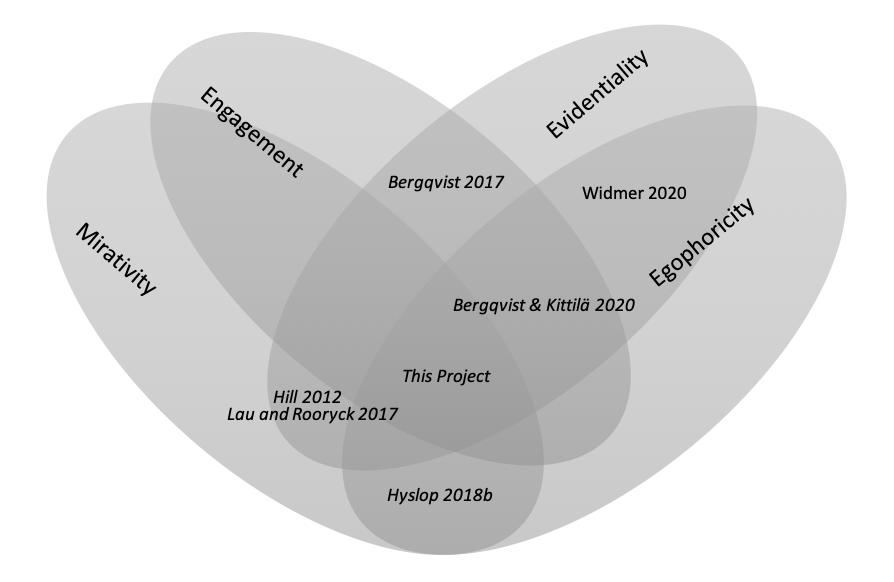
\includegraphics[width=\textwidth]{LitVenn.png}
    \caption{Examples of publications examining the crossovers between phenomena}
    \label{fig:LitVenn}
\end{figure}


\chapter{Background of Trans-Himalayan Languages}\label{c:THOverview}

\section{Introduction}
The \lfam\ family, also referred to as Tibeto-Burman or Sino-Tibetan, is a primary language family spoken throughout parts of Asia, centering on the Himalayas and extending to the south-east through Myanmar and the Shan Hills, to the north through to the northern edge of the Tibetan Plateau, and to the west into the Karakoram mountains and Baltistan. Languages of this family are also spoken throughout China, both historically and as the official language of China, Standard Mandarin (\textit{pǔtōnghuà}). Their overall geographic distribution is shown in \mapref{fig:OverallMap}, showing the family stretching as far north as Northern China (Mandarin, Sinitic), to the western reaches of the Himalayan range in Kashmir in the west (Purik and Balti, Tibetic). In the south, the Karen subfamily stretches south towards the Malay Peninsula, and in the east, more recent migrations have brought Sinitic Languages to Taiwan. The family includes major languages such as Mandarin and Cantonese, both in the Sinitic branch, Burmese, in the Ngwi-Burmese branch, and Tibetan, in the Bodish branch. Additionally, some smaller languages have official status or institutional support such as Dzongkha and Denjongke (Tibetic) in Bhutan and Sikkim respectively. The remainder of the languages in the family are, for the most part, spoken by smaller indigenous communities throughout the region. Glottolog reports almost 500 languages in the family \cite{glottolog}, while \citeA{Owen-SmithHill2013} report around 600, with over 1.4 billion total speakers \cite{ZhangH2020Baye}, approximately 900 million of which are native Mandarin speakers \cite{Ethnologue}. While the majority of the family's speakers exist to the North of the Himalayan range in China, this statistic is a result of the overwhelmingly large number of speakers of Sinitic languages, specifically Mandarin and its dialects. The greatest area of linguistic diversity, on the other hand, falls to the South, in the Eastern Himalaya region covering Eastern Nepal and far North-Eastern India, in particular in the Shan Hills \cite{BlenchPost2014}.

This chapter comprises an overview of the history of research into the \lfam\ family in Section \ref{s:historyofresearch}, both in the Western tradition and otherwise, a major part of which is the growing body of grammatical description that provides a foundation for this project. It also provides an overview of some contemporary ongoing discussions and research in the field in Section \ref{s:THOverview:CurrentResearch}, and establishes the stance taken in this project with regards to these disagreements. Within this, Section \ref{ss:Methods:Bayesian} compares a number of proposed phylogenies, in particular those developed through Bayesian analyses in \citesA{Sagart2019Baye}{ZhangM2019Baye}{ZhangH2020Baye} and discusses some potential issues with the conclusions they draw. It will also consider the usefulness of these methodologies and their results both in the development of a representative sample and in linguistics in general. Lastly, it discusses the work that has been undertaken in the historical domain, looking both at surviving primary sources of historical languages, as well as the current extent of reconstructions of proto-languages.

\begin{map}
\centering
\includegraphics[width=\textwidth]{FullExtent.png}
\caption{The approximate full extent of the \lfam\ languages, missing some parts of the People's Republic of China, and of Taiwan. There are areas inside this extent where \lfam\ languages are not spoken, or where non-Trans-Himalayan languages are spoken (e.g. Kra-Dai, Austroasiatic, Mon-Khmer, Indo-European).}
\label{fig:OverallMap}
\end{map}


\section{History of Research into \lfam\ Languages}\label{s:historyofresearch}
\subsection{Pre-European scholarship}
Linguistic research is no new innovation in the Himalayas and Eastern Asian. Scholars have written about language and its history and use well before the arrival of any Western Academic Tradition to the region. Literary traditions have existed in a number of regions for many centuries, and much of this literature informs contemporary linguistic research.

Old and Middle Chinese Rime Books, books grouping characters by their pronunciations, have been widely used as sources informing contemporary reconstructions of the languages \cite{Baxter1992}. The books were composed as early as the 2nd Century CE, through to the 9th. Due to the (generally) non-phonetic nature of the Chinese writing system, these books were compiled to create some record or method of instruction into the pronunciation of each character, by sorting each character in terms of its onset and rime \cite{Ji2021}.

There is similarly a very longstanding tradition of linguistic research in Tibet. Perhaps the most important of these are the \texttibetan{སུམ་ཅུ་པ} \textit{Sum cu pa} and \texttibetan{རྟགས་ཀྱི་འཇུག་པ} \textit{rTags kyi 'jug pa}, both attributed to 7th century scholar Thönmi Sambhoṭa, who is also credited with the development of the Tibetan writing system \cite{MuellerWitter2009}. These treatises comprise early grammatical descriptions of the language at the time, and are, at least according to legend, the only two survivors of a corpus of eight written by Thönmi Sambhoṭa \cite{Miller1963}, and are accompanied by a tradition of more recent of commentaries and translations \cite{Chashab2008}. There have been questions raised as to whether or not the attribution of these works to Thönmi Sambhoṭa is historically accurate, both for the grammatical treatises and development of the script. Arguments have been made that the treatises could have been written several hundred years later than legend reports \cite{Miller1963}. Aside from various historical inconsistencies or points of uncertainty when dealing with primary sources, \citeA{Miller1963} notes that the \textit{Sum cu pa} and \textit{rTags kyi 'jug pa} alone cover both the syntax and morphology of the language respectively \cite{Chashab2008}, leaving the question of what the other six treatises would have actually addressed. There seems to have been little reference in the Tibetan tradition as to the contents of this lost body of work, suggesting that they may never have existed.

While it is important to note this history of research and grammatical description in China and Tibet, there is little evidence of grammaticalised epistemic marking in Old Tibetan, in that the modern evidential-egophoric paradigm had not yet developed \cite{Hill2014} (though some distinctions have been described for Middle Classical Tibetan \cites{Zeisler2018}{Oisel2024}). Similarly, it does not appear that any relevant grammatical phenomena were present in Old Chinese (which is, at least at this stage, similarly the case for the modern Sinitic languages), with the exception of adverbs marking epistemic modality\footnote{There is a question surrounding the definition of an adverb versus a particle (that is, lexical versus grammatical) that I will not attempt to answer.} \cite{Pulleyblank1995}. As such, this early research provides no extra data for analysis. That said, it does mean, at least in the case of Modern Tibetan, the evidential-egophoric system is an innovation or areal borrowing, rather than a system that might have been inherited from any proto-language, Tibetic or earlier. Further historical languages with surviving records but lacking contemporaneous linguistic research are presented in Section \ref{s:AncientLiteraryLanguages}.

\subsection{European scholarship}
In contrast to this centuries-old body of research into Tibetan and Chinese grammar and phonology, the history of Western research and interest into the family is only some 200 years old. A `Tibeto-Burman' language family containing Chinese, Tibetan, and Burmese, and excluding geographically close language groups such as Kradai, Austroasiatic was first proposed by Julius von Klaproth in 1823 \cite[12]{VanDriem2014}, though this was by no means a widely accepted theory until much later. Much of the other earliest research into the language family by Western Scholars was built on racist ideas of language structure, equating the lack of inflection in group such as the Sinitic and Tai languages were a result of a lack of mental capacity \cite[13]{VanDriem2014}. Comparative evidence of a link between Tibetan and Chinese was not found, however, until the early to mid 20th Century, with the work of Robert Schafer, first published in 1939. This work, however, still included the Tai languages in the Phylum, a clade which would not be readily dropped from the family until much later \cite{Matisoff1991}. \citeA{Handel2008} reports another source around the same period, a 1937 survey of the languages and dialects of China by Li Fang-Kuei, that also included neighbouring families such as Tai and Miao-Yao, which is noted in the editorial of its 1973 republication to have been an influential piece of literature in the area of study through the mid 20th Century \cite{Li1973}.

The past few decades have seen a rapid increase in the amount of research on the \lfam\ family in the Western Academic Tradition, though research has been conducted to some extent since the early 19th Century \cite{VanDriem2014}. In 1991, \citeA{Matisoff1991} suggested that the field was no older than 50 years, and had only seen substantial growth since the late 1960s. This recent growth in research can be seen in \figref{fig:PublicationsChart}, which shows the number of publications on \lfam\ linguistics by year, as indexed by the Glottolog database \cite{glottolog}. The drop-off in the most recent years can in part be attributed to the fact that the data for this graph were collected before a year was complete, and as such more recent publications from the first half of the year might not have been added into the Glottolog database. The rise that can be seen starting in 1950 and accelerating substantially over the past 20 years can be attributed to a number of factors. The past few decades have seen an increase in the accessibility of many of these areas, physically and legally. Many of the states in North Eastern India only opened to international researchers within the past decade, allowing a substantial increase in research output focused on this region \cite{BlenchPost2014}. A similar situation can be seen in Bhutan, where research access has historically, and even to the present, been severely restricted (Hyslop, p.c.). It is no coincidence then that many of the subfamilies with very limited description are in this region (e.g., Gongduk, Lhokpu in Bhutan (see Sections \ref{ss:THOverview:Subfamilies}, \ref{s:Methods:FieldMethods}), Digarish, Mudzuish in North-Eastern India.) This uneven descriptive coverage and its implications for this project are further discussed in Sections \ref{ss:THOverview:HighLevelStructure} and \ref{ss:THOverview:Subfamilies}.


\begin{figure}

\centering
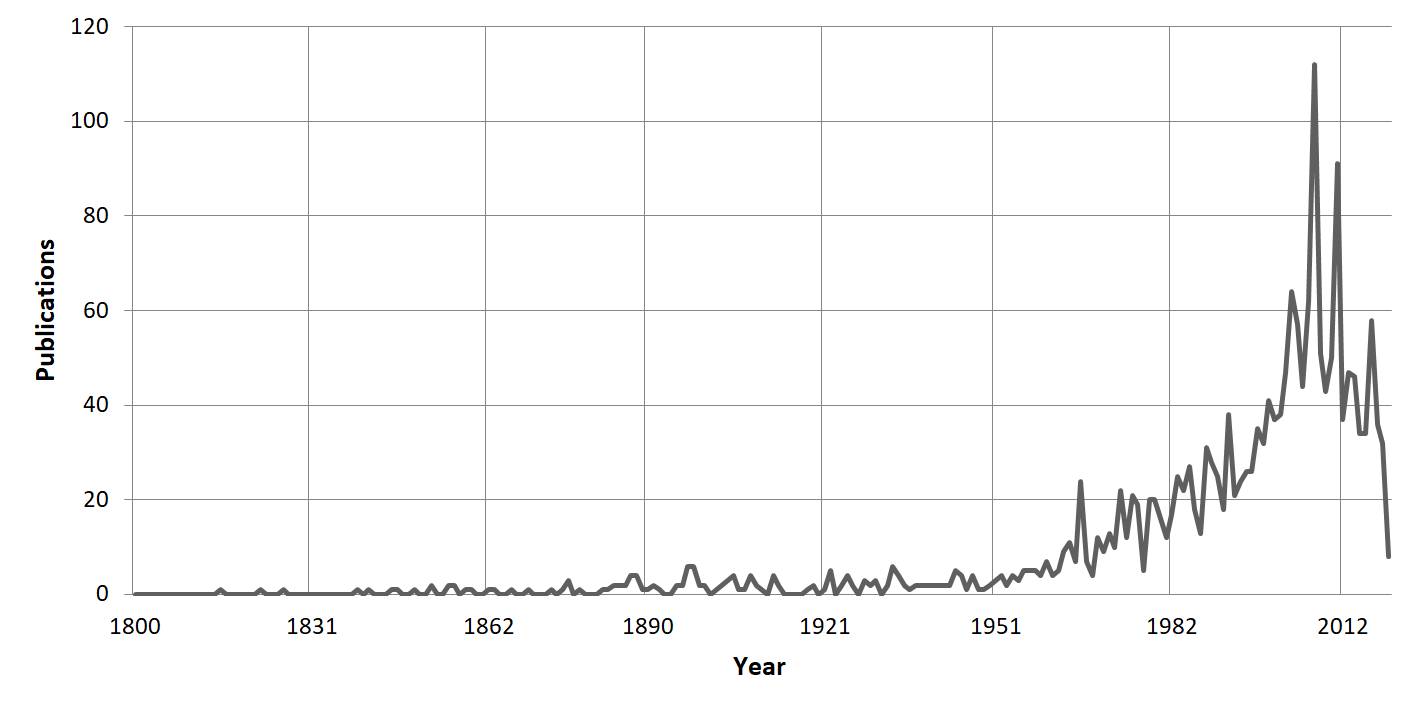
\includegraphics[width=\textwidth]{PublicationsChart.png}
\caption{Number of publications on the \lfam\ family recorded in the Glottolog database by year up to mid 2021 \cite{glottolog}}
\label{fig:PublicationsChart}
\end{figure}


\subsection{Dialects or Languages?}\label{s:DialectsorLanguages}
The question of the distinction between a language and a dialect is, of course, all pervasive to linguistics. Different interpretations of this distinction in different research traditions and political systems in the region have created an imbalance in the definition of languages and dialects in the family. \citeA{LaPolla2016} suggests that languages predominantly researched by linguists in the Chinese academic sphere, especially in the Sinitic branch, tend to more commonly be considered dialects of single broader languages, while languages researched by other linguistics, namely in the Indian academic sphere, tend to be considered separate languages in a more closely related subfamily. Anecdotally, I was once told by a Bhutanese person who heard about my research that they believed Bhutan to have 90 different languages, a figure which would require an incredibly fine-grained approach to the definition of languages as opposed to dialects to be true (\citesA{vanDriem1994}{Hyslop2016} suggest a number closer to 20).

This is also reflected at a policy level, in terms of how governments identify and classify various ethnolinguistic groups. \citeA{Bradley2002} give an extreme example from the Eastern Indo-Chinese border, where India officially identifies over 50 different `scheduled tribes' or ethnic groups, which are all grouped into a single Luoba `nationality' across the border by China.

While these two tendencies don't necessarily produce differing results in terms of isolated descriptions (descriptions of separate `dialects' of languages spoken in China have been conducted similar to descriptions of separate `languages' spoken elsewhere \cites{Lai2017}{TaylorAdams2020}), it can cause skew at a typological level, as there is a possibility that similarly divergent groups of `languages' or `dialects' will be identified as its own subfamily if spoken in India, but not in China. This has been raised as a potential criticism of \citeA{VanDriem2014} \cite{LaPolla2016}, and presents a potential issue in sampling for this project. That is, will a region of high linguistic diversity be missed or underrepresented as it is classified in such as way that seems to (deliberately or otherwise) minimise recognition of this diversity?


\section{Current State of Research}\label{s:THOverview:CurrentResearch}
\subsection{State of description}\label{ss:Description:StateOfDescription}
The level of coverage in the description of languages across the \lfam\ subfamilies varies greatly, ranging from subfamilies with over a hundred published grammars, to a number with no published comprehensive grammars, or even no published description at all. In order to compare the state of description across the family and illustrate the disparities, data on language numbers (also presented in Table \ref{t:Methods:SubfamilyLanguageCount}) as well as on published literature on each language has been collected from Glottolog \cite{glottolog}. Specifically, the number of unique\footnote{This excluded both exact repetitions in the database where two sources have had the same publication under slightly different names (e.g., with or without middle names or initials), and cases where a two grammars of the same language by the same author are listed, usually because of a thesis which has subsequently been turned into a book. This latter case has been excluded as, while there are likely differences between the two publications, they do not represent the greater level of coverage in the literature that would be seen from a second grammar being written out of an entirely separate project.} publications categorised in Glottolog's database as ``Grammar'' has been counted for each subfamily, as well as the languages of these publications. These figures are estimations, given that the boundary between the distinction in the database between ``Grammar'' and ``Grammar Sketch'' is not a clear line,\footnote{Glottolog does define the categories as ``~150 pages and beyond'' and ``~50 pages'' \cite[Glossary]{glottolog}, though this is not always reflected in practice.} and that it is relying on Glottolog's very broad but not necessarily perfect coverage of the literature. Similarly, the figures used for the numbers of languages are, of course, also estimations using Glottolog's categorisation. Finally, the database covers publications on grammars dating back at times to the 19th century, which may not be considered up to contemporary standards in terms of linguistic analysis. As such, these figures can certainly be illustrative in a broad sense, showing the differences in documentation levels in general terms, but cannot be seen as precise figures for any further detailed statistical analysis.

The highest coverage was recorded for Meithei, an internal isolate. Glottolog recorded eight unique grammars for the one language, with the earliest being a description by Arthur John Primrose published in 1888\nocite{Primrose1888}. This is, however, by some measure the highest number, with the next highest ratio of languages to grammars seen for the Sinitic subfamily, which has 4.46 grammars for each language.\footnote{116 grammars across 26 languages.} Figure \ref{f:Description:SubfamilyCoverageGraph} shows the ratio of overall grammars per language in each subfamily. Four subfamilies show a ratio of one, meaning there is an equal number of published grammars on the subfamily and languages in the subfamily on Glottolog. This does not mean, however, that every language in the subfamily has been described, as levels of description can vary widely within a given subfamily. While an internal isolate, the example of Meithei is a good explanation of why this is possible, where multiple grammars have been written on the one language. Similarly, there are cases where the authors of grammars might consider two varieties different languages, or at least sufficiently different for a separate grammar, but the varieties are grouped as one language on Glottolog. For example, of the two English-language grammars on Tshangla, another internal isolate, \citeA{Grollmann2020} is specifically about the Bjokapakha variety, while \citeA{Andvik2010} covers Tshangla more generally, as external influences prevented him from working with any single given speech community or village. In other cases, for instance with \citesA{Gates2021}{Honkasalo2019} writing about Eastern Geshiza and Mazur Stau, it is not necessarily clear whether or not the two rGyalrongic varieties described ought to be considered different languages or not, but are in any case considered grammars of the same language in this analysis and in the source of the data \cite{glottolog}. In this example, \citeA[1]{Honkasalo2019} refers to the specific subgroup within rGyalrongic as the ``Horpa languages'', while \citeA[12]{Gates2021} uses the same, as well as the more agnostic term ``Horpa lects''.

\begin{figure}
        \centering
        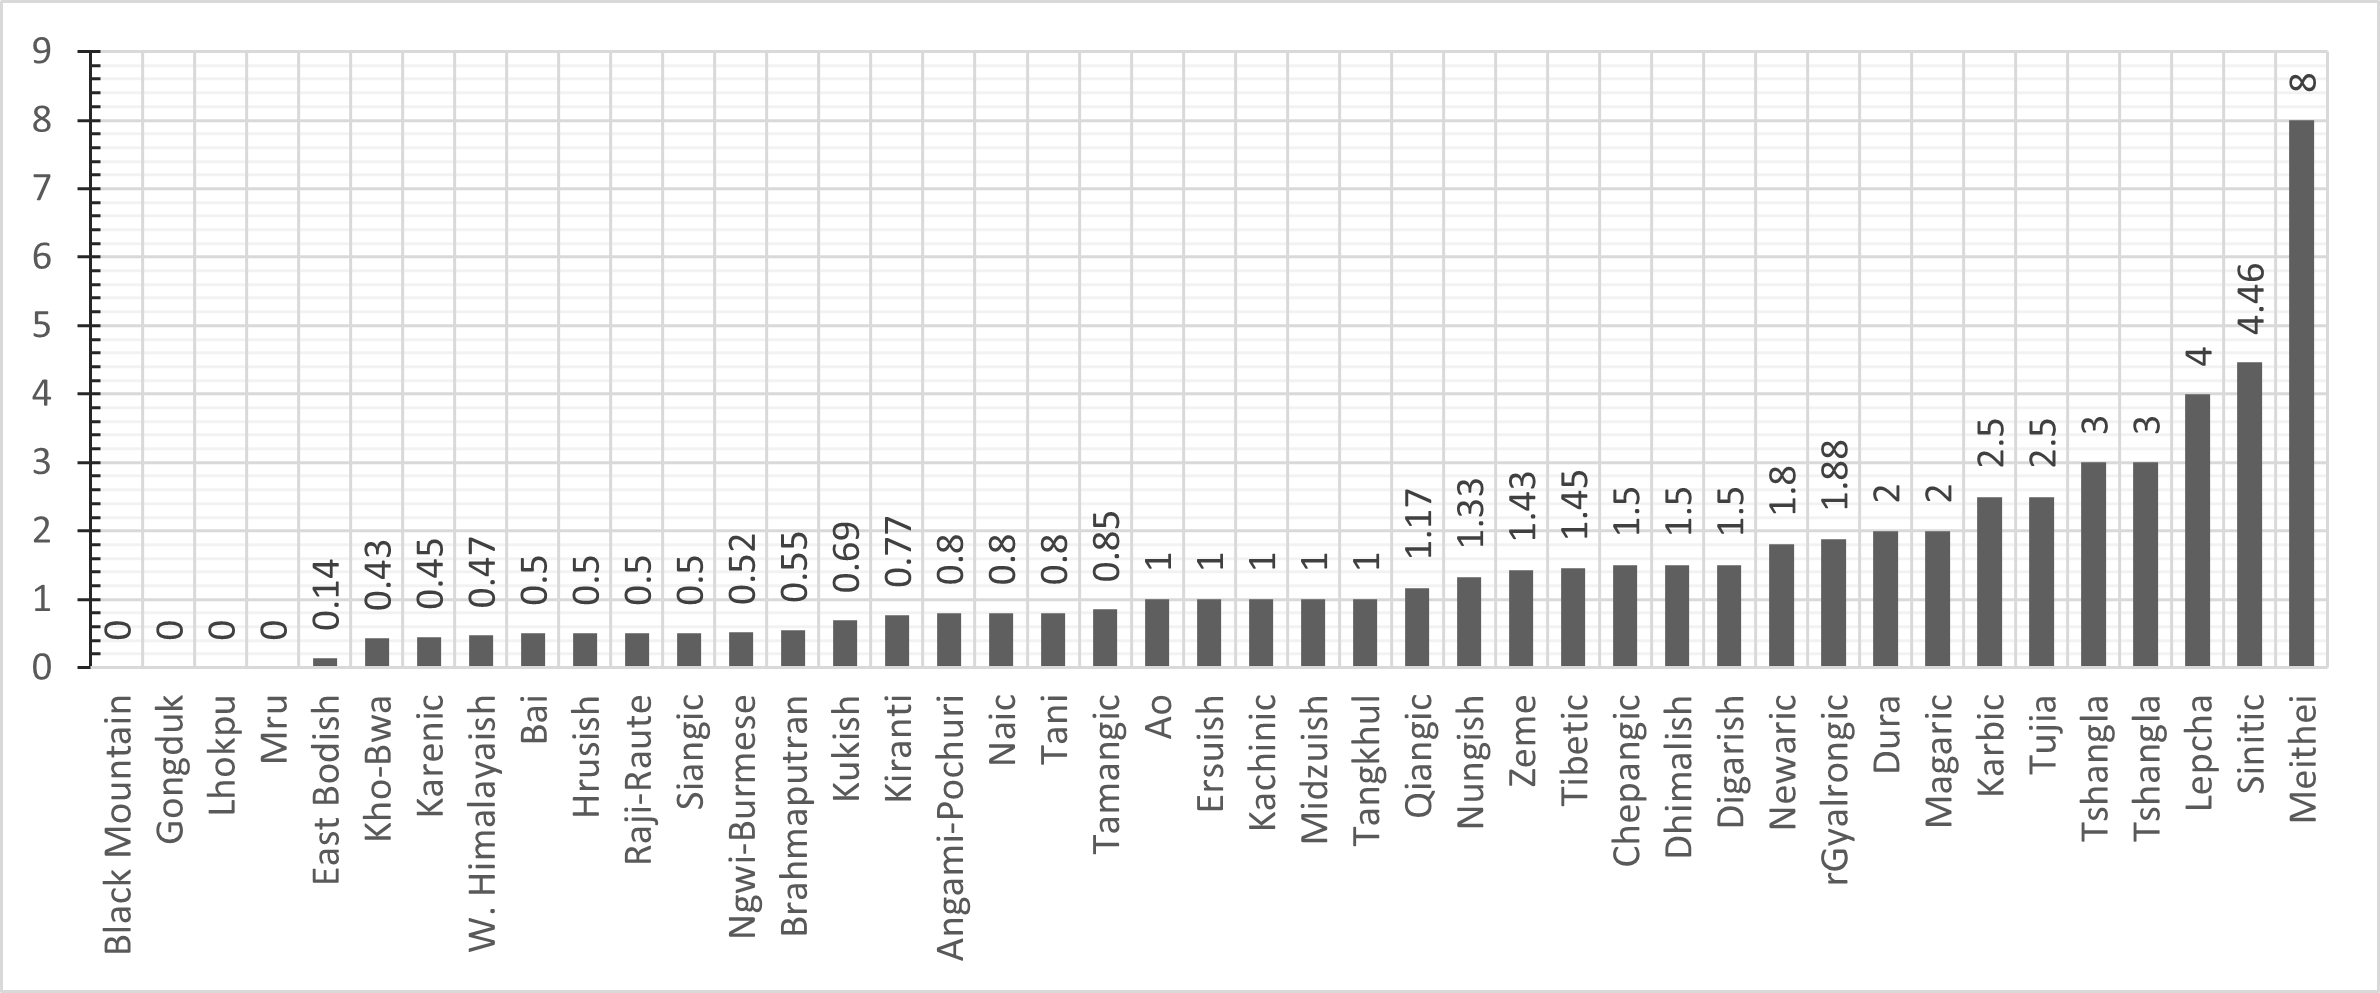
\includegraphics[scale=0.7]{Subfamily Coverage Graph.png}
        \caption{The ratio of overall grammars per language for each of the subfamilies, sorted from lowest to highest.}\label{f:Description:SubfamilyCoverageGraph}
\end{figure}

A comparison of the metalanguages of the literature in this dataset can also reveal some trends, and more specifically can reveal some gaps in the data that is available to this project, given it was limited to literature written in English with some exceptions in texts written in French or German, e.g. \citeA{Lai2017}. This data is presented in Figure \ref{f:Description:SubfamilyCoverageByLanguage}, showing the metalanguages used as a percentage of the total grammars in the dataset. Unsurprisingly, the families with higher levels of literature in Chinese, namely Bai, Digarish, Ersuish, Kho-Bwa, Mizduish, Ngwi-Burmese, Nungish, Qiangic, rGyalrongic, Sinitic, and Tujia, are all at least in part spoken in China. The Digarish, Kho-Bwa, Midzuish, and Nungish branches are all spoken partly outside of China (or in contested areas), specifically in all three cases around the tri-point between China, Myanmar, and the Indian state of Arunachal Pradesh. In these cases as well, the Chinese literature comprises one or two of a total of three or four publications. The higher level of use of French as a metalanguage in the rGyalronic subfamily (4 out of 15) can be attributed directly to the research and teaching of Guillaume Jacques, as three of the items are doctoral theses over which he was supervisor, and the final is his own grammar of Japhug \cite{Jacques2021}.

\begin{figure}
        \centering
        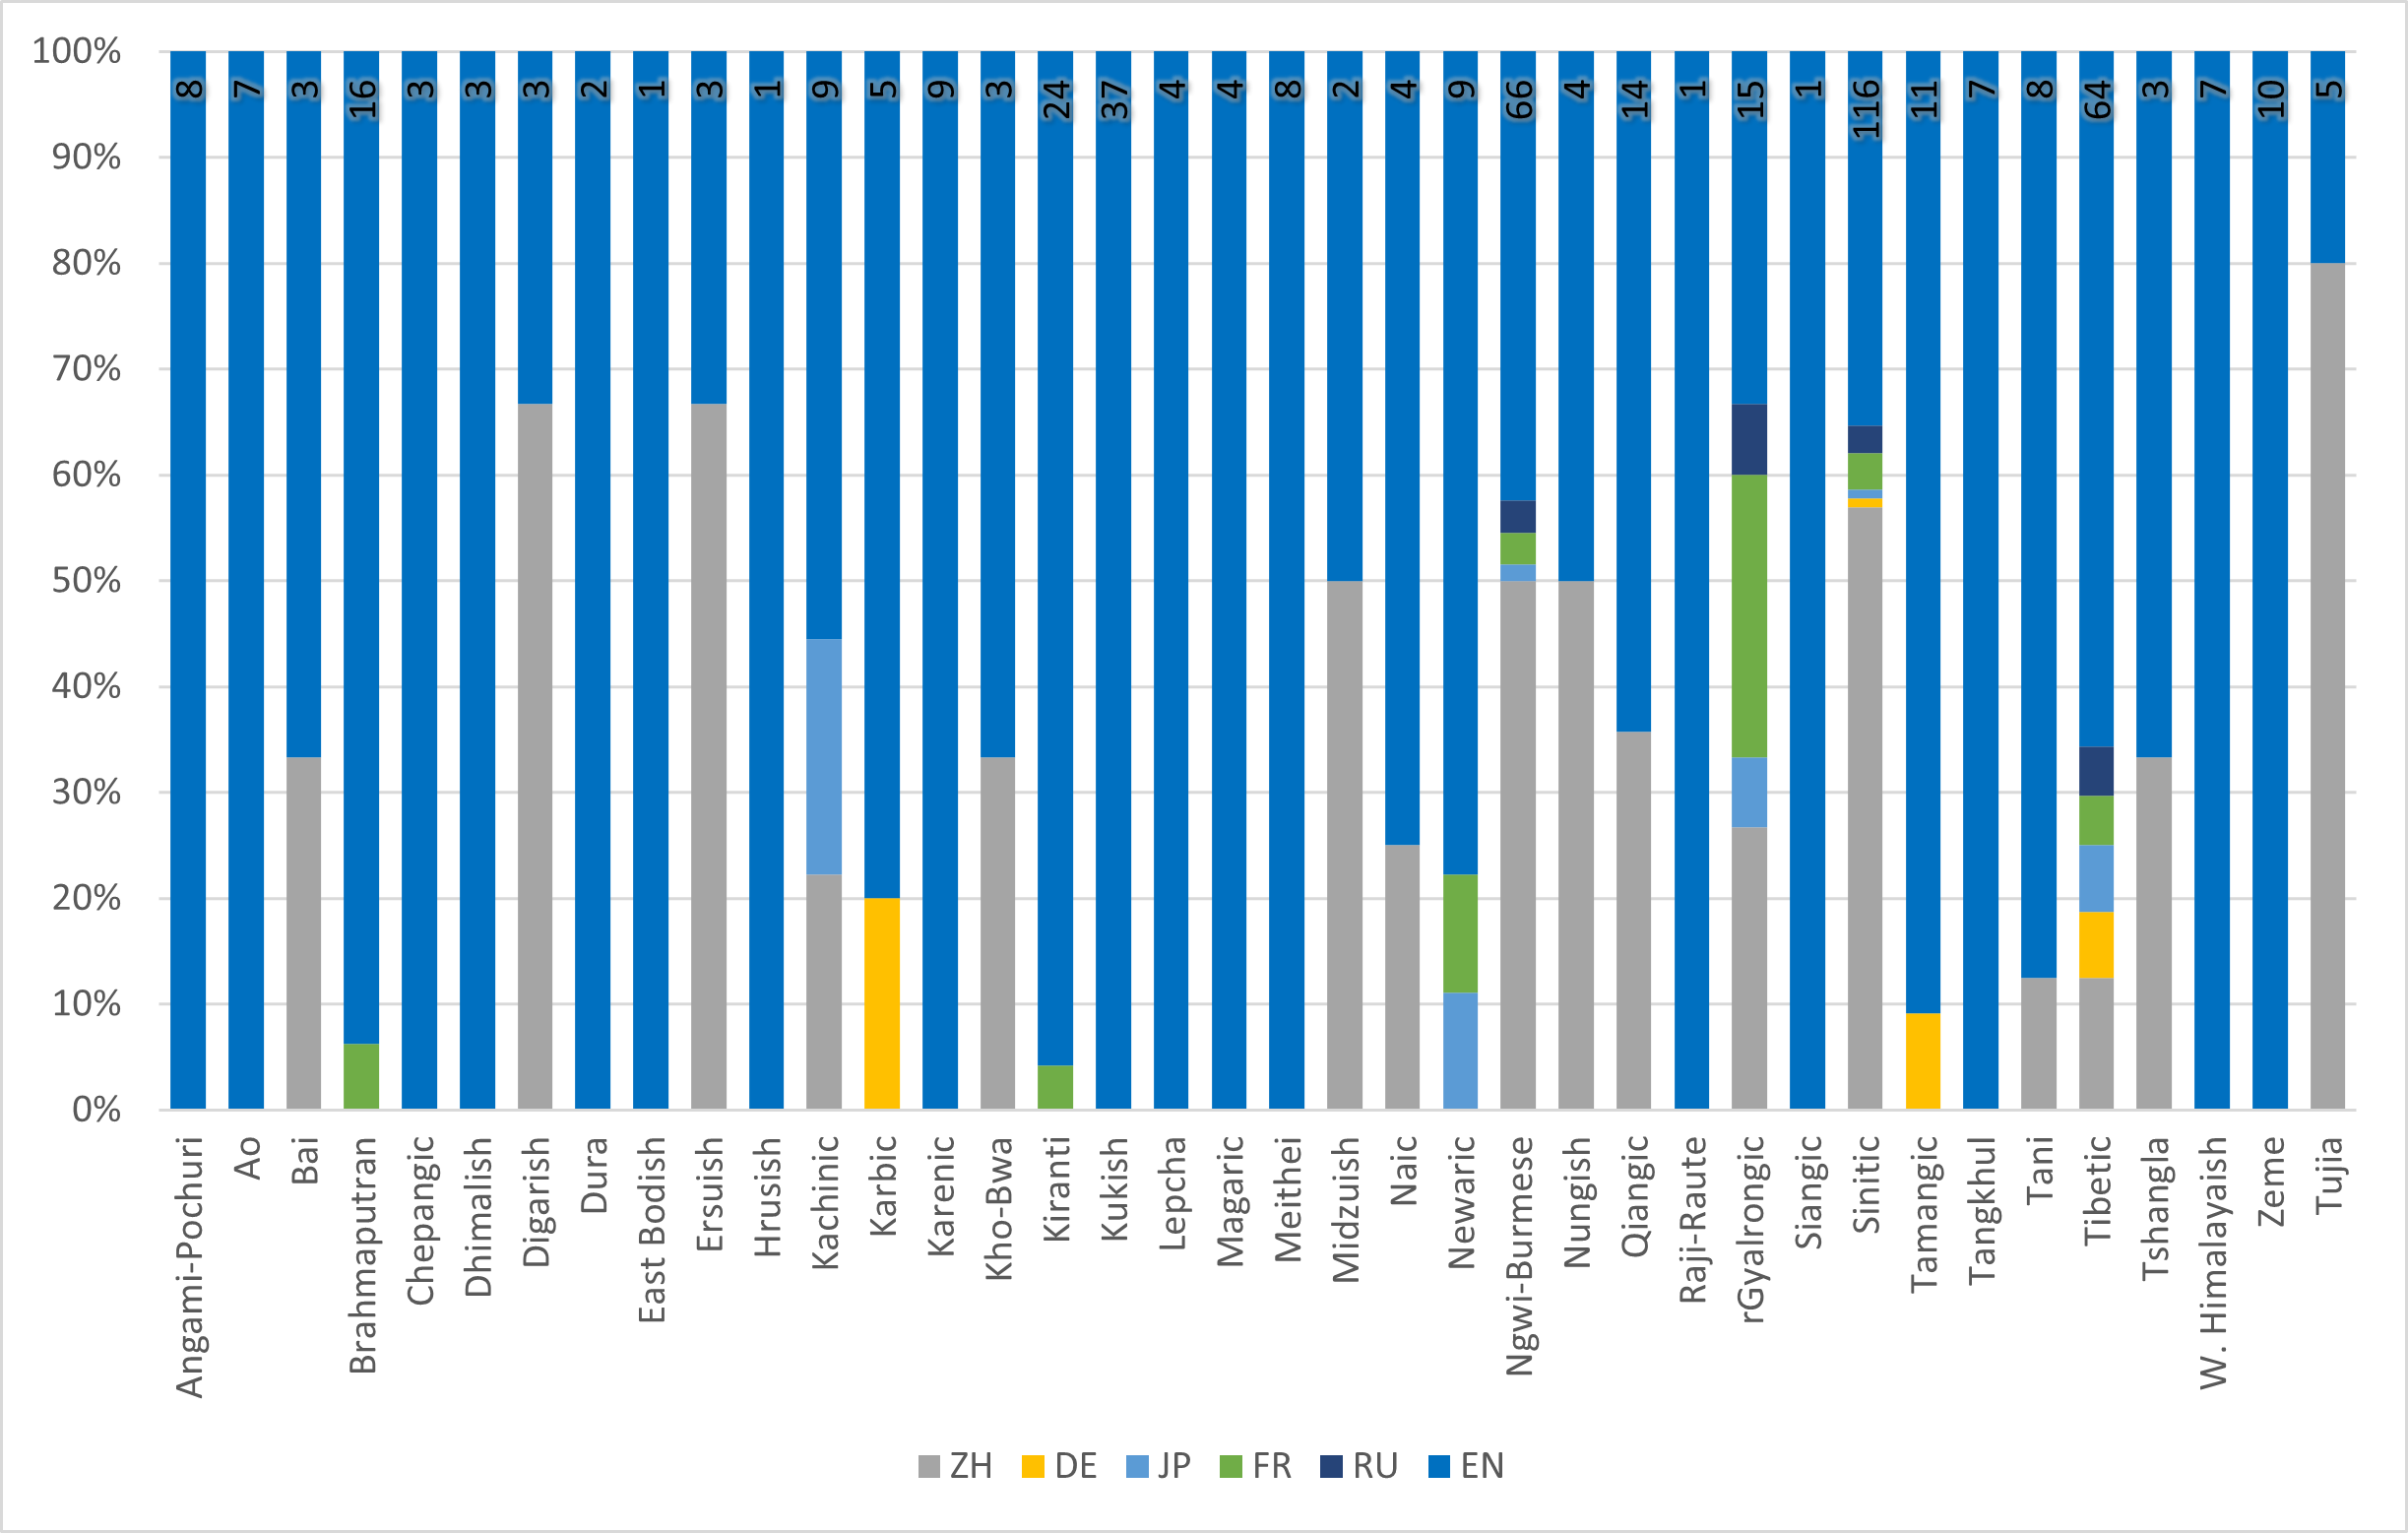
\includegraphics[scale=0.7]{Subfamily Coverage By Language.png}
        \caption{Distribution of metalanguages as a percentage of the total grammars in each subfamily. The number at the top of each subfamily is the total number of grammars in the dataset per sufamily.}\label{f:Description:SubfamilyCoverageByLanguage}
\end{figure}

Thus far, the literature being referenced in this analysis has broadly been referred to as ``published'' or as a survey of ``publications'', however it is worth noting that this also includes both masters and doctoral theses, which have not technically been published or peer reviewed in the same sense as a book would. While this is not to say that a masters or doctoral thesis is inherently less reliable than a published book, masters theses in particular are inherently shorter and less detailed. It was not feasible to annotate all of the grammars in the dataset for their initial origin in these terms, but assuming a higher number of masters and doctoral students undertaking descriptive projects than degree-holding academics undertaking such projects to the point of a published grammar, it can be assumed that theses comprise a substantial if not majority portion of the dataset.\footnote{While this rings true in the current, I suspect that this has not always been the case. Additionally, the rise of theses being readily available online has made them more accessible, and potentially more common in the Glottolog database.} To compare only the data collected for the larger analysis in this project, discussed in Section \ref{s:Methods:Collection}, about 40\% are masters or doctoral theses, and theses were generally only used where no formally published book was available.

\subsection{Situating the Sinitic Branch in the Family}\label{ss:THOverview:HighLevelStructure}

Current opinion on the structure of the family in the literature is strongly divided, into two main schools of thought, predominantly centred on the highest-level division in the family genealogically. One school of thought suggests that the family is divided into two primary branches: `Sinitic' and `Tibeto-Burman'. Alternatively, some scholars argue that this binary division is incorrect, and that the Sinitic subfamily exists at a lower level within the overall family. These two mutually exclusive hypotheses will be henceforth referred to as the Sinitic-Divergent and Other-Divergent hypotheses.

A number of recent studies have found evidence in favour of the Sinitic-Divergent hypothesis through computational methodologies \cites{ZhangM2019Baye}{ZhangH2020Baye}{Sagart2019Baye}, namely Bayesian analyses and methodologies from fields of genetics, using cognate sets as an equivalent to genetic markers. While these three papers are able to agree on their support of the Sinitic-Divergent hypothesis to various extents, they otherwise disagree on the internal structure of the Tibeto-Burman branch and the time-scale of the family as a whole. \citeA{Sagart2019Baye} report an origin around 7,400 years BP, with a millet-farming urheimat, in North-Eastern China. \citeA{ZhangM2019Baye} on the other hand reports a slightly younger mean age (about 5,800BP) and an urheimat much further south-west, in the eastern reaches of the Tibetan Plateau. Finally,  \citeA{ZhangH2020Baye} suggest an even earlier origin, at 8,000 years BP, and while not providing a clear urheimat, they do suggest that the Sinitic/Tibero-Burman division occurred prior to the development of widespread agriculture in China.

A number of potential issues in these methodologies have been identified by various researchers. \citeA{ZhangH2020Baye} themselves highlight some methodological concerns in \citesA{ZhangM2019Baye}{Sagart2019Baye}, namely surrounding the representativeness of their datasets. They suggest that their dataset presents a more evenly distributed cross-section of the language family by subfamily, with a lower standard deviation in percentage of languages in each subfamily sampled \cite{ZhangH2020Baye}. They also note that \citeA{Sagart2019Baye} contains no data at all from the Karenic or Naga subfamilies, with Karenic languages being spoken geographically much further south than other languages in the family.

This criticism, however, can extend to any study aiming to computationally analyse high level structures of any language family. That is, if a dataset is missing particularly linguistically or geographically divergent data, it is difficult to see it as an accurate representation of the data. Similarly, if data from only one language from a given sub-family is included, but many languages from another, that dataset might be similarly skewed. \citeA{ZhangH2020Baye} notes this as an issue in \citesA{ZhangM2019Baye}{Sagart2019Baye}, and reports an a more even coverage of each subfamily than in the two previous studies. However, this relies on the subfamilies as given in the paper being representative of the actual subfamilies that exist from a historical perspective. There is a degree of a circular logic here. In order to create an even sample of the language family by subfamily, one needs first to know what these subfamilies actually are, which is in many ways exactly what these studies are trying to discover.

\citeA{ZhangH2020Baye} also only report subfamily coverage for a small set of subfamilies, grouping a large number of other languages into the category ``isolates'' and as such ignoring any subfamily relations they may have. In some cases, such as with Tujia or Meithei, this agrees with other literature such as \citeA{VanDriem2014}, though in other cases it seems to fail to consider the language's other close relations. For instance, Kinnauri is listed as an isolate in the list of languages, despite being classified in a separate West Himalayish subfamily by both \citesA{VanDriem2014}{Thurgood2017STIntro}, a subfamily with, in addition to Kinnauri, at least 14 other languages \cite{glottolog}. A similar issue exists with the Kachinic languages, which are represented solely by the so-called `isolate' Jingpo (at the exclusion of 8 other languages), as well as with the rGyalrongic languages, which are represented by Jiarung, Daofu Horpa, and Ergong, all of which are given as isolates despite being grouped together in wider literature \cites{Honkasalo2019}{Gates2021}.\footnote{A pervasive challenge in research on the \lfam\ family is the lack of agreement on language names. `Jiarung' most likely refers to the rGyalrongic languages here, though the core group of the subfamily is varyingly referred to as a group of languages or dialects of a single language. See Section \ref{s:DialectsorLanguages} for further discussion.}

\subsection{Name of the Family}

This uncertainty surrounding the high level internal structure of the language family also has implications for the name of family itself, in that the historically most widespread name `Sino-Tibetan' specifically references the Sinitic-Divergent hypothesis. A number of alternatives to this have been suggested, either to actively reject the Sinitic-Divergent hypothesis or to remain agnostic. `Tibeto-Burman' has been used fairly widely as an alternative name for the family as a whole, in contrast to Tibeto-Burman as the non-Sinitic branch of a Sinitic-Divergent Sino-Tibetan family \cite{vanDriem2007a}. While this no longer supports a Sinitic-Divergent structure for the family, it also seems to suggest some level of primacy or greater importance to Tibetan and Burmese languages, one of the very issues initially identified with the term Sino-Tibetan. A second alternative, `Trans-Himalayan', has been more recently suggested, avoiding reference to any specific language to avoid any such suggestions of internal structure or greater importance in certain languages or subfamilies \cite{BlenchPost2014}. Here, `Trans-Himalayan' refers to the geographic distribution of languages in the family across entire Himalayan range, and well to the North and South. A potential point of confusion with this name is the inconsistency in meaning between this term and the use of `trans' in wider toponomy. For example, `Transalpine' traditionally refers not to the area across \textit{both} sides of the Alps, but on the \textit{other} side (from Rome), and is contrasted with `Cisalpine' (on \textit{this} side of the Alps).

The term \lfam\ is used in this thesis \lfamreason\

\subsection{Overview of Subfamilies}\label{ss:THOverview:Subfamilies}

George van Driem (2014) \nocite{VanDriem2014} presents a large set of subfamilies that are widely agreed on to exist, while avoiding any claims about other internal structures. These subfamilies are illustrated in \figref{fig:SubFamMap}. Subfamily names have been taken directly from \citeA{VanDriem2014}, with the exception of Lolo-Burmese, for which the term Ngwi-Burmese will be used in line with publications such as \citeA{Donlay2019} and \citeA{GonzalezPerez2022}, following \citeA{Bradley2005}.

While \citeA{VanDriem2014} is able to represent well established subfamilies, uncertainties in the literature arise still in areas with limited description. While there is often a general consensus of which languages are a member of the family and which are isolates or members of other families such as Tai, Austroasiatic, or Indo-European, \citeA{BlenchPost2014} suggest that the lack of research in some areas mean that languages assumed to be \lfam\ simply cannot actually be proven as such (e.g., Hruso, Hrusish: India). They similarly report that some languages in the region are so divergent, it is unclear if they are \lfam\ or languages from a pre-existing family that have undergone heavy \lfam\ influence (e.g., the Siangic subfamily \cite{Post2011}).

\begin{map}

\centering
\includegraphics[width=\textwidth]{SubFamilies.png}
\caption{Approximate geographic distribution of van Driem's (2014) subfamilies. Subfamilies with only one language, or two languages that are not geographically contiguous are represented as single points.}
\label{fig:SubFamMap}
\end{map}

The subfamilies proposed by \citeA{VanDriem2014} can be split into two groups, true subfamilies and internal isolates, that is, groupings with containing multiple languages as opposed to those containing only one. The ten \lfam\ isolates are the following.


\begin{itemize}
    \item Black Mountain Mönpa, aka `Olekha, is a moribund language spoken in Central Bhutan \cites{vanDriem1995}{Hyslop2016}
    \item Dura is a likely extinct language historically spoken by the Dura people in Lamjung district, Nepal \cite{Schorer2016}
    \item Gongduk is a largely undescribed language spoken in South-Eastern Bhutan spoken by approximately 1000 people in Gongdü Gewog \cite{Bodt2012}.
    \item Lepcha is spoken by 30,000-50,000 speakers in the Indian state of Sikkim and the surrounding regions in Bhutan, Nepal, and the Indian state of West Bengal \cite{Plaisier2007}.
    \item Lhokpu is a largely undescribed language spoken by the Lhop or Doya people in South-Western Bhutan, potentially more closely related to the Dhimalish subfamily \cites{Bodt2012}{Grollmann2018}, discussed in greater detail in Section \ref{s:Methods:FieldMethods}.
    \item Meithei, aka Manipuri, is the primary language of the North-East Indian state of Manipur, where it is spoken by well over 1 million people \cite{Chelliah1997}.
    \item Pyu is a historical language, spoken in modern-day Myanmar prior to the spread of Burmese speakers in the 11th Century \cite{Miyake2019}.
    \item Mru is an underdescribed language spoken in the Chittagong Hill Tracts in Bangladesh \cite{VanDriem2014}. It has also been suggested that Mru is closely related to the Anu-Hkongso language spoken on the Bangladesh/Myanmar border \cite{Peterson2017}.
    \item Tshangla, aka Sharchops, is spoken by approximately 150,000 people in eastern Bhutan, where it is used as a lingua franca throughout the region. It is also spoken by populations in Arunachal Pradesh, India and in Tibet, where it is called Dirang Monpa and Mòtuō Monpa respectively \cites{Andvik2010}{Grollmann2018}.
    \item Tujia is spoken by approximately 60,000 of the over 8 million members of the Tujia ethnic group in North-western Hunan Province, PRC \cite{Brassett2006}. In Map \ref{fig:SubFamMap} it is divided into Northern and Southern Tujia, the latter of which is estimated to have fewer than 2,000 speakers.
\end{itemize}

The remaining 32 subgroups contain more languages, ranging from two (e.g., Raji-Raute, Siangic, Midzuish) to upwards of 100 (Ngwi-Burmese), and can be seen in \figref{fig:SubFamMap}.

The coverage of literature on the other subfamilies varies substantially from subfamily to subfamily. The Bodic subfamily, for instance, as was discussed in Section \ref{s:historyofresearch}, has a long history of grammatical research, as well as a larger population, leading to generally speaking greater access for researchers. As such there is a very substantial body of work on Bodish languages, ranging from full grammars (such as \citesA{Zemp2018}{Graves2007}{Denwood1999}), to extensive discussions about the meanings of single words (see \citesA{Aikhenvald2012Mirative}{DeLancey2012}{Hill2012}{HengeveldOlbertz2012} for one very prominent example).

The Qiangic languages are another subfamily with a comparatively sizable coverage in terms of literature, and most importantly to this project, data availability, with a number of grammars available \cites{LaPolla2003}{Ding2014}, and further research underway.\footnote{Agnes Conrad is working on a descriptive project of Eastern Minyag, a language traditionally classified as Qiangic (p.c.)} In total, descriptions are available for at least half of the languages in the subfamily according to Glottolog \cite{glottolog}. While many of subfamilies seem to have similar levels of coverage, with Glottolog listing between a third to a half as many full grammars as there languages in the subfamily, a number of the smaller non-isolate subfamilies have received little to no attention from descriptive linguists at all. In other subfamilies, specifically those primarily spoken in China or its border regions, descriptions are often more plentiful but only in Chinese. These include the Ngwi, Midzuish, and of course Sinitic subfamilies, among others, for which only the English (or French in some cases \cite{Lai2017}) literature can be considered in this project. A more in-depth literature review of the state of description in the family can be found in Section \ref{ss:Description:StateOfDescription}.

\subsection{Comparison of Proposed Phylogenies}\label{ss:Methods:Bayesian}

A substantial contribution to the study of \lfam\ languages, and in particular the historical development of the family in genealogical terms, has been a set of studies using computer statistical modelling, namely Bayesian statistics, borrowed from biology to infer the most likely phylogeny for the family. These studies, \citesA{Sagart2019Baye}{ZhangM2019Baye}{ZhangH2020Baye}, draw varied conclusions about the internal structure of the family and the timeline of its development, though all draw the conclusion that the Sinitic subfamily is most likely either the sole outgroup (or, per \citeA{ZhangH2020Baye}, one of two).

Given their disagreement, and the discussion thus far about their methodology, this section will compare the phylogenies provided in \citesA{Sagart2019Baye}{ZhangM2019Baye}{ZhangH2020Baye} to each other, as well as to the Fallen Leaves model \cite{VanDriem2014}. Some other proposed phylogenies, such as that put forward in \citeA{STEDT}, are not included here as they remain largely agnostic about the family's structure outside of a few primary divisions. In Figures \ref{f:Methods:Sagart}-\ref{f:Methods:Zhang2020}, the trees given in their respective sources are reproduced to the subfamily level. That is, the branches are reproduced exactly, but rather than terminating in individual languages (as in \citesA{Sagart2019Baye}{ZhangM2019Baye}{ZhangH2020Baye}), or in other subfamilies, the branches terminate in the equivalent subfamily from the set used in this project given in Table \ref{t:Methods:SubfamilyLanguageCount}. While the branching structure of the subfamilies is accurately reproduced here, the time depth of the various divergences given in the Bayesian analyses is not.

Not every subfamily is represented in every tree, a point which forms part of the criticism of the Bayesian analyses. This occurs for these analyses when a given sample did not include any data from a given subfamily, and therefore does not represent or account for it in the final result. Missing subfamilies for each of \citesA{Sagart2019Baye}{ZhangM2019Baye}{ZhangH2020Baye} are given in Table \ref{t:Methods:BayesMissingSubfamilies}.

\begin{figure}
\centering
  \scalebox{0.35}{\begin{forest} 
   phylogeny,
[\lfam 
[
  [,tikz={\node [draw,red,fit to=tree] {};}
    [Kachinic]
    [Brahmaputran]
  ]
  [Sinitic,tikz={\node [draw,red,fit to=tree] {};}]
]
[
  [
    [Karbi]
    [,tikz={\node [draw,red,fit to=tree] {};}
      [Tangkhul]
      [Kukish]
    ]
  ]
  [
    [
      [Chepang]
      [
        [Tshangla]
        [,tikz={\node [draw,red,fit to=tree] {};}
          [Tani]
          [Digarish]
        ]
      ]
      [Kiranti,tikz={\node [draw,red,fit to=tree] {};}]
    ]
    [
      [W. Himalayish,tikz={\node [draw,red,fit to=tree] {};}]
      [
        [Nungish]
        [,tikz={\node [draw,red,fit to=tree] {};}
          [Tibetic]
          [
            [
              [Qiangic]
              [rGyalrongic]
            ]
            [Ngwi-Burmese]
          ]
        ]
      ]
    ]
  ]
]
]
\end{forest}}
\caption{The \lfam\ family as per \citeA{Sagart2019Baye}, showing the positions of the subfamilies used in this project. Branches with over 80\% posterior probability (that is, branches with high confidence, see ) have been marked with a red box. Time depth has not been reproduced in this tree.}
\label{f:Methods:Sagart}
\end{figure}

\begin{figure}
  \centering
  
    \scalebox{0.3}{\begin{forest} 
    phylogeny,
  [\lfam 
      [Sinitic,tikz={\node [draw,red,fit to=tree] {};}]
      [
          [
            [Karen]
            [,tikz={\node [draw,red,fit to=tree] {};}
              [Kukish]
              [
                [Ao]
                [
                  [
                    [Tangkhul]
                    [Zeme]
                  ]
                  [Angami-Pochuri]
                ]
              ]
            ]
          ]
          [
            [,tikz={\node [draw,red,fit to=tree] {};}
              [Kachinic]
              [Brahmaputran]
            ]
            [
              [
                [Digarish]
                [Tani]
              ]
              [
                [
                  [
                    [Kiranti]
                    [,tikz={\node [draw,red,fit to=tree] {};}
                      [Chepang]
                      [Magar]
                    ]
                  ]
                  [Nungish,tikz={\node [draw,red,fit to=tree] {};}]
                ]
                [
                  [West Himalayish]
                  [
                    [,tikz={\node [draw,red,fit to=tree] {};}
                      [Tamangic]
                      [
                        [Tibetic]
                        [East Bodish]
                      ]
                    ]
                    [,tikz={\node [draw,red,fit to=tree] {};}
                      [
                        [Nàic]
                        [
                          [Ersuish]
                          [
                            [Qiangic*]
                            [rGyalrongic*]
                          ]
                        ]
                      ]
                      [Ngwi-Burmese]
                    ]
                  ]
                ]
              ]
            ]
          ]
      ]
  ]
  \end{forest}}
  \caption{The \lfam\ family as per \citeA{ZhangM2019Baye}. *The phylogeny here does not in fact support these two subfamilies, but rather gives two rGyalrongic languages -- rGyalrong Maerkang (glottolog: Situ) and Caodeng (glottolog: Tshobdun) -- as an outgroup to the Qiangic clade, and two others -- Daofu and Ergong Danba (glottolog: both under Stau-dGebshes) are given as members of one of two Qiangic branches. Branches with over 80\% posterior probability have been marked with a red box. Time depth has not been reproduced in this tree.}\label{f:Methods:Zhang2019}
  \end{figure}

  \begin{sidewaysfigure}
    \centering
    
      \scalebox{0.35}{\begin{forest} 
phylogeny,
    [\lfam 
      [
        [Sinitic,tikz={\node [draw,red,fit to=tree] {};}]
        [
          [,tikz={\node [draw,red,fit to=tree] {};}
            [Lepcha]
            [Kiranti]
          ]
          [
            [
              [W. Himalayish]
              [
                [Digarish,tikz={\node [draw,red,fit to=tree] {};}]
                [,tikz={\node [draw,red,fit to=tree] {};}
                  [Siangic]
                  [Tani]
                ]
              ]
            ]
            [
              [,tikz={\node [draw,red,fit to=tree] {};}
                [Kachinic]
                [Brahmaputran]
              ]
              [
                [Kho-Bwa,tikz={\node [draw,red,fit to=tree] {};}]
                [Hrusish,tikz={\node [draw,red,fit to=tree] {};}]
              ]
            ]
            [
              [
                [
                  [
                    [Magaric*]
                    [Karen,tikz={\node [draw,red,fit to=tree] {};}]
                  ]
                  [
                    [Dhimalish]
                    [
                      [Magaric*]
                      [Chepangic]
                    ]
                  ]
                ]
                [
                  [Karbi]
                  [
                    [Kukish,tikz={\node [draw,red,fit to=tree] {};}]
                    [
                      [Meithei]
                      [,tikz={\node [draw,red,fit to=tree] {};}
                        [
                          [Angami-Pochuri**]
                          [Ao]
                        ]
                        [
                          [Tangkhul]
                          [
                            [Zeme]
                            [Angami-Pochuri**]
                          ]
                        ]
                      ]
                    ]
                  ]
                ]
              ]
              [
                [
                  [Midzuish]
                  [Nungish,tikz={\node [draw,red,fit to=tree] {};}]
                ]
                [
                  [
                    [Tamangic,tikz={\node [draw,red,fit to=tree] {};}]
                    [
                      [Tshangla]
                      [,tikz={\node [draw,red,fit to=tree] {};}
                        [East Bodish]
                        [Tibetic]
                      ]
                    ]
                  ]
                  [
                    [Tujia]
                    [
                      [
                        [rGyalrongic***]
                        [,tikz={\node [draw,red,fit to=tree] {};}
                          [
                            [Ngwi-Burmese†]
                            [Ersuish]
                          ]
                          [
                            [Qiangic]
                            [rGyalrongic***]
                          ]
                        ]
                      ]
                      [Ngwi-Burmese,tikz={\node [draw,red,fit to=tree] {};}]
                    ]
                  ]
                ]
              ]
            ]
          ]
        ]
      ]
    ]
    \end{forest}}
    \caption{The \lfam\ family as per \citeA{ZhangH2020Baye}. In this analysis, a number of van Driem's (2014) subfamilies are divided, with either single or multiple languages separated from the rest of their subfamily. These have been marked (*, **, ***, †) and are discussed in the text. Branches with over 80\% posterior probability have been marked with a red box. Time depth has not been reproduced in this tree.}\label{f:Methods:Zhang2020}
    \end{sidewaysfigure}

As discussed above, for each of the terminal nodes given in Figures \ref{f:Methods:Sagart}-\ref{f:Methods:Zhang2020} (that is, van Driem's fallen leaves), 1-3 languages has been sampled. While initially the intention of presenting Figures \ref{f:Methods:Sagart}-\ref{f:Methods:Zhang2020} was to compare the representativeness of this project's sample against their proposals for a phylogeny of the \lfam\ family, it is clear from \tabref{t:Methods:BayesMissingSubfamilies} that, in all cases, the coverage of this project is substantially larger, especially in terms of smaller language families or internal isolates. Because \citeA{VanDriem2014} categorised the entire family into generally very fine-grained subfamilies, there are no languages in any of the three studies that cannot be categorised into one of the subfamilies used in this project, and therefore that can initially be seen as gaps in this project's sample. Rather, to identify possible gaps in this survery's sample, it is necessary to identify locations where \citesA{Sagart2019Baye}{ZhangM2019Baye}{ZhangH2020Baye} disagree with \citeA{VanDriem2014}. A number of small disagreements are noted for \citesA{ZhangM2019Baye}{ZhangH2020Baye}

We can also consider areas where van Driem's (2014) larger subgroups are presented as multiple smaller subfamilies in the other data. Namely, \citeA{ZhangM2019Baye} divides the Ngwi-Burmese family into three classifications, diverging approximately 2,000 years ago. Taking these three branches (Loloish, Nusu, Burmish) as separate subfamilies for the sake of representativeness, then the sample for this project contains two Loloish (here: Ngwi) languages, one Burmish language, and no Nusu languages. As is discussed above, the Ngwi-Burmese subfamily is the largest by some margin, which gives some credence to a division into multiple smaller subfamilies. However, when considering the estimated age of the subfamily per the Bayesian analyses, the combined Ngwi-Burmese branch is a similar age to many of the other of van Driem's (2014) subfamilies represented in \citeA{ZhangM2019Baye} (which range from ~750 years old for Tani to ~3,000 years old for Kiranti), as well as in \citeA{ZhangH2020Baye}, in which the subfamilies vary in age from ~500 years old (Ersuish) to ~4,500 years old (West Himalayish). This is to say that although there are a great number of contemporary Ngwi-Burmese languages attested, the branch itself does not appear to be any older than many of the smaller branches used in this survey, and as such there is less of a reason to treat it as too large or too high-level.



\begin{table}
  \centering
  \begin{tabular}{l | l | l}
    \hline
    \citeA{Sagart2019Baye} & \citeA{ZhangM2019Baye} & \citeA{ZhangH2020Baye} \\
    \hline
    Angami-Pochuri & Bai & Bai* \\
Ao & Black Mountain & Black Mountain \\
Bai & Dimalish & Dura \\
Black Mountain & Dura & Gongduk \\
Dimalish & Gongduk & Lhokpu \\
Dura & Hrusish & Mru \\
East Bodish & Karbi & Naic \\
Ersuish & Kho-Bwa & Newaric \\
Gongduk & Lepcha & Pyu \\
Hrusish & Lhokpu & Raji-Raute \\
Karenic & Meithei &  \\
Kho-Bwa & Midzuish &  \\
Kukish & Mru &  \\
Lepcha & Newaric &  \\
Lhokpu & Pyu &  \\
Magaric & Raji-Raute &  \\
Meithei & Siangic &  \\
Midzuish & Tshangla &  \\
Mru & Tujia &  \\
Naic &  &  \\
Newaric &  &  \\
Pyu &  &  \\
Raji-Raute &  &  \\
Siangic &  &  \\
Tamangic &  &  \\
Tujia &  &  \\
Zeme &  &
  \end{tabular}
  \caption{Subfamilies not represented in the initial data or results of \citesA{Sagart2019Baye}{ZhangM2019Baye}{ZhangH2020Baye}. Internal isolates are given in italics. * Bai was specifically excluded in this study as the extensive borrowing from Sinitic languages would cause problems for the analysis.}\label{t:Methods:BayesMissingSubfamilies}
\end{table}

The unrepresented subfamilies shown in Table \ref{t:Methods:BayesMissingSubfamilies} are, to an extent, a good indicator for how representative the given samples are. Of course, some of the missing data is unavoidable, and is repeated in this project, namely for Raji-Raute, Gongduk, Black Mountain, and Pyu. \citeA{ZhangH2020Baye} specifically report that Bai (marked with an asterisk in Table \ref{t:Methods:BayesMissingSubfamilies}) was excluded due to high levels of borrowing from Sinitic languages, which causes problems when comparing cognates. For \citeA{ZhangH2020Baye}, this leaves only a few smaller subfamilies unrepresented, and for \citeA{ZhangM2019Baye} a few more, though most are still fairly small or underdocumented. \citeA{Sagart2019Baye}, however, in addition to the smaller or inaccessible subfamilies excluded by the others, has a few more glaring omissions. Namely, no data from any Karenic, Kukish languages were included, nor from the smaller and, at least according to \citesA{ZhangM2019Baye}{ZhangH2020Baye}, closely related Angami-Pochuri and Ao subfamilies. These omissions are, as has been already pointed out in \citeA{Hyslop2020Millet} and even in \citeA{ZhangH2020Baye}, problematic in a quantitative analysis in which a representative sample is a necessity, especially given the much wider coverage of \citeA{ZhangH2020Baye} compared to the two earlier studies. Even in cases where data are simply not available, the large gaps in documentary research across the \lfam\ family may mean that, at this stage, the sort of quantitative statistical research undertaken in these projects is simply not yet viable, at least until a truly representative sample can be developed. Such a sample would ot necessarily have to include data from all of the currently underdescribed languages, but would at least be able to be informed by a better understanding of relationships between families. For instance, if further evidence proves further that Lhokpu can be grouped into a Dimalish subfamily with Dhimal and Toto, then it need not be included separately if that family is already sufficiently represented. Similarly, further research on the other underdescribed languages of Bhutan, Gongduk and Black Mountain Monpa, may well allow them to quite clearly be aligned with existing subgroups, but may also distance them further from any clear classification, further necessitating their inclusion in a representative sample of the family.

There is the potential here, however, for a certain circular logic in developing a sample to be used for research into phylogenies, in that the development of a representative sample needs to be informed by a general understanding of the phylogeny of the family in order to sufficiently and more or less equally survey all areas of the family. This understanding, however, is exactly the outcome the research itself is trying to reach. This is further confounded by the uncertainty the studies discussed here have around any reconstructions to deeper time depths, as is discussed below.

Only briefly discussed in \citeA{ZhangH2020Baye} is the statistical confidence surrounding the various bifurcations given in the study's proposed phylogeny. While the study does not suggest that the given tree is clearly correct, it does suggest that the results of the analysis could be used to inform further studies into the history of the people of the Himalayas \cite[5]{ZhangH2020Baye}. The posterior probability of a given divergence is the calculated likelihood of the given branch being valid given the input data and starting parameters ranging from 0 (no  confidence) to 1 (complete confidence) \cite{Alfaro2006}. It can be seen as the probability that everything under a given branch belongs under that branch at the exclusion of others. For instance, the root of the tree will always have a posterior probability of 1, as the entire tree falls under it and there are no alternatives. While in biology, strongly supported clades need a posterior probability of 0.95, no such consesus has been reached in linguistics, with given thresholds for valid trees ranging from 0.7, 0.9, or with no threshold at all \cite{Dolin2022}. The middle level divergences in \citeA{ZhangH2020Baye} fall well below these thresholds, with the lowest, in a number of places, falling as low as 0.04 (or 4\% confidence). In one case, a proposed bifurcation is estimated to have occurred earlier than that of its proposed parent, which is not possible. The result of this is that for most divergences analysed to have occurred earlier that 4,000 years before present, there is little to no confidence from the analysis that the final output is correct. \citeA{ZhangH2020Baye} do note this in their result that they have over a posterior probability of over 0.95 for a number of clades at various levels. That is to say that although there are a number of clades and subfamilies it does confidently claim, for the most part it cannot actually make any confident claims about the relationships of these lower level clades to each other.\footnote{I discuss this in depth here as, while these figures are clearly presented in \citesA{Sagart2019Baye}{ZhangH2020Baye} and in the supplementary materials for \citeA{ZhangM2019Baye}, I do not believe the actual meaning of these figures would be particularly accessible to a linguist who did not otherwise specialise in this area. The results are provided faithfully and the well-supported clades are listed by \citeA[3]{ZhangH2020Baye}, but the extent to which many of the other clades are \textit{not} supported, and as such the extent to which the analyses do not particularly draw conclusions beyond what is possible with traditional methods, is not, I believe, made clear enough that a linguist working on \lfam\ languages would, on first read, understand the conclusions actually being drawn.} An exception to this is for the Sinitic languages, which were placed as an outgroup with a posterior probability of 0.8. Clades with posterior probabilities of over 0.8 (80\% confidence) have been highlighted on the figures above in red boxes, and can be seen as the clades about which the analysis is able to make a claim over. That is, in Figure \ref{f:Methods:Zhang2020} for example, there is sufficiently strong evidence to support the Kukish subfamily, as well as a clade of the Angami-Pochuri, Ao, Tangkhul, and Zeme subfamilies, but the branches connecting them do not have sufficiently strong evidence to view them as a valid claim.

\citeA{ZhangM2019Baye} overall do not reach the same low posterior probabilities as in \citeA{ZhangH2020Baye}, though do still only report higher probabilities at smaller subfamily levels, with probabilities below 0.5 for many of the high level divergences. This suggests that, while more confident than the other analysis, it is still unable to make any solid claims regarding the relationships of well established clades to one another. \citeA{Sagart2019Baye} explicitly use a cutoff of 0.8 for their confident clades, and face a similarly uncertain high-level phylogeny. They do, however, report high confidence for a large clade including Tibetic, Qiangic, rGyalrongic, and Ngwi-Burmese languages they label ``Tibeto-Dulong'' (p. 10318) to a time depth of approximately 5,000 years before present. \citeA{ZhangH2020Baye} report a posterior probability of 0.33 for this grouping.

With this noted, the uncertainty surrounding relationships between established subfamilies noted by \citeA{VanDriem2014} remains to an extent in these studies. Some relationships with a shallower time depth are reported (though inconsistently between analyses) to a larger scale than in the model used for this project, but at the highest level the relationships between different branches of the family remain unclear for both the more traditional comparative method and the more recent Bayesian analysis. This further supports the decision here to approach the development of a representative sample from a phylogenetically agnostic foundation.


\section{Historical Linguistics}
\subsection{Ancient Literary Languages}\label{s:AncientLiteraryLanguages}
The disagreement in the field surrounding the overall phylogeny of the family was discussed in Section \ref{ss:THOverview:HighLevelStructure}, but this only addressed research on the family at a higher level, and using the computational models. The question remains of what research has been conducted at a lower level, and what reconstructions have been thus far possible.

While not common throughout the \lfam-speaking sphere, there are a number of sources of early written language that have been used in historical linguistics in the region. As discussed in Section \ref{s:historyofresearch}, primary historical sources are available in both Old and Middle Chinese and Old and Classical Tibetan. In addition to these, bodies of writing exist in the Pyu language of modern day Myanmar, as well as Old Burmese, and the Tangut language of North-Western China.

The Pyu language was likely spoken throughout the First Millennium  by the pre-Bamar population of modern-day Myanmar. The language survives in early Buddhist inscriptions, and has only recently been extensively decoded by linguists \cites{Griffiths2017}{Miyake2019}. Pyu seems to have largely been replaced by Old Burmese from the 11th Century CE with the migration of the Bamar people into the Irrawaddy Valley and advent of the Bagan Kingdom \cites{Wheatley2017}{Griffiths2017}. Old Burmese is the direct parent of Modern Burmese, and also largely survives in Buddhist inscriptions.

Tangut was spoken in the North-Western Chinese empire of Xixia in the early second millenium \cite{Gong2017}. It may be an early member of the Qiangic subfamily, though not an ancestor of any modern Qiangic languages \cite{Matisoff2004}, however more recent research suggests instead that the language may be closer to the Western rGyalrongic group \cite{Lai2020}, with some shared forms discussed in Section \ref{ss:Discussion:EasternGeshiza}. The language was lost until the early 20th Century, when a body of literature was discovered in the ruins of the Tangut city of Khara Khoto \cite{Gong2017}, and descriptive and analytical work is ongoing.

The Nam language is another language of the region known only through historical writings, but it has not yet been deciphered \cite{Ikeda2012}.

Aside from these few surviving records, and for the most part their descendants (that is, Modern Burmese, the Tibetic languages, Sinitic Languages, as well as the Yi languages in Southern China), there are little to no historical written traditions throughout the \lfam-speaking world, a characteristic which is shared with much of upland South-East Asia. A number of other languages do have native writing systems, some of which can be dated to a remarkable time depth. The oldest record of the Meithei writing system is a copper plate dating to the 8th century, though most of the surviving records are much younger, from the 16th-17th centuries \cite{Chelliah2000}. Other languages with native writing systems with long histories of use, and subsequently a native literary tradition and historical linguistic record, include Lepcha and Limbu. Both writing systems appear to have been developed by Buddhists around the early 18th century \cite{Plaisier2007}, though little historically oriented work has been published to the best of my knowledge. On the other hand, some native scripts are much more recent inventions. The Pollard and Fraser scripts, both used to write Lisu (Ngwi-Burmese) and some surrounding languages, were developed by missionaries for the purposes of bible translation in the early 20th century \cite{Bradley2017}. Community developed scripts for Wancho (Brahmaputran), Tangsa (Brahmaputran), Toto (Dhimalish), and Kayah Li (Karenic) developed across the last 50 or so years have also been added to Unicode, but given their recent development, do not add anything to the historical study of \lfam\ languages.

One potential factor in the general lack of written language compared to surrounding areas is investigated by \citeA{Scott2009}, in his anthropological survey of the similarities and shared histories of groups in the South-East Asian Massif, referred to as \textit{Zomia}. In this analysis, he identifies the active rejection of and departure from state control as a uniting factor throughout the region, and addresses the cultural similarities that could stem from this common history.

Despite focussing primarily on the South-East Asian uplands, Scott's (2009) analysis of Zomia as a cultural region united by a rejection of the powerful states in the region, and by a subsequent retreat into highland areas, can be used as a frame to view the \lfam-speaking groups throughout much of the Himalayas. Namely, Scott reports a tradition of oral history and a rejection of written literary tradition throughout Zomia, a situation which is largely mirrored throughout the Himalayas, where few languages and subfamilies have any traditional written tradition. The reasons for this avoidance of written language in Zomia seem to also hold in the Himalayas, in that written language can become an analogy for the control of the state (see \citeA[229]{Scott2009} for specific examples in South-East Asia). A similar distrust of writing, and specifically on contracts, for similar reasons, can be seen today in the Himalayas. \citeA{VanDriem2016} refers to anecdotes of language informants in Bhutan being fearful of signing contracts as part of a researcher's university's ethics process, and to request the use of such formalised and state-governed written language was seen as, at the very least, rude.  It is, as such, perhaps not enormously surprising that much of the \lfam-speaking upland regions do not have any surviving literary tradition, or historical linguistic research as with the above, which can be drawn upon by contemporary linguistics.
%\todo{I might remove this whole section honestly, not sure if it's really worth saying - or if it's even that valid}

The paucity of historical written traditions in the \lfam\ family, especially when compared to the substantial diversity and divergence in all branches of the family, has meant that, while these historical languages have provided indispensable data for research into their descendants (e.g., into the development of forms in the various modern Tibetic languages), they have not provided a central foundation for reconstruction of any \lfam\ proto language \cite{STEDT} (in contrast with the importance of Latin, Ancient Greek, Sankrit, etc. in Indo-European linguistics, for instance).

\subsection{Reconstruction Work}
Reconstruction work on \lfam\ languages has been attempted for much of the history of western research on the family. A major early piece of work in this tradition is \citeA{Benedict1972}, originally written in the early 1940s by Benedict following the depression-era project \textit{Sino-Tibetan Lingusitics} led by Robert Shafer, and remaining unpublished for some 30 years. The eventual 1972 publication features revisions and annotations by James Matisoff, including extra data from Matisoff's own research and other more recent findings \cite{Matisoff2003}. \citeA{Matisoff2003} reports that while many reconstructions have been revised since this publication in light of new data, the cognate sets collected and collated by Benedict remain valid. Even more recent reconstructions such as the aforementioned \citeA{Matisoff2003} (which attempts to reconstruct just the non-Sinitic branches of the family as per the Sinitic-divergent theory discussed in Section \ref{ss:THOverview:HighLevelStructure}) have not gone without strong discussion, visible in the dialogue starting with Sagart's (2006) \nocite{Sagart2006} review of \citeA{Matisoff2003}, and continuing to Matisoff's (2007) \nocite{Matisoff2007} response and Sagart's (2008) \nocite{Sagart2008} subsequent reply. This handbook was the first major publication in the Sino-Tibetan Etymological Dictionary and Thesaurus (STEDT) project, running from 1987 to 2015, which has produced a sizeable dictionary of nearly 6,000 reconstructions to a Proto-Sino-Tibetan \cite{STEDT}.

In addition to this work at the family level, work has been undertaken to reconstruct the common ancestors for the numerous subfamilies. These include reconstructions of the Tani family \cite{Sun1993}, of Kukish languages \cite{VanBik2009}, of East Bodish languages \cite{Hyslop2014a}, and many others, often themselves products of the STEDT project (such as \citesA{Button2011}{Bruhn2014} in addition to those cited above).

\section{Summary}
While research on individual \lfam\ languages, in particular those of states and religions, has a long history, widespread documentation of languages, in particular of endangered or minority languages, remains in its infancy. With this paucity of descriptive research across the very large family, a bigger picture view of the family as a whole in terms of its development remains unavailable. Despite various phylogenies being proposed by a number of studies discussed in \sref{ss:Methods:Bayesian}, none have thus far been able to draw any stronger conclusions than have been drawn using the traditional comparative method, being a series of variously well established local subfamilies or unclear or unproven relation to each other beyond their position as \lfam\ languages. In this, the \lfam\ family represents a useful platform for a broad typological survey such as this one, in that it is large and hugely varied, evidenced by the lasting uncertainty about the historical development of the family, but is still constrained by its nature as a primary language family, that every language is still to the best of our knowledge ultimately related to every other.
\chapter{Methodology}\label{c:Methods}
\section{Overview}
This section describes the data collection and storage methodologies used in this project, specifically the features used to summarise data for analysis. Section \ref{s:Methods:Collection} will discuss the collection of data, including the steps taken to ensure a representative cross-section of the \lfam\ family. Section \ref{ss:Methods:Bayesian} specifically compares the distribution of languages sampled with some other proposed phylogenies, in particular those developed through Bayesian analyses in \citesA{Sagart2019Baye}{ZhangM2019Baye}{ZhangH2020Baye}. It will also consider the usefulness of these methodologies and their results both in the development of a representative sample and in linguistics in general. Section \ref{s:Methods:Schema} will address the specific features used to spearate and categorise the languages surveyed, the analysis of which is introduced in Section \ref{s:Methods:Analysis}.

The opportunity arose during the course of this project to conduct some fieldwork to fill in a gap in the available data, specifically on the Lhokpu language. Descriptive publication on the language are limited to \citeA{Grollmann2018}, a comparison of a word list and some basic grammatical forms with Dhimal and Toto (Dhimalish: Nepal and India respectively), which did not provide enough detail to include it in the survey. This fieldwork, detailed in Section \ref{s:Methods:FieldMethods}, allowed for the language to be included in the survey though its findings are at this stage still very preliminary.  

\section{Collection}\label{s:Methods:Collection}
\subsection{Developing a Representative Sample}\label{ss:Methods:RepSample}
Section \ref{s:THOverview:Subfamilies} introduced the set of subfamilies proposed by \citeA{VanDriem2014} to represent a phylogeny-agnostic view of the \lfam\ family. Using this set of subfamilies as a foundation for the selection of languages provides a solid foundation to ensure no language groups are missed, while also avoiding taking a position on the debates in the literature where it is likely not necessary or helpful. That being said, simply selecting languages from each subfamily in equal number will not necessarily solve the issues in representativeness surrounding the statistical studies discussed in Section \ref{s:THOverview:HighLevelStructure}.

\citeA{VanDriem2014}, while reflective of the state of description at its original time of writing, is at risk of being out of date by the current view of the family. For instance, more recent documentation work on Lhokpu, focussing on vocabulary and some verbal and nominal affixation, has suggested that the language is likely closely related to the Dhimalish languages of Dhimal and Toto \cite{Grollmann2018}. In addition to the linguistic evidence, the relationship is fairly easily justified geographically -- Lhokpu is spoken in about three Chiwogs or village blocks (Singye, Sangloong Sangteng, and Thongsa Tobchhenthang) in Bhutan's Samtse Dzongkhag, which are between 15 and 30 kilometres upstream of Totopara in India, where the Toto language is spoken \cite{Basumatary2016}. Both languages are geographically not contigious, however, with Dhimalish, to which, interestingly, \citeA{Grollmann2018} suggest that Lhokpu appears more closely related. \citeA{Grollmann2018} also note that the Dhimalish subfamily including Dhimal and Toto is perhaps not as well proven or established as its inclusion in \citeA{VanDriem2014} might suggest, specifically that many of the shared forms are in fact shared much more widely than just Dhimal and Toto, and might therefore simply represent shared retentions from a much earlier proto-language. The geographic proximity of Lhokpu to Toto may also have little meaning for the historical development of the languages, as \citeA{VanDriem2004} suggests that Lhokpu (or its ancestor) may have at one time been much more widespread across Western Bhutan, and may in fact be a substrate under Dzongkha.

\citeA{Post2017} note that three further subfamilies, all spoken in Arunachal Pradesh in the Eastern Himalayas, remain merely speculative. Van Driem's (2014) Hrusish, Siangic, and Midzuish subfamilies may also not yet be sufficiently proven. While, in every case, there is some level of evidence to support the groupings, Hrusish and Midzuish could to an extent be simply explained by high degrees of contact, and all three subgroups are lacking the level of description necessary to confidently prove any subgroups \cite{Post2017}. \citeA{BlenchPost2014} go even further, questioning whether or not it has been sufficiently proven that Siangic, Hrusish, Midzuish, Digarish, and Kho-Bwa are even \lfam\ languages at all. \citeA{Wu2022} use Bayesian phylogenetic analysis focussing on the languages of Arunachal Pradesh to attempt to shed some light on these groups (excluding the Siangic group, which was not included), and attempt to position them both as members of the family in general, and also in relation to nearby neighbouring languages. They ultimately conclude that they mostly likely are related to the wider \lfam\ family, though diverged very early. Specifically, the Kho-Bwa languages could share a common ancestor to a time-depth of approaching 3000 years before present, similar to that of the Ngwi-Burmese subfamily, and their divergence from their closest related subfamily of the Hrusish languages could have been yet earlier, at around 5500 years before present \cite{Wu2022}. Following this research, among others, the most recent update of Glottolog (at time of writing, 5.0) \cite{glottolog} has separated the Hruso language from the \lfam\ language family entirely, keeping the other members of van Driem's Hrusish family (Bangru and Sajolang) as a subfamily within the family.

Van Driem (2014) also groups together the Tibetic and East Bodish groups into a single Bodish subfamily. While it is clear that East Bodish languages are not a subgroup of Tibetic languages \cite{Hyslop2017}, both \citeA{ZhangM2019Baye} and \citeA{ZhangH2020Baye}, as well as wider literature, seem to agree that Tibetic languages and East Bodish languages do in turn share a fairly close common ancestor and can be rightly considered to share a branch. The decision of what level to draw the line at here seems similarly arbitrary as it does with the Ngwi-Burmese subfamily, especially given some uncertainty surrounding the membership of Tshangla in this combined Bodish subfamily \cite{Thurgood2017STIntro}. Largely because of the large amount of literature available on the Tibetic\footnote{The term Tibetic is used here per \citeA{Tournadre2014}.} and East Bodish languages, and the availability of such data and insights to me from Gwendolyn Hyslop as my lead supervisor, East Bodish and Tibetic are separated here, contra \citeA{VanDriem2014}. 

The challenges in producing a representative sample of the languages in the \lfam\ family are a core problem in statistical models of \citesA{Sagart2019Baye}{ZhangM2019Baye}{ZhangH2020Baye}, but are also an issue that must be faced, to some extent in this project. In order to be able to make claims about the \lfam\ family as a whole, an even spread of the languages in the family need to be examined. This selection, however, arguably does not need to be as precise when attempting to analyse a smaller set of languages manually, than with the much larger scale computational analysis undertaken in \citesA{Sagart2019Baye}{ZhangM2019Baye}{ZhangH2020Baye}. That is, this project needs to consider data from the whole family to the extent that clades of divergent or conservative languages are not missed or misinterpreted, but is not attempting to develop any statistical measures of the language family whereby a greater level of coverage in one area might skew results. For example, by virtue of its older academic tradition, there is a much wider field of literature covering specifically Tibetic languages, with specific detail into the field of this project (such as \citesA{Garrett2001}{GarfieldDeVilliers2017}{Woodbury1986}{DeLancey1986}{ZeislerForthcoming}, among countless others), but little more than grammatical sketches in other areas. While this imbalance in available data would be unrepresentative in a statistical analysis, the less quantitative and more qualitative approach of this project allows for a greater ability to account for these potential biases.

While the necessity to build a dataset that is as representative as possible is not nearly as strong with this project as with some others, the methodology by which the subfamilies were selected for \citeA{VanDriem2014} does lend itself to prioritizing smaller, less researched language groups. Because it is focussed on well established subfamilies, and given that language groups with higher levels of research will likely have genetic relationships established to a deeper time depth or to a higher level, we can expect to see large groups of well researched languages given under a single subfamily, while smaller groups of underresearched languages will be listed separately. That is to say, there is not necessarily a similar amount of diversity within each of van Driem's (2014) subfamilies, but that there is likely more diversity in the larger, more widely researched and therefore better established ones.

In practise, the effect of this is visible in the number of languages present in each subfamily, using Glottolog \cite{glottolog} as a guide. At the largest end of the scale is the Ngwi-Burmese subfamily, with 127 languages listed on Glottolog, the majority of which (101) are specifically from the subfamily's Ngwi (Loloish) branch. Behind this, with 54 languages, is the Kukish branch. The language counts for the other subfamilies are given in \tabref{t:Methods:SubfamilyLanguageCount}.

\begin{longtable}{r c}
    Subfamily & Number of languages \\
    \hline
    Lepcha  & 1  \\
    \hline
    Meithei & 1   \\
    \hline
    Tshangla    & 1  \\
    \hline
    Lhokpu\footnote{Recent research suggests that Lhokpu may be closely related to the Dhimalish languages \cite{Grollmann2018}.}  & 1  \\
    \hline
    Dura    & 1   \\
    \hline
    Black Mountain  & 1  \\
    \hline
    Pyu & 1  \\
    \hline
    Gongduk & 1   \\
    \hline
    Mru\footnote{Some evidence suggests that Hkongso may be more closely related to Mru \cite{Wright2009}.} & 1 \\
    \hline
    Tujia\footnote{Glottolog gives north and south varieties, though \citeA{VanDriem2014} only gives one language.}   & 2  \\
    \hline
    Magaric & 2  \\
    \hline
    Chepangic   & 2   \\
    \hline
    Digarish    & 2   \\
    \hline
    Raji-Raute  & 2    \\
    \hline
    Siangic & 2 \\
    \hline
    Midzuish\footnote{Called Kman-Meyor in Glottolog.}    & 2 \\
    \hline
    Karbi\footnote{Glottolog gives Hills and Amri varieties, though \citeA{VanDriem2014} only gives one language.}   & 2 \\
    \hline

    Dhimalish   & 2-3 \\
    \hline
    Ersuish & 3   \\
    
    \hline
    Hrusish\footnote{The Hruso language has been separated in Glottolog 5.0 to be a complete isolate, though Bangru and Sajolang remain under the label Miji.} & 3  \\
    \hline
    Nungish & 3    \\
    \hline
    Bái\footnote{Membership of Caijia and Longjia unclear \cite{Lue2022}.}    & 3-6  \\
    \hline
    Newaric & 5    \\
    \hline
    Nàic    & 5    \\
    \hline
    East Bodish\footnote{Grouped with Tibetic into ``Bodish'' in \citeA{VanDriem2014}.} & 7    \\
    \hline
    Ao  & 7    \\
    \hline
    Kho-Bwa & 7 \\
    \hline
    Zeme    & 7    \\
    \hline
    rGyalrongic & 8   \\
    \hline
    Kachinic\footnote{Called Jingpho-Luish in Glottolog}    & 9   \\
    \hline
    Tangkhul    & 9  \\
    \hline
    Tani    & 10 \\
    \hline
    Angami-Pochuri  & 10 \\
    \hline
    Qiangic & 12 \\
    \hline
    Tamangic    & 13  \\
    \hline
    West Himalayish & 15 \\
    \hline
    Karenic & 20 \\
    \hline
    Sinitic & 26  \\
    \hline
    Brahmaputran\footnote{The Glottolog ``Brahmaputran'' branch also includes Kachinic/Jingpho-Luish, which \citeA{VanDriem2014} separates.}    & 29  \\
    \hline
    Kiranti & 31 \\
    \hline
    Tibetic  & 44  \\
    \hline
    Kukish  & 54    \\
    \hline
    Ngwi-Burmese & 127 \\
    \hline
    \caption{The number of languages in each of van Driem's (2014) subfamilies, per Glottolog \cite{glottolog}.}\label{t:Methods:SubfamilyLanguageCount}
    \end{longtable}


Languages themselves were selected based on available documentation, using Glottolog \cite{glottolog} as a reference database for descriptive work available. To avoid accidentally selecting a particularly abberant language and not properly representing a given subfamily, an initial goal of two languages per subfamily was set. For larger subfamilies, such as Ngwi-Burmese, Kukish, Tibetic, and Kiranti, more languages were surveyed both in an attempt to ensure even coverage of the larger subfamily, as well as because, in general research, more of these languages were referenced and therefore considered.

There were a number of cases where it was possible to even survey two languages in a subfamily. The first case is, of course, the internal isolates discussed in Section \ref{s:THOverview:Subfamilies}. In addition, there are a number of smaller subfamilies which do not have the descriptive coverage to allow two languages to be surveyed. Either there was only one described language in the subfamily, or there were multiple, but only one has any coverage of epistemic marking. This last point poses a problem, in that, in languages with more limited descriptive analyses available, it is difficult to tell if reference to epistemic marking as studied in this project is omitted as it would be outside the scope of the current stage of description, or because it simply does not exist in the language. There were also a small number of subfamilies for which no descriptive data could be found. The first of these, Lhokpu, will be discussed in greater detail below as the opportunity arose in the course of this project to undertake fieldwork in a Lhokpu community in Bhutan and fill the gap in the data (though, as mentioned above, Lhokpu may well be better classified as Dhimalish). Gongduk, another internal isolate spoken in Bhutan \cite{VanDriem2001b}, also had no available data. During the course of this project, a grammar of Raji (Raji-Raute: Nepal) appears to have been published, written by Dubi Nanda Dhakal, but I have not been able to find this. There is similarly no documentation available for the Digarish languages in English, and as such my information on these languages comes from personal communication with Rolf Hotz Molina and Naomi Peck, who are both working on PhD projects on these languages. For Digarish, and Midzuish, there are unpublished sketch grammars by Roger Blench available on his website, though these are specifically not for wider use so were not included in the survey.\todo{Should I email Roger about these?} Glottolog also notes a body of descriptive work on Kaman (Midzuish) in Mandarin, which was also not accessible for this project. Black Mountain Mönpa has a sketch grammar by \citeA{Hyslop2016}, which makes no reference to any forms relevant to this project. It is, however, not clear if this is as they do not occur, or simply have not yet been sufficiently described.

With this goal of two languages per subfamily where possible, to be expanded upon after in larger subfamilies, languages were selected by the breadth of description available, as well as the recency of the description. That is, full published grammars were taken over doctoral and masters theses, and newer studies were taken over older ones. Published grammars were preferred as they will have gone through a more complete review process, and are often more in-depth than doctoral and especially masters theses. In any case, regardless of the level of review or detail for the publication, analyses were taken (where no alternative analyses exist, see Sunwar discussed in Section \ref{ss:Description:Conflicts}) to be accurate, and no attempts were made to reanalyse data presented. In some cases, the usage of terminology is discussed in relation to the description provided, and, especially in Section \ref{ss:Description:ClassByFunction} and Chapter \ref{c:Discussion}, theoretical conclusions are drawn about data based on the analysis available, but beyond what is explicitly stated. In this latter case, it is possible that there is further data which would prove wrong the analysis synthesised here, but which were not included in the publication as they were not seen to be necessary by the original author.

Newer studies were preferred as they are more likely to discuss the categories and functions at issue in this project. As discussed in Chapter \ref{c:Introduction}, studies into perspective-marking in \lfam\ languages have become significantly more common over the past two decades, and much of the research undertaken prior to that, and even more so prior to the publication of \citeA{ChafeNichols1986}, either does not consider perspective-marking at all, or does so in a way that is less immediately accessible in the context of contemporary theories and frameworks. That is to say that it is often simply much easier to find the relevant information in a more recent publication.

As was mentioned above, some further data has been used from languages that appear regularly or in relevant places throughout the literature, even if they were not initially selected. In particular, discussions of the epistemic system in Lhasa Tibetan and early Tibetic languages are common throughout the literature (see, for instance, \citesA{DeLancey2012}{Garrett2001}{Hill2012}{Hill2014}{Zemp2021}), an area of study which was particularly relevant to the diachronic considerations discussed in Chapter \ref{c:History}. These languages are in addition to the set of languages surveyed systematically here, and are not listed in \appref{a:TableOfLanguages} as such.

\subsection{Comparison to Proposed Phylogenies}\label{ss:Methods:Bayesian}
\todo{Note to Gwen and Lila: This section has sort of shifted from my original intention of comparing my sample with the trees presented here, as I wasn't sure how best to visually represent it. I also found I had more to say about the papers methodologically than I initially thought, so it's still a bit of a mess.}
While, as a result of the uncertainty surround the actual historically accurate phylogeny of the \lfam\ family, it is not possible to compare the sample of languages selected for this project to the actual family to gauge its representativeness (this impossibility of course beign the primary reason for the use of the subfamilies proposed by \citeA{VanDriem2014}), it is possible to compare the sample to the various proposed phylogenies and assess how representative the sample is for each.

Given their disagreement, and the discussion thus far about their methodology, this section will compare the phylogenies provided in \citesA{Sagart2019Baye}{ZhangM2019Baye}{ZhangH2020Baye}. Some other proposed phylogenies, such as that put forward in \citeA{STEDT}, are not included here as they remain largely agnostic about the family's structure outside of a few primary divisions. In Figures \ref{f:Methods:Sagart}-\ref{f:Methods:Zhang2020}, the trees given in their respective sources are reproduced to the subfamily level. That is, the branches are reproduced exactly, but rather than terminating in individual languages (as in \citesA{Sagart2019Baye}{ZhangM2019Baye}{ZhangH2020Baye}), or in other subfamilies, the branches terminate in the equivalent subfamily from the set used in this project given in Table \ref{t:Methods:SubfamilyLanguageCount}. While the branching structure of the subfamilies is accurately reproduced here, the time depth of the various divergences given in the Bayesian analyses is not.

Not every subfamily is represented in every tree, a point which forms part of the criticism of the Bayesian analyses. This occurs for these analyses when a given sample did not include any data from a given subfamily, and therefore does not represent or account for it in the final result. Missing subfamilies for each of \citesA{Sagart2019Baye}{ZhangM2019Baye}{ZhangH2020Baye} are given in Table \ref{t:Methods:BayesMissingSubfamilies}.

\begin{figure}
\centering
  \scalebox{0.35}{\begin{forest} 
   phylogeny,
[\lfam 
[
  [,tikz={\node [draw,red,fit to=tree] {};}
    [Kachinic]
    [Brahmaputran]
  ]
  [Sinitic,tikz={\node [draw,red,fit to=tree] {};}]
]
[
  [
    [Karbi]
    [,tikz={\node [draw,red,fit to=tree] {};}
      [Tangkhul]
      [Kukish]
    ]
  ]
  [
    [
      [Chepang]
      [
        [Tshangla]
        [,tikz={\node [draw,red,fit to=tree] {};}
          [Tani]
          [Digarish]
        ]
      ]
      [Kiranti,tikz={\node [draw,red,fit to=tree] {};}]
    ]
    [
      [W. Himalayish,tikz={\node [draw,red,fit to=tree] {};}]
      [
        [Nungish]
        [,tikz={\node [draw,red,fit to=tree] {};}
          [Tibetic]
          [
            [
              [Qiangic]
              [rGyalrongic]
            ]
            [Ngwi-Burmese]
          ]
        ]
      ]
    ]
  ]
]
]
\end{forest}}
\caption{The \lfam\ family as per \citeA{Sagart2019Baye}, showing the positions of the subfamilies used in this project. Branches with over 80\% posterior probability (that is, branches with high confidence, see ) have been marked with a red box. Time depth has not been reproduced in this tree.}
\label{f:Methods:Sagart}
\end{figure}

\begin{figure}
  \centering
  
    \scalebox{0.3}{\begin{forest} 
    phylogeny,
  [\lfam 
      [Sinitic,tikz={\node [draw,red,fit to=tree] {};}]
      [
          [
            [Karen]
            [,tikz={\node [draw,red,fit to=tree] {};}
              [Kukish]
              [
                [Ao]
                [
                  [
                    [Tangkhul]
                    [Zeme]
                  ]
                  [Angami-Pochuri]
                ]
              ]
            ]
          ]
          [
            [,tikz={\node [draw,red,fit to=tree] {};}
              [Kachinic]
              [Brahmaputran]
            ]
            [
              [
                [Digarish]
                [Tani]
              ]
              [
                [
                  [
                    [Kiranti]
                    [,tikz={\node [draw,red,fit to=tree] {};}
                      [Chepang]
                      [Magar]
                    ]
                  ]
                  [Nungish,tikz={\node [draw,red,fit to=tree] {};}]
                ]
                [
                  [West Himalayish]
                  [
                    [,tikz={\node [draw,red,fit to=tree] {};}
                      [Tamangic]
                      [
                        [Tibetic]
                        [East Bodish]
                      ]
                    ]
                    [,tikz={\node [draw,red,fit to=tree] {};}
                      [
                        [Nàic]
                        [
                          [Ersuish]
                          [
                            [Qiangic*]
                            [rGyalrongic*]
                          ]
                        ]
                      ]
                      [Ngwi-Burmese]
                    ]
                  ]
                ]
              ]
            ]
          ]
      ]
  ]
  \end{forest}}
  \caption{The \lfam\ family as per \citeA{ZhangM2019Baye}. *The phylogeny here does not in fact support these two subfamilies, but rather gives two rGyalrongic languages -- rGyalrong Maerkang (glottolog: Situ) and Caodeng (glottolog: Tshobdun) -- as an outgroup to the Qiangic clade, and two others -- Daofu and Ergong Danba (glottolog: both under Stau-dGebshes) are given as members of one of two Qiangic branches. Branches with over 80\% posterior probability have been marked with a red box. Time depth has not been reproduced in this tree.}\label{f:Methods:Zhang2019}
  \end{figure}

  \begin{sidewaysfigure}
    \centering
    
      \scalebox{0.35}{\begin{forest} 
phylogeny,
    [\lfam 
      [
        [Sinitic,tikz={\node [draw,red,fit to=tree] {};}]
        [
          [,tikz={\node [draw,red,fit to=tree] {};}
            [Lepcha]
            [Kiranti]
          ]
          [
            [
              [W. Himalayish]
              [
                [Digarish,tikz={\node [draw,red,fit to=tree] {};}]
                [,tikz={\node [draw,red,fit to=tree] {};}
                  [Siangic]
                  [Tani]
                ]
              ]
            ]
            [
              [,tikz={\node [draw,red,fit to=tree] {};}
                [Kachinic]
                [Brahmaputran]
              ]
              [
                [Kho-Bwa,tikz={\node [draw,red,fit to=tree] {};}]
                [Hrusish,tikz={\node [draw,red,fit to=tree] {};}]
              ]
            ]
            [
              [
                [
                  [
                    [Magaric*]
                    [Karen,tikz={\node [draw,red,fit to=tree] {};}]
                  ]
                  [
                    [Dhimalish]
                    [
                      [Magaric*]
                      [Chepangic]
                    ]
                  ]
                ]
                [
                  [Karbi]
                  [
                    [Kukish,tikz={\node [draw,red,fit to=tree] {};}]
                    [
                      [Meithei]
                      [,tikz={\node [draw,red,fit to=tree] {};}
                        [
                          [Angami-Pochuri**]
                          [Ao]
                        ]
                        [
                          [Tangkhul]
                          [
                            [Zeme]
                            [Angami-Pochuri**]
                          ]
                        ]
                      ]
                    ]
                  ]
                ]
              ]
              [
                [
                  [Midzuish]
                  [Nungish,tikz={\node [draw,red,fit to=tree] {};}]
                ]
                [
                  [
                    [Tamangic,tikz={\node [draw,red,fit to=tree] {};}]
                    [
                      [Tshangla]
                      [,tikz={\node [draw,red,fit to=tree] {};}
                        [East Bodish]
                        [Tibetic]
                      ]
                    ]
                  ]
                  [
                    [Tujia]
                    [
                      [
                        [rGyalrongic***]
                        [,tikz={\node [draw,red,fit to=tree] {};}
                          [
                            [Ngwi-Burmese†]
                            [Ersuish]
                          ]
                          [
                            [Qiangic]
                            [rGyalrongic***]
                          ]
                        ]
                      ]
                      [Ngwi-Burmese,tikz={\node [draw,red,fit to=tree] {};}]
                    ]
                  ]
                ]
              ]
            ]
          ]
        ]
      ]
    ]
    \end{forest}}
    \caption{The \lfam\ family as per \citeA{ZhangH2020Baye}. In this analysis, a number of van Driem's (2014) subfamilies are divided, with either single or multiple languages separated from the rest of their subfamily. These have been marked (*, **, ***, †) and are discussed in the text. Branches with over 80\% posterior probability have been marked with a red box. Time depth has not been reproduced in this tree.}\label{f:Methods:Zhang2020}
    \end{sidewaysfigure}

As discussed above, for each of the terminal nodes given in Figures \ref{f:Methods:Sagart}-\ref{f:Methods:Zhang2020} (that is, van Driem's fallen leaves), 1-3 languages has been sampled. While initially the intention of presenting Figures \ref{f:Methods:Sagart}-\ref{f:Methods:Zhang2020} was to compare the representativeness of this project's sample against their proposals for a phylogeny of the \lfam\ family, it is clear from \tabref{t:Methods:BayesMissingSubfamilies} that, in all cases, the coverage of this project is substantially larger, especially in terms of smaller language families or internal isolates. Because \citeA{VanDriem2014} categorised the entire family into generally very fine-grained subfamilies, there are no languages in any of the three studies that cannot be categorised into one of the subfamilies used in this project, and therefore that can initially be seen as gaps in this project's sample. Rather, to identify possible gaps in this survery's sample, it is necessary to identify locations where \citesA{Sagart2019Baye}{ZhangM2019Baye}{ZhangH2020Baye} disagree with \citeA{VanDriem2014}. A number of small disagreements are noted for \citesA{ZhangM2019Baye}{ZhangH2020Baye}

We can also consider areas where van Driem's (2014) larger subgroups are presented as multiple smaller subfamilies in the other data. Namely, \citeA{ZhangM2019Baye} divides the Ngwi-Burmese family into three classifications, diverging approximately 2,000 years ago. Taking these three branches (Loloish, Nusu, Burmish) as separate subfamilies for the sake of representativeness, then the sample for this project contains two Loloish (here: Ngwi) languages, one Burmish language, and no Nusu languages. As is discussed above, the Ngwi-Burmese subfamily is the largest by some margin, which gives some credence to a division into multiple smaller subfamilies. However, when considering the estimated age of the subfamily per the Bayesian analyses, the combined Ngwi-Burmese branch is a similar age to many of the other of van Driem's (2014) subfamilies represented in \citeA{ZhangM2019Baye} (which range from ~750 years old for Tani to ~3,000 years old for Kiranti), as well as in \citeA{ZhangH2020Baye}, in which the subfamilies vary in age from ~500 years old (Ersuish) to ~4,500 years old (West Himalayish). This is to say that although there are a great number of contemporary Ngwi-Burmese languages attested, the branch itself does not appear to be any older than many of the smaller branches used in this survey, and as such there is less of a reason to treat it as too large or too high-level.

The oversampling of the Ngwi-Burmese family in this project's data can at least in part alleviate the arguable underrepresentation of the languages when accounting for the size of the subfamily, but only adding one or two extra languages will not come close to balancing this statistic across the data. This is especially the case given that there are a number of subfamilies in which 50-100\% of languages have been sampled. Again, the qualitative nature of the analysis being undertaken means that the essentially unavoidable imbalance of this measure (languages sampled in a subfamily as a percentage of that subfamily's total number of languages) does not pose a problem as it does in quantitative statistical analyses such as those discussed above.

\begin{table}
  \centering
  \begin{tabular}{l | l | l}
    \hline
    \citeA{Sagart2019Baye} & \citeA{ZhangM2019Baye} & \citeA{ZhangH2020Baye} \\
    \hline
    Angami-Pochuri & Bai & Bai* \\
Ao & Black Mountain & Black Mountain \\
Bai & Dimalish & Dura \\
Black Mountain & Dura & Gongduk \\
Dimalish & Gongduk & Lhokpu \\
Dura & Hrusish & Mru \\
East Bodish & Karbi & Naic \\
Ersuish & Kho-Bwa & Newaric \\
Gongduk & Lepcha & Pyu \\
Hrusish & Lhokpu & Raji-Raute \\
Karenic & Meithei &  \\
Kho-Bwa & Midzuish &  \\
Kukish & Mru &  \\
Lepcha & Newaric &  \\
Lhokpu & Pyu &  \\
Magaric & Raji-Raute &  \\
Meithei & Siangic &  \\
Midzuish & Tshangla &  \\
Mru & Tujia &  \\
Naic &  &  \\
Newaric &  &  \\
Pyu &  &  \\
Raji-Raute &  &  \\
Siangic &  &  \\
Tamangic &  &  \\
Tujia &  &  \\
Zeme &  &
  \end{tabular}
  \caption{Subfamilies not represented in the initial data or results of \citesA{Sagart2019Baye}{ZhangM2019Baye}{ZhangH2020Baye}. Internal isolates are given in italics. * Bai was specifically excluded in this study as the extensive borrowing from Sinitic languages would cause problems for the analysis.}\label{t:Methods:BayesMissingSubfamilies}
\end{table}

The unrepresented subfamilies shown in Table \ref{t:Methods:BayesMissingSubfamilies} are, to an extent, a good indicator for how representative the given samples are. Of course, some of the missing data is unavoidable, and is repeated in this project, namely for Raji-Raute, Gongduk, Black Mountain, and Pyu. \citeA{ZhangH2020Baye} specifically report that Bai (marked with an asterisk in Table \ref{t:Methods:BayesMissingSubfamilies}) was excluded due to high levels of borrowing from Sinitic languages, which causes problems when comparing cognates. For \citeA{ZhangH2020Baye}, this leaves only a few smaller subfamilies unrepresented, and for \citeA{ZhangM2019Baye} a few more, though most are still fairly small or underdocumented. \citeA{Sagart2019Baye}, however, in addition to the smaller or inaccessible subfamilies excluded by the others, has a few more glaring omissions. Namely, no data from any Karenic, Kukish languages were included, nor from the smaller and, at least according to \citesA{ZhangM2019Baye}{ZhangH2020Baye}, closely related Angami-Pochuri and Ao subfamilies. These omissions are, as has been already pointed out in \citeA{Hyslop2020Millet} and even in \citeA{ZhangH2020Baye}, problematic in a quantitative analysis in which a representative sample is a necessity, especially given the much wider coverage of \citeA{ZhangH2020Baye} compared to the two earlier studies. Even in cases where data are simply not available, the large gaps in documentary research across the \lfam\ family may mean that, at this stage, the sort of quantitative statistical research undertaken in these projects is simply not yet viable, at least until a truly representative sample can be developed. Such a sample would ot necessarily have to include data from all of the currently underdescribed languages, but would at least be able to be informed by a better understanding of relationships between families. For instance, if further evidence proves further that Lhokpu can be grouped into a Dimalish subfamily with Dhimal and Toto, then it need not be included separately if that family is already sufficiently represented. Similarly, further research on the other underdescribed languages of Bhutan, Gongduk and Black Mountain Monpa, may well allow them to quite clearly be aligned with existing subgroups, but may also distance them further from any clear classification, further necessitating their inclusion in a representative sample of the family.

There is the potential here, however, for a certain circular logic in developing a sample to be used for research into phylogenies, in that the development of a representative sample needs to be informed by a general understanding of the phylogeny of the family in order to sufficiently and more or less equally survey all areas of the family. This understanding, however, is exactly the outcome the research itself is trying to reach. This is further confounded by the uncertainty the studies discussed here have around any reconstructions to deeper time depths, as is discussed below.

Only briefly discussed in \citeA{ZhangH2020Baye} is the statistical confidence surrounding the various bifurcations given in the study's proposed phylogeny. While the study does not suggest that the given tree is clearly correct, it does suggest that the results of the analysis could be used to inform further studies into the history of the people of the Himalayas \cite[5]{ZhangH2020Baye}. The posterior probability of a given divergence is the calculated likelihood of the given branch being valid given the input data and starting parameters ranging from 0 (no  confidence) to 1 (complete confidence) \cite{Alfaro2006}. It can be seen as the probability that everything under a given branch belongs under that branch at the exclusion of others. For instance, the root of the tree will always have a posterior probability of 1, as the entire tree falls under it and there are no alternatives. While in biology, strongly supported clades need a posterior probability of 0.95, no such consesus has been reached in linguistics, with given thresholds for valid trees ranging from 0.7, 0.9, or with no threshold at all \cite{Dolin2022}. The middle level divergences in \citeA{ZhangH2020Baye} fall well below these thresholds, with the lowest, in a number of places, falling as low as 0.04 (or 4\% confidence). In one case, a proposed bifurcation is estimated to have occurred earlier than that of its proposed parent, which is not possible. The result of this is that for most divergences analysed to have occurred earlier that 4,000 years before present, there is little to no confidence from the analysis that the final output is correct. \citeA{ZhangH2020Baye} do note this in their result that they have over a posterior probability of over 0.95 for a number of clades at various levels. That is to say that although there are a number of clades and subfamilies it does confidently claim, for the most part it cannot actually make any confident claims about the relationships of these lower level clades to each other.\footnote{I discuss this in depth here as, while these figures are clearly presented in \citesA{Sagart2019Baye}{ZhangH2020Baye} and in the supplementary materials for \citeA{ZhangM2019Baye}, I do not believe the actual meaning of these figures would be particularly accessible to a linguist who did not otherwise specialise in this area. The results are provided faithfully and the well-supported clades are listed by \citeA[3]{ZhangH2020Baye}, but the extent to which many of the other clades are \textit{not} supported, and as such the extent to which the analyses do not particularly draw conclusions beyond what is possible with traditional methods, is not, I believe, made clear enough that a linguist working on \lfam\ languages would, on first read, understand the conclusions actually being drawn.} An exception to this is for the Sinitic languages, which were placed as an outgroup with a posterior probability of 0.8. Clades with posterior probabilities of over 0.8 (80\% confidence) have been highlighted on the figures above in red boxes, and can be seen as the clades about which the analysis is able to make a claim over. That is, in Figure \ref{f:Methods:Zhang2020} for example, there is sufficiently strong evidence to support the Kukish subfamily, as well as a clade of the Angami-Pochuri, Ao, Tangkhul, and Zeme subfamilies, but the branches connecting them do not have sufficiently strong evidence to view them as a valid claim.

\citeA{ZhangM2019Baye} overall do not reach the same low posterior probabilities as in \citeA{ZhangH2020Baye}, though do still only report higher higher probabilities at smaller subfamily levels, with probabilities below 0.5 for many of the high level divergences. This suggests that, while more confident than the other analysis, it is still unable to make an solid claims regarding the relationships of well established clades to one another. \citeA{Sagart2019Baye} explicitly use a cutoff of 0.8 for their confident clades, and face a similarly uncertain high-level phylogeny. They do, however, report high confidence for a large clade including Tibetic, Qiangic, rGyalrongic, and Ngwi-Burmese languages they label ``Tibeto-Dulong'' (p. 10318) to a time depth of approximately 5,000 years before present. \citeA{ZhangH2020Baye} report a posterior probability of 0.33 for this grouping.

With this noted, the uncertainty surrounding relationships between established subfamilies noted by \citeA{VanDriem2014} remains to an extent in these studies. Some relationships with a shallower time depth are reported (though inconsistently between analyses) to a larger scale than in the model used for this project, but at the highest level the relationships between different branches of the family remain unclear for both the more traditional comparative method and the more recent Bayesian analysis. This further supports the decision here to approach the development of a representative sample from a phylogenetically agnostic foundation.

\section{Schema}\label{s:Methods:Schema}
After initial data collection as described above, the notes and summaries written on each language (with reference back to the source material) were summarised into a table that marked whether or not a certain feature was present in a certain form or function in a given language. This schema is, of course, reductive, and no such format will be able to succinctly \textit{and} completely describe the full nature of even a single paradigm in a language. Rather, this schema provided an easy-to-access and easy-to-reference summary of a number of key features that were expected to be relevant to the analysis stages of the project, from which the source material can be more easily referenced. The schema can be divided in to four general sections: the scope and form of a given marking or paradigm, the function of the marking(s), the extent to which intersubjective reference has been described or suggested in the literature for the markings, and some other features such as the variety of functions in a single paradigm, or the presence of engagement marking on nominal or demonstrative structures (as per \citeA{EvansBergqvistSanRoque2018b}). Additionally, the schema does record if anything of note could be found in the literature at all (in the few cases where the answer to this is no, the rest of the schema is empty).

In cases where a single language has multiple varied markings or paradigms, one record in the table will contain multiple `yes' responses to some features.

\subsection{Scope and Form}
This feature records where in a given clause the marking is located, and with what scope. Specifically, whether the marking occurs on Verbal Morphology, at the Noun Phrase level, on the Verb Phrase, or as a Discourse particle (i.e. at the speech act level). The specific forms of a given marking or paradigm are not recorded in the summary.

For example in Kurtöp (East Bodish: Bhutan), the core paradigm in the perfective aspect marking features such as mirativity, egophoricity, and evidentiality, appears in the form of a closed paradigm of compulsory suffixes attached to the main verb of a clause \cite{Hyslop2018}. This is recorded with a + in the ``Verbal Morphology'' column of the Scope and Form section. Additionally, however, the same distinctions are marked in other domains with the use of specific copulas, recorded with a second + in the ``Verb Phrase'' column.

\subsection{Function of Marking}
The Function of Marking section describes the function of the form or forms in a paradigm in relation to the cross-linguistic categories of epistemic modalilty (EM), evidentiality, egophoricity, mirativity, and engagement. It is split into two subsections, the first recording instances of `prototypical' forms of a given category. That is, a column will have a + for instances where the given paradigm marks only the category in question, and where the paradigm closely reflects the definition of the category in the literature.

For instance, the conjunct/disjunct paradigm in Kathmandu Newar (Newaric: Nepal), as originally described in \citeA{HaleNewar1980}, fits very closely with the definitions given for egophoricity to the point that it given as an illustrative example of egophoricity at its simplest level in \citeA[3]{EgoIntro}. As such, it would be marked with a + in the egophoricity column of the prototypcial subsection. In a language such as the aforementioned Kurtöp, however, the marking of mirativity, egophoricity, and evidentiality all occur on different forms in the single paradigm, which as a result does not strictly adhere to the definitions given for such categories in the literature \cites{DeLancey2012}{EgoIntro}{Aikhenvald2018Intro}.

In these cases where it would be insufficient to represent a paradigm as adhering to any well-defined category, another subsection recording loose examples of a given category is used. In this case, while not strictly fitting the definitions for a single mirative, egophoric, or evidential paradigm, the paradigm would be marked as having some broad instance of all three.

\subsection{Described addressee-perspective}
This section notes whether or not there are any cases of addressee-perspective either described or exemplified in the available literature on a given language, either in interrogative or declarative structures. This assessment is, however, reliant on the extent of literature coverage on a given language. While it is easy to give a definitive `yes' where evidence is given in the literature, in many cases there is simply no reference made to any intersubujective-like features or cases (such as the common occurence in evientials in interrogatives \cite{Aikhenvald2018Intro}). In these cases it is not possible to say that grammaticalised intersubjectivity \textit{does not} exist, but rather only that it has not yet been readily obseved.

\subsection{Other Features}
Finally, the schema records four other possible features that might be useful to quickly access and reference. These are the presence of mixed function paradigms, that is paradigms with forms that do not fit into a single established cross-linguistic category, the presence of nominal engagement as referred to in the introduction to this section (Section \ref{s:Methods:Schema}), the diachronic source for the the forms documented (where given), and whether or not forms are obligatory.

The first of these, the mixed paradigms, could potentially fairly closely mirror the cases where no prototypical example of a category is identified, but with a key difference. Systems whereby some form of subjective or intersubjective marking (such as evidentiality in the example given below) is spread across a number of different domain's of a language's grammar do not fit into the aforementioned `prototypical' category, nor do they fit into this `mixed paradigm' group. For instance, in Meithei \cite[295]{Chelliah1997}, evidentiality is marked across a number of different domains in the grammar, such as derivational morphology, clitics, and complementation, as opposed to being marked by a single discrete paradigm. It is worth noting that this ``scattered'' marking of evidentiality is widespread, and is by no means ignored in the literature \cite[23]{Aikhenvald2014}. The example of Kurtöp, given above, however, does represent a mixed paradigm, where a single paradigm contains multiple different functional categories.

The presence of nominal engagement in \lfam\ languages has not been widely documented, but has the potential to give insights into the development of verbal or clause-level marking in the wider family where they do appear. Nominal engagement has been documented in Purik Tibetan \cite[Tibetic: India:][]{Zemp2021} and in Phola \cite[Ngwi-Burmese, PRC:][]{GonzalezPerez2023}.


\subsection{Example}\label{ss:Methods:MagarExample}
This section works through the classification of an example language to show how it this schema has been used in practise. Here, the description of Magar by \citeA{GrunowHarsta2008} is used as it features distinctions across a number of the areas being recorded in the schema. The epistemic system in Magar is split across all three discrete systems, marking inferential and reportative evidentials, miratives, and quotatives.

\subsubsection{Brief Description}
Miratives in Magar are marked in a variety of forms, either nominalisations or related constructions. In Example \ref{e:Methods:MagarMirativeIntro}, mirativity is marked the nominaliser \textit{-o} followed by a grammmaticalised copula now carrying aspectual meaning \textit{le}. 

\begin{exe}
  \ex\label{e:Methods:MagarMirativeIntro}
  \begin{xlist}
    \ex
    \gll thapa i-laŋ le \\
    Thapa \textsc{p.dem-loc} \textsc{cop} \\
    \glt `Thapa is here.' (non-mirative)

    \ex 
    \gll thapa i-laŋ le-\textbf{o} \textbf{le} \\
    Thapa \textsc{p.dem-loc} \textsc{cop-\textbf{mir}} \textsc{\textbf{impf}} \\
    \glt `(I realize to my surprise that) Thapa is here!' (mirative)
  \end{xlist}
  \cite[Magar,][480]{GrunowHarsta2008}
\end{exe}

\citeA[480]{GrunowHarsta2008} also gives one other nominaliser that can convey mirative meaning, a form \textit{cyo \~ cʌ}. The distribution of these forms tends to follow the person of the subject of the clause, with the latter \textit{cyo \~ cʌ} form mainly used for third-person subjects and the former \textit{-o le} for subjects who are speech act participants, though Example \ref{e:Methods:MagarMirativeIntro} is a clear exeption to this. The forms appear to always reflect a speaker-origo, including in questions, or can reflect a character origo in narratives. Examples of speaker-origo in narratives for rhetorical effect are also given, though are described as ``feigned'' (p. 493). One example, reproduced in Example \ref{e:Methods:MagarMirativeAddOri}, may well show addressee-origo in a declarative construction. Here, the mirative is used both in an interrogative (\ref{e:Methods:MagarMirativeAddOri:q}) and confirmation of that question (\ref{e:Methods:MagarMirativeAddOri:a}). Given information being confirmed by the speaker cannot be in the moment new to said speaker, an alternative explanation for the function of the mirative here is necessary. \citeA[486]{GrunowHarsta2008} explains the use of mirative in the response as not marking information as new to the speaker, but marking information as something she cannot mentally integrate. An alternative view, at least seeing this data in isolation, is that the interrogative here is an explanation of disbelief on the part of the first speaker, hence marked with the mirative, and that the second speaker is also reflecting the first speaker's expression of disbelief. This is to say that the second speaker is agreeing that the first speaker is perhaps correct to use the mirative construction, arguably reflecting their addressee's perspective.

\begin{exe}
  \ex \label{e:Methods:MagarMirativeAddOri}
  \begin{xlist}
    \ex \label{e:Methods:MagarMirativeAddOri:q}
    \gll mi-ja ma-phunɦ-o le-sa si-cʌ ale \\
    \textsc{poss}-child \textsc{neg}-{give birth}-\textsc{mir} \textsc{impf-infr} die-\textsc{att} \textsc{cop} \\
    \glt `She just died, undelivered!?'

    \ex \label{e:Methods:MagarMirativeAddOri:a}
    \gll ã ma-phunɦ-o le-a \\
    yes \textsc{neg}-{give birth}-\textsc{mir} \textsc{impf-pst} \\
    \glt `Yes, undelivered!'
  \end{xlist}
  \cite[Magar,][487]{GrunowHarsta2008}
\end{exe}

Evidentiality in Magar is also marked across multiple grammatical domains. Direct first-hand evidence, or statements of general cultural fact are unmarked, inferential evidentials are marked with the verb suffix \textit{-sa} and reportatives are marked with a particle \textit{ta}. \citeA{GrunowHarsta2008} gives a minimal triplet of these three meanings, reproduced in Example \ref{e:Methods:MagarEvidIntro}.

\begin{exe}
  \ex \label{e:Methods:MagarEvidIntro}
  \begin{xlist}
    \ex Direct
    \gll ho-se taɦ-raɦ-a \\
    \textsc{d.dem-def} reach-come-\textsc{pst} \\
    \glt `He has arrived.' (I see him.)

    \ex Inferential
    \gll ho-se taɦ-raɦ-le-sa-a \\
    \textsc{d.dem-def} reach-come-\textsc{impf-infr-pst} \\
    \glt `He has arrived.' (I see his bag.)

    \ex Reportative
    \gll ho-se taɦ-raɦ-a ta \\
    \textsc{d.dem-def} reach-come-\textsc{pst} \textsc{rep} \\
    \glt `He has arrived.' (They say.)
  \end{xlist}
  \cite[Magar,][497]{GrunowHarsta2008}
\end{exe}

In addition to these forms, there is also a quotative construction for direct quotes, formed with a subordinate clause and the speech verb \textit{de} `say' (p. 498). Unlike in some languages, the grammaticalised forms given in Example \ref{e:Methods:MagarEvidIntro} are not obligatory, though it is not clear how this factors into Grunow-Hårsta's analysis of the direct evidential as null-marked.

Both the inferential and reportative are used in interrogative structures, where they reflect the perspective of the addressee. Additionally, both are used in narratives, but with different functions. The inferential evidential is used in narratives when narrating a story told in images (see the Family Problems Picture Task in Section \ref{p:Methods:FamilyProblems}), as well as reflecting the character's perspective, both in direct speech from the character, and in narration. The reportative is used very widely in narrative, but references exclusively speaker perspective, marking the speaker's source of information for the narrative itself. The forms \textit{-sa} \textsc{infr} and \textit{ta} \textsc{rep}, being marked respectively as a verb suffix and separate particle, can cooccur (p. 513). This marks reportative evidence for the speaker, whose sources in turn had inferential evidence.

Independent of these forms, Magar also has a set of epistemic modal markers which can cooccur with both miratives and evidentials, which can in turn cooccur with each other. On these grounds, Grunow-Hårsta describes these as three distinct systems within the grammar. Potentially, given the formal difference in the location of the marking between the inferential and reportative marking, this could be further expanded to the point that there is no single paradigm of mutually exclusive forms filling the same grammatical slot in Magar. This ``scattered'' system is not uncommon in the region \cite[480-481]{GrunowHarsta2008}. In terms of the typology set out in \cite{Aikhenvald2004}, Magar would be a B1 system, marking visual, inferred, and reported evidence. As will be discussed in detail in Chapter \ref{c:Discussion}, this does not manage to fully characterise the overall epistemic marking system (in a broad sense) of scattered morphemes in Magar. This is to say, in a system where all forms are marked in different grammatical slots and can cooccur with other in seemingly any combination, there is less justification to treat the forms traditionally classified as evidentiality as separate systems beyond the traditional theoretical boundaries which I am advocating against in this analysis.

\subsubsection{Representation in the Schema}
Table \ref{t:Methods:SchemaExample} shows the representation of this description of Magar in the schema described. The first section, the Language Metadata, gives basic information on the language, including its coordinates according to Glottolog. The next section, Scope and Form, notes that there is evidence of grammatical epistemic marking, and that it appears both as verbal morphology (the nominaliser component of the mirative and the inferential suffix) and as aa discourse particle or at the speech act level (the copular component of the mirative and the reportative marker). The Function of Markings section notes that there is (albeit with limited description) a system of epistemic modality marking, as well as an `other' system that does not easily fit into the a single group. This other system is then noted in the next section to feature functions of both mirative and evidential meanings, referring to the scattered system described above. Described Intersubjectivity notes that there is clear reference to the addressee's perspective in interrogative constructions, and potentially in declaratives (see Example \ref{e:Methods:MagarMirativeAddOri}). Finally, in Other Features, no diachronic source is noted as none was given by \citeA{GrunowHarsta2008}, the fact that the system is not obligatory is noted, as well as the lack of mixed paradigm or noted nominal engagement marking.
\begin{table}
  \begin{tabular}{|l|l|}
  \hline\hline
  \multicolumn{2}{|l|}{Language Metadata} \\ \hline
  Language & Magar \\ \hline
  Subfamily & Magaric \\ \hline
  Source & Grunow-Harsta 2008 \\ \hline
  Glottolog Coordinates & 27.41, 87.06 \\ \hline \hline
  \multicolumn{2}{|l|}{Scope and Form} \\ \hline
  Evidence of epistemic marking & + \\ \hline
  Verb Morphology & + \\ \hline
  Noun Phrase &  \\ \hline
  Verb Phrase &  \\ \hline
  Discourse particle/speech act level & + \\ \hline \hline
  \multicolumn{2}{|l|}{Function of Markings} \\ \hline
  EM & + \\ \hline
  Ev &  \\ \hline
  Ego &  \\ \hline
  Eng &  \\ \hline
  Mir &  \\ \hline
  Other? & + \\ \hline \hline
  EM &  \\ \hline
  Ev & + \\ \hline
  Ego &  \\ \hline
  Eng &  \\ \hline
  Mir & + \\ \hline \hline
  Term(s) used in source & Mirative, Direct/Factual, Reportative, Inferred \\ \hline \hline
  \multicolumn{2}{|l|}{Described Addressee-Perspective} \\ \hline
  Evidence of IS in interrogative structures? & + \\ \hline
  Evidence of IS in declarative structures? & +? {[}486-487{]}, (c) reads a bit like IS \\ \hline \hline
  \multicolumn{2}{|l|}{Other Features} \\ \hline
  Diachronic Source? &  \\ \hline
  Obligatory & No \\ \hline 
  Mixed Paradigm & No \\ \hline
  Nominal Engagement & No \\ \hline \hline
  \end{tabular}
  \caption{Magar, described in \citeA{GrunowHarsta2008}, represented in the schema.}\label{t:Methods:SchemaExample}
  \end{table}

\section{Analysis}\label{s:Description:Analysis}
The analysis undertaken was, for reasons outlined in Section \ref{ss:Methods:RepSample}, primarily qualitative. This involved reading descriptions of epistemic systems in publications and sorting them into the schema, and using this broad overview to begin to draw preliminary theoretical and typological conclusions about the data overall. These preliminary conclusions were then able to be compared specifically to the collected data by referencing the summaries collected in the schema. That is, the qualitative nature of the analysis meant that the schema itself was not generally used directly for analysis, but as a point-of-reference database to quickly find relevant data and descriptions from the overall sample. In some cases, data from the schema have been plotted on a map using the coordinate data collected from Glottolog \cite{glottolog}, in particular as a major part of the historical analysis undertaken in Chapter \ref{c:Historical}.\todo{Is this necessary, too brief, alright?}

\section{Field Methods}\label{s:Methods:FieldMethods}
The opportunity arose during this project to collect first-hand data on Lhokpu (Subgroup unclear: Bhutan) to fill in a gap in the available data. As has been discussed above, Lhokpu has been potentially aligned with the Dimalish subfamily, and while the conclusions in \citeA{Grollmann2018} are certainly well supported, they have not necessarily been totally proven. As such, Lhokpu has been included in this study as an internal isolate.

Lhokpu is spoken in a small number of villages in the Dophuchen and Tading gewogs of Samtse District, in  south-western Bhutan. There are two non-contiguous groups of speakers, one located about 15km up the Amo Chhu (River) from the other, which is in turn a similar distance upriver of Totopara, the village in which the potentially closely related language Toto is spoken. \citeA{Grollmann2018} estimate approximately 2500 speakers across all villages, though more recent estimates (Mareike Wulff, p.c. 2024) are as low as 800, many (potentially all) of whom also speak Nepali, and to a lesser extent, Dzongkha and English.

For this project, limited time was available to collect data for analysis, and as such the data collected needed to efficiently reflect any epistemic-marking system that might exist in the language. With the time available (especially given this was a smaller component of the larger project), recording large amounts of natural and unprovoked dialogue, stories, and other content, and then identifying the relevant forms therein was not feasible. It can also be difficult to establish what the actual epistemic contet of forms used in these settings would be, as it may not be totally clear to a researcher what the relationships of the speaker and addressee are to any given piece of information. On the other hand, it has been noted that speakers are not typically consiously aware of epistemic distinctions in language, and as such it can be difficult to ask or directly elicit them \cite{Grzech2020}. As such, as middle ground approach was used here, in which elicitation activities were used to generate naturalistic conversation data within an established and controlled epistemic context. These activities in particular draw from the \citeA{Gawne2020} and her discussion on using such tools, as well as \citeA{Grzech2020}. \todo{Gwen can you judge if this is too explicit or too vague in terms of not upsetting Bhutan immigration?}

\subsection{Field Methods and Elicitation Activities}
By establishing a set of contrastive epistemic contexts across the elicitation activities run, it is possible to, at least to a certain extent, ascertain more clearly the conditioning factors behind the selection of forms. The two primary activities that were run were the ``Family Problems Picture Task'' \cite{SanRoque2012a} and the ``Man and Tree Picture Sets'' \cite{Levinson1992}. These activities comprised the majority of the field work undertaken, and were supplemented by a small amount of elicitation of basic language structures and the collection of a wordlist.

\paragraph{Family Problems Picture Task}\label{p:Methods:FamilyProblems}
The Family Problems Picture Task was specifically developed with the elicitation of epistemic forms in mind \cite{SanRoque2012a}, and involves four parts. First, two participants are presented with a set of images \cite{Carroll2009} depicting various interactions between family members in a pseudo-random order\footnote{the order is random for the participants, but is given by \citeA{SanRoque2012a} to allow for consistency and easier analysis down the line, so analysts do not need to work out which image is being described.} and are asked to describe them. Next, they are asked to confer and place the images in an order that depicts a story, and finally are asked to tell the story, once in third-person and once in first-person.

Across these parts, a number of different epistemic contexts are created. Table \ref{t:Methods:FamilyProblemsEvidentials} shows the these contexts, and the parts in which they are present. Visual evidence can be for information can be found in the descriptions and discussion, as participants are seeing the images for the first time, and subsequently discussing their contents. Similarly, inferential evidence could also be found in both, though potentially more prominently in the discussion phase, as participants are piecing together a story from the illustrations, requiring them to draw inferences about the exact events depicted. The description phase also shows equal epistemic authority over the images for both participants, as neither one will have seen the activity before. This equal authority might also be reflected as shared information, new information (i.e. mirative), or non-origo authority. Non-origo authority is distinguished from equal authority in that while they both accurately describe the epistemic context created in the task, equal authority refers to systems encoding that both speech act participants have the same authority, but not the strength of that authority, whereas non-origo authority refers to systems encoding specifically the origo's (speaker in declarative, addressee in interrogative) lack of authority over the information at hand, but does not directly reflect the addressee's perspective. Participatory evidence, or egophoric evidence \cite[][see ]{Gawne2017}, could be marked in the first-person telling of the story, as could, potentially along with the other parts, factual or neutral evidence as per \citeA{Zemp2020}.

\begin{table}  
  \noindent\adjustbox{center}{\begin{tabular}{r|c|c|c|c}  
   & Description & Discussion & Third-person telling & First-person telling \\
  Visual evidence & ✔ & ✔ &  &  \\
  Inferential evidence & ✔ & ✔ &  &  \\
  Non-origo or equal authority & ✔ &  &  &  \\
  Participatory evidence &  &  &  & ✔ \\
  Factual or neutral evidence &  &  & ✔ & 
  \end{tabular}}
  \caption{Epistemic contexts covered by each part of the Family Problems Picture Task}\label{t:Methods:FamilyProblemsEvidentials}
\end{table}


In some cases, namely with the non-origo and equal authority, as well as the participatory and factual evidentials, the conditions for two of the given epistemic bases are met in a single part of the activity. That is to say that, for instance, participatory evidence and factual evidence could theoretically be triggered by the same epistemic context. They are, however, functionally distinct in theoretical terms and as such have been included separately. That being said, without further evidence or usage contexts that are able to distinguish, it would not be directly possible from the data produced by this activity alone to determine if a given form used in the first-person telling, as an example, is conditioned by direct speaker involvement in the form of participatory evidence, or by a broader higher origo-authority as seen in factual evidentials. The typology of these similar-yet-different epistemic bases is discussed in greater detail in Section \ref{ss:Description:ClassByFunction}.

\paragraph{Man and Tree Picture Sets}
The Man and Tree Picture Sets \cite{Levinson1992} are a series of image sets depicting plastic figures in various arrangements. Within the sets, different images show different arrangements of the same objects. Three sets were used in this project, some of which were combinations or subsets of the sets initially given in \citeA{Levinson1992}, and as such are given their own labels in the context of this project. The first set, \textsc{balls}, has four images showing red and yellow balls in various spatial and colour configurations. The second, \textsc{sawdust}, depicts a small pot full of sawdust, a plant, and a basket, with the pot variously covered, uncovered, overflowing, or entirely absent. The last set, \textsc{pigs}, shows a number of men, pigs, and small bushes in various numbers and configurations. The first two sets are substantially smaller than the {pigs}, and were used to teach participants the activity, and as a sort of warm-up activity.

The activity itself was run as a guessing game or director-matcher task, in which one participant, the matcher, has all images in the set laid out in front of them on cards, and the other, the director, has all images in a deck face-down. Between the participants is a partition such that the director cannot see the matcher's face-up array of images. One by one, the director draws a card and describes it to the matcher, who asks questions in turn, until the matcher is able to select which card the director has just drawn. They confirm that the card is correct, then repeat the process until all cards have been drawn.

The activity was originally designed for the elicitation of spatial reference systems, for which it was very effective here (though the analysis stemming from this falls outside the scope of this thesis), but has been repurposed here with a degree of success for the elicitation of epistemics. As with the Family Problems Picture Task, the activity creates a number of different epistemic contexts, though with the simpler task with fewer stages, there are fewer epistemic contrasts developed. 

The Man and Tree activity has fewer separate stages than the Family Problems activity, and has been presented in Table \ref{t:Methods:ManTreeEvidentials} divided into the speech acts of each participant. The Director Description refers to the initial description of the image, and subsequent further comments on the image in response to questions from the matcher, which comprise the other speech acts in the activity. Visual evidence can be seen primarily in the initial descriptions of the images from the director. In all cases, however, this task shows unequal epistemic authority (contrasted with the Family Problems activity), in that the director has sole access to the aforementioned visual evidence at all times, and the matcher is either polling that visual evidence in asking questions, or polling a more authoritative evidence in confirming if they have selected the correct image. The useful difference between these two uses of unequal epistemic authority (the director and the matcher) then, is that one is speaker-origo, with the speaker referencing their own awareness, and the other is, being interrogative, likely addressee-origo.

\begin{table}
  \begin{tabular}{r|c|c}
   & Director Description & Matcher Questions \\
  Visual Evidence & ✔ & \\
  Unequal epistemic authority & ✔ & ✔ \\
  Shifted Origo in Questions & & ✔
  \end{tabular}
  \caption{Epistemic contexts covered by different areas of the Man and Tree Picture Task}\label{t:Methods:ManTreeEvidentials}
  \end{table}

The contrast between the equal epistemic authority in the Family Problems activity and the unequal epistemic authority here is a further distinction that is potentially able to be drawn from these two tasks. In other cases, it was these confirmation questions polling clearly non-shared unequal knowledge that was able to shed light on an epistemic system potentially conditioned by epistemic authority \cite{Bodnaruk2023}. In this case in particular, however, speakers did not verbally confirm their image choices. It is not clear if this is a fault of how the task was explained, if it was a result of the social dynamics between the participants, or just unfortunate chance.

\subsection{Outcomes}
These activities benefit from a solid foundation of analysis on the language such that individual forms can be better identified and separated after the activities are transcribed and translated \cite{Bodnaruk2023}. The lack of this foundation was a hindrance to the full analysis of the data gained, however, it was still possible to confirm some epistemic distinctions that had been originally attested in the basic elicitation. Transcriptions and translations were produced primarily in the field in \citeA{ELAN} together with local consultants, with some additional material being transcribed over WhatsApp after the conclusion of the field trip. Example \ref{e:Methods:LhokpuDistinction} shows the main epistemic contrast with a confident analysis from the elicitation activities. 

\begin{exe}
  \ex\label{e:Methods:LhokpuDistinction}
  \begin{xlist}
    \ex\label{e:Methods:LhokpuDistinction:mi1}
    \gll nosam rang-ka [ganmo \textbf{mi}] \\
    mind \textsc{pron-gen} [wife \textbf{\textsc{cop.exist}}] \\
    \glt `In his mind, “My wife is there”.' (Family Problems)

    \ex \label{e:Methods:LhokpuDistinction:mi2}
    \gll ka-lok dzeʔ nih-pu \textbf{mi} \\
    \textsc{1.sg-obl} dog two-\textsc{clf.gen} \textbf{\textsc{cop.exist}} \\
    \glt `I have two dogs.' (Elicited)

    \ex \label{e:Methods:LhokpuDistinction:miha1}
    \gll kona i-du meʔ \textbf{mihã} \\
    then \textsc{prox-loc} fire \textbf{\textsc{cop.exist.evd}} \\
    \glt `Then here there is fire' (Man and Tree - Sawdust)

    \ex \label{e:Methods:LhokpuDistinction:miha2}
    \gll kanka it-dra \textbf{mihã} \\
    old.man one-\textsc{clf.anim}  \textbf{\textsc{cop.exist.evd}} \\
    \glt `There is one old man.' (Family Problems)\footnote{Speakers explained the use of the classifiers \textit{-dra} and \textit{-pu} as marking human and general referents, however the `human' classifier \textit{-dra} was occasionally used to refer to animals in the Man and Tree activity, along with the general classifier \textit{-pu}. No further classifiers have been identified yet.}
  \end{xlist}
  (Lhokpu)
\end{exe}

The form \textit{mi} is used as an existential copula in cases referring specifically to personal knowledge or experience, seen in \ref{e:Methods:LhokpuDistinction:mi1} where it reflects the personal insights of the character, and in \ref{e:Methods:LhokpuDistinction:mi2} where it reflects the privileged access of the speaker to information about themself. The alternative form \textit{mihã} is used in cases with direct visual evidence, in both \ref{e:Methods:LhokpuDistinction:miha1} and \ref{e:Methods:LhokpuDistinction:miha2} reflecting the speaker seeing parts of the images for the first time. Without further research, however, it is difficult to say exactly which of the contrastive aspects of the two epistemic contexts is responsible for the difference in forms. In any case, it is clear that there is a binary epistemic distinction on Lhokpu existential copulas, and that it is generally speaking a distinction between higher vs lower authority, with higher authority in the data occurring from personal insights or participatory/ego evidence, and lower authority from visual evidence.

Less confident conclusions were also able to be tentatively drawn regarding epistemic marking in verbal morphology. A limited understanding of some areas of the phonology of Lhokpu limited the analysis that was able to be undertaken here. A verb suffix \textit{-ah} occurs throughout the data collected in the elicitation activities, but not in any directly elicited data. Notably, the directly elicited data, sentences that were translated directly from English or Dzongkha into Lhokpu by consultants, are devoid of epistemic context. While, of course, such context can be described or imagined, the challenges in consious awareness of the conditions on the usage of epistemic forms as discussed above mean that these described situations are not reliable indicators of the actual usage of epistemic markers. The suffix \textit{-ah} is potentially equivalent to a form \textit{-a(l)} given by \cite{Grollmann2018}, with the lateral coda (dropped word finally) debuccalised, mirroring a sound difference between the data collected in Jigme village in this project and Grollmann and Gerber's (2018) data, wherein Grollmann and Gerber's possessive pronoun suffix \textit{ŋa} is attested in Jigme as \textit{-ha}. It is this glottal coda that is particularly challenging in the analysis of the form, as its phonological behaviour is not yet clear. While it is certainly present in many words, and its presence appears to be contrastive, it is not yet clear if another attested verb suffix \textit{-a} is a separate morpheme or an allomorph of \textit{-ah} with the glottal coda deleted. It is also possible that the glottal coda is present but remains indetected in the analysis. It is here that the lacking foundational knowledge of phonology and basic verbal morphology on the language seriously begins to hinder the analysis that can be completed at this stage.

\cite[20-21]{Grollmann2018} describe \textit{-a(l)} as marking something ``not personally experienced by the speaker or as not belonging to the personal knowledge of the speaker'', though do not provide examples. This functional description appears, at least at this stage, to work with the data collected here.

\begin{exe}
\ex\label{e:Methods:LhokpuVerbal}
\begin{xlist}
\ex \label{e:Methods:LhokpuVerbal:coda}
\gll ŋan dokm̥eŋ-su dzoŋ-do-\textbf{ah} \\
person walking.stick-\textsc{com} stand-\textsc{prog-\textbf{evd?}} \\
\glt `The person is standing with the stick.'

\ex \label{e:Methods:LhokpuVerbal:nocoda}
\gll siŋ-hõ hut-a dzoŋ-do-\textbf{a} le~le \\
tree-\textsc{towards} look-? \textsc{asp-prog-\textbf{evd?}} downhill~\textsc{adv} \\
\glt `Looking downhill towards a tree.' \\
(Man and Tree - Pigs)

\ex \label{e:Methods:LhokpuVerbal:cold}
\gll ka tɕuŋ̊-do \\
\textsc{1.sg} be.cold-\textsc{prog} \\
\glt `I am cold.'

\ex \label{e:Methods:LhokpuVerbal:coldevid}
\gll tɕo ném-do-\textbf{ah} \\
water be.cold.to.touch-\textsc{prog-\textbf{evd?}} \\
\glt `The water is cold.' \\
(Elicitation)


\end{xlist}
(Lhokpu, Subfamily Unclear: Bhutan)
\end{exe}

Example \ref{e:Methods:LhokpuVerbal} shows both \textit{-ah} and an occurence of \textit{-a} that appears particularly likely to be an allomorph of \textit{-ah}, in both cases reflecting new, direct visual evidence, that was not previously part of the speaker's integrated knowledge. Much like with \textit{mi} and\textit{mihã}, it is difficult to say if, as suggested by \citeA{Grollmann2018} for \textit{-a(l)}, the use of \textit{-ah} is conditioned by the speaker's prior knowledge of some state of affairs, or if it is conditioned by the visual evidence the speaker has for their knowledge of that state of affairs. Notably, earlier in example \ref{e:Methods:LhokpuVerbal:nocoda}, another instance of \textit{-a} is attested, at first glance here appearing to be a non-final marker connecting the verb \textit{hut} `look' with the finite-marked verb \textit{dzong} `sit', here marking an aspectual distinction. This non-final marker analysis does not seem to work for the emphasised marker, however, suggesting that, in lieu of an analysis that can account for both uses here, there are two functions or meanings for the suffix \textit{-a}, perhaps one of which is an allomorph of \textit{-ah}. Examples \ref{e:Methods:LhokpuVerbal:cold} and \ref{e:Methods:LhokpuVerbal:coldevid} show a contrast between the use or lack of the \textit{-ah} suffix. It is not used in Example \ref{e:Methods:LhokpuVerbal:cold}, in which the speaker is referring to their internal experience using the verb \textit{tɕuŋ̊}, which is restricted to this meaning. In Example \ref{e:Methods:LhokpuVerbal:coldevid}, however, the speaker is referring to an external observation and does use the probable evidential \textit{-ah} with the verb \textit{ném}, which specifically refers to termperature of other objects assessed through touch.

Between these two domains in which a probable epistemic distinction has been observed, this is the total extent of the current analysis into epistemic marking in Lhokpu, and as such is the total data that can be included. As is the case with published descriptive material, it is difficult to distinguish confidently between a language lacking a certain functional contrast, and such a contrast simply not being described in the current analysis. As such, when reading wider literature, conclusions cannot readily be drawn about systems lacking features. This limitation extends to the data collected for Lhokpu, simply because the analysis is nowhere near complete enough to confidently exclude any features. Instead, it is possible to preliminarily describe the system as occuring across multiple domains of the language, and containing a number of contrastive forms, conditioned by the closeness of the origo to the information. This closeness may depend on evidence source (direct visual vs general knowledge), partipation or direct involvement, or some higher level claim of authority, though it is not yet clear if any single of these conditions is the sole relevant condition, or if it is in fact some combination thereof, or perhaps an entirely different condition.
\chapter{Epistemic marking across the Himalayas}\label{c:Description}
\section{Introduction}
This chapter presents an overview of epistemic marking in the \lfam\ family collected as per Chapter \ref{c:Methodology}. Section \ref{s:Description:Overview} provides an overview of the data collected in meta terms, specifically presenting an overview of the descriptive coverage of the family in Section \ref{ss:Description:StateOfDescription}. A number of cases where there are multiple conflicting analyses are discussed in Section \ref{ss:Description:Conflicts}, including the decision-making process behind which analysis was ultimately used in this survey. Section \ref{s:Description:Classification} presents a number of initial typological observations made about the data collected in terms of form (Section \ref{ss:Description:ClassBySystem}) and function (Section \ref{ss:Description:ClassByFunction}). It develops a set of methods of classifying and describing epistemic-marking systems in \lfam\ languages in preperation for a more in-depth theoretical discussion of these classifications and their implications in Chapter \ref{c:Discussion}. Specifically, it presents a classification of epistemic systems in terms of the size of the system (divided between single-term and complex systems, Section \ref{sss:Description:GroupSize}), the scope of marking (from verbal morphology to clause-level marking, Section \ref{sss:Description:ScopePosition}), the breadth of marking in terms of the traditional crosslinguistic categories of evidentiality, epistemic modality, egophoricity, mirativity, and engagement (Section \ref{sss:Description:MixedSystems}), the strength of the claim over epistemic authority made by the speaker (Section \ref{sss:Description:SpeakerNonSpeaker}), and finally the presence of explicitly marked reference to the perspective of the addressee (Section \ref{sss:Description:AddrPersp}). These latter two typological classifications are of particular interest in theoretical terms, and are discussed in particular in Chapter \ref{c:Discussion}. 
\section{Overview of data}\label{s:Description:Overview}
\subsection{State of description}\label{ss:Description:StateOfDescription}
The level of coverage in the description of languages across the \lfam\ subfamilies varies greatly, ranging from subfamilies with over a hundred published grammars, to a number with no published comprehensive grammars, or even no published description at all. In order to compare the state of description across the family and illustrate the disparities, data on language numbers (also presented in Table \ref{t:Methods:SubfamilyLanguageCount}) as well as on published literature on each language has been collected from Glottolog \cite{glottolog}. Specifically, the number of unique\footnote{This excluded both exact repetitions in the database where two sources have had the same publication under slightly different names (e.g., with or without middle names or initials), and cases where a two grammars of the same language by the same author are listed, usually because of a thesis which has subsequently been turned into a book. This latter case has been excluded as, while there are likely differences between the two publications, they do not represent the greater level of coverage in the literature that would be seen from a second grammar being written out of an entirely separate project.} publications categorised in Glottolog's database as ``Grammar'' has been counted for each subfamily, as well as the languages of these publications. These figures are estimations, given that the boundary between the distinction in the database between ``Grammar'' and ``Grammar Sketch'' is not a clear line\footnote{Glottolog does define the categories as ``~150 pages and beyond'' and ``~50 pages'' \cite[Glossary]{glottolog}, though this is not always reflected in practise.}, and that it is relying on Glottolog's very broad but not necessarily perfect coverage of the literature. Similarly, the figures used for the numbers of languages are, of course, also estimations using Glottolog's categorisation. Finally, the database covers publications on grammars dating back at times to the 19th century, which may not be considered up to contemporary standards in terms of linguistic analysis. As such, these figures can certainly be illustrative in a broad sense, showing the differences in documentation levels in general terms, but cannot be seen as precise figures for any further detailed statistical analysis.

The highest coverage was recorded for Meithei, an internal isolate. Glottolog recorded eight unique grammars for the one language, with the earliest being a description by Arthur John Primrose published in 1888\nocite{Primrose1888}. This is, however, by some measure the highest number, with the next highest ratio of languages to grammars seen for the Sinitic subfamily, which has 4.46 grammars for each language\footnote{116 grammars across 26 languages.}. Figure \ref{f:Description:SubfamilyCoverageGraph} shows the ratio of overall grammars per language in each subfamily. Four subfamilies show a ratio of one, meaning there is an equal number of published grammars on the subfamily and languages in the subfamily on Glottolog. This does not mean, however, that every language in the subfamily has been described, as levels of description can vary widely within a given subfamily. While an internal isolate, the example of Meithei is a good explanation of why this is possible, where multiple grammars have been written on the one language. Similarly, there are cases where the authors of grammars might consider two varieties different languages, or at least sufficiently different for a separate grammar, but the varieties are grouped as one langauge on Glottolog. For example, of the two English-language grammars on Tshangla, another internal isolate, \citeA{Grollmann2020} is specifically about the Bjokapakha variety, while \citeA{Andvik2010} covers Tshangla more generally, as external influences prevented him from working with any single given speech community or village. In other cases, for instance with \citesA{Gates2021}{Honkasalo2019} writing about Eastern Geshiza and Mazur Stau, it is not necessarily clear whether or not the two rGyalrongic varieties described ought to be considered different langauges or not, but are in any case considered grammars of the same language in this analysis and in the source of the data \cite{glottolog}. In this example, \citeA[1]{Honkasalo2019} refers to the specific subgroup within rGyalrongic as the ``Horpa languages'', while \citeA[12]{Gates2021} uses the same, as well as the more agnostic term ``Horpa lects''.

\begin{figure}
        \centering
        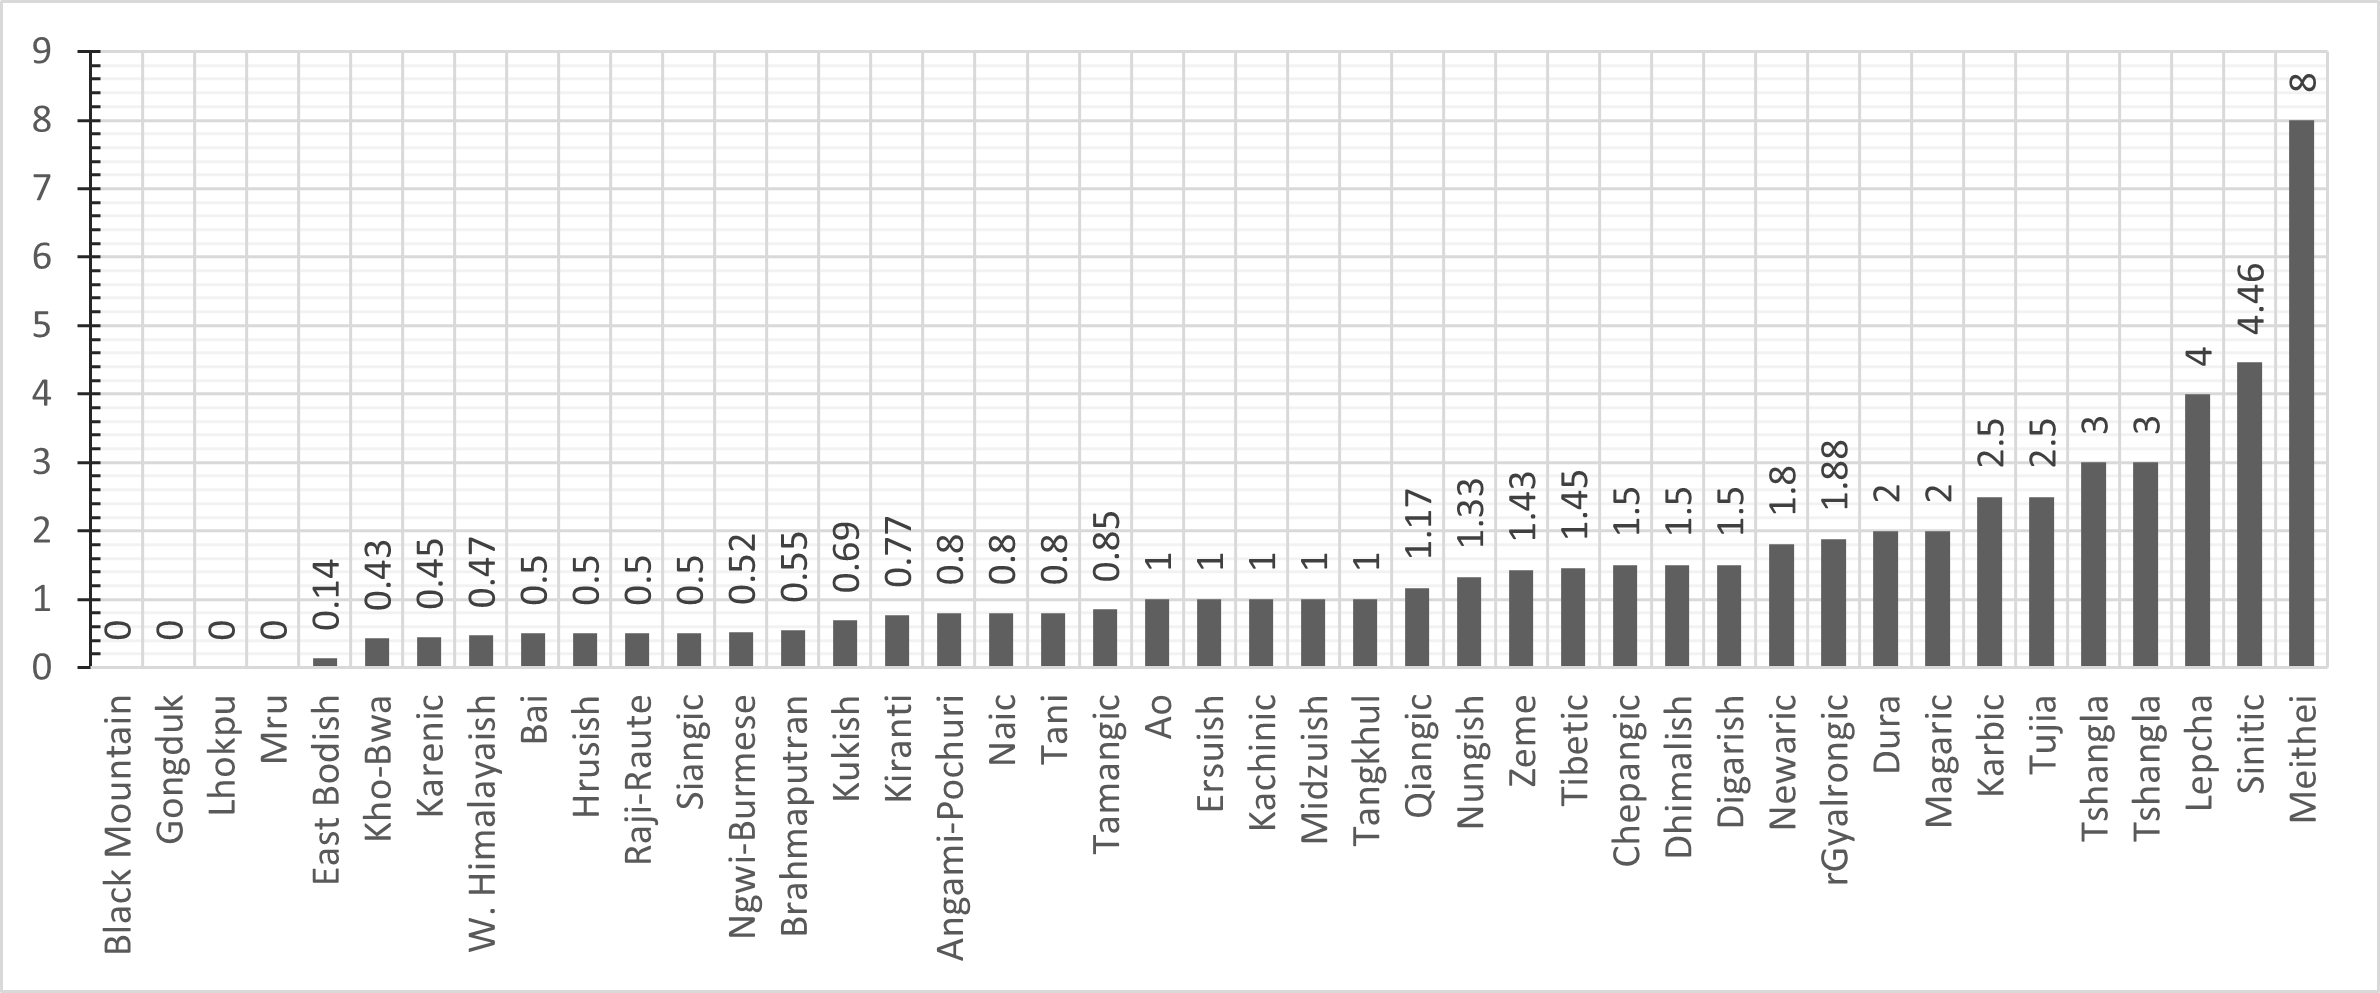
\includegraphics[scale=0.7]{Subfamily Coverage Graph.png}
        \caption{The ratio of overall grammars per language for each of the subfamilies, sorted from lowest to highest.}\label{f:Description:SubfamilyCoverageGraph}
\end{figure}

A comparison of the metalanguages of the literature in this dataset can also reveal some trends, and more specifically can reveal some gaps in the data that is available to this project, given it was limited to literature written in English with some exceptions in texts written in French or German, e.g. \citeA{Lai2017}. This data is presented in Figure \ref{f:Description:SubfamilyCoverageByLanguage}, showing the metalanguages used as a percentage of the total grammars in the dataset. Unsurprisingly, the families with higher levels of literature in Chinese, namely Bai, Digarish, Ersuish, Kho-Bwa, Mizduish, Ngwi-Burmese, Nungish, Qiangic, rGyalrongic, Sinitic, and Tujia, are all at least in part spoken in China. The Digarish, Kho-Bwa, Midzuish, and Nungish branches are all spoken partly outside of China (or in contested areas), specifically in all three cases around the tri-point between China, Myanmar, and the Indian state of Arunachal Pradesh. In these cases as well, the Chinese literature comprises one or two of a total of three or four publications. The higher level of use of French as a metalanguage in the rGyalronic subfamily (4 out of 15) can be attributed directly to the research and teaching of Guillaume Jacques, as three of the items are doctoral theses over which he was supervisor, and the final is his own grammar of Japhug \cite{Jacques2021}.

\begin{figure}
        \centering
        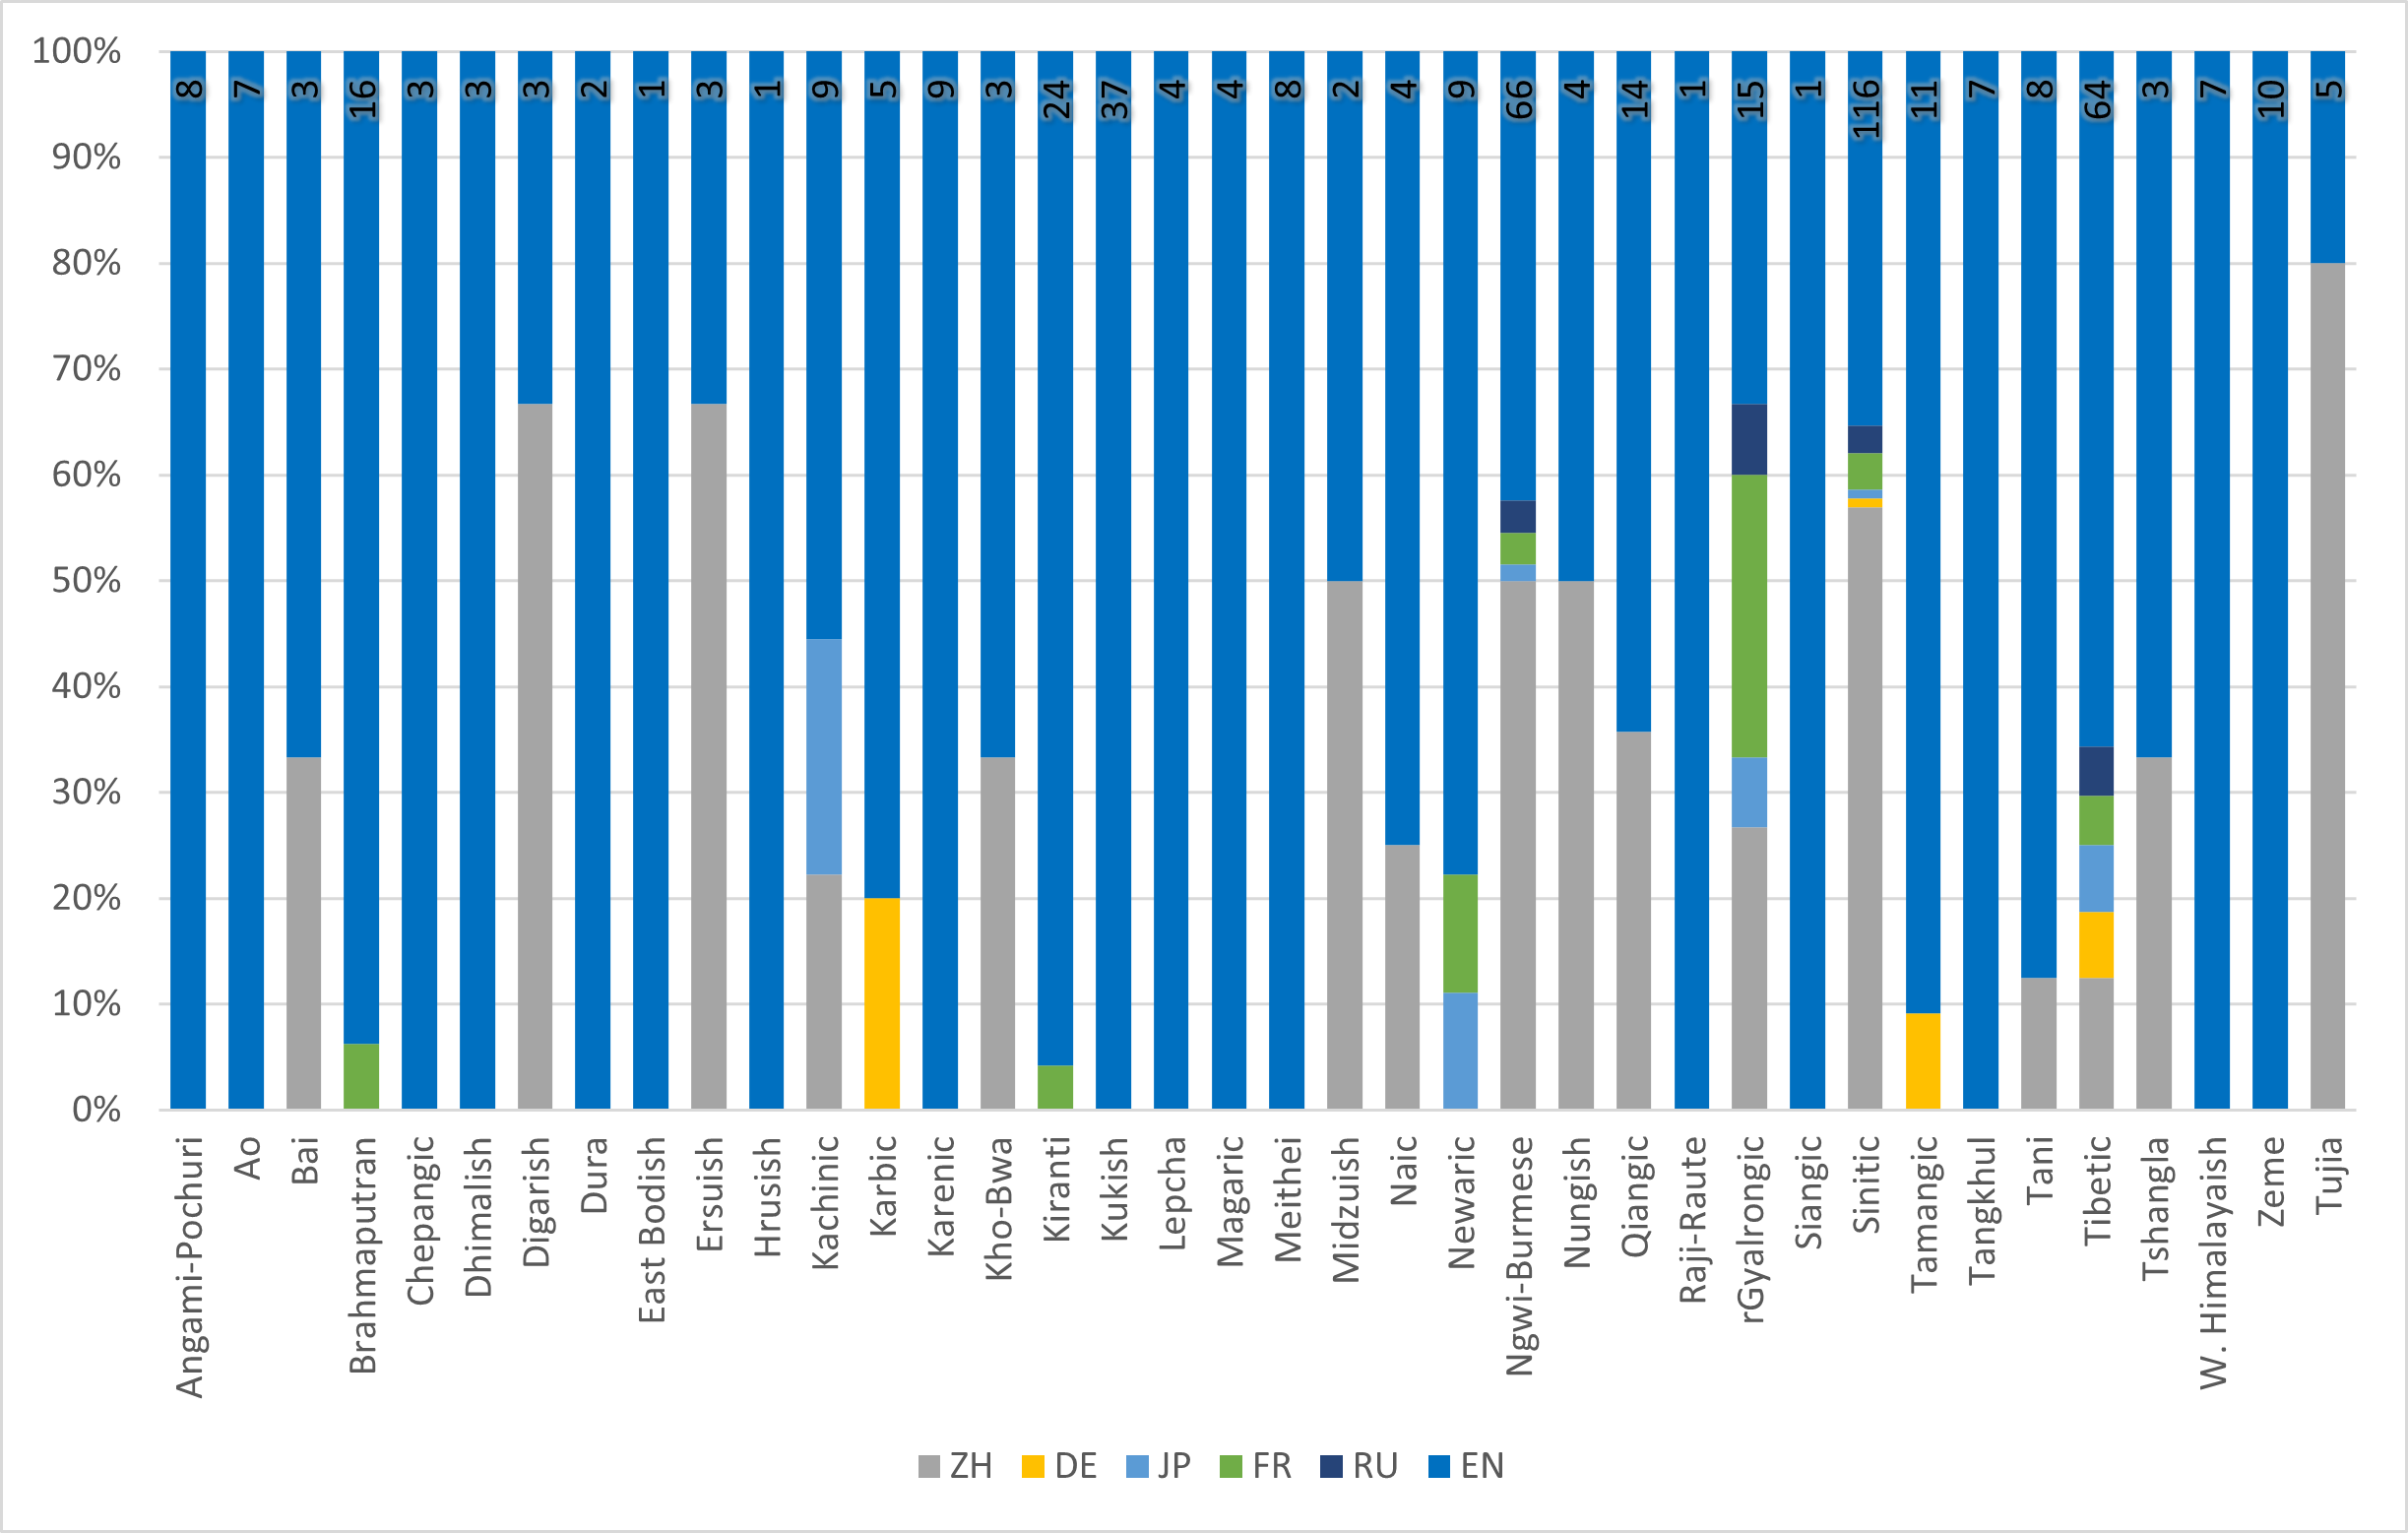
\includegraphics[scale=0.7]{Subfamily Coverage By Language.png}
        \caption{Distribution of metalanguages as a percentage of the total grammars in each subfamily. The number at the top of each subfamily is the total number of grammars in the dataset per sufamily.}\label{f:Description:SubfamilyCoverageByLanguage}
\end{figure}

Thus far, the literature being referenced in this analysis has broadly been referred to as ``published'' or as a survey of ``publications'', however it is worth noting that this also includes both masters and doctoral theses, which have not technically been published or peer reviewed in the same sense as a book would. While this is not to say that a masters or doctoral thesis is inherently less reliable than a published book, masters theses in particular are inherently shorter and less detailed. It was not feasible to annotate all of the grammars in the dataset for their initial origin in these terms, but assuming a higher number of masters and doctoral students undertaking descriptive projects than degree-holding academics undertaking such projects to the point of a published grammar, it can be assumed that theses comprise a substantial if not majority portion of the dataset\footnote{While this rings true in the current, I suspect that this has not always been the case. Additionally, the rise of theses being readily available online has made them more accessible, and potentially more common in the Glottolog database.}. To compare only the data collected for the larger analysis in this project, discussed in Section \ref{s:Methods:Collection}, about 40\% are masters or doctoral theses, and theses were generally only used where no formally published book was available.

\subsection{Languages with conflicting analyses}\label{ss:Description:Conflicts}
A challenge in taking the analyses presented in the literature at face value is that, in cases where multiple descriptions of a single langauge exist (as discussed in Section \ref{ss:Description:StateOfDescription}), there may be different, conflicting analyses of a particular form or function. This section presents a number of examples of cases where a decision had to be made, and discusses why that decision was made the way it was. 

\paragraph{Sunwar}
In his initial descriptions of mirativity, \citeA{DeLanceyMirativity1997} gives Sunwar (Kiranti: Nepal) as an example of a language showing grammaticalised mirativity. In particular, DeLancey describes the copulas \textit{tshə} and \textit{'baak-} as being distinguished based on the newness of knowledge. DeLancey reports that the use of each copula is conditioned independently of the source of the speaker's knowledge (evidentiality), but is rather conditioned by whether or not the information is known without qualification by the speaker (\textit{tshə}) or is information they have just learned, through any of reportative, inferential, or direct evidence (\textit{'baak-}). Example \ref{e:Description:SunwarMirative} shows this distinction in a minimal pair, with the non-mirative used in situations where the speaker has perhaps lived in Kathmandu and is familiar with Tangka and the mirative form used in situations where the speaker perhaps did not know Tangka was in Kathmandu but had just seen him, or had just been told he was there \cite[42]{DeLanceyMirativity1997}.

\begin{exe}
        \ex\label{e:Description:SunwarMirative}
        \begin{xlist}
                \ex 
                \gll Tangka Kathmandu-m tshaa \\
                Tangka Kathmandu-\textsc{loc} \textsc{tsha.3sg} \\
                \glt `Tangka is in Kathmandu.' (non-mirative)

                \ex
                \gll Tangka Kathmandu-m 'baâ-tə \\
                Tangka Kathmandu-\textsc{loc} exist-\textsc{3.sg.past} \\
                \glt `Tangka is in Kathmandu.' (mirative)
        \end{xlist}
        Sunwar \cite[Kiranti: Nepal,][41-42]{DeLanceyMirativity1997}
\end{exe}

\citeA{Borchers2008} disagrees with this analysis, though concedes that she and DeLancey are working with data from different Sunwar-speaking communities, and notes that DeLancey's analysis is working with a smaller corpus than hers. Borchers suggests instead that \textit{'baak-} ``is used to express the general way that things are'', whereas \textit{tshə} ``denotes the concrete and recent state of affairs'' \cite[164]{Borchers2008}. \citeA{Hill2012} is also critical of DeLancey's analysis, though in an overall argument against mirativity as valid cross-linguistic category. That being said, Hill's criticism of the mirative analysis, while referencing \citeA{Borchers2008} for support, relies only on a reanalysis of the meagre data presented in \citeA{DeLanceyMirativity1997} (here in Example \ref{e:Description:SunwarMirative}) and a discussion of edge cases one would not reasonably expect DeLancey to have discussed given the level of detail in the description given in his paper.

The question thus becomes one of which analysis to follow for this typology. That is, in order to enter data from Sunwar into the database, we must make a decision about whose analysis to follow. In this case, given Borchers, at least by her accounts, worked with substantially more data, and spent a much longer time in the field than DeLancey (who worked with a single speaker living in the United States \cite{DeLanceyMirativity1997}). This is, in all reality, a fairly minor decision. It is, in this case, a single point of data in a substantially larger database, and despite Hill's (2012) strong criticism of DeLancey's description, \citeA{Borchers2008} does give a number of possible reasons for the difference in analysis, and does not appear to go to the same length as Hill in actively attempting to refute DeLancey. There also continues to be other languages analysed as marking mirativity in the sample, and as such mirativity as a concept is still considered in this typological analysis.

\paragraph{Lhasa Tibetan}
There is a similar disagreement in the literature over the best way to analyse the evidential system in Lhasa Tibetan, again involving disagreement over the mirative between \citeA{DeLanceyMirativity1997} and \citeA{Hill2012}, though with a greater number of other possible analyses. Epistemic marking in Lhasa Tibetan varies between equative copular clauses, and existential copular, and verb clauses. Specifically, there are two epistemic bases in the equative copula system, compared to three in the existential copulas and verbal morphology \cite{DeLancey2017Tibetan}. These forms are given in Table \ref{t:Description:LhasaEpistemics}, adapted from \citeA[11]{Garrett2001} and using his labels for the 2-3 evidential bases. It is the precise labelling of these bases in a theoretical sense that has been debated in the literature.

\begin{table}
        \begin{tabular}{l|c|c|c}
         & Ego & Direct & Indirect \\ \hline
        Equative Copulas & \textit{yin} & \multicolumn{2}{c}{\textit{red}} \\
        Existential Copulas & \textit{yod} & \textit{ḥdug} & \textit{yodred} \\
        Verbal Morphology (past)\footnote{This paradigm is conditioned by both epistemics and tense/aspect. For the sake of simplicity, the past tense paradigm is given here} & \textit{-pa-yin} & \textit{-song} & \textit{-pa-red}
        \end{tabular}
        \caption{The Lhasa Tibetan epistemic system, adapted from \citeA[11]{Garrett2001}.}\label{t:Description:LhasaEpistemics}
 \end{table}

\citesA{DeLanceyMirativity1997} suggests that, in the three-base systems, the \textit{ḥdug} form represents information with an immediately accessible information source, which he analyses as mirative. As with Sunwar, \citeA{Hill2012} argues against this analysis, rather arguing that the perceived immmediacy of the evidence is a result of the actual condition for the use of the base being the presence of direct sensory evidence. This analysis of a this form as marking direct sensory evidence is also followed by \citeA{Garrett2001}, and is visible in the labelling of Table \ref{t:Description:LhasaEpistemics}. More recently, \citeA{DeLancey2017Tibetan} takes a stance between the two, suggesting that the form is conditioned by direct perception, but that (at least in some cases), this also logically suggests an immediacy of the origo's evidence that the information is also new (though not necessarily unexpected).

\citeA{DeLancey2017Tibetan} also give a different analysis of the conditions for the use of \textit{yodred} forms to \citeA{Garrett2001}. While Garrett suggests that the forms are dependent on some indirect information source, such as hearsay or inference (though this is a major simplification of Garrett's very detailed analysis of the usage of the form), DeLancey suggests an analysis in which the \textit{yodred} forms mark evidentially generic information, or information that is known without qualification or because it is simply generally known \cite[392]{DeLancey2017Tibetan}. A similar claim for a more generic factual evidential function is made for other Tibetic languages by \citeA{Zemp2020}, specifically referring to copulas. In some cases, the factual or netural function is described for the cognate of the \textit{yin} form (see also \citeA{Bodnaruk2023a}) contrasted against an evidentially marked alternative, and some cases for the form in contrast to the cognate of the \textit{yin} form, which in these latter cases marks specific speaker involvement. Zemp extends this second category to the equative copulas in Lhasa Tibetan, in which the \textit{yin} form marks personal involvement, while the \textit{red} form is evidentially neutral \cite[39]{Zemp2020}.

The distinction between \textit{yin} and \textit{red} has also been described as egophoric \cite{EgoIntro}, and does on the surface follow the expected pattern of egophoric contrasts. \citesA{Hill2017}{Gawne2017} argue against egophoricity as a separate cross-linguistic category, but rather frame it as a specific evidential base contrasted with other evidential meanings and not with a \textsc{non-ego} form that is simply defined against it. This ``egophoric evidential'' (as opposed to an egophoric marker in a theoretically distinct category) seems to generally agree with Zemp's (2021) analysis, though focusses on the 3-way distinction seen in other areas of the Lhasa Tibetan grammar. 

Unlike in Sunwar, the actual usage of the forms in Lhasa Tibetan is not in any of the literature substantially at odds. Rather, as the brief description above begins to summarise, the analyses differ in purely theoretical terms, questioning which cross-linguistic categories and theoretical frameworks and lenses best represent the well-described usage of the forms given in Table \ref{t:Description:LhasaEpistemics}. This discussion is by no means unnecessary, but is importantly not one of description per se. In fact, the clearly blurred boundaries between the categories (the 3-term system can and has been described as mirative, evidential, egophoric, and combinations of those three) begins to suggest that perhaps this siloed approach of analysis is insufficient here, a direction that \citeA{Hill2017} begin to move in, but perhaps face challenges in attempting to collapse the distinctions solely into the framework of evidentiality. Paradigms that appear to mark more than one category of epistemic marking will be further discussed in Section \ref{sss:Description:MixedSystems}, and the theoretical implications in detail in Chapter \ref{c:Discussion}.



\section{Classifications of the Data}\label{s:Description:Classifications}
This section presents a set of typological observations about the data as a precursor to the more theoretically oriented discussion in Chapter \ref{c:Discussion}. These typologies represent an attempt to categorise the data and develop an overview of the different forms and functions seen in epistemic marking across the \lfam\ family. It will also, where possible, compare these typological observations in geographic and genealogical terms. A fuller investigation into the historical implications of these trends can be found in Chapter \ref{c:History}.
\subsection{By Forms}\label{ss:Description:ClassBySystem}
There is little similarity across the language family in the forms used to mark epistemics, as would be expected given the propensity of these markers to be reanalysed and regrammaticalised from new forms (CITE). However, there are some patterns visible in the position of the markers in syntatic or morphological terms that can be seen in the data across a number of areas. Specifically, this section will describe a number of observations about the data in terms of the patterns that emerge in the forms taken by different systems. The two main patterns occur in the size of the system, which can be broadly grouped into Single Term systems and Complex systems with some subgroups, and in the scope and location of the marking, which generally either appears in dedicated morphology, copulas, or nominalisers, and can take scope over a verb phrase or verb phrase, or an entire clause.
\subsubsection{Groupings by size of system}\label{sss:Description:GroupSize}
At the highest level, epistemic systems can be categorised into two general types: Single term systems and complex systems. These systems are further each divided into two subtypes, given in Figure \ref{f:Description:SizeTypes}, and are discussed in detail below.

\begin{figure}
        \begin{itemize}
                \item Single Term Systems
                \begin{itemize}
                        \item Reportative only A3 systems
                        \item Other Single Term Systems
                \end{itemize}
                \item Complex Systems
                \begin{itemize}
                        \item Paradigmatic Systems
                        \item Scattered Systems
                \end{itemize}
        \end{itemize}
        \caption{Types of epistemic marking in \lfam\ languages per system size.}\label{f:Description:SizeTypes}
\end{figure}

Single term systems are, as the name suggests, epistemic systems that are represented by a single term or form. There are two possible theoretical interpretations of the number of epistemic bases functionally represented in these systems. First, single term systems can be viewed as just that, a single form marking specific epistemic meaning conterposed to an unmarked speech act marking no specific epistemic meaning. Alternatively, single term systems could be analysed as in fact marking two epistemic bases in opposition, with marked speech acts carrying a given epistemic meaning and unmarked speech acts explicitly carrying the opposite epistemic meaning. Perhaps a sufficient method of disambiguating between these two analyses is through obligation. If the form is obligatory in every context where its conditioning factors are fulfilled (that is, wherever it would contextually make sense), then it can be said that a speech act without said marking necessarily does not fulfil said conditioning factors, and the opposite of the form's meaning must be true.

For a hypothetical example, if a language obligatorily marks all speech acts known through reported evidence (as in, the speaker was told by someone), then, even though there is no alternative form, all statements not marked with the reportative evidential marker can be construed as reflecting the inverse of reportative evidence (any evidence other than reportative). This example is, however, hypothetical, as it is not clear from the literature available on single term systems that any such systems exist. Rather, the single term  systems in the survey are all explicitly described as non-obligatory, or it is not specified. In these actually attested cases, the fact that the marker is not obligatory in every possible usage situation means that a statement without said marking does not necessarily imply a lack of, for instance, reportative meaning. Rather, there is simply no evidential information marked. The statement could still have reportative evidence, or it could not, it is simply not at all encoded. It can be presumed that, given these forms are not necessarily used in every case where their core function is applicable, there must be some other motivational force behind their usage, though while it can be suspected that something akin to emphasis might be responsible, there is not enough discussion or description on this in the relevant literature to draw any conclusions here.

The most common type of single term system seen in the data are those marking only reportative or quotative evidence. These systems are clearly covered by Aikhenvald's (2004) typology of evidential systems, being categorised as type A3. Aikhenvald here takes the approach of presenting these systems are two term systems, with the unmarked form existing counterposed in function to the marked form, an approach against which I argue above. \citeA{Aikhenvald2004} does point out, as does \citeA{Gawne2021}, that there is an important theoretical difference between \textsc{quotative} and \textsc{reportative} evidentials which is not always represented in the literature. Here, quotative refers to markers denoting direct quotation, while reportative refers to markers denoting a reported or hearsay sourve for a given piece of information, but not present in the speech act as a direct quotation. These are, in some cases, differentiated in \lfam\ languages, an observation also made by \citeA{Gawne2021}. 
In Karbi \cite[Internal isolate: India,][]{Konnerth2020}, there are separate quotative and reportative particles. The quotative particle \textit{pu}, as is often the case \cite{Gawne2021}, is a grammaticalised and phonologically reduced (in the loss of tone) form of the verb \textit{pù}, and is used primarily in directly quoted speech, as in Example \ref{e:Description:KarbiQuot}. In addition, there is a dedicated reportative marker \textit{tànghò} used for indirect reported speech, as in Example \ref{e:Description:KarbiReport}. Notably in Karbi, the quotative \textit{pu} can also be used for indirectly reported speech, as in Example \ref{e:Description:KarbiBoth}.

\begin{exe}
        \ex 
        \begin{xlist}
                \ex\label{e:Description:KarbiQuot}
                \gll [nang=chenék-Cē pēi a-tūm] pu \\
                1/2:\textsc{nsubj}=torture-\textsc{neg} mother \textsc{poss-pl} \textsc{quot} \\
                \glt ```She won't torture you, mothers'', he said.' (p. 560)

                \ex\label{e:Description:KarbiReport}
                \gll Bēy a-tūm kortè bàng-kethòm dō tànghò \\
                \textsc{clan} \textsc{poss-pl} brother \textsc{clf:hum:pl}-three \textsc{exist} \textsc{rep} \\
                \glt `... there were three Bey brothers, they say.' (p. 562)

                \ex\label{e:Description:KarbiBoth}
                \gll a-ingjìr=tā dō pu \\
                \textsc{poss}-sister=\textsc{add} \textsc{exist} \textsc{quot} \\
                \glt `... they also had a sister, it is said.' (p. 561)
        \end{xlist}
        \cite[Karbi,][]{Konnerth2020}
\end{exe}

In cases where the quotative is descended from a verb of speech, it can be difficult to determine whether or not a form is a grammaticalised morpheme or just another use of the verb. In the case of Karbi above, the phonological reduction is a key indication that the form is actually grammaticalised. In Eastern Kayah \cite[Karenic: Myanmar,][]{Solnit1986}, however, the quotative construction is marked with a form that is identical to the verb `say'. This poses a question of how to establish whether or not a form is in fact a quotative marker that has been grammaticalised, or simply a perphrastic quotative construction involving a verbum dicendi. One possible method of distinguishing in situations where no other evidence of grammaticalisation is available (as might be the case in lanaguages with minimal morphology, such as many Ngwi-Burmese languages \todo{cite}) is to consider what range of verba dicendi are available for use in these constructions. In cases where a form has grammaticalised as a quotative marker, one might expect to only see the one verbum dicendi used in said quotative constructions, whereas in cases where the construction remains periphrastic, there might be a selection of available verbs with different meanings.

In two cases, Atong \cite[Brahmaputran: India,][]{Breugel2014} and Ersu \cite[Ersuish: PRC,][]{Zhang2013}, the quotative form appears to be in the process of being grammaticalised. In Atong, older speakers appear to mark the quotative with the verb \textit{no} `say' and the factitive enclitic \textit{=wa}, whereas the form in younger speakers appears to simply be the verb `say' used by itself as a clitic \textit{=no} in its own right \cite[408]{Breugel2014}. In Ersu, this change is visible in an analysis of the etymology of the five varied quotative markers, rather than being visible across living generations of speakers. Here, the five quotative forms are all fairly transparently derived from the verbum dicendi \textit{dʑi} `say', with various forms being used in different parts of the grammar of the language and with different scopes. This verb, while understood as meaning `say' by speakers, is marginal, and no longer used in natural speech by speakers. In this, the form \textit{dʑi} appears to have partly grammaticalised, having fallen out of usage as a verb in its own right, but not totally, as it is still understood as a verb by speakers, and the quotative constructions using it have not yet fully reified in their usage \cite{Zhang2014}.

A number of systems have also been described marking a single epistemic base other than the reportative discussed above. Some of these include other evidential bases, or mirativity. Given mirativity as a concept was excluded from \citeA{Aikhenvald2004}, no categorisation for these latter systems exists in an evidential framework. In some cases a form given is, by its description, seemingly mirative, but is not specifically termed as such in the literature. In Anong, \citeA{Sun2009} describe a series of interjections, expressing a given emotion or reaction. These forms are reported to generally occur outside the sentence. For instance, the three ``surprise markers'' \cite[111]{Sun2009} occur at the start of a speech act in the given examples, marking mirative meaning but arguably existing outside the clause entirely. 

In Western Tamang (Tamangic: Nepal), \citeA{Regmi2018} describe a mirative suffix \textit{-nyam} as part of a category otherwise marking epistemic modality. When viewed from an evidential-exclusive perspective, this marker, which is described as also having inferential evidential connotations, would be a single term, however there is a logical theoretical connection between the mirative marker and the certainty and dubiative markers alongside which it is described by \citeA{Regmi2018}. In marking information that is new or unexpected, Regmi and Regmi describe the marked information as not yet fully integrated into the speaker's knowledge structure. This can, alongside the other epistemic modal markers, be seen in terms of speaker confidence, that as well as often being inferential, the speaker is asserting less confidence over a given proposition.

Contrasted with single term systems are systems I am referring to here as \textsc{Complex Systems}. These systems, in contrast with the ambiguous or lack of oppositionally contrastive forms seen in single term systems, mark epistemic bases that are often in direct opposition to each other. These systems also fall into two subtypes, paradigmatic systems, wherein the epistemic contrasts are marked within a single paradigm or slot on the verb, and scattered systems, wherein contrasts are marked across different parts of the grammar. These scattered systems have previously been described for evidentials in great detail by \citeA{Aikhenvald2004}, and as such will not be investigated at length here.

Paradigmatic systems see the epistemic-marking system in a language contained within a single (often verbal) paradigm, occupying a single slot on the verb, comprising a set of clause-final particles, or some other set of grammatical forms. These paradigms can, however, be restricted to a specific domain of the grammar of a language, and there might be multiple paradigms across different domains. In any of these cases, the key defining feature of paradigmatic systems is that contrastive or oppositional epistemic bases are marked in formally equivalent ways. The precise definition of paradigms and paradigmatic systems is discussed in detail in Section \ref{sss:Discussion:Paradigmatic}.

The system of verbal morphology in the perfective aspect in Kurtöp \cite[East Bodish: Bhutan,][]{Hyslop2018} is an archetypal paradigmatic system of epistemic marking. There are five mutually exclusive suffixes, marking a wide variety of epistemic meanings, including mirativity, unequal epistemic authority, visual evidence, and speaker confidence. These forms all fit in the same slot after the verb, marking both perfective aspect and their given epistemic meanings. Some of these are given in Example \ref{e:Description:KurtopPerfective}, where it can be seen that the forms are representative of a single epistemic meaning selected out of a number of options.

\begin{exe}
        \ex\label{e:Description:KurtopPerfective}
        \begin{xlist}
                \ex 
                \gll ngat ge-shang \\
                1.\textsc{abs} go-\textsc{pfv.ego} \\
                \glt `I went.' (Exclusive knowledge) \cite[130]{Hyslop2018}
                \ex 
                \gll khit ge-pala \\
                3.\textsc{abs} go-\textsc{pfv} \\
                \glt `S/he went.' (Non-exclusive knowledge) \cite[130]{Hyslop2018}
                \ex 
                \gll tshe khit ge-mu \\
                \textsc{dm} 3.\textsc{abs} go-\textsc{pfv.infer} \\
                \glt `Then he left.' (Inferred) \cite[115]{Hyslop2014}
        \end{xlist}
        Kurtöp (East Bodish: Bhutan)
\end{exe}

The paradigm of existential copulas in Kurtöp is also epistemically conditioned \cite{Hyslop2014}, though the epistemic bases do not perfectly align with those in the perfective aspect, specifically in that the perfective distinction between \textit{-shang} and \textit{-pala} governed by unequal epistemic authority is not marked in the existential copulas. There is a more complete description of, and discussion about, Kurtöp verbal morphology in Section \ref{sss:Discussion:KurtopCase}.

Scattered systems are those such as in Magar, described in Section \ref{ss:Methods:MagarExample}, in which epistemic meaning for a single clause could be marked across multiple areas of the grammar of the language. This is theoretically distinct from languages with multiple paradigmatic systems as described above. In those cases, a single given clause would draw from a single paradigm occupying a single grammatical slot, even though there may be other epistemic paradigms in other areas of the language that would be used in other clauses. Here, a single clause is drawing epistemic marking from across multiple areas of grammar at once. In the case of Magar, a single clause might have mirative marking in the form of a nominalised construction, inferential marking in the orm of a verb suffix, reportative marking in the form of a particle, or unmarked direct visual evidence. These are shown in Examples \ref{e:Methods:MagarMirativeIntro} and \ref{e:Methods:MagarEvidIntro}, and again in \ref{e:Description:MagarScattered} for convenience. A minimal set of all forms was not available in the publications, so a second unmarked, direct example has been given in \ref{e:Description:MagarScattered:d} for the sake of comparison with its mirative form in \ref{e:Description:MagarScattered:e}

\begin{exe}
        \ex Evidential Contrasts\label{e:Description:MagarScattered}
        \begin{xlist}
          \ex Direct (Unmarked)
          \gll ho-se taɦ-raɦ-a \\
          \textsc{d.dem-def} reach-come-\textsc{pst} \\
          \glt `He has arrived.' (I see him.)
      
          \ex Inferential (Verbal morphology)
          \gll ho-se taɦ-raɦ-le-sa-a \\
          \textsc{d.dem-def} reach-come-\textsc{-impf-infr-pst} \\
          \glt `He has arrived.' (I see his bag.)
      
          \ex Reportative (Particle)
          \gll ho-se taɦ-raɦ-a ta \\
          \textsc{d.dem-def} reach-come-\textsc{pst} \textsc{rep} \\
          \glt `He has arrived.' (They say.)

          \ex Non-mirative, Direct (Unmarked) \label{e:Description:MagarScattered:d}
          \gll thapa i-laŋ le \\
          Thapa \textsc{p.dem-loc} \textsc{cop} \\
          \glt `Thapa is here.'
      
          \ex Mirative (Nominalisation)\label{e:Description:MagarScattered:e}
          \gll thapa i-laŋ le-o le \\
          Thapa \textsc{p.dem-loc} \textsc{cop-hab} \textsc{impf} \\
          \glt `(I realize to my surprise that) Thapa is here!' 
        \end{xlist}
        Magar \cite[Magaric: Nepal,][480, 497]{GrunowHarsta2008}
      \end{exe}

Languages can show a mix of paradigmatic and scattered systems, including in a single grammatical domain. This is to say that one might see a paradigmatic system of epistemic marking in, for instance, the copulas of a language, and a scattered system in some part of the verbal morphology.\todo{example} One might also see a partially paradigmatic system of epistemic marking, with some epistemic bases marked by forms occupying the same grammatical slot and others marked in other areas of the grammar.\todo{example}

\subsubsection{Groupings by Scope and Position}\label{sss:Description:ScopePosition}
\citeA{GrunowHarsta2008} notes, citing \citeA{Noonan2008}, a tendency for mirative marking to take the form of nominalisation in the Central and Western Himalayan region, contrasted with the use of copulas in ``Bodish''\footnote{This is given in quotes as it is not necessarily clear without further disambiguation what this term means. Here, it appears to include Suwnar (Kiranti: Nepal), suggesting a very broad use of the term.} (p. 480) languages. This contrast can be extended with the inclusion of otherwise non-contrastive morphology to cover much of the family, as well as to cover epistemic marking more broadly. That is, epistemic marking overall tends to either appear in \lfam\ languages in the form of nominalisations, copulas, or as dedicated morphology. As can be seen in Example \ref{e:Description:MagarScattered}, a single language can also exhibit all of these across a system, as well as, to be discussed below, in single forms. Dedicated morphology too, can take multiple forms. Differentiated from nominalisers as they have no derivational function, dedicated morphology can take scope over a verb or a full clause. This is to say that in some cases, forms are marked directly on the verb or as particles with clear scope over a verb phrase, whereas in others, forms are marked as clause-final particles or enclitics with scope over the entire clause. In any of these cases, forms are purely inflectional, and do not have the derivational component of the nominalisers.

A different case of nominalisations playing a role in epistemic marking can be seen in Milang \cite[Siangic: India,][]{Modi2017}, in which all basic clauses and finite verbs reflect an egophoric meaning or claim over epistemic authority unless neutralised by a nominalisation construction. In this case, the nominaliser could be analysed as carrying a specific non-egophoric meaning, though \citeA{Modi2017} rather analyses the construction as a neutralisation of a meaning that is inherent in clauses with finite verbs, rather than any meaning marked by a specific piece of morphology in any case.

Copulas marking epistemic contrasts are particularly common across the Tibetic subfamily \cite{Zemp2020}, though can be found in other languages with substantial contact with Tibetic languages (e.g., East Bodish languages such as Kurtöp \cite{Hyslop2020Kurtop} and Tawang Monpa \cite{Tombleson2020}, West Himalayish languages such as Chhitkul-Rakchham \cite{Martinez2021}), as well as Lhokpu (likely Dhimalish: Bhutan), which has potentially had significant contact with Dzongkha, though no influence has yet been proven at this point in time. An epistemic distinction in copulas can also be seen in Duhumbi \cite[Duhumbi: Kho-Bwa,][]{Bodt2020}, a language which does not have any direct contact with Tibetic languages due to a buffer of Tshangla and East Bodish langauges to its North and West.

In a number of Tibetic languages in particular, a combination of nominalisers and copulas has been grammaticalised into verbal morphology. A set of these forms in Lhasa Tibetan are given in Table \ref{t:Description:LhasaTibetanFinite}. The nominalisers \textit{-ki} and \textit{-pa} are used in conjunction with epistemically contrastive copulas to form finite verb suffixes. Interestingly, the tense/aspectual meaning is not only encoded by the choice of nominaliser, but also the set of copulas used. That is, the perfective (or simple past in \citeA{Garrett2001}), aside from the direct form \textit{-song} which does not follow this pattern but rather uses a grammaticalised form of a verb of motion, uses the equative copulas and the nominaliser \textit{-pa}, while the future uses the equative copulas instead with the nominaliser \textit{-ki}. In both cases, the direct form is either formally separate or missing, as the Lhasa Tibetan equative copulas only exhibit a two-way contrast. The imperfective aspect on the other hand shares the nominaliser \textit{-ki} with the future forms, but uses the three-term system of the existential copulas \textit{yod, ḥdug} and \textit{yodred}. Here, the nominalisers themselves do not carry the epistemic meaning, but serve, at least diachronically, as a means for the attachment of the epistemically contrastive copulas onto the verb, and synchronically also mark other parts of the tense/aspect system. This does not on the surface appear to be a similar process by which one might imagine the systems in which nominalisers also carry epistemic meaning. This can be seen in a comparison of the Lhasa Tibetan paradigm given in Table \ref{t:Description:LhasaTibetanFinite} and Example \ref{e:Description:MeitheiNominaliser} from Meithei \cite[Internal Isolate: India,][296]{Chelliah1997}, in which a similar construction of nominaliser-copula can be seen. While in Lhasa Tibetan, the copulas carry epistemic meaning in isolation and continue to do so when further grammaticalised into a verbal paradigm, in Meithei it is the nominaliser \textit{-ǰat}, glossed by \citeA{Chelliah1997} as \textsc{type}, which carries the epistemic meaning of inferential evidence, and carries such meaning when not followed by a copula. As such, not all nominalisers used in association with epistemically contrastive forms are necessarily themselves epistemically contrastive, and as such, while the Meithei form of \textit{-ǰat} would be classified as a nominaliser-type epistemic marking, the Lhasa Tibetan nominalisers \textit{-ki} and \textit{-pa} would not be treated in such a typology at all, as they do not on their own encode epistemic meaning. It is possible that the epistemically contrastive nominalisers did develop diachronically through a pathway that at one point looked similar to the system in Lhasa Tibetan, and in fact \citeA{DeLancey2017Tibetan} does note that the copula component of the direct imperfective suffix \textit{-ki-ḥdug} is regularly omitted in speech. That being said, the possible diachronic origins for the epistemic nominaliser forms, or the potential future development of the Lhasa Tibetan forms, while an interesting question worth further consideration, are not necessarily so relevant for a synchronic typological overview of the systems and fall outside the scope of this project. 

\begin{table}
        \begin{tabular}{l|c|c|c}
         & perfective       & imperfective         & future           \\ \hline
        ego                  & \textit{-pa-yin} & \textit{-ki-yod}     & \textit{-ki-yin} \\
        direct               & \textit{-song}   & \textit{-ki-ḥdug}    & \textit{}        \\
        indirect             & \textit{-pa-red} & \textit{-ki-yodred} & \textit{-ki-red}
        \end{tabular}
        \caption{Lhasa Tibetan finite verb suffixes by tense/aspectual and epistemic meaning, adapted from \citesA{DeLancey2017Tibetan}{Garrett2001}.}\label{t:Description:LhasaTibetanFinite}
\end{table}

\begin{exe}
        \ex\label{e:Description:MeitheiNominaliser}
        \glll məsi phúrə́beǰatni \\
        mə-si phú-lə́bə-\textbf{ǰat}-ni \\
        \textsc{nm-pdet} beat-\textsc{having-\textbf{type}-cop} \\
        \glt `It looks like it might have been beaten' \\
        \cite[Meithei,][296]{Chelliah1997}
\end{exe}

\subsection{By Functions}\label{ss:Description:ClassByFunction}
While the above categorisations focussed on differences in the forms of systems, that is, the morphological or syntactic descriptions of systems, this section will focus on functional differences, or differences in semantic or pragmatic content. Function can be construed in two ways, which are in effect the same but can provide a different theoretical perspective. One is to discuss functions of foms in a system as carrying a given meaning, and speakers select a form based on this meaning. Given the inherent deictic nature of epistemic marking, however, it can also be helpful to view forms as having their usage determined by a series of conditions, which are assessed by the speaker during speech. In essence, on one hand, forms can be viewed as carrying their meaning inherently, or rather being made up of a series of conditions or criteria informing their usage. These two views of function are by no means mutually exclusive, nor are they in reality particularly different, but they do provide two alternative methods for explaining and analysing functions of forms in epistemic systems, and of systems as a whole. Both will be used in this section, and in Chapter \ref{c:Discussion} for the sake of clarity in explanation.

This section will present three typological observations of the functions of epistemic systems. Firstly, Section \ref{sss:Description:MixedSystems} discusses variation in the breadth of functions marked within an epistemic system. Section \ref{sss:Description:SpeakerNonSpeaker} presents a cline of functions in terms of their closeness in terms of authority to the epistemic origo, and Section \ref{sss:Description:AddrPersp} discusses variation in the presence of markings which reflect the persective of the addressee across interrogative and declarative constructions.

\subsubsection{Groupings by breadth of functions}\label{sss:Description:MixedSystems}
An ongoing challenge in the literature is the analysis of epistemic systems which mark functions that would traditionally be divided across multiple categories. This is contrasted with systems that fit into a single category such as evidentiality or egophoricity. These Mixed Systems, which will be described here in formal terms and discussed in greater detail in more theoretical terms in Chapter \ref{c:Discussion}, are, by definition, a subset of the complex systems discussed in Section \ref{sss:GroupSize}, as they are necessarily made up of multiple terms. Mixed systems can be seen in the paradigmatic systems also described in Section \ref{sss:GroupSize}, with Kurtöp being something of an archetypal example, marking meanings that would fall across evidentiality, egophoricity, engagement, and mirativity \cite{Hyslop2020Kurtop}. Another such system is found in Eastern Geshiza. \todo{exemplify?}

There is a valid question regarding these mixed systems as to whether an alternative system marking only epistemic meanings from a single category exists. There are a number of potential arguments against this. Firstly, there is often an inherent connection between evidential meaning and epistemic modal meaning \cite{Boye2012}, in which forms marking worse evidence (inferential as opposed to visual) also carry a lower level of epistemic support. Such systems can still be described in terms of evidentiality, however, and the epistemic modal meanings can be treated as secondary, as argued by \citeA{Aikhenvald2004}, if the epistemic modal is taken as a little more than an inherent logical result of evidential meaning. There is a argument in \citeA{Hill2012} that DeLancey's (1997) analysis of the Lhasa Tibetan existential copula \textit{ḥdug} as mirative is better explained as a direct visual evidential, with the mirative meaning being similarly explained as a logical result of the often immediate nature of the information being represented. In these senses, many epistemic forms can be analysed as marking other epistemic meanings as secondary or logically implied. The systems described here as mixed systems refer more specifically then to systems in which these cross-categorical functions occur on different forms, as seen in, for example, Kurtöp and Eastern Geshiza, as opposed to as secondary or potentially logically predictable meanings of a single form.

Contrasted with these mixed systems are systems which, when considering only primary meanings and not the logically resultant secondary meanings discussed above, are systems which clearly fit into a single category. These would be systems such as the commonly cited egophoric distinction in Kathmandu Newar, or the evidential system in Lhasa Tibetan as per the analysis by \citeA{Gawne2020}, in which the egophoric or participatory base is analysed as a form of evidential. In both of these cases, however, it must be considered whether or not this egophoric-only or evidential-only label is necessarily the most accurate, or if, separate to logically resultant secondary meanings, there are other factors conditioning the use of the forms that would cause challenges for an analysis of the system solely within the framkework of a single category. 

As will be discussed in Chapter \ref{c:Discussion}, in many languages, even where a system appears on the surface to be conditioned by a single category, the selection of epistemic forms is also informed by some other often social factor. For instance in Lhasa Tibetan, the ego evidential base can also be used with information that was not directly experienced by the speaker but by close relations such as family members \cite{Tournadre2008}, meaning that the speaker's relationship with the agent of the sentence is also a relevant consideration. Similarly, the use of the two egophoric bases in Kathmandu Newar, or of a potential third egophorically unmarked form, might be conditioned by the social status of speaker and addressee in relation to each other \cite{SinghShrestha2023}. These alternative or extra factors conditioning the use of these forms are potentially distinct from the secondary meanings discussed above, in that they are not logically resultant from the primary meaning. That is, assuming the lower epistemic support (in terms of epistemic modality) of forms with weaker evidence as argued by \citeA{Boye2012} is not a conditioning factor in the use of the form but is a logical implication that can be drawn from the primary meaning, whereas the use of egophoric marking when referencing, as in Lhasa Tibetan or Kathmandu Newar, the experiences of close relations or the use of non-egophorics when referencing the experiences of people of lower social status and the additional meaning this adds to the egophoric or non-egophoric markers is not a logical implication inherent to the primary meaning of the form. A test to distinguish these two, perhaps, is whether or not this additional meaning would break the condition of the primary meaning. In the case of the egophoric marking discussed, the forms are able to be used outside the more commonly cited conditions for egophoric marking given these additional conditions - they break the basic conditions and are as such additional primary meanings or conditioning factors in the use of a form. The lower support of inferential evidence however, is not a meaning outside the canonical use of inferential evidentials, and is as such not a separate conditioning factor in the use of the form.

In any case, this distinction between mixed and single category systems is arguably purely present in theoretical terms. A system can only mark functions across theoretical boundaries if those theoretical boundaries have been drawn such that a system crosses them. As can be seen from the wide variation in analyses and the lively discussions in the literature on the boundaries between categories as discussed in Chapter \ref{c:Literature} (e.g. \citesA{DeLancey2012}{HengeveldOlbertz2012}{Hill2012}{Hill2020} among others), the way in which these boundaries are drawn is not arbitrary, but is certainly open to varied interpretation. As such, the existence of a contrast between systems which mark functions only in one traditionally described category as opposed to systems which mark functions across multiple categories is dependent on the boundaries as they have been drawn. This argument largely relies on an assumption, however, that these traditional categories do only exist in theoretical terms. That is, this idea that a distinction between intra- and inter-category systems is purely theoretical as it is dependent on the theoretical boundaries drawn to form said categories is not valid if the categories and their boundaries are not purely theoretical, but exist somehow in more concrete terms beyond the analysis of a linguist. The widespread existence, however, of solely ``evidential'' systems, among others, suggests that there is a real typological justification for these categories, but, as will be argued in greater detail in Chapter \ref{c:Discussion}, this does not extend to every system marking evidential-type distinctions.

\todo{I remember reading about a language wher the mirative also had low epistemic support meaning but i forget where now}


\todo{inc. vs exc. EM?}

\subsubsection{\textsc{Speaker}/\textsc{Non-speaker} contrasts}\label{sss:Description:SpeakerNonSpeaker}

A common feature of epistemic marking across the Himalayas is a contrast between a higher level of personal involvement and a lower form. This has been observed previously by \todo{cite evid volume intro}, who noted a number of common equipollent distinctions in which forms are defined against each other. Here, I propose that many of these forms, even when not initially defined as egophoric or relating to speaker authority, can be analysed as marking a very general \textsc{speaker}/\textsc{non-speaker} contrast. That is, while the boundaries of \textsc{speaker} and \textsc{non-speaker} and conditions by which they are assessed are widely varied, many of the epistemic-marking systems surveyed in this project can be seen as fundamentally contrasting between knowledge closer to the speaker in some way, or further from the speaker. Similar observations have been made previously about the functions of evidential marking in use with reference primarily to languages spoken in South America by \citeA{Bergqvist2023}, who note that more recent descriptive projects on evidential marking have found that they often mark ``ownership of knowledge'' as opposed to the traditional definition of ``information source'' (p. 2). Commonly observed conditions for this contrast are given below. 

\begin{enumerate}
        \item Speaker authority
        \item Speaker volition
        \item Speaker evidence
\end{enumerate} 

The terminology presented here is by no means perfect, and it bears acknowledging that the \textsc{speaker} form is not necessarily always aligned with the speaker themself, but rather can be aligned with the evidential origo. While in declarative utterances this is an unnecessarily specific distinction to make, in interrogative utterances, many languages shift the origo to the addressee, and as such, the forms here described with the \textsc{speaker} label would actually be marking a higher level of epistemic authority on the part of said addressee. This origo-shift is discussed in greater detail in Chapter \ref{c:Discussion}, but is not totally consistent across all languages, nor across all forms within languages. 

While some \textsc{speaker}/\textsc{non-speaker} distinctions appear in binary or equipollent opposition (either the speaker has authority or the speaker does not), others appear as a scale from closest to the speaker in epistemic terms to furthest away. In these scalar contrasts, there can be a larger number of more fine-grained epistemic bases marked, with conditions on their use varying widely and often covering multiple traditional cross-linguistic categories. Across these \textsc{speaker}/\textsc{non-speaker} distinctions, there appears to be a tendency for the \textsc{speaker} form (or, closest form in scalar systems) to be less marked or unmarked\todo{provide evidence}. This is in line with \citeA{Garrett2001}, who argues with regards to Lhasa Tibetan that the egophoric base (the most \textsc{speaker} form in the epistemic system) is the most general form, and that the other, \textsc{non-speaker} forms are more specified. While all forms in Lhasa Tibetan are formally marked, it follows that, were one form to be unmarked, it would be the most general. With this analysis and the general observation that \textsc{speaker} forms are more likely to be unmarked (out of the available epistemic bases, where any form is unmarked), the conclusion of a default \textsc{speaker} interpretation of communication when no further clarification is provided can be more broadly extended. Such a default assumption is also explicit in Milang, as well as potentially in Galo, both discussed below.

\paragraph{Speaker authority}
To an extent, all the contrasts discussed here are conditioned by some assessment of speaker (or, more specifically origo) authority, though here I specifically refer to contrasts that appear to be conditioned solely by an assessment of epistemic authority by a speaker without reference to the specific source of said authority.
Milang \cite[Siangic: India,][]{Modi2017} exhibits an equipollent \textsc{speaker}/\textsc{non-speaker} distinction at a much more fundamental level than is seen in many other languages, in that all unmarked predicates are speaker-authority in function. That is, speaker-authority is taken as a default for all unmarked predicates, and in order to communicate non-speaker-authority, the predicate must be nominalised in order to neutralise this inherent speaker-authority \cite[455]{Modi2017}. Modi uses the term \textsc{egophoric} to refer to this, though I avoid that term here as the distribution of the speaker-authority forms is much wider than the standard distribution of egophorics as discussed in Section \ref{}\todo{The section defining egophoricity}, for example, while \exref{e:Description:MilangEgo1} would fit into the common narrow definition of egophoricity, \exref{e:Description:MilangEgo2}, in which the speaker is claiming epistemic authority over an event in which they are not the subject (or, for that matter, at all involved), would not.

\begin{exe}
        \ex\label{e:Description:MilangEgo}
        \begin{xlist}
        \ex \label{e:Description:MilangEgo1}
        \glll ŋa tutu. \\
        ŋa tu-tu \\
         1.\textsc{sg} eat-\textsc{pfv} \\
         \glt `I ate.' \\
         \cite[Milang,][455]{Modi2017}

        \ex \label{e:Description:MilangEgo2}
        \glll joon bozar yitu. \\
        joon bozar yi-tu \\
        John market go-\textsc{pfv} \\
        \glt `John went to the market' \\
        \cite[Milang,][456]{Modi2017}
        \end{xlist}
        
\end{exe}

Modi notes that this speaker-authority meaning even in non-first-person clauses is visible in two ways, through pragmatic and social restrictions, as well as through opposition with the non-speaker-authority constructions to be presented below. In pragmatic terms, a statement such as in \exref{e:Description:MilangEgo2} implies a direct knowledge on the part of the speaker, and, Modi reports, it would be considered improper, if not directly very rude, to question this knowledge (e.g., asking `How do you know?') (Modi p.c.). Simply by using the unmarked predicate structure, a speaker is claiming clear epistemic authority over an event to the extent that it ought not even be questioned.

If a speaker did not have grounds to make this claim, however, they must neutralise this speaker-authority function through the use of a nominaliser and a particle, as in \exref{e:Description:MilangNonEgo}. Here, the nominaliser \textit{ɲi} is followed by a particle \textit{la} or \textit{pɨ}, with reportative evidential or low epistemic support functions respectively.

\begin{exe}
        \ex \label{e:Description:MilangNonEgo}
        \glll joon bozar yituɲila | yituɲipɨ \\
        joon bozar yi-tu-ɲi-la | yi-tu-ɲi-pɨ \\
        John market go-\textsc{pfv}-\textsc{nzr:subj}-\textsc{rep} | go-\textsc{pfv}-\textsc{nzr:subj}-\textsc{ucrt} \\
        \glt `John went to the market. (I am told) | (I am not sure)' \\
        \cite[Milang,][457, given as two examples in source and combined here]{Modi2017}
\end{exe}
As in many cases where a \textsc{speaker}/\textsc{non-speaker} distinction can be seen, there are further epistemic meanings that can be marked in Milang using particles after the nominaliser. Two forms are given in \exref{e:Description:MilangNonEgo}, though there are many more, carrying various meanings that could be interpreted as epistemic (e.g. ignorance, strong assertions, inferential evidence) \cite[273]{Modi2017}.

A similar situation might exist in Galo (Tani: India), in which speakers reported an expectation that in sentences unmarked for evidentials the speaker ``must be `absolutely sure' of the information represented'', though it is not totally clear if this is a function of the construction as in Milang or just a logical result of the unspecified evidential component \cite[112]{Post2013}. That said, outside of this possible speaker-authority meaning, other domains of the language's grammar do exhibit unambiguous egophoric marking. These unambiguous egophoric markers show a similar condition on their use as the Milang data, in that they are also conditioned by an assessment of speaker authority rather than speaker volition. That is, while they are much closer to canonical egophorics in their restriction to first-person declaratives and second-person interrogatives, cases where a speaker has no volition over an action are still marked as speaker-authority. \exref{e:Description:GaloNonVolition} demonstrates this, in which a report that the speaker fell from a balcony (specifically without meaning to, and likely even directly against their intentions) still uses the egophoric affix \textit{tó} as opposed to the inverse \textit{gée}, labelled \textsc{alterphoric} by \citeA{Post2013}.

\begin{exe}
        \ex \label{e:Description:GaloNonVolition}
        \glll ŋó koodâa tokkə̀ {olôo tobá} \\
        \textbf{ŋó} koodâa tokkə̀ ò-lòo-\textbf{tó}-bá \\
        \textbf{\textsc{1sg}} balcony \textsc{abl.up} fall.from.height-\textsc{downward}-\textsc{\textbf{ego}}-\textsc{pfv:dir} \\
        \glt `I fell from the balcony (I know, I experienced it).' \cite[Galo,][123, emphasis from source]{Post2013}
\end{exe}

Post also gives being hungry as an example of a non-volitional event still marked egophoric, or \textsc{speaker}, in first person.

Both Galo and Milang show forms that are described in their sources as egophoric, and both are, in their function, reasonably close to the definition given in Chapter \ref{c:HimalayanBackground}. In addition to these, there are other forms that can be considered conditioned by speaker authority that fall further from the definition of egophorics.

\todo{data here, ideally not just geshiza}

Even within this group of authority-conditioned contrasts, there is a large variation in the exact boundaries of these conditions, as is visible in the two examples given above. In Milang, speaker authority can extend to third-person statements. The speaker needs visual evidence, and presumably needs a higher level of authority than the listener\todo{check this, with yankee?}, but can claim epistemic authority even if they did not directly experience it. In Galo on the other hand, while the claiming of epistemic authority is not conditioned by volition, it is still limited to first-person experience.

There are yet further ways that lines of distinction can be drawn, including with partial reference to volition. Some dialects of Amdo Tibetan combine both volitional and some non-volitional events into the single \textsc{speaker} form \cite{Tribur2019}. \citeA{Tribur2019} specifically gives the following two criteria for the use of the ego form in the Gcig.Sgril (rNgaba) variety: either that the speaker was a ``controlling and volitional participant'' in the event \cite[383]{Tribur2019}, or that the speaker was directly affected by the event and they were aware of it for its entire duration. Similarly, for copulative clauses, non-volitional authority can be claimed where there is a suitable level of social proximity from the speaker to the subject, though the acceptability of these forms conditioned by social authority can vary from village to village \cite[213]{Tribur2019}. These forms will be discussed further in Chapter \ref{c:Discussion}.

\paragraph{Speaker volition}
The primary egophoric base in Lhasa Tibetan is, on the other hand, restricted to situations where the speaker had direct volition over the first-person event. Compare \exref{e:Description:GaloNonVolition} with \exref{e:Description:LhasaVolition} below. The egophoric form is disallowed, or, as noted by \citeA{Garrett2001}, can be interpreted with the alternative meaning `I will pretend to be sick'.

\begin{exe}
        \ex \label{e:Description:LhasaVolition}
        \gll * sang.nyin nga na-gi-yin \\
        {} tomorrow \textsc{1.sg} sick-\textsc{fut}-\textsc{ego} \\
        \glt `Tomorrow I will be sick.' \cite[Lhasa Tibetan,][164]{Garrett2001}
\end{exe}

Lhasa Tibetan does not, however, treat non-volitional first-person actions as equal to events for which the speaker has observed evidence, but rather in the perfective aspect introduces a distinction between the primary egophoric base given above, for first-person agents, and a separate form for first-person patients and experiencers. That is, the \textsc{speaker}/\textsc{non-speaker} distinction is more finely divided than in Galo and Milang above. A correct form of \exref{e:Description:LhasaVolition} (though in the perfective) is given in \exref{e:Description:LhasaEgoErgExperiencer}, in which the suffix \textit{-byung} marks the first-person experiencer. In \exref{e:Description:LhasaEgoAbsExperiencer}, the breadth of this experiencer category is shown, in that \textit{-byung} can also be used with first-person patients, as the speaker still has first-hand interior knowledge of the event and claim epistemic authority thereby, but to a lesser extent than if they were a volitional agent.

\begin{exe}
        \ex
        \begin{xlist}
                \ex\label{e:Description:LhasaEgoErgExperiencer}
                \gll khasa nga na-byung \\
                yesterday \textsc{1.sg} sick-\textsc{pfv.exp.ego} \\
                \glt `Yesterday I got sick.' \cite[Lhasa Tibetan,][169]{Garrett2001}

                \ex\label{e:Description:LhasaEgoAbsExperiencer}
                \gll kho-s nga-r gzhus-byung \\
                \textsc{3.sg-erg} \textsc{1.sg-dat} hit-\textsc{pvf.exp.ego} \\
                \glt `He hit me.' \cite[Lhasa Tibetan,][395]{DeLancey2017Tibetan}
        \end{xlist}
\end{exe}

Gawne presents a number of examples of cognates of this form with similar functions  in a number of Tibetic languages \citeA[66]{Gawne2017}, as well as outside the Himalayas, but does not mention any non-Tibetic \lfam\ languages with this marking. Over the course of this study, I have also not identified any non-Tibetic languages with this marking.

\citeA{Simon2021} reports in the Rebkong variety of Amdo Tibetan a different condition separating speaker-volition forms from non-speaker-volition. Unlike in the rNgaba variety, discussed above, cases in which the speaker has a claim of epistemic support without direct involvement have a separate form, labelled as the \textsc{ego-authoritative} \cite[300]{Simon2021}. This is separate from the Lhasa Tibetan distinction above in that it does not require any participation from the speaker in the statement, agent, patient, or otherwise, but does require a social position to claim said authority, more similar to the \textsc{speaker} form in Milang.

\paragraph{Speaker evidence}
Speaker evidence conditions the selection of epistemic marking in many, if not most, of the languages with epistemic marking in the survey. This, of course, is not a surprise, as evidential marking is both widespread and widely studied across the Himalayas. This section will present these conditions (that is, evidential marking) as a criterion by which a speaker can claim authority (or a lack thereof) over a statement. In opposition to the distinctions discussed above, in which the use of a \textsc{speaker} form is condition by a general claim of authority, by specific volition, or by some combination of those two, these evidential systems can be viewed in the same framework as being conditioned by speaker evidence. Following the typology of system complexity and size discussed in Section \ref{ss:Description:ClassBySystem}, there is a large number of A3 system across the \lfam\ family, and yet more considering that some languages with complex evidential systems such as Lisu \cite{Bradley2002} and Akha \cite{Thurgood1986} can be reconstructed or traced back to A3 systems. These are in contrast to the more complex systems with multiple epistemic bases. These A3 systems will be dealt with separately here as they pose a number considerations to this proposed typology that are worth considering specifically. 

While the conditions discussed above, authority and volition, have been presented primarily in binary terms, many systems conditioned by evidence have more distinctions and forms, and will be presented here as marking a scalar \textsc{speaker}/\textsc{non-speaker}, in which various types of evidence can be seen as more or less authoritative. In most cases, this scale is theoretically clear: visual evidence is the strongest, and sees the speaker claiming the most authority over evidence, and indirect evidence such as inference and hearsay is further from the \textsc{speaker}. Languages which also mark an egophoric base, sometimes presented as conditioned by speaker evidence in \lfam\ languages \cite{Hill2017}, as well as in other parts of the world such as Papua New Guinea \cite{SanRoque2012}, would see this base as closer to the \textsc{speaker} end of the scale. The tendency for \textsc{speaker} forms to be unmarked is further supported here, as cross-linguistically visual evidentials are more likely to be unmarked than evidentials with less epistemic authority \cite[73]{Aikhenvald2004}. Aikhenvald does not factor egophoric evidentials into this typology however, as she treats them separately to evidentiality.

The placement of inferential and reportative evidence in systems where they are distinguished along this scale is not as immediately clear. \todo{more here}

This scale is supported by the wider literature in a number of additional ways. There is a common link between speaker confidence or certainty (epistemic modality) and speaker evidence (evidentiality), dicussed in detail by \citeA{Boye2012}, who draws a typological connection between ``direct justification'' (direct evidence) and ``full support'', as well as between ``indirect justification'' and ``partial support''(p.130). Similarly, \citeA{Gawne2021} notes that reportative evidentials in the \lfam\ family often work to weaken a speaker's claim of authority. This crossover is also exemplified throughout the descriptive literature. For example, in Dhimal \cite[Dhimalish: India,][245]{King2009} the \textsc{deductive} particle \textit{wa} carries a meaning of both inferential evidence, as well as low epistemic commitment by the speaker. In \exref{e:Description:DhimalDeductive}, the speaker avoids claiming authority over the presented, rather suggesting that while they have some reason to believe that someone does not understand, the opposite is also still possible.

\begin{exe}
        \ex\label{e:Description:DhimalDeductive}
        \gll ma-gi-khe wa \\
        \textsc{neg}-understand-\textsc{impf} \textsc{ded} \\
        \glt `Maybe he doesn't understand.' \cite[Dhimal,][245]{King2009}
\end{exe}

From King's (2009) description, it is not immediately clear if either one of the functions is a primary function over the other, or if both functions are equally part of the meaning of the morpheme. \citeA{Zemp2021a} also connect different evidential bases to different levels of speaker authority, with forms that involve a higher level of speaker involvement through action or perception, or stronger epistemic support, carrying higher speaker authority, though they do so only in binary terms.

The widespread A3 systems initially seem to cause problems for this typology, as they only mark the \textsc{non-speaker} end of the scale, and are often not part of a compulsory verbal paradigm. Rather they tend to appear as sentence-final particles or optional clitics. In this, the explanation of \textsc{speaker} forms being the unmarked forms goes some way to explain their distribution. That is, the only form that is marked is the \textsc{non-speaker} form, while its \textsc{speaker} counterpart remains unmarked. This runs the risk, however, of suggesting that there is some null morpheme present in all other cases marking an utterance as \textsc{speaker}. Rather, this can be considered in a similar frame as Post's 2013 considerations on Galo discussed above. That is, there may be some actual unmarked meaning or expectation that, unless otherwise marked, the speaker does have a higher level of evidence, and subsequently authority, for a given claim. \citeA{Aikhenvald2004} also considers this challenge, and notes that some systems with non-compulsory marking have been analysed not as having a unmarked \textsc{speaker} base, but rather as epistemically or evidentially neutral. Specifically, Qiang \cite[Qiangic: PRC][197]{LaPolla2003} has unmarked clauses with assumed high epistemic support, but not necessarily visual evidence. If, however, unbacked claims of epistemic authority are considered as part of the same theoretical framework as they are here, and these bases are closer to the \textsc{speaker} end of the scale, then to have an unmarked form carrying a claim of epistemic authority without specific reference to evidence would fit neatly into the wider typology.

binary vs scalar, depending on bases. which bases are speaker, is it consistent?

\paragraph{Edge cases}

Factual forms - Purik has a contrast between factual (speaker authority) and direct/visual (speaker evidence), though diachronically zemp argues that the factual meaning is simply defined against the dir evid, which developed later. Diachronically might not fit but synchronically and functionally seems to be higer auth than dir? Notably! in reported speech is original-speaker origo.

In no small part due to their contentious nature within the literature, miratives are difficult to postition within this typology. While \citesA{DeLanceyMirativity1997}{DeLancey2012} argues that mirativity marks newness of information, and as such would in this typology full under the ``speaker authority'' subcategory, \citeA{Hill2012} argues that it is, in most cases at least, a misconstrued visual evidential, placing it in the ``speaker evidence'' subcategory. There are, however, still many analyses of \lfam\ languages with forms described as mirative, or in terms that would fit the general definition of mirativity as given in Chapter \ref{c:Introduction} that will be taken here at face value in lieu of any further analysis. In Tamang \cite[Tamangic: Nepal,][]{OwenSmith2014}, the mirative form \textit{-mi} appears to very strongly carry a sense of surprise and discovery, often being used in exclamations. \exref{e:Description:TamangMirative} shows an example of this, in which the speaker is not only currently observing the redness of the addressee, but is also surprised by it.

\begin{exe}
        \ex\label{e:Description:TamangMirative}
        \gll ²eː=∅ ²mahin ²wala ¹ta-\textbf{mi} \\
        \textsc{2.sg=abs} very red happen-\textbf{\textsc{mir}} \\
        \glt `You've become very red!' \cite[115]{OwenSmith2014}
\end{exe}

In Tshangla \cite[Internal isolate: Bhutan,][228]{Andvik2010}, the mirative does appear to carry a much stronger visual evidential meaning. Specifically, the mirative sense is only available in some tense-aspect combinations, the others carrying simple evidential meanings. \exref{e:Description:TshanglaPresNonMir} and \exref{e:Description:TshanglaPresMir} show a mirative/non-mirative pair, while \exref{e:Description:TshanglaNarrativeNonMir} shows the common usage of the \textit{la} mirative marker in narrative, where, as discussed in Section \ref{}\todo{definitions in chapter 1}, a standard mirative meaning would not make logical sense if marking surprise on the part of the speaker.

\begin{exe}
        \ex
        \begin{xlist}
                \ex\label{e:Description:TshanglaPresNonMir}
                \gll Ama khamung zik-ca \\
                mother clothes wash-\textsc{cop} \\
                \glt `Mother is washing the clothes.' (p. 228) \\
                \ex\label{e:Description:TshanglaPresMir}
                \gll Ama khamung zik-la \\
                mother clothes wash-\textsc{cop.mir} \\
                \glt `Mother is evidently washing the clothes.' (p. 229) \\
                \ex\label{e:Description:TshanglaNarrativeNonMir}
                \gll Bozong zong-nyi, laga-gi chom-nyi che-wa-la \\
                cassava boil-\textsc{nf} leaf-\textsc{agt} wrap-\textsc{nf} plant-\textsc{nom}-\textsc{cop.mir} \\
                \glt `Boiling the cassava and wrapping it in a leaf, they planted it.' (p. 230)
        \end{xlist}
        \cite[Tshangla,][]{Andvik2010}
\end{exe}

In their various binary comparisons, \citeA{Zemp2021a} argue that, in a paradigm distinguishing assimilated and new knowledge, the already assimilated knowledge would mark a larger claim over epistemic authority on the part of the speaker. The implication of this is that mirative forms would generally sit further from the \textsc{speaker} than forms conditioned by a higher level speaker awareness, either in the form of an egophoric, or as as information the speaker \textit{just knows}. \citeA{Zemp2021a} refer to this as a \textsc{factual} form.
\todo{I need to think about this more}
T

While this follows logically, it causes a conflict specifically when considering the epistemic systems of a number of Tibetic languages, due to the wide range of analyses of the systems present in the literature. Specifically, this conflict centres on the analysis of the two non-egophoric bases
Hill generally equates miratives with direct evidentials
Zemp et al place miratives (or new information) as further from speaker as assimilated information


Khatso \cite[Ngwi-Burmese: PRC,][]{Donlay2019} appears to have very limited epistemic marking, as is common in Ngwi languages \cite{Gerner2013}. The forms relevant to this survey appear limited to the \textsc{epsitemic emphatic markers} and the \textsc{strong assertion marker} \cite[437]{Donlay2019}. The \textsc{strong assertion marker} marks both strong positive epistemic support per \citeA{Boye2012}, as well as contrastive knowledge, potentially similar to the \textsc{counter-expective} forms found in Galo and Tangam \cites[Tani: India,][]{Post2007}{Post2017a}. Of note here, however, are the \textsc{epsitemic emphatic particles} \textit{po\textsuperscript{53}} and \textit{na\textsuperscript{31}}. The two forms are similar in function, though \textit{na\textsuperscript{31}} is more forceful and less polite. The description of the forms given by Donlay is fairly brief, but suggests two conditions for their usage: either that, in the speaker's mind, the listener does not know the information, or that the listener ought to know the information through either hearsay, inference, or because it is general cultural knowledge. An example of the more polite form \textit{po\textsuperscript{53}} is reproduced in \exref{e:Description:KhatsoEmphaticPo}. Here, \textit{po\textsuperscript{53}} is not clearly marking that the listener does or does not already know the information, but seemingly that could know it from evidence or knowledge available to them. In any case, it is clearly marking that the listener does not have any epistemic authority over the given information.

\begin{exe}
        
        \ex \label{e:Description:KhatsoEmphaticPo}
        \gll  tɛi³¹tsv̩ to³³ la²⁴ka³³ tsɿ³²³ ma³¹ tso³²³ \textbf{po⁵³}, a³³ tsɛi³⁵ ni³¹. \\
        everything also play \textsc{nmlz} \textsc{neg} \textsc{exist} \textsc{epis.emp} that \textsc{cl:tmp} \textsc{top} \\
        \glt  `There was nothing to play with (as you can imagine), in those days.' \\
        \cite[Khatso,][440]{Donlay2019}
\end{exe}

These two conditions, either that the listener does not know the information, or does through some second-hand source, seem at first to be contradictory or opposite from Donlay's description, but from this description it appears that they can be unified in that they both reflect information over which a listener does not have \textit{first-hand} authority or knowledge. That is, the usage of the form is predicated on the speaker assessing the listener to have no epistemic authority over the information, the logical result of which could be either the listener not knowing, or only knowing through some second hand source. While initially this could be as the speaker claiming sole authority, the fact that the forms can also be used with knowledge that is ``part of the community's culture or history'' \cite[440]{Donlay2019}, a situation in which presumably both speaker and listener (if both community members) would have equal epistemic authority, suggests that the form is not conditioned by any assessment of speaker authority, but solely of assessed listener authority. In this, it is not totally clear that this form marks a \textsc{speaker}/\textsc{non-speaker} distinction, but in marking a listener/non-listener distinction excluding speaker authority on a fairly specific definitional point, it can at the very least be viewed with some benefit in terms of this typology.

\subsubsection{Presence of Addressee-perspective}\label{sss:Description:AddrPersp}
As has been discussed in earlier sections of this thesis, there is a typlogical tendency for epistemic marking to shift from speaker-perspective to addressee-perspective in interrogative structures \cite{Aikhenvald2004}. This tendency has been attributed to a fundamental pragmatic expectation that questions in discourse are related to the addressee \cite{Hill2020}, though it is not universal. The Meithei \cite[Internal Isolate: India,][296]{Chelliah1997} nominaliser \textit{-ǰat}, discussed in Section \ref{sss:Description:ScopePosition}, can be combined with an interrogative marker to express a counterexpective meaning on the part of the speaker, rather than the typologically expected reflection of the addressee's perspective. Additionally, assessment of addressee-perspective in declarative constructions has also been identified. \citeA{HengeveldOlbertz2012} note that this appears particularly in mirative constructions, though was missed in the original description of miratives by \citeA{DeLanceyMirativity1997}. In many cases, the position of the origo in interrogative constructions, or even declarative ones, was simply not discussed in the descriptive literature. This does not mean, of course, that there is no reference to addressee-perspective in any of these epistemic systems, but perhaps more likely that it was simply not included in the scope of the description. In these cases, the language cannot be classified in any particular way. These examples give a typology in which languages can reflect addressee-perspective in grammatical epistemic systems in one or both of interrogative and declarative structures, or perhaps in neither. This is not to say by any means that there are languages that do not reflect addressee-perspective at all - this could violate the cooperative principle of conversation per \citeA{Grice1989}. The nature of addressee-perspective and its role in epistemic marking will be discussed in more detail in Chapter \ref{c:Discussion}.

\subsection{Brief Statistical Analysis}
As discussed in Chapter \ref{c:Methods}, the lack of clarity surround the historical development of the \lfam\ family and the challenges that creates in selecting a good representative sample of the family means that there are limitations on the quantitative analysis that can be undertaken on the data collected. While efforts have been made to select a dataset that does not exclude any branches of the language family by using the Fallen Leaves model \cite{VanDriem2014} as a basis for the subfamilies to be sampled, this affords the project confidence primarily in qualitative analysis methods, which are primarily what are being used here. That being said, it is still of interest to discuss the typologies discussed above from a more statistical standpoint, while keeping the as-yet-unsolvable issues of representative samples for a language family of this size and level of documentation in mind. 
\subsubsection{Form of marking}
This section will take some time as it's a new analysis so I'm just leaving it for now in this version for the sake of sending you both something.

\section{Summary}
This chapter has provided a descriptive overview of epistemic marking in \lfam\ languages, specifically assessing the state of description in the family, and presenting a number of typological observations to broadly categorise systems. These typological observations have been separated into distinctions in form and in function, and are illustrated in brief in Figure \ref{f:Description:SummaryOverview}.

\begin{figure}\label{f:Description:SummaryOverview}
        \begin{multicols}{2}
        \begin{itemize}
                \item[] \textbf{Form}
                \begin{itemize}
                        \item[] Size of System
                        \begin{itemize}
                                \item Single Term Systems
                                \begin{itemize}
                                        \item Reportative only A3 systems
                                        \item Other Single Term Systems
                                \end{itemize}
                                \item Complex Systems
                                \begin{itemize}
                                        \item Paradigmatic Systems
                                        \item Scattered Systems
                                \end{itemize}
                        \end{itemize}
                        \item[] Position and Scope of System
                        \begin{itemize}
                                \item Copulas
                                \item Nominalisers
                                \item Dedicated Verb Markers
                                \begin{itemize}
                                        \item Verbal Scope
                                        \item Clausal Scope
                                \end{itemize}
                        \end{itemize}
                \end{itemize}
        \end{itemize}
                \columnbreak
        \begin{itemize}        
                \item[] \textbf{Function}
                \begin{itemize}
                        \item[] Breadth of Functions
                        \begin{itemize}
                                \item Single Category
                                \item Mixed 
                        \end{itemize}
                        \item[] Closeness to Speaker
                        \begin{itemize}
                                \item \textsc{Speaker}
                                \item \textsc{Non-Speaker}
                        \end{itemize}
                        \item[] Presence of Addressee-perspective
                        \begin{itemize}
                                \item Interrogatives
                                \item Declaratives
                                \item Absent
                        \end{itemize}
                \end{itemize}
        \end{itemize} 
\end{multicols}
        \caption{A summary of the typological observations presented in this chapter, grouped by distinctions relating to form and to function.}
\end{figure}

The assessment of the state of description in the family took data from the Glottolog database \cite{glottolog}, and found that there is, perhaps unsurprsingly, a high level of imbalance in the descriptive coverage of the various \lfam\ subfamilies. Language groups with histories of greater social power, such as Sinitic and Tibetic, had higher levels of description, though other trends are harder to pinpoint. The lack of description of some internal isolates spoken in Bhutan, namely Lhokpu, Gongduk, and Black Mountain Mönpa, as well as the low level of coverage of the East Bodish family, are potentially attributable to lower levels of researcher access to the country \todo{cite}. Similar reasons may explain the lower level of description for subfamilies spoken in Arunachal Pradesh in India, though in some of these cases where the langauges are also spoken across the border in China, there is a higher level of non-English description (e.g. Digarish). Generally, when not influenced by the work of a specific researcher or research institute, the descriptions are overwhelmingly in English. The exception to this is for languages or language groups spoken in China, which have a larger number of desriptions written in Mandarin. In cases such as Sinitic, Tujia, and Ersuish, these Mandarin descriptions are the majority, while in others (e.g. Qiangic) these only make up a significant minority.

Two typological observations were made in terms of the forms of systems, focussing on trends in the sizes of systems, and of their formal scope. In terms of size, two main categories were observed, single term systems, and complex systems (Section \ref{sss:Description:GroupSize}). Within single term systems, there is a substantial subgroup of systems marking only reportative evidence, which are prominent enough to warrant separate consideration from the rest of the attested single term systems. Within the category of complex systems, a further pattern was observed between paradigmatic systems, in which all forms occupy the same grammatical slot, and scattered marking, in which forms are scattered across different domains of the grammar of a language. In terms of the formal position of marking, forms can also be categorised in terms of whether they act as copulas, nominalisers, or other dedicated verbal marking (Section \ref{sss:Description:ScopePosition}). Within the dedicated verbal marking, forms are seen to generally either take scope over either the verb or verb phrase, as a verb suffix or clitic that attaches directly to the verb phrase, or take scope over the entire clause, as with clause-final particles or clitics attached at a clause level.

Similarly, two typological observations were made when considering the functions of forms in an epistemic system (Section \ref{sss:Description:MixedSystems}). Firstly, distinction can be made, potentially in theoretical terms, between systems conditioned by a single category of meanings, such as solely evidentiality, and systems conditioned by meanings across multiple categories. A distinction was also drawn here between secondary conditions to the use of forms, and implicational meanings that can be drawn from primary conditions. Secondly, a gradient was proposed to describe epistemic forms in terms of their closeness to the epistemic origo, referred to as the \textsc{speaker} end of the scale and contrasted with the \textsc{non-speaker} end (Section \ref{sss:Description:SpeakerNonSpeaker}). This scale exists independently of the other, more specific meaning of a form, such as its specific evidential information. Rather, it is based on the proposal that, at least generally speaking, forms in any given system, single category or mixed, can be placed on a scale from the level of authority being claimed or projected by or onto the epistemic origo, generally being the speaker but commonly in interrogative structures shifting to the addressee.

As in any typological survey, there is no guarantee that these categorisations and descriptions of the data will be able to perfectly or fully capture the form and function of a given epistemic system. The precise usage of epistemic forms is far more nuanced than could be captured from descriptions, and, as discussed by \citeA{Grzech2020}, much of the depth and complexity of these systems is only now beginning to become clear. Rather, this typological survey attempts to capture common areas of variation in the data, and more broadly the \lfam\ family, and note the different realisations of epistemic marking in these areas.

\chapter{Discussion}\label{c:Discussion}
\section{Introduction}\label{s:Discussion:Introduction}
Having presented an overview of the trends seen in epistemic marking in \lfam\ languages in Chapter \ref{c:Description}, this chapter takes these typological observations and attempts to draw some conclusions on more theoretical terms about the nature of epistemic marking in the family. It does with with the specific goal of supporting the core argument of this thesis, that epistemic marking exists as single theoretical category with a coherent functional domain, and that this singular theoretical category can be supported by linguistic evidence from natural languages. Further to this, it suggests that functions within this combined category additionally share a common functional motivation for their development and sustained use. This will be argued in terms of two features of some epistemic systems in the survey: mixed systems, in which a functions from across multiple traditional cross-linguistic categories are marekd within a single system, and cases where the use of epistemic marking is explicitly conditioned by social factors.

Mixed systems, identified in \ref{sss:Description:MixedSystems} as a subset of complex systems in which the multiple epistemic bases do not all belong to the same traditional cross-linguistic functional category, are discussed in Section \ref{s:Discussion:Mixed}, with a detailed overview of the theoretical foundations of the analysis presented in Section \ref{ss:Discussion:MixedFoundation}. The implications of these mixed systems on paradigmatic systems and scattered systems are discussed in Sections \ref{sss:Discussion:Paradigmatic} and \ref{sss:Discussion:Scattered} respectively, with a more detailed definition of the term paradigmatic given in the former. Finally, the mixed systems identified in Kurtöp (East Bodish: Bhutan) and Eastern Geshiza (rGyalrongic: PRC) are presented as detailed case studies on how the theoretical conclusions drawn are reflected in actual attested data.

Section \ref{s:Discussion:Social} provides a similar discussion of the extension of epistemic meaning to the reflection of social structures and interpersonal relationships, rather than the relationship between the origo and a piece of knowledge. A number of challenges in the analysis of social conditions are presented in Section \ref{ss:Discussion:SocialChallenges}, followed by case studies of actual data from three languages or language groups in which social factors have been described as influencing the use of epistemic marking: a number of varieties of Amdo Tibetan (Tibetic: PRC), and Ladakhi (Tibetic: India). Additionally, data from the highly divergent Milang (Siangic: India) are discussed in terms of the inverse, that is the effects of epistemic marking on social expectations and norms.

Next, Section \ref{s:Discussion:Perspective} considers frameworks and tools for the analysis of perspective and intersubjectivity in terms of the data collected on \lfam\ languages. Specifically, it considers the theoretical tool of the origo and its usefulness in the various situations identified in the data and discussed in the case studies in Sections \ref{ss:Discussion:MixedCases} and \ref{ss:Discussion:SocialCases}, concluding that it is not always a useful theoretical tool, though does provide a useful conceptualisation for the phenomenon of the conversational presumption and the common shift in perspective and epistemic authority from speaker to addressee in questions. It then proposes a two-tiered approach to the discussion of perspective, suggesting that there is a noteworthy difference between the perspectives considered by the speaker in the construction of a speech act and the perspectives referenced in the meaning of the form the speaker ultimately selects.

Finally, Section \ref{s:Discussion:Motivations} preonsents the argument that the various functions of epistemic marking can further be united by a shared functional motivation, that of establishing a shared epistemic ground for communicati to take place more efficiently. This is to say that there is a shared higher level function across epistemic marking, coordinating the relationship of the speaker and addressee to the information being presented and each other, and to establish a shared awareness of these relationships such that possible ambiguity or disruptions to communication in the form of repair sequences can be avoided. While this is argued in theoretical terms, it is noted that there is a general lack of discource data, such as dialogs, used in the literature to exemplify epistemic forms, and as such there is substantial scope surrounding this conclusion for further research, in particular in descriptive or experimental work.

In the remainder of this section, \ref{ss:Discussion:SpeechActs} provides a brief foundation into the description of speech acts and the underlying functional content of forms as they are used in discussion in this chapter, specifically presenting two descriptive construals of the process behind the selection of forms. These two construals are not different in any real terms beyond their conceptualisation of the process, allowing for better explanation throughout this chapter.

\subsection{Theoretical Approaches to Speech Act Construction}\label{ss:Discussion:SpeechActs}
Much of the following sections discuss the internal process of constructing a speech act in a theoretical sense. I do not intend here to make any claims regarding psycholinguistics or neurology in terms of the actual mechanisms by which language is developed and constructed in the brain, but rather to speak theoretically about the decision-making process in choosing one specific form over another. This process is clearly not a conscious one, but this is particularly the case with epistemic distinctions. \citeA{Grzech2020} notes that the exact rules around the usage of epistemic forms in language are not reliably consciously available to speakers, as was discussed in Section \ref{s:Methods:FieldMethods} with regards to the field work undertaken on Lhokpu as part of this project. Whether conscious or not, however, there is necessarily still some process by which forms are chosen as language is constructed.

There are two general conceptualisations of this process that will be used in the following analysis. The first is a sort of bottom-up approach in which a form is selected for its given meaning. That is, a speaker is attempting to communicate some meaning \textit{xyz}, and as such selects forms with meaning \textit{x, y} and \textit{z}. This of course, is greatly simplified, not accounting for, for instance, agreement, in which multiple forms in a given speech act carry the same meaning. The essence of the conceptualisation is, in any case, that the speaker, in order to communicate a given meaning, will select forms that with the necessary component meanings for successful communication. The second conceptualisation, on the other hand, views the meanings of individual forms as being comprised of a series of conditions that need to be met in order for that form to be used, and that in selecting a given form the speaker considers these conditions against the conditions of the speech act - being both the propositional content of the speech act and its deictic context - and subsequently selects the forms whose conditions have been met. Here, if a speaker is trying to communicate \textit{abc}, they might, for example, consider a set or paradigm or forms with the conditions of \textit{c, d, e,} and \textit{f}. In choosing the form \textit{c}, the speaker is considering each form against their intended \textit{abc} to see which best fits, and as such, is also considering whatever conditions \textit{d, e,} and \textit{f} represent along with the actually applicable \textit{c}. This is particularly abstract without a concrete example, though forms a basis for the case studies presented in Section \ref{ss:Discussion:MixedCases}, where it is exemplified more clearly. The primary difference between these conceptualisations is in how much the speaker is explicitly seen to consider when selecting a form. That is, in the first conceptualisation, the speaker is only considering the meaning they wish to communicate, whereas in the second, the speaker is also necessarily considering conditions which are not necessarily relevant here. This wider consideration implied in the second conceptualisation serves the purpose of selecting a given form in opposition to similar ones, such as contrasting forms in a single paradigm. Additionally, it is easier to ascribe multiple conditions to an epistemic form where only one would be considered the primary meaning. This process would still be theoretically present in any case regardless of the conceptualisation through which the selection of forms is being described. In essence, the two methods used in the following analyses of describing forms, their meanings, and the processes around how they are selected, are not intended to be seen as two different processes, but are rather just two ways of describing or conceptualising the process however it actually works at a cognitive level.

\section{Mixed Systems}\label{s:Discussion:Mixed}
\subsection{Theoretical Foundations}\label{ss:Discussion:MixedFoundation}
Existing typological literature on types of epistemic marking, that is, on epistemic modality, evidentiality, egophoricity, mirativity, and engagement individually, tend to treat these topics in a siloed manner. That is, typologies of evidentiality such as \citeA{Aikhenvald2004} handle only evidential meanings, typologies of engagement such as \citesA{EvansBergqvistSanRoque2018a}{EvansBergqvistSanRoque2018b} handle only engagement structures, and so on. There is an exception to this in some literature on mirativity and egophoricity, which has been discussed by \citesA{Hill2012}{Hill2020} in terms of the relation between these theoretical categories and evidentiality. Beyond this, however, existing research is well suited for the description of systems which fit more neatly into a single one of these categories. As was presented in the typological observations described in Section \ref{sss:Description:MixedSystems}, there are a number of languages attested with epistemic-marking systems that mark meanings beyond the boundaries of a single of these categories. These are being labelled \textsc{mixed systems}. These are systems in which, for instance, meanings such as direct and indirect evidence are encoded along with engagement-like meanings such as non-shared information, mirative, epistemic modal meanings such as dubiative, or egophoricity. Mixed systems are more immediately obvious in what are being labelled here as paradigmatic systems, introduced in Section \ref{sss:Description:GroupSize} and discussed in detail below in Section \ref{sss:Discussion:Paradigmatic}, given forms are more clearly in functional opposition in that they occupy the same grammatical slot. The alternative to paradigmatic systems, scattered systems, can also be mixed systems however, as despite being more formally disparate, the system overall can still be viewed as a single analytical unit. This will be further discussed below in Section \ref{sss:Discussion:Scattered}. As was mentioned above, there have been some attempts to consolidate these systems in parts. Specifically, \citeA{Hill2012} argues for an analysis of mirative-seeming forms as visual evidentials, an argument which, while well founded in some cases, is not able to account for some mirative-marking forms in languages such as Kurtöp, presented in greater detail in the case studies in Section \ref{ss:Discussion:MixedCases}. \citeA{Hill2020} also argues for a view of egophoric marking as an evidential base rather than a category in its own right, pointing, among other examples, to the three-way distinction in Lhasa Tibetan between indirect, direct, and an egophoric base. Here, rather than treating two of these forms (all three of which are clearly functionally contrastive) as evidential and the third as separate and egophoric, Hill suggests that egophoricity is better viewed as an evidential base in which the self is the source of evidence. This aligns with research on language in Papua New Guinea, in which ``participatory'' evidence, or evidence gained through direct participation, is given as an evidential base \cite{SanRoque2012}. As with Hill's criticism of mirativity, however, it is not clear that this explanation works perfectly with all contrasts described as egophoric. Namely, this analysis is challenged by systems where personal authority is the key factor conditioning the use of the egophoric form as opposed to personal involvement. With this in mind, what is interesting about these mixed systems, or more specifically, what points do they make about the analysis of epistemic marking in \lfam\ languages?

Firstly, it is clear that there is a shortfall in the analytical capabilities of the existing literature when dealing with systems such as these. Larger scale typologies have not been developed to account for systems with such functional breadth, even though links between the more limited functional scopes of the traditional categories have previously been drawn, discussed in Section \todo{reference chapter 1}. In order to compare these systems, a broader typology is necessary to account for and potentially allow for a higher level of unity in the varied descriptions of these systems, a number of which are presented as case studies in Section \ref{ss:Discussion:MixedCases}. Further to this, the existence of these mixed systems has some pragmatic implications further justifying the use of the broader epistemic category of a valid coherent functional domain.

Two construals of the internal processes behind the construction of speech acts and the selection of specific morphemes at the exclusion of others is discussed in Section \ref{ss:Discussion:SpeechActs}. It is argued there that in any speech act, a given form is selected for use at the exclusion of any specifically contrasting forms. That is for example, in choosing to use a direct evidential form in a speech act, the speaker is doing so at the exclusion of an indirect one (assuming both exist in the language). In selecting one form at the exclusion of any functionally contrastive forms (or, in single term systems, at the exclusion of an unmarked speech act), a speaker must also be considering these contrastive forms and their appropriateness in relation to the speech act at hand. As a result of this, mixed systems must be viewed as a sum of their parts, rather than just, for instance, an evidential and engagement-marking system in close proximity. Mixed systems are, as discussed above, systems in which there are functional contrasts within the system that do not fit into a single traditional cross-linguistic category. With the idea that a speaker will consider the necessary conditions of each form within a system when choosing which one to use at the exclusion of the others, it can be concluded that in these mixed systems, regardless of which form a speaker ultimately chooses and the traditional cross-linguistic category to which that form belongs, they have internally (and subconsciously) considered the conditions of all applicable contrastive forms in the system and subsequently all applicable epistemic bases that could possibly be marked. This is to say that, in languages with these mixed systems, the speaker is never only considering, for instance, the source of their knowledge, or their confidence in said knowledge. Rather, they are necessarily always considering any epistemic base that could be marked within a system. These systems cannot be seen as limited to one category, or analysed in terms of single categories discretely, as such anaylses would not capture the actual internal processes of the speaker.

Notably, with the inclusion of engagement marking, as is seen in the case studies below, one of these conditioning factors being considered by speakers in languages with engagement-like contrasts is a projection of the perspective of the addressee. On the assumption that a speaker will consider all possible conditioning factors in all cases as argued above, speakers are also considering not only their own perspective, but also that of their addressee in any situation where epistemic marking is applicable. The domains of a languages grammar where said marking would be applicable vary from language to language. The presence of these contrasts reflecting the perspective of the addressee (or at least, the speaker's projection thereof) also appears to vary from language to language, but is argued in Sections \ref{s:Discussion:Perspective} and \ref{s:Discussion:Social} that these contrasts are more prevalent than might immediately appear to be the case.

The following sections expand on these theoretical foundations of mixed systems with specific reference to paradigmatic systems, providing a more rigorous discussion and definition of \textsc{paradigm} and \textsc{paradigmatic} than was given in Section \ref{sss:Description:GroupSize}, and scattered systems, discussing how they fit into the mixed system model despite their disparate formal marking.

\subsubsection{Paradigmatic Systems}\label{sss:Discussion:Paradigmatic}
The typological category of paradigmatic systems was introduced in Section \ref{sss:Description:GroupSize} as contrasted with scattered systems. While when contrasted against the alternative type of system the intended definition of the category is fairly clear, a more explicitly stated definition of the term \textsc{paradigm} will be useful in the following discussions. The challenge here is that ultimately the two categories of paradigmatic and scattered systems do not exist in a true binary, but rather can be taken to be more gradual. For example, in Kurtöp (East Bodish: Bhutan) as is discussed in a case study below, the epistemic system exists across multiple domain-restricted paradigms, as well as in a small number of forms that appear to exist outside these paradigms. As such, for the most part, the epistemic system in Kurtöp appears prototypically paradigmatic, but when factoring in these few clitics that can appear across multiple grammatical domains and in combintation with the full epistemic-marking paradigms, it is not totally so.

The term \textsc{paradigm} is widely used throughout linguistics and carries a generally accepted meaning, but specific definitions of such a basic term are harder to come by. Two levels of specificity appear to exist. On the one hand, defintions such as those in \citeA{Aronoff2023} and \citeA{Trask1993} give the paradigm specifically as a set of inflected forms of a single stem. Others more broadly define the term as referring to any set of linguistic forms with a common property, such as, at an extreme, all nouns \cite{Booij2007}. While \citeA{Trask1993} limits his definition of to the use that \citeA{Blevins2016} notes is prevalent in pedagogically inclined literature, he does give a broader definition of ``paradigmatic relation'', defining it as ``Any relation between two or more linguistic elements which are in some sense competing possibilities, in that exactly one of them may be selected to occupy some particular position in a structure.'' \cite[197]{Trask1993}. Ultimately this concept dates back to Saussure's contrast between syntagmatic and associative (or paradigmatic) relations \cite{Saussure2013}.

The definition used here exists between these two to some extent. Generally it refers to the set of possible inflections of a given stem as given in \citeA{Trask1993}, but refers more to the actual inflecting morphology rather than the composed forms. In this sense, it follows the more general Saussurean concept of paradigmatic relations as defined by \citeA{Trask1993} as sets of morphemes with any functional similarities. That is, in describing a set of forms as paradigmatic rather than scattered, they are being described as contributing to the set of inflected forms available for a given stem, and also as having their usage conditioned by a functionally coherent and similar factors. In practise, this first trait means that the forms in a paradigmatic system will occupy the same grammatical slot, whether that be as affixal morphology, clitics, or particles in a given location within a sentence (often final). This leads to a working definition of a set of forms which can occupy the same grammatical slot (per the pedagogical use of paradigm) and also cover a funtionally coherent set of meanings (per the Saussurean concept of paradigmatic relations). This defintion is given in Figure \ref{f:Discussion:Paradigm}. One challenge with Trasks defintion of paradigmatic relations quoted above is the necessity that these forms be mutually exclusive. In order for forms to occupy the same grammatical slot and in turn produce a neat set of inflected forms, this stipulation is understandable but does not consistently hold across the paradigmatic systems actually seen in the sample. That is, systems that otherwise appear very paradigmatic have been documented to allow cooccurrence of forms. In Eastern Geshiza (rGyalrongic: PRC), which will be discussed as case study in greater detail below, epistemic suffixes that occupy the same grammatical slot can cooccur. In these cases, the origo of the epistemic meaning is traced back along the line of sources. For instance, the cooccurrence of the the sensory and reportative forms marks that the current speaker knows the given information as they heard it from another, who in turn had first hand evidence. Despite this possibility, the system is still paradigmatic in that its forms still both occupy the same grammatical slot on the verb and carry meanings within the coherent domain of epistemic meaning.

\begin{figure}
    \begin{itemize}
        \item[] \textbf{Necessary traits of a grammatical paradigm:}
        \item[+] Set of forms occupying the same grammatical slot
        \item[+] Set of functions falling under a coherent functional domain
        \item[] \textbf{Unnecessary but common traits:}
        \item[?] Forms within set are totally mutually exclusive
    \end{itemize}
    \caption{Working defitinion of \textsc{paradigm}.}\label{f:Discussion:Paradigm}
\end{figure}

There is a risk of a circular definition in terms of the coherent functional domain criterion. The presence of these paradigms is in part being used in this thesis as proof that the meanings across these paradigms do fall into a coherent functional domain, while at the same time the existence of the paradigm is being defined against this coherent functional domain that is itself proven essentially by its presence across a single paradigm. This chapter aims, however, to show that this functional coherence can be seen outside of simply the fact that the forms exist in a paradigm, but rather than the same functional coherence is visible also in scattered systems. It also argues for the more general epistemic supercategory in terms beyond simple morphological structure and form.

There remains finally a question as to how to handle sets of forms which fulfil the first criterion, in that they occur in the same grammatical slot, but do not appear to a coherent functional domain. In Siyewu Khroskyabs (rGyalrongic: PRC), there is a large set of verbal prefixes that appear to occupy the same grammatical slot on the verb but do not reflect a coherent functional domain \cite[34]{TaylorAdams2020}. They are specifically described as not being in paradigmatic opposition, as they can cooccur, though as was discussed above, this is not seen here as an excluding factor. Functionally, these forms include the negative \textit{mə-}, an interrogative \textit{(t)ɕʰə(ɣ)-}, an evidential \textit{ʐə̂-}, among nine others. Here, despite being a set of forms that occupy the same grammatical slot, the lack of any functional coherence across the set precludes them from being considered a single paradigm, a conclusion which seems to logically hold. There is an interesting example Poumai Naga (Angami-Pochuri: India) there is a set of sentence final markers which occur after the verb in a similar formal position \cite{Veikho2021}. Functionally, two of the forms are epistemic and the other three are tense/aspect related. While, in isolation, they appear to occupy the same grammatical slot, an interesting pattern appears when forms are combined. Specifically, any of the three T/A markers can cooccur with either of the epistemic markers, and when they do, the T/A forms need to come before the epistemic ones for the construction to be considered grammatical \cite[278]{Veikho2021}. That is, while either of the functional groups can grammatically occur in isolation, when they are combined it becomes apparent that in fact there are two different grammatical slots being filled, each of which does show a coherent funtional domain and could therefore be considered a paradigm for the purposes of this analysis.

Mixed paradigmatic systems, then, are systems where sets of forms fulfil the criteria given in Figure \ref{f:Discussion:Paradigm}, but more specifically that the coherent functional domains extend beyond a single of the discussed traditional cross-linguistic categories. As mentioned above, the validity of describing these broader sets of functions as following a coherent functional domain is argued throughout the rest of this chapter.

\subsubsection{Scattered Systems}\label{sss:Discussion:Scattered}
In the previous discussion on paradigmatic systems and the defintion of paradigm, situations were discussed where a set of forms occupied a single grammatical slot but did not fall under a coherent functional domain. Scattered systems can be seen as the alternative to this, where forms do not occupy the same grammatical slot but can nonetheless be grouped according to their shared functional domain. It is argued above that the selection of forms within an epistemic system (or any set of functionally contrastive forms) is informed by an assessment of all conditioning factors relevant to the system. Part of the argument for the coherence of these sets of forms, and part of the justification for even considering them a single functional system is their functionally contrastive meanings. This is easy to see in paradigmatic systems, where forms exist contrastively both functionally and formally, in that they occupy the same grammatical slot and as such are more literally formally contrasted, even if strict mutual exclusivity is not being considered a necessary trait of a grammatical paradigm. This poses the question as to whether or not this functional cohesion applies also to scattered systems, where epistemic contrasts are marked with formally disparate strategies. I argue that it does, as the functional content of the various epistemic-marking strategies in a scattered system is not inherently tied to the literal form of the marking. That is to say that, for example, a direct evidential suffix, a reportative evidential enclitic, and a non-shared information sentence-final particle are not influenced functionally, at least not in terms of their epistemic content, by their literal form. It could be argued that the difference in scope of, for instance, a suffix which attaches directly to the verb compared to an enclitic which attaches to a clause level, means that it would exist higher on the theroetical syntax tree that would be drawn of a speech act, creating some functional difference. It is not clear to me that this would have any impact specifically on the epistemic meaning of the forms. As such, there is no reason, especially in cases where the epistemic-marking strategies of scattered epistemic systems do not cooccur, that they should not be considered equally as functionally contrastive and in turn part of the a functionally cohesive domain as paradigmatic systems. A speaker producing an epistemically marked speech act, whether their language has a more paradigmatic or more scattered system, still needs to consider every applicable conditioning factor across the possible epistemic marking for that speech act in order to select the most correct form at the exclusion of others. The necessity of this process is not dependent on the formal similarity of the epistemic marking, the meanings are contrastive and therefore exist within a cohesive system regardless. In any given speech act, the speaker is (though typically not consciously) considering every available communicative tool and selecting the most relevant ones.

There are also languages with scattered systems where the use of epistemic marking is not obligatory. In some cases, unmarked speech acts are assumed to be high epistemic authority on the \textsc{speaker/non-speaker} gradient discussed in Section \ref{sss:Description:SpeakerNonSpeaker}. Here, where some epistemic base is considered the default, the question regarding the difference between a non-obligatory marking and an obligatory marking with a null morpheme constituent again arises. For the sake of some brevity, they will be considered equivalent in this discussion. In Yongning Na (Naic: PRC), \citeA{Lidz2010} reports a four-way distinction between in one domain of the grammar of the language between direct, inferential, reportative, and quotative evidence (C3 per \citeA{Aikhenvald2004}). The direct evidential base, according to Lidz, is unmarked both formally and functionally. Presumably, the description of the direct evidential base as functionally unmarked is suggesting that it is considered the default meaning, and as such is presumed when no other epistemic meaning is marked. This follows the tendency for the unmarked or default epistemic base to be the one closest to the speaker in epistemic terms. In this sense, this epistemic marking in Yongning Na, which can be seen as either non-obligatory or obligatory with a functionally and formally unmarked direct evidential base, fits into the theoretical framework established in this section regarding the construction of speech acts. This is because, in any case where a formally epistemically unmarked speech act still carries a specific epistemic meaning, the decision to not use any epistemic marker is equally as meaningful as the decision to use a specific one.

The alternative to these situations would be ones where a lack of epistemic marking is genuinely epistemically neutral. For this to be possible, the speech acts that would fulfil the conditions of a marked epistemic base must also be grammatical or not unusual to native speakers without said marking. For example, a mirative marker might be seen to add flair to a story but might not be totally compulsory, as noted for Khroskyabs by \citeA[46]{TaylorAdams2020}. In Dhimal (Dhimalish: Nepal), the mirative particle \textit{la} is used in narratives to highlight information for the addressee, though it is not specifically described how obligatory the form is \cite[254]{King2009}. Specific description of non-obligatory forms such as these does not appear to be widespread in the literature, but in theoretical terms this does present a situation where it is harder to argue that all possible epistemic bases are being considered in every speech act, as there is a decision (not marking any epistemic meaning) that truly does not involve reference to any epistemic base by the speaker. \todo{look harder for an example here}

There is a challenge in terminology here, specifically in the use of the term `system'. Thus far, the `epistemic system' or `epistemic-marking system' has been used to refer to the whole set of grammatical epistemic-marking strategies across a language. While this generally involves specific markers, in some languages such as Milang (Siangic: India) these strategies might instead be syntactic \cite{Modi2017}, though not periphrastic or lexical, as this project is specifically limited to grammatical marking. The epistemic-marking system of a language is not necessarily a single entity per se, and there can be multiple subsystems serving different domains of the grammar of a language. This is exemplified below in Kurtöp, which shows a predominantly paradigmatic epistemic-marking system across. The overall system can be divided into a number of subsystems, each serving in this case a different tense/aspect. That is, there is one paradigm of epistemic marking for each of the future, the imperfective, and the perfective domains. As is discussed below, these paradigms are limited to different areas of the grammar and do not interact. They also do not mark the same set of epistemic contrasts, shown in Table \ref{t:Discussion:KurtopComparison}. This is not difficult to describe with paradigmatic systems, as the so-called subsystems exist in discrete paradigms which can be described as such. With more scattered systems, however, this use of terminology is not so easy, as a domain-limited set of epistemic markers such as the various paradigms of Kurtöp would not exist in such an easily described set. This is less an issue of theory than of terminology, but it remains that a term is needed to describe domain-restricted sets of scattered epistemic markers below the level of the system. Other literature has already used the term `subsystem', namely \citeA{Aikhenvald2004}, and as such the term will also be used here.

\subsection{Case Studies}\label{ss:Discussion:MixedCases}
This section presents two\todo{three?} case studies of languages with mixed epistemic systems: Kurtöp (East Bodish: Bhutan) and Eastern Geshiza (rGyalrongic: PRC). These epistemic-marking systems in these languages are described in detail, both in terms of the traditional cross-lingusitic categories and the typological observations presented in Chapter \ref{c:Description}. For each case study language, the challenges that arise when attempting to describe these mixed epistemic systems solely within the framework of a single traditional cross-linguistic cateogory are discussed, as is the usefulness of the more general approach for which this thesis advocates. These languages have been selected for their detailed descriptions of their epistemic marking systems, in particular for the clarity they provide to this discussion of mixed systems. In this sense, they are at the far end of the spectrum in terms of how clear and demonstrable the issues at hand are, though the theoretical arguments made are no less applicable to the wider family.
\subsubsection{Kurtöp}\label{sss:Discussion:KurtopCase}
Kurtöp is an East Bodish language spoken in Central to Eastern Bhutan \cite{Hyslop2017}. The East Bodish family is a relatively small subfamily spoken almost entirely within Bhutan, with some speakers spilling out into the Arunachal Pradesh (specifically Tawang) and Tibet to the North-West. While, as was discussed in detail in Section \ref{ss:Methods:Bayesian}, it is not currently possible to establish a clear phylogeny to account for the development of the subgroups of the \lfam\ family, there appears to be a closer relation between East Bodish and Tibetic languages. \citeA{Hyslop2014a} suggests that, while there is a great deal of shared vocabulary and grammatical forms between individual East Bodish languages and Tibetic languages, much of this similarity does not reconstruct within the East Bodish family and is better attributed to widespread borrowing. Hyslop also notes that, as is common across the family, detailed description is very limited. While there is a substantial amount of material published on Kurtöp by Hyslop, other literature on the family is limited to sketch grammars or small numbers of articles on specific features of languages (see \citesA{Tombleson2020}{Donohue2019} for two examples on Tawang Monpa and Bumthang) as well as Honours\footnote{Australian equivalent of an integrated MA} theses from Hyslop's students \cites{Bosch2016}{Hewitt2020}, on Upper Mangdep and Khengkha, the latter of which is being developed into a Doctoral thesis at current. With this limited description, more confident reconstruction and subsequent clear establishment of the relationship between the East Bodish and Tibetic families is not currently possible. The language family has and continues to be in close contact with Tibetic languages, in particular with Dzongkha as the national language of Bhutan and contact language to the East, as well as historically Kham Tibetic varieties to the North. This close contact and its possible implications will be further discussed in Chapter \ref{c:History}, particularly in terms of the possibility that the epistemic system of Kurtöp discussed here, and others nearby, may have developed under influence from Tibetic languages through this contact.

The epistemic system in Kurtöp is deeply entrenched in a number of areas of the grammar of the language. There are a number of grammatical paradigms, some clearly related and others less so, carrying epistemic marking in different grammatical domains. This paradigmatic structure of multiple paradigms across the grammar is distinct from scattered epistemic marking in that in any individual speech act, the choice of epistemic marking exists within a single paradigm or grammatical domain. This is, for instance, in the perfective aspect which will be specifically discussed here, the epistemic marking system exists within the verbal morphology, though in copulative clauses, a different set of forms exists within the set of copulas in the language. This is contrasted with scattered systems, in which, for example, a single speech act could, all other conditions being equal, see a speaker selecting a verbal suffix, copula, or nominaliser to mark different epistemic meanings. The perfective, copular, and imperfective epistemic paradigms will be discussed here.

The perfective apsect in Kurtöp has five bases, presented in Table \ref{t:Discussion:KurtopPerfective} along with the category or label that best fits the form. Each of these forms and labels will be specifically discussed.
\todo{Should i specifically reference that this table also appears in my book chapter}
\begin{table}
    \caption{Perfective paradigm in Kurtöp (East Bodish: Bhutan, \citeNP{Hyslop2017}) with the closest cross-linguistic category.}
    \label{t:Discussion:KurtopPerfective}
    \begin{tabular}{r l l}

        Form            & Meaning                             & Cross-linguistic Category    \\
        \hline
        \textit{-shang} & Direct evidence non-shared          & Evidentiality and engagement \\
        \textit{-pala}  & Direct evidence                     & Evidentiality                \\
        \textit{-na}    & Mirative                            & Mirativity                   \\
        \textit{-mu}    & Indirect evidence                   & Evidentiality                \\
        \textit{-para}  & Low certainty/Low epistemic support & Epistemic modality           \\
        \hline
    \end{tabular}
\end{table}

These forms are mutually exclusive and obligatory in the perfective aspect, all also carrying the perfective meaning alongside their epistemic one. \cites{Hyslop2014}{Hyslop2017}{Hyslop2018} describes the meanings encoded by the forms in Table \ref{t:Discussion:KurtopPerfective} in opposition to each other using a binary tree, reproduced in Figure \ref{f:Discussion:KurtopPerfective}. Notably here, the forms are not assigned to specific cross-linguistic categories, but rather are defined in terms of the differences between forms and their specific meanings. Hyslop does, however, use specific terminology when describing the forms in greater detail and in glossing. Each form will be discussed specifically below, with a consideration of the terminology used by Hyslop as well as the specific meanings and conditions of use both in Hyslop's analysis and in the examples provided.
The form \textit{-shang} is defined against the functionally similar form \textit{-pala} as marking exclusive knowledge on the part of the speaker. It is not specifically described as marking engagement, given these publications all predate \citesA{EvansBergqvistSanRoque2018a}{EvansBergqvistSanRoque2018b} and the introduction of the term engagement in reference to the more formalised cross-linguistic phenomenon. Rather, Hyslop describes the form as egophoric, referencing the initially observed tendency of the contrast between \textit{-shang} and \textit{-pala} to follow the archetypal egophoric distribution, noting that in naturalistic data recorded in situ this tendency does not reflect the actual use of the forms. This is to say that, typically speaking, the higher speaker-authority form \textit{-shang} occurs more commonly in elicitation in first-person statements and second-person questions, while the lower form \textit{-pala} occurs more commonly in other cases \cite[129]{Hyslop2018}. The challenge with the sole usage of elicitation as a methodology for the analysis of epistemic forms is that the utterances are potentially bleached of context. That is, the lack of real-world context surrounding the elicited speech act means that the selection of obligatory epistemic marking, such as here in Kurtöp, is not naturally possible. This is further confounded by the observation that speakers tend not to have a conscious awareness of the exact meanings or usage conditions of epistemic forms \cite{Grzech2020}, and as such cannot necessarily readily simulate the usage of these epistemic forms in direct elicitation, even if an example context is given. Rather, in usage, the contrast between \textit{-shang} and \textit{-pala} is conditioned by the exclusivity of the knowledge to the epistemic origo. As such, in contextually bare speech acts, the usage of the forms does follow the archetypal egophoric distribution, but in contextually rich usage, this is not necessarily the case. In referencing both the access of the speaker and the addressee to the given piece of information, this contrast could be better described as in fact marking engagement were it to be ascribed a label of this sort.

Hyslop contrasts \textit{-shang} and \textit{-pala}, which mark expected or unsurprising knowledge, against \textit{-na}, the mirative. \citeA{Hill2012} argues against the existence of the mirative as a valid cross-linguistic category, and attempts to explain mirative meanings as alternatively construed direct evidential markers. He argues that the construal of mirative meaning is an artefact of the necessary immediacy of the source of information in speech acts marked with direct or visual evidentials. While he has reasonable success in refuting DeLancey's (1997)\nocite{DeLanceyMirativity1997} analysis of Lhasa Tibetan \textit{'dug} as mirative, the same counterargument does not seem to hold here. This is because the form is specifically contrasted against forms with a direct or visual evidential meaning that do not mark the same mirative meaning. That is, if the form \textit{-na} does not mark the mirative function, marking a given piece of information as new or unexpected, then there is nothing to distinguish it from specifically the form \textit{-pala}, which marks direct visual evidence unmarked of engagement. Interestingly, the mirative \textit{-na} does not appear to be limited to speaker-origo, but rather is also attested in narrative. Here, the necessary prior knowledge by the speaker of the events in the narrative they are telling preclude them from reflecting their own perspective as new or unexpected. As such, the origo cannot logically lie with the speaker in these cases. The presence of mirative marking in narratives is not unique to Kurtöp, also being attested for example in Atong \cite[Brahmaputran: India,][]{Breugel2014}, Munya \cite[Qiangic: PRC,][]{Bai2019}, Poumai Naga \cite[Angami-Pochuri: India,][]{Veikho2021}, Yakkha \cite[Kiranti: Nepal,][]{Schackow2015}, and Lepcha \cite[Internal Isolate: India,][]{Plaisier2007}. In some of these cases, it is clear that the use of the mirative in narrative reflects a character origo - the character in the story is surprised by information newly presented to them within the context of the story. This is a common function of epistemic marking in narratives, also being seen in analyses of evidential and egophoric marking, to be further discussed in Section \ref{ss:Discussion:Origo}. In Kurtöp, as in some other cases, however, this does not appear to be the case. Rather, the mirative marker appears to mark a moment in a narrative as new or unexpected for the audience or the addressee.

The three forms \textit{-shang}, \textit{-pala}, and \textit{-na}, all appear to also carry a direct evidential meaning, though \citesA[113]{Hyslop2014} describes this in terms of the presence of ``personal knowledge''. The direct evidential meaning can more specifically be construed from their contrast with the expressly indirect or inferential marker \textit{-mu}. This form is described briefly as carrying only this evidential meaning, and is presented as doing so in contrast with the three forms discussed above. Finally, the form \textit{-para} marks, in contrast with all other forms, low epistemic support from the perspective of the speaker.

This paradigm, given in full in Table \ref{t:Discussion:KurtopPerfective}, is a good example of the \textsc{speaker/non-speaker} gradient discussed in the typological overview of this project in Section \ref{sss:Description:SpeakerNonSpeaker}. The five forms range from a high level of epistemic authority on the part of the origo in \textit{-shang} and its non-shared information meaning, with each subsequent form in Table \ref{t:Discussion:KurtopPerfective} reflecting a lower claim\footnote{Of course, in cases where the origo is not the speaker, there is no agentive `claim' being made by said origo, but rather the status of the authority is being projected and granted by the speaker. This is further discussed in Section \ref{ss:Discussion:Origo}.} over the epistemic authority by the epistemic origo. The form \textit{-pala} reflects direct, previously assimilated knowledge but without the exclusive non-shared information meaning of \textit{-shang}, \textit{-na} reflects this direct evidence but without the previous assimilation, \textit{-mu} reflects certainty but without direct evidence, while \textit{-para} does not reflect the certainty of the other forms.

These forms show a degree of variation within the paradigm in terms of the reflection of perspectives. All forms in declarative structures reflect some aspect of the perspective of the speaker, including \textit{-shang} which carries a direct evidential meaning. The forms are attested reflect the perspective of the addressee when used in interrogative structures \cite{Hyslop2018}, exhibiting the common shift of origo from speaker to addressee in questions referred to by \citeA{Hill2020} as the conversational presumption. In addition to this, however, there are also forms which necessarily reflect the perspective of both the speaker and listener in declarative structures. Reflection of the perspective of the addressee is typical of engagement marking per \citeA{EvansBergqvistSanRoque2018a}, and can be seen here in all cases in \textit{-shang}, as well as potentially in \textit{-na} in narratives where the mirative meaning is reflective of an expectation that the marked event will be new or unexpected to the addressee. A more detailed discussion of perspective and the origo can be found in Section \ref{s:Discussion:Perspective}, but for the sake of the discussion it is clear that there is substantial variation in the reflection of perspective across the paradigm.

This paradigm exists alongside two other epistemic-marking paradigms, along with a small number of other forms to be discussed below. The first of these two other paradigms is the similarly complex copula system. As is common in many langauges in the \lfam\ family, Kurtöp has two sets of copular morphemes, an existential and an equative set. The existential set are used in sentences marking the existence or presence of some referent, potentially at a given location or in an individual's possession, while the equative set are used to equate two referents, being nouns or adjectives.

In Kurtöp, a small set of base copulas are complemented by a much larger set of complex or composed forms, which can be reconstructed with varying success to the grammaticalisation of a base copula and some other morphology. These base copulas are \textit{wen} and \textit{min} as the equational positive and negative forms and \textit{nak} and \textit{mut} as the existential equivalents \cite[120]{Hyslop2014}. Notably the forms \textit{nak} and \textit{mut}, while reconstructable, are not attested in their base forms. Many of the contrasts in the larger set of complex copulas reflect the contrasts already discussed for the perfective-marking paradigm, including some which appear to be morphologically related. The form \textit{nawala} is used with knowledge that is certain on the part of the speaker but is not new or unexpected, largely equivalent to the perfective \textit{-pala} and seeming to be a grammaticalisation of the base copula \textit{nak} and \textit{-pala}. Similarly, there is a form \textit{nawara}, likely composed of \textit{nak} and the perfective suffix \textit{-para}, carrying the same low epistemic confidence meaning as the perfective suffix. Not all forms have this clear etymology. The mirative copula \textit{nâ} appears to be the descendent of the original base copula, and is in fact the least marked of the copulas. Finally, not all of the existential copulas are so clearly equivalent to bases in the imperfective paradigm. The form \textit{naki} carries a similar meaning of uncertainty to \textit{nawara}, contrasting in evidential terms in that it requires direct visual evidence while \textit{nawara} does not. There is a final form \textit{naksho}/\textit{nakshu} which seems to remain uncertain \cites[122]{Hyslop2014}[311]{Hyslop2017} but may be related to the similarly composed equative copula \textit{yincok} in the geographically neighbouring Tibetic language Chocangaca \cite{Bodnaruk2023a}.

The imperfective paradigm only contrasts two epistemic bases, between information that is or is not unexpected. While the meaning of the mirative form \textit{-ta} is similar to that of the perfective form \textit{-na}, it is used much more widely. This is potentially a logical outcome of the difference in temporality. \citeA[307]{Hyslop2017} notes that the mirative \textit{-ta} is more commonly used with third-person agents. The actions of these third-person agents is inherently less accessible to the speaker than their own actions specifically when speaking in the imperfective aspect - about actions that have not yet taken place, and as such the more common usage of the mirative form in the imperfective is not surprising. Table \ref{t:Discussion:KurtopPerfective} compares the epistemic bases marked by the perfective, imperfective, and both copular paradigms. While these epistemic bases do not align, in all bases there is a gradient that can be analysed from meaning closest to the speaker to furthest from the speaker, and in many cases these bases cross the boundaries of traditional cross-linguistic categories.

\begin{table}
    \caption{A comparison of the epistemic bases and their meanings across four paradigms in Kurtöp drawing data from \citesA{Hyslop2014}{Hyslop2017}.}
    \label{t:Discussion:KurtopComparison}
    \scalebox{0.69}{
        \begin{tabular}{llll|c|c|c|c|}
            \cline{5-8}
                                                                   &                                                       &                                                &                          & Perfective               & Imperfective                    & Existential Copular              & Equative Copular              \\ \hline
            \multicolumn{1}{|l|}{\multirow{4}{*}{High confidence}} & \multicolumn{1}{l|}{\multirow{3}{*}{Direct evidence}} & \multicolumn{1}{l|}{\multirow{2}{*}{Expected}} & Origo exclusive          & \textit{-shang}          & \multirow{2}{*}{\textit{-taki}} & \multirow{2}{*}{\textit{nawala}} & \multirow{2}{*}{\textit{wen}} \\ \cline{4-5}
            \multicolumn{1}{|l|}{}                                 & \multicolumn{1}{l|}{}                                 & \multicolumn{1}{l|}{}                          & Non exclusive            & \textit{-pala}           &                                 &                                  &                               \\ \cline{3-8}
            \multicolumn{1}{|l|}{}                                 & \multicolumn{1}{l|}{}                                 & \multicolumn{2}{l|}{Unexpected/mirative}       & \textit{-na}             & \textit{-ta}             & \textit{nâ}                     & \textit{wenta}                                                   \\ \cline{2-8}
            \multicolumn{1}{|l|}{}                                 & \multicolumn{3}{l|}{Indirect evidence}                & \textit{-mu}                                   & \cellcolor[HTML]{C0C0C0} & \cellcolor[HTML]{C0C0C0} & \cellcolor[HTML]{C0C0C0}                                                                           \\ \hline
            \multicolumn{1}{|l|}{\multirow{2}{*}{Low confidence}}  & \multicolumn{3}{l|}{Direct evidence}                  & \textit{-para}                                 & \cellcolor[HTML]{C0C0C0} & \textit{naki}            & \cellcolor[HTML]{C0C0C0}                                                                           \\ \cline{2-8}
            \multicolumn{1}{|l|}{}                                 & \multicolumn{3}{l|}{Indirect evidence}                & \cellcolor[HTML]{C0C0C0}                       & \cellcolor[HTML]{C0C0C0} & \textit{nawara}          & \textit{wenpara}                                                                                   \\ \hline
            \multicolumn{4}{|l|}{Lower confidence}                 & \cellcolor[HTML]{C0C0C0}                              & \cellcolor[HTML]{C0C0C0}                       & \cellcolor[HTML]{C0C0C0} & \textit{winim}                                                                                                                \\ \hline
        \end{tabular}}
\end{table}

There are also a number of epistemic forms that are not part of these paradigms, such as the reported speech clitic \textit{=ri} and the counter expectation clitic \textit{=sa}. Unlike the other independent paradigms within the epistemic system, these forms do cooccur forms in the other paradigms, such as the perfective markers. An example of this is given in \ref{e:Discussion:KurtopCExp}. Here, the speaker is asking the location of a third party, a question to which he thought he had heard the answer but has, counter to his expectations, realised he does not in fact know the answer. Firstly, the copulative clause asking the individual's location marked with the reportative clitic \textit{=ri}, marking that the speaker expects this information to have been acquired second-hand. Secondly, the the perfective clause is marked with the high speaker authority, non-shared information perfective suffix \textit{-shang}, as the speaker has sole access to his experience, as well as the counter expective clitic \textit{=sa}, as he had expected to have remembered.

\begin{exe}
    \ex
    \glll 'au nawori... ngai koshangsa \\
    'au nak-po=ri ngai ko-shang=sa \\
    where \textsc{cop.exis-qp:perv=rep} \textsc{1.erg} hear-\textsc{perv.ego=cexp} \\
    \glt `Where (did I hear) (he) was? I thought I heard (to self).' \\
    Kurtöp \cite[East Bodish: Bhutan,][126]{Hyslop2014}

\end{exe}

The typologies presented in the currently available literature on topics such as the more traditional categories of evidentiality, epistemic modality, egophoricity, mirativity, and engagement struggle to capture and describe the epistemic-marking systems in Kurtöp. \citeA{Aikhenvald2004} presents one of, if not the, earliest major attempt to develop a typology of evidentiality marking across the world. She presents a categorisation of evidential systems primarily by the number of bases contrasted in the system, and then by the specific functional content of these contrasts. This is not dissimilar to the typology presented in Chapter \ref{c:Description}, grouping epistemic systems both by size and by function, but is more specific in terms of the number of contrasts and only assesses evidential functions. While very functional for describing systems that only mark evidential contrasts, it is readily clear that a system such as that in Kurtöp, or even just the perfective paradigm, cannot be accurately classified within Aikhenvald's framework despite marking some evidential meanings. Kurtöp only contrasts on two evidential bases - direct and indirect, in this case more specifically comprising experiential, visual, and other sensory sources of information contrasted against inference and hearsay. It could perhaps also be argued that the \textit{-shang}/\textit{-pala}, analysed here as falling more under the umbrella of engagement, could represent a separation of the experiential evidential base as argued for egophoric systems by \citeA{Gawne2017}. This can be fairly readily disproven, however, with the attestation of \textit{-shang} with non-first-person statements where the source of evidence cannot be experiential, as in \ref{e:Discussion:KurtopShang}.

\begin{exe}
    \ex
    \gll zhang pep-shang \\
    heaven arrive.\textsc{hon-perv.ego} \\
    \glt `(the lama) passed away (lit. arrived in heaven).' Kurtöp \cite[East Bodish: Bhutan,][114]{Hyslop2014}
\end{exe}

This would classify this paradigm as an A1 evidential system, one that marks only a firsthand vs. non-firsthand distinction. Aikhenvald also does not account for personal experience as a source of evidence, an omission noted previously by \citeA{Hill2020}, separating egophoricity from evidentiality completely.

Similar challenges exist for other categories. Only \textit{-shang} marks any explicit engagement-like meaning, in that it references the mental access of the speaker and lack of access of the addressee to the information at hand, only \textit{-na} marks explicit mirative meaning, and only \textit{-para} marks explicit epistemic modality. It could be analysed that each of these in fact represents a two-way distinction between marked and unmarked, but regardless in no case does an analysis of Kurtöp within any singular framework lead to anything close to a complete picture of the actual system. This is perhaps why Hyslop generally seems to have avoided using such terms in much of her labelling of these forms. While they are still glossed as ``\textsc{ego} or \textsc{mir}'' and so on, \citesA{Hyslop2014}{Hyslop2017}{Hyslop2018} describes the actual contrasts with non-jargon terms such as ``Certainty'', ``Shared Experience'', and ``Personal Knowledge'' \cite[113]{Hyslop2014}.

As discussed in Section \ref{ss:Discussion:MixedFoundation}, there is also a functional reason that these more siloed approaches to analysis fall short. In choosing a given form from, to continue the example, the perfective paradigm, a speaker is not only choosing to use a given form, they are also choosing to not use any other one. That is, in order to select the most correct form given the epistemic context of the speech act at hand, the speaker needs to consider the functions of all forms within the paradigm. Rather than thinking of each form as carrying its meaning and as being independent from all others in a paradigm, it is in this case perhaps better to consider the paradigm as a whole of having a set of conditions to be assessed by the speaker in order to select the correct form, all of which must be considered every time a form is selected.

In viewing this epistemic-marking paradigm as such, a set of conditions can be developed for the paradigm that denote the various assessments of the context of the speech act undertaken by the speaker. For instance here, while only \textit{-shang} explicitly marks information about the speaker's assessment of the addressee's perspective, it can be presumed that at the very least such an assessment is also happening in cases where the alternative \textit{-pala} is used instead, if not in every perfective speech act along with other conditions such as the source of information and the speaker's own confidence and expectations surrounding the information at hand. The implication of this is that rather than a single form being a ``evidential marker'' or ``engagement marker'' independent of other forms, the entire paradigm needs to be seen as being conditioned by all the factors described above, regardless of which form is ultimately used. With this, it is not readily possible to describe the paradigm, and subsequently the entire system as a sum of the aforementioned paradigms and outlying forms, as any single category. Rather, a single term to denote all of these traditional cross-linguistic categories as they are marked together is necessary. Here, the term ``epistemic'' has of course been used to represent grammatical subsystems which mark these sets of meanings, or the usage of which are informed by these conditioning factors.


example of mirative contrasted (though not perfectly) with the visual evidential - non-narrative if possible
not many examples of the -na perfective form but maybe could use the copula example on p 123 of hyslop2018


\subsubsection{Eastern Geshiza}
Eastern Geshiza is a rGyalrongic language spoken in Sichuan Province, PRC \cite{Honkasalo2019}. It is a member of the rGyalrongic subgroup often referred to as the Horpa languages or lects (though \citeA[3]{Honkasalo2019} discusses potential issues with this term), referred to by Glottolog \cite{glottolog} as West rGyalrongic in contrast to Core rGyalrongic, following \cite{Gates2012}. Literature on these languages is fairly limited - \citeA{Gates2021} provides a clear overview of the fairly disparate sketch grammars which have been published in Chinese and English over the last 50 years. In terms of comprehensive descriptions, however, the West rGyalrongic Horpa languages are much better described than the East Bodish languages discussed above, with comprehensive grammars of varieties of Khroskyabs \cite{Lai2017}, Stau \cites{Gates2021}{Tunzhi2019}, and of course Eastern Geshiza \cite{Honkasalo2019} all written as PhD theses, among other non-English or shorter descriptive works. While \citeA{VanDriem2014} places rGyalrongic as a leaf on its own, it has also been positioned as a subfamily within a larger Qiangic group \cite[15]{Honkasalo2019}, though both this positioning and the Qiangic subfamily itself have been questioned for their validity as actual genealogical groups as opposed to potential examples of widespread areal diffusion \cites{Honkasalo2019}{Chirkova2012}.

The epistemic-marking system in Eastern Geshiza predominantly appears as a paradigm of verbal suffixes, presented in Table \ref{t:Discussion:Geshiza}. \citeA[584]{Honkasalo2019} notes that the marking of epistemic meaning is obligatory, though that the ``ego-oriented'' form is unmarked or marked with a null morpheme. This is in line with the wider trend for unmarked forms to represent meaning closest to the speaker. This egophoric base is conditioned by volition on the part of the speaker. Actions directly experienced by the speaker but without their control, such as a dream, are marked instead with the inferential \textit{-sʰi}. This is at odds with similar distinctions in, for instance, Lhasa Tibetan, where non-volitional first-person actions would be marked either with the dedicated speaker-patient form \textit{-byung} or with the direct evidential. The extensions of egophoric meaning and claims of highest epistemic authority by speakers seen in languages such as Amdo Tibetan \cite{Tribur2019} are also attested in Eastern Geshiza, in that the egophoric base can be used with non-first-person agents in cases where the speaker has a deep intimate knowledge about the information at hand. This includes a lasting state of being or habitual action of, for instance, a family member.

The next form moving further from the highest level of epistemic authority is the sensory evidential \textit{-ræ}, which marks information from any sensory source including non-visual sources such as taste and physical sensation. It is potentially cognate with the Mazur Stau sensory evidential \textit{-rə} \cite[347]{Gates2021}. Generic information or general world knowledge are also marked with the sensory evidential rather than the egophoric form. The inferential marker \textit{-sʰi}, beyond its use above in some non-volitional first-person actions, acts more or less as would be expected, marking information gained without direct sensory or participatory evidence. This is extended to sources of information for which the speaker was present but does not mentally have access to, such as their own birth. \cite[589]{Honkasalo2019} suggests a possible diachronic route for the development of this form, though notes some possible challenges with the development of a Proto-\lfam\ \textit{*-s} into \textit{-sʰi} within Eastern Geshiza. Not noted, however, is the formal similarity between the form and functionally similar forms in varieties of the related Khroskyabs language. \citeA{TaylorAdams2020} give a mirative marker \textit{-(t)sʰi} for the variety spoken in Siyewu, while \citeA{Lai2017} gives the form \textit{-si} in the Wobzi variety as carrying both inferential and mirative meaning. This seems to lend some support for areal diffusion of the form given the similarities of these forms and their functions, as well as the geographical proximity of the speaker groups being spoken in neighbouring counties within Sichuan province. Interestingly, despite the documented function of the form in the Wobzi variety of Khroskyabs appearing closer to Eastern Geshiza than the Siyewu variety, geographically speaking Siyewu appears to be between Geshiza and Wobzi, assuming the Dajin River valley is used as a passage through the mountains. Running downstream along the Dajin River instead of upstream, \citeA{Gates2021} describes another formally similar form \textit{-sə}, again an inferential evidential with some mirative uses, and notes a further cognate form in Tangut of \textit{sji²}, also an inferential \cite{Lai2020}. The likely cognacy of these forms, along with the age of Tangut (which is attested only in historical record and was spoken circa 1038-1227 \cite{Lai2020}), suggests that they are a common inheritance rather than an areal feature. \citesA{Gates2021}{Honkasalo2019}{Zhang2022} all note that these forms are polyfunctional, also being used as nominalisers among other things. Regardless of the exact development of these forms, the inferential meaning of the cognate form both in the historical Tangut and in the modern-day languages of Mazur Stau, two varieties of Khroskyabs, and Eastern Geshiza suggests that such meaning could have applied to the ancestral form. The similarity between sensory evidentials \textit{-ræ} in Eastern Geshiza and \textit{-rə} in Mazur Stau is also present possibly in Khroskyabs as the prefix \textit{rə-}, which can have sensory evidential meaning \cite{Lai2017}. If these forms can in fact be reconstructed with epistemic meaning to a shared ancestor, it may be one of, if not the only case where such is possible for epistemic marking.

The next two forms are the reportative and quotative, which respectively mark indirect reported speech (information gained through someone else) and direct reported speech (actual quotation). The reportative \textit{-jə} is a clear and fairly recent grammaticalisation of the verb \textit{jə} `to say'. The verb as a lexical item is still able to be used to mark directly quoted speech, often with the dedicated quotative \textit{-wo}, which is only able to be attached to \textit{jə} and other \textit{verba dicendi}.

\citeA{Honkasalo2019} separates the above for markers, labelled as ``evidentiality'', and the final two, labelled as ``engagement'' in his presentation and description of the system. Honkasalo notes that these final two forms do not fit within the narrow scope of evidential marking in functional terms and as such groups these forms, which occupy the same grammatical slot as the others and share a clear functional domain, as separate. This separation appears to only exist in definitional terms - evidentiality has a limited functional scope, and as such part of the paradigm must be analysed within a different framework. This is the core of the argument being presented here. There is little linguistic reason not to treat the paradigm as it really appears, being a single system marking a broader set of epistemic meanings, with a much broader set of conditioning factors.

The first of these two ``engagement'' markers is the non-shared-information marker \textit{-go}. This form marks information which the speaker knows confidently, but does not expect the addressee to have yet have access to. Functionally, this forms appears similar to the Kurtöp non-shared-information marker \textit{-shang}, but shows a key distributional difference. While Kurtöp \textit{-shang} is used in first-person statements as a default, marking that a speaker tends to have exclusive access to their own internal awareness, Eastern Geshiza \textit{-go} is generally limited to third person statements. Rather, first person statements are unmarked, taking the default ego-oriented epistemic base. It is also rarely used, if ever, with second person subjects in declaratives, as it is difficult for a speaker to have greater knowledge over their addressee's internal state than the addressee themself. This suggests that, while in Kurtöp the non-shared-information marker represents the highest possible claim of authority, the separate ego-oriented form in Eastern Geshiza sits higher in the hierarchy.

The final form described in \citeA{Honkasalo2019} is a form \textit{-mə} of unclear epistemic meaning. It might represent knowledge that is new to the speaker, in contrast with the previously described \textit{-go}, though Honkasalo notes that this does not account for every attested use. Given the brief description of this form and the lack of clarity in the analysis, at least at the time of submission of this doctoral thesis, this form will not be further discussed.

Table \ref{t:Discussion:EasternGeshiza} provides all of these forms in order from closest to furthest from the speaker in terms of epistemic authority. A decision has been made here to place the reportative above the quotative. A core differece between the two in Eastern Geshiza, functionally speaking, is the presence of a specified third-party source of the information at hand. That is, the use of the reportative \textit{-jə} marks simply that the information was at some point said by a third party, while the direct quotations marked by the quotative \textit{-wo} attaches to \textit{verba dicendi} forming a matrix clause over which a specified information source is the subject. While this not necessarily a named or explicitly marked individual, verbs in Eastern Geshiza unmarked for person take third-person meaning, and still reference a specific third-party \cite[592]{Honkasalo2019}. In the larger scheme of this typology of funtional cline from high to low epistemic authority, this distinction is arguably less marked or clear, but the distinction made here to place the reportative as higher than the quotative is based on this reference to a specified individual information source. That is, in the use of the quotative, the speaker is referencing a specific individual as their information source and is subsequently passing off some responsibility over the information to this individual, whereas with the reportative the speaker can be understood to be maintaining responsibility over the information themselves, in turn claiming a higher level of authority. This idea of responsibility is in reference to the Gricean maxim of quality. There is an expectation in cooperative conversation that what a speaker says is, to the best of their knowledge, true. As can be seen most clearly with epistemic modality, more or less the confidence of the epistemic origo in the truthfulness of the information at hand, but also more generally in epistemic marking when considering the common links between low confidence and inferential marking, for instance, a claim over epistemic authority is strongly tempered by confidence. Lower claims of epistemic authority often (though not necessarily, as is discussed in Section \ref{s:Discussion:Social}) reflect a lower level of confidence in the truthfulness of the information at hand. As such, the reference to an explicit information source in the quotative can be seen to temper confidence of the epistemic origo in essentially citing another source. This is compared to the reportative, which while claiming less authority than, for instance, the sensory evidential form \textit{-ræ}, still involves the epistemic origo as the sole specific individual responsible for the truthfulness of the information being presented.

\begin{table}
    \caption{Epistemic marking paradigm in Eastern Geshiza, forms reproduced from \cite[584]{Honkasalo2019}, with order changed to reflect \textsc{speaker/non-speaker} typology.}\label{t:Discussion:EasternGeshiza}
    \begin{tabular}{|l|l|l|}
        \hline
                                 & Function               & Form          \\ \hline
        Higher speaker authority & ego-oriented           & unmarked      \\
                                 & non-shared information & \textit{-go}  \\
                                 & sensory                & \textit{-ræ}  \\
                                 & inferential            & \textit{-sʰi} \\
                                 & reportative            & \textit{-jə}  \\
        Lower speaker authority  & quotative              & \textit{-wo}  \\ \hline
                                 & \textit{unclear}       & \textit{-mə}  \\ \hline
    \end{tabular}
\end{table}

The conclusion drawn here is not dissimilar to that from Kurtöp above. To fully describe and analyse the system of epistemic marking in Eastern Geshiza, a more general, unified framework is necessary to avoid functional relationships between the various forms being obscured. This system in particular, while showing a lower level of variety in terms of the traditional categories represented than in Kurtöp, does also contain forms marking engagement-like meanings, in that their use is conditioned by the perspective of both the speaker and addressee in declarative structures. While this does not in and of itself support the argument that speakers are necessarily considering the relevant aspects of the perspectives of both themself and their addressee in any given speech act, Example \ref{e:Discussion:GeshizaDialogue} shows an interesting example of the non-shared information marker \textit{-go} in use.

\begin{exe}
    \ex\label{e:Discussion:GeshizaDialogue}
    \begin{xlist}
        \ex\label{e:Discussion:GeshizaDialogue:A}
        \gll \textit{e} \textit{smæŋa} \textit{gæ-mdze} \textit{æ-lə} \textit{ŋuə-go} \\
        \textsc{dem} girl \textsc{adjz}-beautiful one-\textsc{clf.indef} \textsc{cop.3-nsi} \\
        \glt `That girl is beautiful'

        \ex\label{e:Discussion:GeshizaDialogue:B}
        \gll \textit{ŋuə-ræ}. \textit{ŋuə-ræ}. \textit{mdze-ræ}. \\
        \textsc{cop.3-sens} \textsc{cop.3-sens} be.beautiful-\textsc{sens} \\
        \glt `Yes, yes. She is beautiful.'
    \end{xlist}
    Eastern Geshiza \cite[rGyalrongic: PRC,][593]{Honkasalo2019}
\end{exe}

The speaker in \ref{e:Discussion:GeshizaDialogue:A} sees a woman enter the room in which both speech act participants are standing, but behind the addressee. As such, in selecting which form to use, he uses the non-shared information marker \textit{-go} based on an assessment of his persective (he can see this directly) as well as that of his addressee, who he does not believe can see the woman. In the addressee's response in Example \ref{e:Discussion:GeshizaDialogue:B}, they agree that the woman is indeed beautiful, now using the sensory evidential marker \textit{-ræ}. The use of this form is clearly as they have now seen the woman in question and as such have direct sensory evidence for their statement. It perhaps seems evident and unimportant, but the use of this form here is also necessarily informed by the fact that the addressee is clearly aware that the original speaker knows this, given he first introduced the topic. While this seems a given, it is still a reflection of the fact that, even when using a form that would be traditionally categorised as evidentiality and not engagement, the second speaker is still making an assessment of the perspective of their interlocutor. In this case it is a straightfoward assessment given the context, it is still reflected in the choice of \textit{-ræ} over \textit{-go} in Example \ref{e:Discussion:GeshizaDialogue:B}.

This epistemic-marking paradigm is marked across multiple aspects, including on copulative and verbal clauses. This is unlike Kurtöp, which has distinct set of markers for each aspectual distinction. In Kurtöp, each of the epistemic markers also carry the aspectual meaning themselves (such that every form in Table \ref{t:Discussion:KurtopPerfective} could in fact be glossed as its epistemic meaning and perfective), whereas in Eastern Geshiza this aspectual meaning is encoded through a separate prefix. There are, however, some strategies for marking epistemic meaning outside of this paradigm, mostly involving lexical or periphrastic constructions. These include the use of verbs of perception encoding a sensory evidential meaning, as well as a nominalised construction with a specific copula, which neutralises any ego-oriented meaning and rather references an indirect base \cite[596]{Honkasalo2019}. As is also seen in other rGyalrongic languages \cites{Lai2017}{Gates2021}{Zhang2022}, this nominaliser shares a form with the inherited inferential marker \textit{-sʰi}. The polyfunctionality of this form is common across the family, and may have contibuted to its retention across the family from the family's common ancestor. This reduction of a claim over epistemic authority in nominalisation (or at least the similar forms) is interestingly similar to the ego neutralisation in Milang nominalised constructions, introduced in \ref{sss:Description:SpeakerNonSpeaker} and discussed further in Section \ref{ss:Discussion:SocialCases}.


\section{Social Conditions}\label{s:Discussion:Social}
The discussions above have primarily been focussed on meanings of forms in terms of conditioning factors related to the perspectives of the speaker and addressee, specifically their relationship to the information being presented in epistemic terms. That is, the areas of evidentiality, egophoricity, epistemic modality, mirativity, and engagement all refer to metapropositional information about the information presented in a speech act specifically from the perspective of the epistemic origo. They do not, at their core, reflect any assessment on the part of the speaker of their own relationship to either the addressee or a third party. This section argues that this is a shortfall of many previous (though, of course, not all) analyses of epistemic-marking systems, and that in many more cases than has previously been expected the interpersonal relationships of the parties relevant to a speech act also condition the use of epistemic marking. These are being labelled `social conditions'. This section presents an in-depth discussion of these social conditions, including the challenges that might be faced in analysis of data from the field, as well as a number case studies of documented cases of social conditions on epistemic marking in Amdo Tibetan, Ladakhi, and Milang.

The concept of the epistemic origo, discussed above in Section \ref{ss:Discussion:Origo}, assumes to some extent a single point of reference for the epistemic content of a given proposition. The origo is the individual, either a speech act participant or occasionally character in a narrative, from whose perspective any epistemic meaning is construed. As is discussed in Section \ref{ss:Discussion:Origo}, the origo is most commonly the speaker in declarative constructions and the addressee in interrogatives, though it can also reference the addressee in declarative structures or speaker in interrogative structures. The concept, however, struggles to handle situations with multiple perspectives being encoded or considered in a single speech act, a feature of the case studies discussed in Section \ref{ss:Discussion:MixedCases}. The social conditions being discussed here are handled about as well as other epistemic marking by the origo concept, with a key difference. While there is initially a clear origo distinction when the speaker is attentive to their own relationship to others, or when the speaker is referencing the relationships of the addresee, cases where the relationship between the speaker and addressee is relevant present a challenge in that relationships are an inherently two-way process\footnote{This is excluding the so-called ``parasocial'' relationships which have become a feature of contemporary media in which there is a perceived close, but one-way relationship between an individual and a public figure who does not know them. Given I am referring here to conversations between two individuals with a given relationship, the low likelihood of an interaction occurring between such an individual and public figure means I do not believe I need to account for this edge case.}, and as such it is not immediately possible to apply the origo to either of the speech act participants. It could be argued that a given relationship between two individuals can be viewed from the perspective of either individual, and that two individuals might not have the same perception of a relationship. It is nonetheless difficult to see how this could be represented in speech, given that, regardless of the epistemic origo or perspectives being represented, any information encoded in language is from the speaker, and any assessment of the perspective of the addressee is still necessarily filtered by the perspective of the speaker. While this problem of the speaker lens can be dismissed readily enough when discussing addressee perspective in specific reference to a piece of information, or in reference to an addressee's relationship with others, it cannot readily be dismissed here where the metapropositional information at hand still involves the speaker. That is to say that any reference to the relationship specifically between the speaker and addressee must be analysed as speaker origo. This is of specific relevance to the data presented below from Ladakhi.

As with other conditions of epistemic marking as discussed in Section \ref{sss:Description:SpeakerNonSpeaker}, the social conditions presented in the three case studies all appear to work to condition the appropriateness socially of a claim over epistemic authority by the epistemic origo. If the unmarked default of epistemic marking is generally the highest (or in some cases near highest, such as in Eastern Geshiza in Section \ref{ss:Discussion:MixedCases}), then social conditions act to temper the ability of the origo to make such a claim. This seems straightforward when considered as such - a claim over epistemic authority is reliant not only on the access of the origo to the information, but also of the access of the other speech act participant, and the relationship of the origo to their counterpart in terms of social hierarchy. Despite this, potentially for reasons discussed in Section \ref{ss:Discussion:SocialChallenges}, little has been published specifically on these social conditions. With all of this in mind, these social conditions are of interest as they add an extra dimension to the functions of epistemic marking, in turn adding further dimensions to the discussion on the ultimate functional motivations for the grammaticalisation of epistemic marking. Specifically, they provide a further scope of deictic reference, still relating to the perceived relationship of the speaker to the context of the utterance, but in this case with specific reference to their relationship to other individuals involved in the speech act in some way (participant or referent) rather than to the information itself. Of course, these conditioning factors are present alongside the relationship of the epistemic origo to the information itself in more established terms, and both of these are relevant to the claim of epistemic authority being exercised (or granted to) the origo.

\subsection{Challenges}\label{ss:Discussion:SocialChallenges}
There are a number of challenges associated with the documentation and subsequent analysis of epistemic marking. As discussed in Section \ref{s:Methods:FieldMethods}, perhaps due to their highly deictic and internal nature, the meanings of epistemic markings are often not consciously available to speakers, especially who have not either been formally education in their language (something highly limited a handful of languages with substantial institutional backing such as Lhasa Tibetan) or spent a substantial amount of time actively and analytically thinking about language (something which is essentially limited to linguists). Additionally, there are challenges in the analysis of naturalistic speech in the ability of the analyst to actually ascertain what the deictic context of a given speech act was in epistemic terms. That is, outside of controlled environments such as the activities used in Section \ref{s:Methods:FieldMethods} in studying Lhokpu, the analyst needs so know what the speaker already knows and how. This can be more easily accessed in the moment, with the linguist present for said context themself.

These two challenges apply as much, if not more, to the analysis of social conditions. Given they are very much secondary conditioning factors on the use of epistemic marking, and not the primary meaning, it can be expected that the presence of these conditions will be even less consciously available to speakers, and as such can only be identified alongside other epistemic contrasts and conditions. However, the identification and analysis of these conditioning factors requires two further pieces of knowledge on the part of the analyst, knowledge of both the relationship of the speech act participants and referents to each other, as well as any cultural aspects that might affect these relationships. There is an ongoing discussion about the role of colonialism in documentary linguistics and the inclusion of community and indigenous linguists in all processes, and I do not seek to contribute to it here in this setting, however this is a clear example of the necessity of deep cultural knowledge in linguistic description, and does give value to the idea that there are inherent limitations on a very removed and dis-personal approach to linguistic fieldwork. It is possible that the lack of documented cases of clear social conditions on epistemic marking is a result of the young age of the field and of widespread and in-depth description work. With this being said, the secondary nature of these social conditions means that descriptions of epistemic-marking systems that are not yet able to consider the social context of a given speech act are not inherently \textit{wrong}, but rather are not necessarily capturing the entire picture of the factors conditioning the use of the various forms.

\subsection{Case Studies}\label{ss:Discussion:SocialCases}
This section comprises three case studies of documented social conditions on the use of epistemic marking in Amdo Tibetan, Ladakhi, and Milang. Both Ladakhi and Amdo Tibetan are Tibetic languages with some etymologically related forms in their epistemic systems, though are descended from likely very distant branches of the Tibetic family. \citeA{Tournadre2023} place them in the North-Western and North-Eastern groups respectively, though do not provide any potential phylogeny for the Tibetic family. \citeA{Bialek2018} suggests that Western Archaic Tibetan, a parent language or subgroup that would include Ladakhi, may exist as the outgroup and earliest separated subgroup of the Tibetic languages. This is to say that, while both clearly Tibetic, and while both do tend to be more phonologically conservative \cites{Tribur2019}{Zemp2018}, it is unlikely that they are members of branches within the Tibetic subfamily that are closely related.

Milang is classified by \citeA{VanDriem2014} as being one of two members of the Siangic subfamily, along with the geographically non-contiguous Koro. This subgroup is one of the less confident ones, as an undetermined substrate and large amounts of contact with neighbouring Tani languages have made historical analysis more difficult \cite{Modi2017}. Regardless, Milang is, phylogenetically speaking, likely very far removed from the Tibetic languages discussed above.

All of these case studies show quite different references to social structures and relationships in epistemic marking, suggesting that there is a great deal of breadth in how these conditions can manifest, as well as how widespread they are. As is discussed above in Section \ref{ss:Discussion:SocialChallenges}, the identification of such systems is mired by the often opaque or less readily accessible nature of social structures to researchers. This is reflected in the fact that two of the researchers responsible for the analyses discussed here are able to provide a greater deal of insight into cultural practises than might otherwise be possible for many other researchers. Namely, Bettina Zeisler has spent multiple decades working with Ladakhi speakers and communities, and Yankee Modi is an indigenous linguist and Adi community member for whom Milang is a heritage language.

\subsubsection{Amdo}\label{sss:Discussion:AmdoCase}
The core of the social conditions affecting the use of epistemic marking in Amdo Tibetan is the flexibility of the use of the egophoric epistemic base beyond the archetypal egophoric distribution of first-person in declaratives and second-person in interrogatives. This is by no means new or unique to Amdo Tibetan, and has been discussed in Section \todo{reference to unwritten introduction i think}. In Amdo Tibetan, egophoric marking can be extended to third-party subjects in certain conditions, in part governed by the relationship between the epistemic origo and the third-person referent \cite{Tribur2019}.

Amdo Tibetan copulas mark a primary two-way distinction between egophoric and non-egophoric, along with a large number of compund forms marking further epistemic distinctions. As with many Tibetic languages, these copulas further exist in two sets, equative and existential. As such, there are four copulas whose distribution, along with their analysis in \citeA{Tribur2019} is of interest here. These are the equative egophoric and non-egophoric\footnote{\citeA{Tribur2019} uses the term \textsc{allophoric}.} copulas \textit{jɪn} and \textit{ʐɛ}, as well as their existential equivalents \textit{jot} and \textit{jokə}. The various compound copulas are comprised of the two egophoric copulas \textit{jɪn} and \textit{jot} some other morphological components, including but not limited to the non-egophoric equative copula \textit{ʐɛ} and various nominalisers.

For the most part, this egophoric distinction follows the archetypal distribution, but there are some cases where this is not necessary. Interestingly, \citeA{Tribur2019} notes variation in the strictness of this distribution between varieties. Namely, she notes that while there are cases in both the Gcig.sgril (Jigzhi) and Rnga.ba (Ngawa) counties, which are neighbouring across the border between Sichuan and Qinghai provinces, constructions are allowed in Rnga.ba which are strongly dispreferred in Gcig.sgril. A number of examples are given in \ref{e:Discussion:Amdo}, presenting data on both varieties from \citeA{Tribur2019}.

\begin{exe}
    \ex\label{e:Discussion:Amdo}
    \begin{xlist}
        \ex \label{e:Discussion:Amdo:A}
        \gll ŋɑ sɨ rɛt? ŋɑ ɑʑɑŋ rɛt. \\
        \textsc{1s} who \textsc{eq.allo} \textsc{1s} uncle \textsc{eq.allo} \\
        \glt `Who am I? I am Uncleǃ' Gcig.sgril variety (p.311)
        \ex \label{e:Discussion:Amdo:B}
        \gll tə ŋi nəwu jɪn \\
        \textsc{def} \textsc{1s.gen} younger.brother \textsc{eq.ego} \\
        \glt `That is my younger brother.' Rnga.ba variety (p.312), not allowable to speakers in Gcig.sgril.
        \ex \label{e:Discussion:Amdo:C}
        \gll ɑtɕe jɪɖoŋ yu-gə ɸɕɪmtsʰo-na jo \\
        elder.sister Ye.Sgron up-\textsc{gen} 'Phyi.mtsho-\textsc{loc} \textsc{exist.ego} \\
        `Sister Ye.Sgron is up at 'Phyi.mtsho Lake.' Gcig.sgril variety (p.313)
    \end{xlist}
    Amdo Tibetan varieties \cite[Tibetic: PRC,][311-313]{Tribur2019}
\end{exe}

Example \ref{e:Discussion:Amdo:A} is, contextually speaking, baby talk. Here, an uncle is speaking to his young nephew. Of note is the non-egophoric equative copula \textit{rɛt} in the first person statement `I am Uncle!'. \citeA[311]{Tribur2019} notes that this construction is specifically grammatical because the addressee is a young child, and in fact it would be unusual here to use the standard egophoric distribution of egophoric in first person declaratives. Tribur's explanation for this rings true, adults are not attempting to hold a serious and legitimate conversation with young children, especially those still pre-verbal, as the one being spoken to in \ref{e:Discussion:Amdo:A} was. Rather, they are modelling speech to encourage the babies to learn, an as such are speaking entirely within the addressee's perspective in epistemic terms, despite still referring to themself in the first person. That is, the epistemic origo is firmly anchored with the baby addressee. As such, the key factor conditioning the selection of the epistemic marker here is not any factor in the actual information being presented, or the relationship of either speech act participant to said information, but rather an trait of actual individual taking the role of addressee, along with the relationship of the speaker to this addressee. This is clearly not an example of a highly nuanced distinction where the speaker is judging their position in a social hierarchy relative to the addressee, but it is still an example of epistemic marking being conditioned by the speech act participants themselves, along with the social desire to model speech for babies.

Example \ref{e:Discussion:Amdo:B} shows a construction that has been noted more widely in egophoric marking \cite{EgoIntro}, in which egophoric marking can be extended to close relations such as family members. Here, the speaker uses the egophoric equative copula \textit{jɪn} to mark a level of epistemic authority more or less equivalent to knowledge they would have over themself, the fact that a given individual is their brother. This construction is also seen with habitual actions of family members. This example comes from a different variety of Amdo Tibetan to the other two examples however, from the Rnga.ba county to the North-West of Gcig.sgril, and was considered ungrammatical in Gcig.sgril. This judgement was not limited to this cosntruction, but extended to others with the equative copula. This restriction does not apply in Gcig.sgril to similar familial egophoric constructions using the existential copula, however, as seen in Example \ref{e:Discussion:Amdo:C}, in which the egophoric existential copula \textit{jo} can in fact be used with non-first person statements referring to close relations, here such as the speaker's elder sister. It is clear here that there is a social assessment being made of whether or not the subject of the statement is close enough to the speaker to use the egophoric marker and make such a high claim of epistemic authority. Tribur does herself note this, suggesting that the construction is equating the authority of knowledge over one's own self to knowledge over one's own family. It is not clear at this stage why the existential copula shows less restriction over the use of the egophoric copula than the equative, but there is potentially some factor surrounding the idea that the existential copula is simply denoting the very existence of something (or in this case someone), which can be directly observed by the speaker, while the equative copula can denote information not directly outwardly available to the speaker. Further North still in the Rebkong area of Amdo Tibetan, this non-first-person egophoric marking is covered by an entirely separate form \textit{jənnəre}, described by \citeA[300]{Simon2021} as the \textsc{ego-authoritative}\footnote{L'égo-autoritatif}. This form marks specifically marks exclusive information that is assessed as exclusive to the epistemic origo. While the exclusitivity of information is not necessarily linked to any social factors, \citeA{Simon2021} provides an interesting example of the form which does, at least in one specific case, suggest a secondary influence of social structures on the use of the form.

\begin{exe}
    \ex \label{e:Discussion:AmdoAuth}
    \gll \textit{təxe} \textit{niɕe\textsuperscript{F}-gə} \textit{kore} \textit{nakko} \textit{nakko-sək} \textbf{\textit{jənnəre}} \textit{jaː} \\
    so barley.flour-\textsc{gen} bread black black-\textsc{indf} \textbf{\textsc{equ.ego.aut}} \textsc{disc} \\
    \glt `Barley flour bread, like this, is a black, black one.' \\
    Rebkong Amdo Tibetan \cite[Tibetic:PRC,][300]{Simon2021}
\end{exe}

In Example \ref{e:Discussion:AmdoAuth}, the speaker, a farmer, is describing traditional breads to the author, who is a foreigner. The speaker is making an assessment of his addressee's knowledge surrounding traditional bread-making practises. It has not been discussed in detail in this thesis that these assessments of the perspective and awareness of the addressee need themselves to be informed by the knowledge of the speaker. These assessments could be informed by any number of factors, but the key here is that this assessment on the part of the speaker appears to be based on the addressee's position as a foreigner. That is, the speaker is able to claim a higher level of epistemic authority in the use of this non-shared-information ego-authoritative marker because of the addressee's social position as a foreigner. This is admittedly not as straightforward a case of social conditions on the use of epistemic marking than the other examples, though it does begin to suggest that even where social status is not a clear and direct factor in the selection of epistemic forms, assessments of the perspective of the addressee still may be informed by social relations in ways that do not appear to have been widely explored.

In Amdo Tibetan, the factor conditioning the use of the egophoric form is, at least in part, the relationship between the speaker and the third party referent. It is not clear, however, if the relationship of the addressee is relevant here. That is, could the speaker in \ref{e:Discussion:Amdo:B} or \ref{e:Discussion:Amdo:C} use the egophoric copula if their addressee was also a family member of the referent, or at least had a similarly close relationship. That is, is the important factor the closeness of the epistemic origo to the referent, or the relevant closeness of the epistemic origo to the referent compared to the interlocutor? This is, unfortunately, not clear at this stage. While there are no shortage of clear cases where the relative access of the speaker and addressee in terms of knowledge is important, inlcuding in the Rebkong variety of Amdo Tibetan, Kurtöp and Eastern Geshiza discussed in Section \ref{ss:Discussion:MixedCases}, as well as cases such as Bunan (West Himalayish: India) where this same factor conditions the use of the egophoric \cite[469]{Widmer2014}, these cases are all limited to the relative access of the speech act participants to the knowledge at hand, rather than any social factor. It can perhaps be expected that this will extend to social factors in some cases. That is, there is very possibly a situation in which the epistemic origo need not only be socially close to the referent, but specifically closer than their interlocutor in order to claim the higher level of epistemic authority. If this does exist, or if this is a factor in systems such as the one presented here for Amdo Tibetan, is not yet clear to me from the available literature. Regardless, it is clear from the data presented here from \citesA{Simon2021}{Tribur2019} that the use of epistemic marking in Amdo Tibetan varieties is conditioned by social conditions, specifically in this case the nature or closeness of the relationship of the epistemic origo to a third-party (animate) referent in social terms, as opposed to the more widely discussed relationship in terms of knowledge.

\subsubsection{Ladakhi}\label{sss:Discussion:LadakhiCase}
In Amdo Tibetan, the social conditions on the use of epistemic marking were limited to the relationship between the epistemic origo and a third-party referent, as well as only to the closeness of the relationship and the ability that granted to claim epistemic authority. In Ladakhi (Tibetic: India), however, the scope of these social conditions appears to be much broader.

Relevant to this case study is a distinction between two epistemic bases, which \citeA{Zeisler2018} describes as the \textsc{General Evidential Marker} (GEM), and an \textsc{assertive} form. This assertive base does not mark any specific evidential meaning, but rather mark a claim of authority on the part of the origo, typically the speaker \cite{Zeisler2018a}. As a result, and as is seen with much egophoric marking, the assertive base is often used in first-person constructions, though it is not entirely restricted to this egophoric distribution. Notably, however, this is not an egophoric marker, and it does not mark information as held by the origo with any sort of superiority. Rather, it marks a higher level of confidence on the part of the origo, or that the information is clearly true, widely known, or not at issue or able to be questioned. While this does not mark any asymmetrical access to the information by the origo as an egophoric or non-shared information marker might, it still involves a highers claim over epistemic authority by the origo. This is as they are making a stronger claim over the validity of the information, as well as making a strong claim over the perspective of the addressee with regards to the information, as opposed to forms marking direct evidence, which provide a specific source of the information as a means of hedging the necessarily claim of authority.

\citeA{ZeislerForthcoming} reports a small number of attested in which the ability of a speaker to claim epistemic authority is conditioned not only by the standard factors discussed in epistemic marking as discussed in Section \ref{ss:Discussion:MixedFoundation} and the social relationship between the epistemic origo and the third-party referent, but also by the social status of the epistemic origo in hierarchical terms. That is, the ability to claim or make judgements on epistemic authority is also conditioned the wider ability of the origo to hold authority in social terms. The specific example given by Zeisler discussed here is not, notably, speech that occurred in situ, but rather is a hypothetical interaction which was reported to be highly typical by a speaker.

In this interaction, a young member of a village has assisted in organising a village meeting with the support of the village head. The village head announced the time and place for the meeting, but when the time came, few village members were on time and some did not arrive at all. The young village member who has organised the meeting then confronted these people who did not show up, one of whom in particular reacted negatively to his confrontation, and reprimands him, suggesting that he is too young to be speaking to her as such. In reponse to this reprimand, the village head then intervenes and repeats the same confrontation, this time with no recourse from the addressee. The interaction, while not an actually attested interaction, was proposed to be highly typical and believable. The interaction itself is quite long and the majority of the actual language is not so relevant to this analysis. As such, I have only included the actual relevant clause using the assertive marker in Example \ref{e:Discussion:Ladakhi}, with the overall translation given below\footnote{``Following yesterday's meeting, \textbf{all of us know it well (authoritative)}: today [we were supposed] to meet at ten, but nobody came on time.'' Then one lady became angry [and said]: ``Who are you to tell us that \textbf{we all know it well}?! You are, as it appears, still wet behind the ears! What [kind of manner] is this, talking to us in this way?! If the village head speaks like this, it is okay. But who, [do you think], are you?!'' \textit{Later, the village head confronts the lady.} ``Following yesterday's meeting, \textbf{all of us know it well (authoritative)}: it was agreed to meet at ten today, so why didn't you come on time? And why did you wrongly scold the youngster?'' Then that lady couldn't say anything any more (lit. was left with the mouthopen wide).\cite[77]{ZeislerForthcoming}}.

\begin{exe}
    \ex\label{e:Discussion:Ladakhi}
    \gll ...oɣo tshaŋma+(ː) gju ɦot... \\
    we.incl all+\textsc{aes} knowledge \textsc{ass}.have \\
    \glt `...all of us know it well...[that the meeting was at ten]' (authoritative)
    Ladakhi \cite[Tibetic:India,][77]{ZeislerForthcoming}
\end{exe}

Here, the young man who organised the meeting uses the assertive form \textit{ɦot} in the statement that the details of the meeting were widely known. He is not providing any source for this knowledge or marking the information as coming from the village head, but is stating as an incontestable fact. This high claim of epistemic authority, specifically here over the perspective of the addressee (an older village member) is not taken well. Specifically, the older addressee's angry response notes that the use of \textit{ɦot} is inappropriate precisely because the original speaker is young. That is, there is no issue with the actual epistemic content of the marking, or the truthfulness of the statement. On the basis that the village head did in fact notify the community that the meeting was happening, this information was known to the addressee, and it ought to be fairly general knowledge. It is not explicitly stated here whether or not the statement would have been seen as less improper if the GEM form was used to avoid making such a strong claim over the epistemic authority, nor is an alternative more acceptable construction given, however the same construction when used by the village head in Example \ref{e:Discussion:Ladakhi:Head} does not provoke the same negative response from the addressee. Given all else is equal here, it is clear that it is the social status of the speaker in relation to the addressee that is governing the ability of the speaker to use this assertive form, and in turn the degree to which they can claim epistemic authority. Unlike in Amdo Tibetan, where the relevant relationships were between the speech act participants and other third-party referents, here the relevant relationship can be seen as being that between the speech act participants. Arguably, the direct relationship between the two speech act participants is not actually reflected here, but rather both of their positions within the relevant social hierarchy, though given these statuses are measured relative to each other (hence the ability of the village head to use the assertive form), I do not believe that these are different enough to warrant differentiating them in this analysis.

\subsubsection{Milang}\label{sss:Discussion:MilangCase}
The epistemic system in Milang is described in some detail in Section \ref{sss:Description:SpeakerNonSpeaker}, but will be briefly introduced here again. The core contrast that will be discussed here is on described by \cite{Modi2017} as an egophoric distinction. Notably, this distinction is not marked by any dedicated morphology, but rather all unmarked clauses carry a strong egophoric meaning unless actively neutralised through the use of nominalisation constructions.  While Modi uses the term egophoric to mark this distinction, it is not restricted to marking first-person statements and second-person interrogatives, nor are its third-person uses restricted to cases where the speaker is socially close to the third-party referent as in Amdo Tibetan. Rather, the use of the unmarked construction marks a strong claim over epistemic authority by the speaker, regardless of their actual participation or social proximity to the statement in question. Example \ref{e:Description:MilangEgo} is reproduced in Example \ref{e:Discussion:MilangEgo}, showing both a first person and third person statement in the default, unmarked, high epistemic authority construction. If the speaker is not in a position to make such a claim over epistemic authority, that is, if they do not have the expected direct knowledge over the event, they must neutralise this meaning with the nominalisation construction seen in Example \ref{e:Discussion:MilangNonEgo} reproduced from \ref{e:Description:MilangNonEgo}. Here, the nominaliser \textit{ɲi} neutralises the authoritative meaning, after which further epistemic distinctions can be made in the forms \textit{la} \textsc{reportative} and \textit{pɨ} \textsc{uncertain}, among others.

\begin{exe}
    \ex\label{e:Discussion:MilangEgo}
    \begin{xlist}
        \ex \label{e:Discussion:MilangEgo1}
        \glll ŋa tutu. \\
        ŋa tu-tu \\
        1.\textsc{sg} eat-\textsc{pfv} \\
        \glt `I ate.' (p. 455) \\

        \ex \label{e:Discussion:MilangEgo2}
        \glll joon bozar yitu. \\
        joon bozar yi-tu \\
        John market go-\textsc{pfv} \\
        \glt `John went to the market.' (p.456) \\
    \end{xlist}
    Milang \cite[Siangic: India,][]{Modi2017}
\end{exe}
\begin{exe}
    \ex \label{e:Discussion:MilangNonEgo}
    \glll joon bozar yituɲila | yituɲipɨ \\
    joon bozar yi-tu-ɲi-la | yi-tu-ɲi-pɨ \\
    John market go-\textsc{pfv}-\textsc{nzr:subj}-\textsc{rep} | go-\textsc{pfv}-\textsc{nzr:subj}-\textsc{ucrt} \\
    \glt `John went to the market. (I am told) | (I am not sure)' \\
    Milang \cite[Siangic: India][457, given as two examples in source and combined here]{Modi2017}
\end{exe}

In Milang, it is not so much the availability of this higher claim over epistemic authority that is conditioned by social factors as with Ladakhi and Amdo Tibetan, but rather that the use of the unmarked authoritative form influences the use of other forms by other speakers in social terms. In Milang, the claim over epistemic authority seen in unmarked clauses extends socially in that it is considered impolite (though still grammatical) to question such claims. It would be highly inappropriate, if not blatantly rude, to ask a follow up question such as ``how do you know?'' or ``really?'' to a statement such as \ref{e:Discussion:MilangEgo2}, even though the speaker was neither a first-person participant, nor have they given any source for their knowledge. The origo for this claim is, interestingly strictly limited to the speaker. Interrogative constructions, where the epistemic authority is being passed to the addressee, must involve the neutralising nominalisation construction, seen in Example \ref{e:Discussion:MilangInter} \cite[457]{Modi2017}.

\begin{exe}
    \ex \label{e:Discussion:MilangInter}
    \glll joon bozar yituɲaa \\
    joon bozar yi-tu-ɲi aa \\
    John market go-\textsc{pfv-nzr:subj} \textsc{tag} \\
    \glt `Did John go to the market?' \\
    Milang \cite[Siangic: India,][457]{Modi2017}
\end{exe}

While this case study does not show to the same extent as the others that social factors can condition the selection and use of epistemic marking, it does show that there is a broader link between epistemic marking and social factors in both directions. In all cases, Milang included, the connection between epistemic marking and social factors has been centred on claims over epistemic authority, specifically on the rights of an individual to make such claims given either their relationship with the referent or their addressee, as well as the social implications of such claims on the acceptability of, in the case of Milang, any questioning of the information present authoritatively.

\section{Reference to Perspective}\label{s:Discussion:Perspective}
The importance of perspective as a concept in epistemic marking, if not in pragmatics as a while is well established \cite{Evans2005View}. Any deictic reference, epistemic or otherwise, that is any reference in speech to the world in which the speech act is taking place will necessarily come from the perspective of the speaker. While this is not a place for an in-depth discussion on subjectivity and objectivity of thought or truth, it is not particularly contestable that speech, or more generally language, in being a largely subconsciously produced phenomenon is reflective only of the world from the perspective of the speaker. At the most obvious end of this is the fact that an individual cannot speak about something they are not aware of. One cannot report the presence of an object one has not seen, nor can one, for instance, bring up the politics in a place of which they have not heard. This is not to say that speaker cannot pretend to know more than they do, but rather that the language is necessarily anchored to the actual awareness of the speaker, and not some omniscient narrator. Less obvious implications of this include the idea that two speakers can hold a conversation entirely within the restraints of the cooperative principle in terms of truthfulness, and yet still either disagree or draw differing conclusions as a result of their potentially varied perspectives. The cooperative principle itself can be a victim of this, in that, as discussed in \todo{ref chapter 1?, my chapter in bern book}, the maxims of relevance and quantity might suggest different conversational expecations for different speakers with different perspective. This is not a revolutionary, or even new, idea, but it is a useful foundation for the discussion of perspective here, and in this chapter as a whole.

Epistemic marking is inherently deictic, in that is references aspects of the context of the speech act. This deixis means that it is even more clearly reflective of the perspective of the speaker. While any given statement, as suggested above, is influenced by the perspective of the speaker to some extent, epistemic meaning reflects the persective of the speaker (or some other individual, discussed below) as its core meaning. In contrast to some other forms of deictic meaning, such as tense marking directly relative to the current moment (where the tense locus is the moment of speech) or spatial deixis, however, epistemic marking does not functionally form part of the actual meaning of the proposition to which it is attached. That is, statements such as `he went over there', `he went here' and `he will go over there' are describing three different events. They have different propositional content. Compare this to, for example `he went over there (I saw it)' and `he went over there (I was told)'. In both cases, the actual event being described, the proposition itself, is the same. Rather, the epistemic meaning is metapropositional, it provides information about the proposition and not actual content to the proposition.

I argue in \todo{reference chapter 1} that this underlying reflection of the perspective of the speaker across any language can be extended to an assessment by the speaker of the perspective of the addressee. This argument is largely based on the cooperative principle, and in particular the maxims of relevance and quantity \cite{Grice1989}. These state that a speaker will aim to limit information presented to that which is relevant to the speech act at hand, and that they will not say any more or less than is necessary to communicate their point, a judgement I argue requires a consideration of the perspective of the addressee and more specifically their state-of-mind and knowledge regarding the topic or referent at hand. For example, in a conversation about the traffic on the way to the university, it would not require an assessment of the perspective of the addressee for the speaker to determine that a comment about the speaker's mismatched socks is not relevant. However, in the same conversation, an assessment of the addressee's perspective by the speaker would be necessary to determine if a comment about a car accident nearby would fir the maxim of quality, or how to present such information. A bare, epistemically unmarked statement of a state-of-affairs already known to the addressee can be perceived as rude, or at the very least cause a breakdown in communication as it suggests the speaker thought the addressee did not know about, for instance, the car accident. Having made an assessment about the knowledge of the addressee of this state-of-affairs, however, the speaker can avoid this breakdown and properly mark the information as shared. This process appears to occur widely, either through periphrastic constructions such as English `as we both know, there was a car crash' or more succinctly `of course, there was a car crash', or grammatically, as has been discussed in this thesis. These references to the perspective of the addressee also occur more explicitly in interrogative structures, where authority over information is given to the addressee \cite{Hill2020}.

In sum, reference to perspective lies to an extent at the centre of language and conversation in general, but is intrinsically and inalienably linked to epistemic marking at a functional level. The importance and unavoidable nature of assessment of both the speaker and the addressee and their perspectives in relation to one another has previously been established \cite{Heritage2012}, and many analyses of the necessary asymmetry between the knowledge of the speaker and addressee have previously been undertaken (See \citesA{GonzalezPerez2023}{Kamio1997}, along with an in-depth literature review in \citeA[4]{Heritage2012}). \todo{more here, kinda got lost about what i was saying}
\subsection{The Origo}\label{ss:Discussion:Origo}
The term \textit{origo} refers to the reference point or anchor of deictic meaning \todo{cite}. While it is a useful term and concept, and is used widely throughout this thesis, there are a number of issues with the idea that arise in the discussion presented in this thesis. This section will discuss the concept of the origo, the theoretical differences between the different positions the origo can take, as well as whether or not the origo in any conceptualisation holds weight as anything more than a useful concept in the analysis of deixis.
\subsubsection{Theoretical Types of Origo}
The proposal of the conversational presumption suggesting that the shift from speaker to addressee-perspective in interrogative constructions is natural and unremarkable clearly holds in many cases, if not the majority. However, it does not always hold. There are documented cases of epistemic markers which do not undergo an origo shift in interrogatives, as well as cases which do not clearly fit into this model at all as they mark both speaker and addressee persective in both interrogative and declarative constructions, both of which have been discussed in this thesis. With these variations, a two-dimensional schema for categorising how a given form interacts with the epistemic origo and perspective marking can be developed, grouping forms by both whether or not the origo shifts in interrogative structures, as well as whether the form reflects a single perspective, or two.

\begin{table}
    \begin{tabular}{r c c}
        \hline
                             & Origo-Shifting                        & Non-Origo-Shifting             \\ \hline
        Single-Perspective   & archetypal evidentials and egophorics & some evidentials and miratives \\
        Multiple-Perspective & some engagement marking               & archetypal engagement marking  \\ \hline
    \end{tabular}
    \caption{Matrix allowing for the characterisation of perspective-marking forms according to the number of perspectives and shifting of perspectives. Reproduced from \citeA[77]{BodnarukForthcoming}.}
    \label{t:Discussion:OrigoShift}
\end{table}

The four resultant categories are given in Table \ref{t:Discussion:OrigoShift}, with some examples of the types of marking that would fit into the category in terms of the traditional cross-linguistic categories. The first cell shows forms which mark a single perspective and shift in interrogative clauses. I have not come across any forms in the survey in which the perspective of the addressee is marked in declarative clauses and the inverse in interrogatives. As such, this category represents forms marking speaker perspective in declaratives and addressee perspective in interrogatives. This includes archetypal evidentials and egophorics \cite{Aikhenvald2004}{EgoIntro} and represents the conversational presumption as described by \citeA{Hill2020}. The next cell, representing forms which mark a single perspective but do not shift in interrogative constructions include forms which can mark either speaker or addressee perspective. As was discussed in Section \ref{sss:Description:AddrPersp}, Meithei \cite[Internal Isolate: India,][]{Chelliah1997}, the inferential epistemic marker \textit{-ǰat} marks a counterexpective meaning with a speaker origo when combined with an interrogative marker, shown in Example \ref{e:Discussion:MeitheiInter}. It does not exhibit an origo shift from speaker to addressee.

\begin{exe}
    \ex \label{e:Discussion:MeitheiInter}
    \gll má ŋəraŋ skul čə́t-pə-\textbf{ǰat}-lə \\
    he yesterday school go-\textsc{nom-\textbf{type}-int} \\
    \glt `Could it be that he went to school yesterday!?' \\
    Meithei \cite[Internal Isolate:India,][296]{Chelliah1997}
\end{exe}

\citeA{HengeveldOlbertz2012} note that a typological characteristic missing from the original description of mirativity in \citeA{DeLanceyMirativity1997} is the ability for the markers to reflect addressee perspective in declaratives. An example of this can be seen in Duhumbi (Kho-Bwa: India), in which the copula \textit{le} marks information as new and recently acquired (i.e. mirative), specifically to the addressee \cite[405]{Bodt2020}. Rather than shifting to relfect the alternative (here, speaker) perspective in interrogatives, however, the form is simply never attested outside of the declarative. In this, the form does reflect a single perspective, and also does not undergo any shift of the origo from this perspective in interrogatives, simply because it does not occur in interrogatives. This does, interestingly, mean that these single-perspective, non-shifting forms are attested as marking either speaker or addressee perspectives, and not only speaker perspectives as might be expected if the perspective of the speaker is seen as the default.

Archetypal engagement marking, such as that of Andoke presented in \citeA{EvansBergqvistSanRoque2018a}, shows epistemic marking which reflects the perspectives of both the speaker and the addressee. In marking both perspectives, archetypal engagement marking does not formally or functionally change in interrogative constructions, placing it in the lower right cell of Table \ref{t:Discussion:OrigoShift}. This is not necessarily always the case, however. While I have not come across any specific analyses of engagement or engagement-like marking in \lfam\ languages which specifically clarify how the origo acts in interrogative structures, \citeA{SchultzeBerndt2017} gives data from Jaminjung and Ngaliwurru (Mirndi family: Australia) in which a non-shared information marker \textit{=ngarndi} can be used in declarative or interrogative structures. In declarative structures, the clitic marks that the speaker has a higher level of knowledge or epistemic authority over the information than the addressee, while in interrogatives it marks the opposite. Here, the perspectives of both speaker and addressee are always marked, but the specific meaning of each form in terms of these perspectives flips between declaratives and interrogatives, placing this form in the lower left cell of multiple-perspective, origo-shifting forms.

This final category and its description begin to highlight a potential issue with the concept of the origo, specifically in reference to systems in which multiple perspectives are marked. The construal of the epistemic origo as a theoretical entity representing the point of reference for epistemic (or more generally deictic) meaning which can be attached to a given speech act participant does not work so well with forms marking multiple perspectives. Does the origo here attach to both SAPs, or is the concept simply less useful. This is represented visually in \ref{f:Discussion:Origo}. In the general construal of the origo, the metapropositional epistemic meaning \textit{M} is assigned to the entity of the origo, which in turn can attach to either the speaker or addressee (or a character in a narrative). If the origo shifts to another individual, the perspective from which the metapropositional meaning is construed shifts with it. In single term systems where there is no change of perspective or epistemic meaning in interrogatives meaning, it it sufficient to simply state that the origo does not shift in this given form.


    \begin{figure}
        \centering
\underline{Single-perspective}
\[M \rightarrow O \rightarrow \begin{Bmatrix}
    \textsc{speaker} \\ 
    \textsc{addressee} \\ 
    \textsc{character}
\end{Bmatrix}\] \\

\underline{Non-shifting Multiple-perspective} \\
\(M_{\textsc{speaker}} \rightarrow{\textsc{speaker}}\) \\
\(M_{\textsc{addressee}} \rightarrow{\textsc{addressee}}\)
\caption{An illustration of the origo receiving some metapropositional meaning \textit{M}, and assigning this to some single perspective-holder, contrasted with a construal of the same process in non-shifting multiple-perspective forms without any origo entity, in which the component meanings are directly assigned.}\label{f:Discussion:Origo}
    \end{figure}

The marking of multiple perspectives is harder to explain with this model, however. There is no single individual to which the origo can be attached, and neither is there a single epistemic metapropositional meaning that can be assigned to a single origo. In archetypal engagement systems in which there are no changes in the assignment of given meanings to given perspectives in interrogative constructions it is also not useful to construe a system of two origos, each with its own meaning assigned. The epistemic meanings of forms in these systems are inherently and consistently tied to a specific speech act participant. That is, a form such as Andoke \cite[Isolate: Colombia][117]{EvansBergqvistSanRoque2018a} \textit{k-} always marks a lack of speaker knowledge and a presence of addressee knowledge, while \textit{kẽ-} always marks the inverse. There is no reason here to argue for a moveable meaning-carrying unit, but rather it appears more sensible to illustrate metapropositional meaning as being assigned directly to each perspective. In cases where there is a shift between declarative and interrogative uses, there is an arugment for a moveable origo which assigns some (higher authority) meaning to the speech act participant it is attached to, and a secondary meaning to the other SAP (e.g. \textit{\textsc{origo} knows this, \textsc{other} does not} as opposed to \textit{I know this, you do not}). This remains unproductive for the description of systems where this shift is not shown to occur. The usefulness of the origo as a theoretical entity overall is further challenges by the argument that reference to addressee-perspective is much more widespread than has previously been suggested, that there is a consideration of the perspective of the addressee by the speaker in many more situations than and grammatical forms due, as shown with mixed paradigms and social conditions in Sections \ref{s:Discussion:Mixed} and \ref{s:Discussion:Social} above.

Putting this thought aside for the time being, in the single perspective constructions where the concept of the origo is more readily applicable, it can be seen to take three distinct forms. There are clear differences in the reference to single perspective between the three most common positions for reference to perspective, namely declarative speaker, interrogative addressee, and declarative addressee. These differences, namely between reference to addressee perspective in declarative and interrogative clasuses, have previously been discussed by \citeA{Bergqvist2017}, who notes the two as separate though does not make any strong conclusions about the implications of this. Also attested, though less commonly, is the presence of explicitly marked speaker perspective in interrogative constructions, which will also be discussed briefly.

\paragraph{Declarative Speaker}
The declarative speaker origo can be seen as the default or unmarked position of the origo. It is, across both the data collected for this survey and the literature as a whole, the most common point of reference for both epistemic and other deictic meaning. It is understandable that reference from the speaker to their own perspective in declarative constructions is the most common. As was discussed above, speech is necessarily constructed in terms of the perspective and state-of-mind of the speaker, given the simple fact that an individual cannot speak outside of their own awareness. Given this, there is not a huge amount to be said about the nature and implications of the origo in this context, but rather that it acts as something of a definitional foundation against which the other coordinations of perspective will be contrasted.
\paragraph{Interrogative Addressee}
As has been mentioned throughout this thesis, the shift of the origo from the speaker to the addressee in interrogative structures can be seen as a natural outcome of the shift from declarative to interrogative. The expectation of authority over knowledge sits with the speaker in declaratives and with the addressee in interrogative. This can be seen as the core purpose of interrogatives, in that they are necessary when the speaker does not have some piece of knowledge but believes that the addressee does. This aligns this coordination of the origo with that of the declarative speaker, they are both logical outcomes of the underlying pragmatics of the conversational presumption per \cite{Hill2020}. They are still, however, fundamentally different in that only one reflects an actual and incontestable knowledge of the perspective of the origo holder. As discussed above, a speaker can only speak in terms of their own state-of-mind, and as such can only truly reference their own perspective. A shift of the perspective to any non-speaker referent requires the speaker to make an assessment of the perspective of this referent, an assessment which is still necessarily informed by the speaker's own perspective. That is, while reference to the perspective of the speaker is just that, reference to the perspective of the addressee is in fact reference to a projection of the perspective of the addressee via the perspective of the speaker. This is an important distinction as it carries with it implications for the truthfulness of epistemic marking and possible other discourse factors. At its core, reference to speaker perspective is incontrovertible. It is knowledge that is totally and inherently limited to the speaker, and its truthfulness cannot be assessed by others unless it is represented in a way that is at odds with the internal knowledge of another. For example, a speaker uses a visual evidential for an event that they were not actually present for, but the addressee was. Here, the addressee's own internal knowledge is at odds with the perspective presented by the speaker, and they might contest it. This aside, this incontrovertibility of speaker perspective is not in any way present in addressee perspective, as the addressee necessarily has a higher level of authority over their own perspective. This difference is reflected, for instance, in Milang (Siangic: India, presented in detail in Section \ref{sss:Discussion:MilangCase}), in which the use of the higher epistemic authority construction disallows the questioning of information socially. This construction cannot be used in interrogatives, to an extent reflecting the inability of reference to the perspective of the addressee to be presented with such a degree of confidence or authority.
\paragraph{Declarative Addressee}
The declarative addressee, in also referencing the perspective of the addressee, is similarly distanced from the declarative speaker origo coordination by the additional step of the projection of the addressee's perspective through that of the speaker. It does not, however, fit within the pragmatically natural distribution of perspective per the conversational presumption. Reference to the perspective of the addressee in declarative structures involves reference to a perspective other than that of the expected holder of the primary epistemic authority in pragmatic terms. With this, it is perhaps better to consider these coordinations in terms of whether or not they are pragmatically congruous rather than if they are declarative or interrogative. That is, the declarative speaker and interrogative addressee coordinations discussed above are both pragmatically congruous in that they are both results of the conversational presumption, whereas the declarative addressee and interrogative speaker are in opposition to this expected distribution. The declarative addressee can be split further into two groups in line with the distinctions presented in Table \ref{t:Discussion:OrigoShift}, being whether the addressee perspective is marked alongside that of the speaker, or is marked by itself. The latter, as is discussed in reference to Table \ref{t:Discussion:OrigoShift} above, appears most visibly in archetypal engagement marking. Here, it exists alongside the pragmatically congruous perspective of the speaker. Whether or not the concept of the origo is a particularly useful analytical tool in this context is discussed above, but in any case the otherwise incongruous reference to addressee perspective here can be seen as an extension of or addition to the perspective of the speaker, which is pragmatically congruous. This is contrasted with forms which reflect only the perspective of the addressee, such as some miratives, which are described as reflecting specifically the perspective of the addressee. These are particularly present in miratives which occur in narratives. The speaker of a narrative must have prior knowledge of the events being told, and as such cannot readily experience any of these events as unexpected. Rather, these miratives seemingly reflect the perspective of either the character within the narrative, or the addressee. 
\paragraph{Interrogative Speaker}
The final coordination of the origo is the reflection of the perspective of the speaker in interrogative constructions. While it has been argued above that there is an extent to which any reference to perspective is a reflection of that of the speaker, this in particular refers to direct reference that does not involve any projection of the perspective of the addressee. Non-shifting markers such as Meithei \textit{-ǰat} discussed in \ref{e:Discussion:MeitheiInter} fall into this category. While they do not follow the conversational presumption, the default expectation of reference to the speaker here seems to make these forms less analytically unusual.

\subsection{Analysing Perspectives}
The origo is a useful analytical tool, in particular for streamlining discussion of the deictic referent for epistemic meaning. That is, rather than specifying speaker or addressee, or constantly naming both, the term origo is useful to all possibilities. With suitable caveats, this can also be the case where there is more than one perspective marked by a given epistemic form, even though the conceptualisation of the origo does not lend itself so well to this situation. That being said, it is less compatible with the argument presented in Section \ref{s:Discussion:Mixed} on mixed systems that all perspectives potentially marked by an epistemic system will be assessed, even where the specific form selected does not reflect any aspect of one of these perspectives in its primary meaning. That is, there is a disconnect between the origo of the epistemic meaning marked by the form selected and the actual assessment and consideration of perspectives by the speaker, in which the selected form and its reference to perspective may be much more limited than the actual assessment of perspective by the speaker. As such, there are potentially two levels of attention to perspective to be considered when analysing epistemic marking: the reference to perspectives encoded by the form selected (that is, the specific conditions on the use of that form), and the assessment of perspective being undertaken by the speaker in the act of speaking. The prevalence of attention to the perspective of the addressee in the Gricean maxims as discussed above in Section \ref{s:Discussion:Perspective} and in the case studies discussed for mixed systems and social conditions in Sections \ref{ss:Discussion:MixedCases} and \ref{ss:Discussion:SocialCases} as well as the inherent necessity for the speaker to reference their own perspective mean that the former layer, that of the perspectives being considered by the speaker but not necessarily encoded by selected form, very often (if not always) involves the consideration of the perspective of speaker and addressee. This is to say that regardless of the meaning encoded by the selected form in terms of perspective, the speaker probably still considered their own perspective, as well as their assessment of that of their addressee. This does not mean that either layer here is more or less important or interesting than the other, and there is certainly scope for further research into the idea that speakers are always attentive to the perspective and state-of-mind of their addressee. Rather, it is important to note that these two layers are separate. The use of a form which only marks the perspective of the speaker, for instance a visual evidential marking that the speaker saw some information directly, does not mean that the speaker did not consider the state-of-min of the addressee. Rather, they may have done so and selected the most relevant form, which happens to not encode any meaning about the perspective of the addressee, or they may have done so and determined that the information at hand is relevant to the addressee and not previously known, and that this assessment informed their decision to make the statement at all, rather than their selection of a specific form.

\section{Functional Motivations for the Development of Epistemic Marking}\label{s:Discussion:Motivations}
The discussion of mixed systems in Section \ref{s:Discussion:Mixed} has shown that speakers can be attentive to a wide array of contextual or deictic factors covering both their own state of mind regarding the information being presented, as well as to the state-of-mind of their addressee even in situations where the chosen marking does not explicitly reference this addressee perspective. In Section \ref{s:Discussion:Social}, examples are given of the extension of these contextual factors to cover social features such as hierarchies and relationships, either together or to others. In all cases when discussing epistemic marking, these contextual factors only affect metapropositional meaning rather than the meaning of the proposition itself. That is, for a given topic, epistemic marking as a unified cross-linguistic category appears to be attentive to the knowledge of the speaker regarding the topic and their claim of authority over the information. This claim of authority is in turn informed and justified by a wide array of contextual factors which vary from language to language, including source of information, first hand experience, confidence, whether or not the information is new and surprising, and lastly an assessment of the relative relationship of the addressee to the topic at hand. This reduction of epistemic marking to a core function of making claims of epistemic authority does not, however, provide a clear functional motivation for the development and continued use of the system. While it may not be possible to completely prove any given motivation, such a motivation, or at least a discursive benefit to the use of epistemic marking, presumably does exist, and a brief discussion on the possibilities is worth presenting. 

In considering a possible functional motivation for epistemic marking, the limitation of this thesis to specifically grammaticalised marking of epistemic meaning is less applicable. While the grammaticalisation of epistemic meaning can be seen as a reification of such marking, and in particular the obligatory marking seen in many systems in the survey means that there is a much larger amount of epistemic information encoded in languages with grammaticalised marking, periphrastic strategies of encoding epistemic meaning are incredibly widespread\footnote{I hesitate here to claim anything as universal without having undertaken a much larger survey. That being said, when referring simply to the ability of a language to encode meaning about, for instance, source of information or level of confidence, it can be claimed that, assuming there is an equal ability to encode any thought in any language in some way, the ability to encode such meaning through some construction ought not be limited to any subset of languages.} and would sit atop the same functional motivations. This is to say that regardless of how a language encodes epistemic meaning, whether through grammaticalised marking, through periphrastic constructions, or simply lexically, the functional motivation for encoding such information is presumably universal.

It is difficult to discuss functional motivations for the encoding of epistemic meaning referencing only languages which have not been described in this regard. As such, examples and thoughts from English are also used in this discussion, despite clearly being neither a \lfam\ language, nor a language with any grammaticalised epistemic marking.

With this, epistemic marking, or more broadly the encoding of epistemic meaning, appears to establish a clear shared contextual foundation for communication to proceed more efficiently. In establishing a shared deictic ground of knowledge between speech act participants, the possiblity of a breakdown in communication and the need for repair structures is reduced. For an example in English\footnote{I assume in many other languages too, but am not prepared to make that claim of languages of which I am not a native speaker.}, a breakdown of communication can occur when information that is shared by both speech act participants is not presented as such, i.e. when information is reported to an addressee who is already aware of said information, necessitating a repair sequence and a delay in communication. Preemptive epistemic marking such as `as you know, ...' or `of course, ...' would have avoided this, as would any grammatical marking if it existed. Similar functions for the German modal particle \textit{ja} and its cognates in other Germanic languages have been noted by \citesA{Bergqvist2017}{Bergqvist2020b} Similar breakdowns in communication could occur with information presented with the appearance of higher epistemic authority than can rightly be claimed by the speaker, such as if information gained through hearsay was not marked with a lexical low confidence reportative marker in English like `apparently'. In such cases, while a breakdown in communication might not occur immediately, there is still a clear negative impact on cooperative communication from the dissemination of low confidence or reported information as if it were more supported than it is.

To an extent, this motivation of establishing a common contextual foundation between speech act participants is shared with other deictic functional domains. Recent research onto demonstrative selection in the \lfam\ language Phola (Ngwi-Burmese: PRC) suggests that many of the factors conditioning the selection and use of epistemic forms are shared with demonstratives, such as attention, shared knowledge, psychological proximity, as well as social access \cite{GonzalezPerez2023}. Additionally, their selection can also act to project either assumed or desired epistemic states of the addressee, reflecting their perspective through the perspective of the speaker in much the same way as was discussed in Section \ref{s:Discussion:Perspective}. These act to both establish common ground in terms of the awareness of referents, as well as to poll and subsequently align attention towards these referents. \citesA{EvansBergqvistSanRoque2018a}{EvansBergqvistSanRoque2018b} discuss engagement marking with demonstrative or nominal scope, in which demonstratives contrast not only by spatial proximity (to some deictic origo, typically but not necessarily the speaker) but also, as with verbal engagement marking, the epistemic access of both speaker and addressee to the referent, in this case in terms of either prior awareness or current attentional direction. Even more generally, spatial reference can be categorised as egocentric or otherwise, denoting the holder of the deictic origo as the speaker or some other reference point. If distinctions of definiteness are, at their core, a marker of prior awareness or attention by the addressee, then they too could be considered as marking engagement or addressee perspective in epistemic terms. This brief comment on the reflection of perspective in demonstratives is of course very shallow, and there is room for a much more in-depth study into the connections between epistemic and demonstrative deixis in \lfam\ languages that is outside the scope of this project and thesis.

The overlap in engagement marking between clausal and nominal or demonstrative scope suggests an alternative possible motivation behind markers such as the Eastern Geshiza non-shared information marker \textit{-go}. Example \ref{e:Discussion:GeshizaDialogue}, repeated as \ref{e:Discussion:GeshizaDialogue2} for ease of reference, shows a speaker referring to a girl unseen by his addressee. This is analysed above as a higher claim of epistemic authority over information that is held solely by the speaker, though it could potentially also be seen as a strategy to disambiguate between multiple women as a demonstrative would - this is the woman the addressee has not yet seen as opposed to the others. Whether or not such an extension of the analysis is reasonable is difficult to say without further insights into either the context of the dialogue or the language itself, but there is a more reasonable middle ground that the attention-orienting functions of demonstratives can be shared by epistemic marking, even though the marking is not directly governing a nominal referent.

\begin{exe}
    \ex\label{e:Discussion:GeshizaDialogue2}
    \begin{xlist}
        \ex\label{e:Discussion:GeshizaDialogue2:A}
        \gll \textit{e} \textit{smæŋa} \textit{gæ-mdze} \textit{æ-lə} \textit{ŋuə-go} \\
        \textsc{dem} girl \textsc{adjz}-beautiful one-\textsc{clf.indef} \textsc{cop.3-nsi} \\
        \glt `That girl is beautiful'

        \ex\label{e:Discussion:GeshizaDialogue2:B}
        \gll \textit{ŋuə-ræ}. \textit{ŋuə-ræ}. \textit{mdze-ræ}. \\
        \textsc{cop.3-sens} \textsc{cop.3-sens} be.beautiful-\textsc{sens} \\
        \glt `Yes, yes. She is beautiful.'
    \end{xlist}
    Eastern Geshiza \cite[rGyalrongic: PRC,][593]{Honkasalo2019}
\end{exe}

As is mentioned above, a key difference between demonstrative deixis and the epistemic deixis being discussed here is the location of the meaning within the speech act. That is, the demonstrative marking assists to disambiguate potential uncertainties in nominal reference by aligning the shared knowledge and attention of the speaker and addressee. This nominal reference is directly involved in the core meaning of a given proposition - its target is an actual part of the event or fact being relayed by the speaker. Epistemic meaning, on the other hand, while deictic and as such sharing many similarities in terms of conditioning factors and reference to perspective, broadly marks metapropositional meaning. This is meaning outside of the actual content of the proposition which will not change the actual event of fact being described if changed itself. That is, in a simple transitive sentence, a change in demonstrative will likely change the argument of the verb itself, fundamentally changing the meaning of the transitive sentence in terms of the event it describes. A shift from, for instance, a direct visual evidential to an inferential on, however, will not change the nature of the described event, but rather only marks a different relationship between the epistemic origo and event. This distinction between propositional and metapropositional meaning is, admittedly, occasionally blurred. In particular, while reportative evidentials mark information as being gained through hearsay but do not grammatically mark direct speech, quotatives do mark direct speech . As such, there is a question as to which even or piece of information is the proposition: the event of speaking now being quoted, of the information contained within the speech. If the event of speaking being quoted is seen as the proposition, then the quotative (marking the direct speech) arguably is affecting the meaning of the proposition itself as it is marking that such a speech event (the proposition) occurred. \citeA[64]{Aikhenvald2004} contrasts the quotative and reportative in terms of reference to an overt or named source. That is, the reportative notes information as received from sme third party source, but does not name said source. Quotative marking, on the other hand, specifically names the source of information often in the form of a direct quote. The specification of the source of the information is in part why quotatives canbe seen as affecting propositional meaning, as they introduce a new subject or agent to the speech act, adding a new nominal referent to the clause and in turn the proposition. 

As such, while demonstratives and epistemic markings seem to share the core functional motivation of establishing shared ground between speech act participants, the specific methods of achieving this, either through disambiguation of referents or the avoidance of communicative breakdowns by the establishment of a shared knowledge by both speech act participants as to their respective relationships to the proposition respectively, differ. It is likely that this shared functional motivation could be further extended to other areas of meaning, though outside the scope of this thesis. This argument follows similar suggestions in regards to engagement marking in Duna (Trans-New-Guinea: Papua New Guinea) in \citeA{SanRoque2015}.


\section{Conclusion}
This chapter has taken the data and initial typological observations presented in Chapter \ref{c:Description} and begun to draw a number of theoretical conclusions on the use of epistemic marking and the reflection of perspective in \lfam\ languages, and begins to extend these conclusions to speech and language more broadly. Section \ref{s:Discussion:Intro} began by introducing the proposal that epistemic marking can be seen as a valid cross-linguistic functional supercategory, which was then argued with specific reference to the mixed systems described in Chapter \ref{c:Description} (Section \ref{s:Discussion:Mixed}) and to the consideration of social factors in the use of epistemic marking (Section \ref{s:Discussion:Social}). In terms of mixed systems, it was argued that there is a cohesive functional domain across the `traditional' cross-linguistic categories of epistemic modality, evidentiality, egophoricity, mirativity, and engagement in which they all reflect the relationship of the speech act participants to the information at hand, and can be described as existing along a gradient reflecting the strength of the claim made by the speaker over their own epistemic authority (or said authority granted to the addressee). It was also argued that, in particular regarding paradigmatic mixed systems, the contrastive meanings of the various forms in an epistemic system mean that the speaker will consider the conditions of every possible form, meaning the actual epistemic consideration of the speaker is much wider than whichever function is ultimately selected to be marked. Section \ref{s:Discussion:Social} presented a number of epistemic systems in which the selection of forms was conditioned not only by the relationship between the speech act participants and the information at hand, but also by the relationships between the speech act participants and external referents and each other in social terms. This is suggested to be more widespread than current literature suggests, given the challenges is observing such contrasts and conditions in field work. In consideration of the mixed systems and social conditions discussed, Section \ref{s:Discussion:Perspective} argued that the assessment of the perspective of the addressee by the speaker, the actuality of any reference to the perspective of the addressee, is also very widespread if not necessary in any cooperative conversation. This is, however, contrasted with the actual epistemic functions that are selected to be marked and the perspective they reflect, suggesting a two-tier approach to the analysis of perspective reference: the assessment of the perspectives of the speaker, addressee, and potentially narrative characters or third parties by the speaker, and the persective(s) referenced by the specific form they ultimately select. Lastly, Section \ref{s:Discussion:Motivations} discussed the possible functional motivations for the enduring presence of grammaticalised epistemic marking across the \lfam\ family and apparent spread of the marking (discussed in detail in Chapter \ref{c:History}). It suggests that there is a shared functional motivation across epistemic marking and other deictic functional domains such as demonstratives, that of establishing shared ground between speech act participants to aid in communication by eliminating possible ambiguities or disagreements, though notes some key differences between demonstratives and epistemic marking, specifically in terms of effects of the marking on the propositional and metapropositional meaning of a speech act.
\chapter{Historical Development}\label{c:History}
\section{Introduction}
\subsection{Overview of chapter}
There is a clear and well documented trend for languages spoken in the Himalayan region to grammatically mark epistemic meaning in a variety of ways, as has been discussed in Chapter \ref{c:Description}. While it is generally well established that epistemic marking spreads areally and tends to occur in geographic hotspots rather than along genealogical lines \cites[288]{Aikhenvald2004}{SanRoque2012}{Verhees2018}, there remains a question at least in the Himalayas as to the point of origin of the epistemic-marking sprachbund. That is, if epistemic marking has spread areally, where did it originate and how did it spread? Alternatively, is the widespread nature of the epistemic marking, which, while generally occuring within the \lfam\ family, crosses subfamily boundaries, in fact due to areal diffusion, or is it better attributed to inheritance and convergent evolution of languages as a result of some other, extralinguistic factors?

This chapter presents a schematised overview of epistemic systems in languages surveyed, with the intention of assessing possible diachronic routes for the development of the present situation. This will specifically be achieved by considering historical language contact and, where they exist, reconstructions of epistemic systems and their time scales. Section \ref{ss:History:Schema} will present the schema used to categorise the languages into discrete groups for the purpose of mapping trends based on typologies discussed in Section \ref{sss:Description:GroupSize}, while Section \ref{s:History:Map} presents this map, along with some initial observations. Section \ref{s:History:Contact} will detail the possible extra-linguistic historical factors that may have influenced the development of epistemic marking across the \lfam\ languages, dividing the \lfam-speaking area into eight regions and investigating them individually. It finds generally widespread contact with Tibetic speakers, across combinations of economonic, political, or religious domains, excepting areas further afield or blocked by mountains such as the Myanmar area. Section \ref{s:History:Correlations} will take factors presented in Section \ref{s:History:Contact} and propose a two possible explanations for the development of evidentiality in the family. It proposes that either epistemic marking is a relatively more recent innovation in the \lfam\ family, having spread throughout the region using the spread and subsequent economic, political, and religious influence of the Tibetan Empire as a conduit, or alternatively that epistemic marking predates the Tibetan Empire, potentially being inherited from a proto-language, but has been lost in areas in contact with non-\lfam\ languages. With the data currently available, and more importantly with the lack of ability to reconstruct forms and assess historical social situations in great detail, it is not possible to take a clear stance on either of the presented hypotheses. The key pieces of knowledge we are lacking, namely information on the time depth of the development of evidential forms in various languages, the historical prevalence of multilingualism in Tibetic-adjacent communities, historical community sizes, and evidence of clearly cognate forms are discussed in Section \ref{s:History:FurtherFactors}. Section \ref{s:History:CaseStudies} presents a number of specific case studies that provide more specific insights into the historical possibilities for the development of these systems. While it is possible to claim that either one of the presented hypotheses is the ``correct'' one, it seems likely given the evidence that will be discussed that, as is so often the case with language, that the reality is a more complex mix of the two, with different types of language contact occurring over different time periods.

\subsection{Schematising epistemics}\label{ss:History:Schema}
In order to assess large-scale patterns or trends across the languages surveyed, the data need to be grouped into categories according to their epistemic systems. Of course, there is no way to do this without losing substantial amounts of nuance and detail from the data. For this purpose, this section will assess the data using a typological schema developed from the observations presented in Section \ref{sss:Description:GroupSize}, grouping epistemic systems in terms of their size. A two-tier distinction was presented in Section \ref{sss:Description:GroupSize}, dividing systems into Complex and Single Term systems, which were in turn divided into Scattered and Paradigmatic, and A3 (Reportative) systems and others, respectively.

For the most part, the schema used here does a sufficient job of dividing the systems into cohesive groups in order to draw reasonable conclusions. There are, of course, some cases where the detail lost in this schema does provide deeper insights into possible historical development routes, and as such specific data in select examples will be presented in Section \ref{s:History:CaseStudies}. Similarly, the division between paradigmatic and scattered systems can be blurry. In schematising the data for this representation, judgements had to be made as to how to categorise the data that are not necessarily completely clear-cut or doubtless. That is, while the typology of systems appearing either paradigmatic or scattered is not untrue, in practise the scale is more gradient than expected. For example, even in a language treated as an archetypal example of a paradigmatic system such as Kurtöp (\cite[East Bodish: Bhutan, ][]{Hyslop2020Kurtop}) has multiple paradigms marking epistemic meaning across various parts of the grammar, namely verbal morphology and copulas. A number of languages also have systems of either clause or sentence final particles (e.g., Dhimal \cite{King2009}, Kadu \cite{Sangdong2012}, Namuzi \cite{Pavlik2017}, Munya \cite{Bai2019}, Poumai Naga \cite{Veikho2021}). The prevalence of these particles across the family has been noted prior \cite{DeLancey2011}, and often mark functions beyond epistemics. Whether or not these sets of particles can be considered a single paradigm is perhaps a sufficently in-depth question that it could not be answered here, though is discussed in Section \ref{sss:Discussion:Paradigmatic}. Considering that they fill the same grammatical slot, however, they have been classified here as paradigmatic provided that they have multiple epistemic forms within the set of final particles.

The schema organises languages into five categories:
\begin{itemize}
    \item Complex Epistemic Systems
    \begin{itemize}
        \item Paradigmatic
        \item Scattered
    \end{itemize}
    \item Single Term Systems
    \begin{itemize}
        \item A3 Systems
        \item Other Systems
    \end{itemize}
    \item No Epistemic Marking
\end{itemize}
\subsubsection{Complex Epistemic Systems}
The first category contains epistemic systems with multiple possible epistemic bases encoded throughout the grammar. That is, there is a distinction between multiple epistemic bases, either in a single paradigm, or disperesed across various grammatical domains (paradigmatic or scattered). To some extent, this category is defined against the next (Single Term Systems, divided into A3 systems and others) by exclusion, and is clear opposition to the last (No Epistemic Marking). Systems that fall into this category include the well-described system in Lhasa Tibetan \todo{add examples?}\cite{DeLancey2017Tibetan}, and Akha \cite{Thurgood1986}.
\subsubsection{Single Term Systems}
Single Term Systems, as established in Section \ref{sss:Description:GroupSize}, refer to systems which mark either a single epistemic base, or a single epistemic contrast depending on the analysis. The category is further divided into two, A3 systems and others.

``A3'' systems as described in \citeA{Aikhenvald2004} mark only reported evidence. These systems are separate as they represent a sizeable subset of the languages surveyed. Their prevalence in \lfam\ languages is by no means a fact that has gone unnoticed, \citeA{Gawne2021} provides an in-depth analysis of reported evidence across the family (with a far more detailed survey than managed in this thesis), and finds it to be prevalent across the family, as part of a larger paradigm or by itself.

Finally, other single term systems, as with A3 systems, mark only one epistemic base. They are separated from A3 systems as no single other distinction is prevalent enough to warrant being grouped separately. That is, while these are formally similar to A3 systems, the widespread nature of sole marking of reportative evidence means that they are worth assessing separately. 
\subsubsection{No Epistemic Marking}
Finally, a number of languages surveyed showed no evidence of epistemic marking at all, and are grouped as such. The largest group of these langauges is the Sinitic branch, the majority of which do not appear to exhibit any morphologically marked epistemic meaning (aside maybe from epistemic modality). Because epistemic marking is so notably absent from the subfamily (with the notable exception of Wutun, to be discussed in full in Section \ref{s:History:Correlations}), these languages have largely been excluded from this section of the survey, and from the maps presented in this chapter.

\section{Mapping the data}\label{s:History:Map}
In order to efficiently visualise the distribution of epistemic marking in the \lfam\ family, and subsequently establish any geographic patterns and assess their potential origins, the data has been presented overlaid on a map of the Himalayas and surrounds. The specifics of the creation of the map are discussed in Section \ref{ss:History:Map}, while some initial observations will be made in Section \ref{ss:History:MapPatterns}.

\subsection{Map}\label{ss:History:Map}
\begin{figure}
    \caption{A survey of Trans-Himalayan languages by type of Evidential System}
    \centering
    \includegraphics[width=\textwidth]{Tibetic Source Single Page Small.png}
    \label{map:EvidentialityMap}
\end{figure}
\figref{map:EvidentialityMap} shows the geographic distribution of a survey of languages, colour-coded according to their use of evidentiality. Also shown on the map is an approximation of the overall area in which Tibetic languages are spoken. Languages, of course, are not spoken in a single point, but are spread across variously sized areas. In some cases, at the scale of the map, a single point is sufficient to represent the total area in which a given language is spoken, though in many other cases, the points simply represent a centre point of the language's distribution. The coordinates of all points were taken from Glottolog \cite{glottolog}. These point data stem from a wide variety of different sources, including other databases such as Ethnologue and WALS, published data, and personal communication. For these reasons, they are used here as an approximation that is suitable for the very general assessment of typological distribution, but would perhaps not be rigourous enough for close geographical work on a single language or subfamily. 

Initial data for the Tibetic-speak area was similarly taken from Glottolog, with the full set of point data for languages within the ``Early Old Tibetan'' subgroup converted to a polygon (excluding the point representing Gyalsumdo, which at the time of analysis was seemingly erroneously located in central India rather than Nepal), which was then manually edited to more accurately represent the boundary regions as per the highly detailed survey in \citeA{Tournadre2023}, as well as some more specific sources such as \citeA{Post2017a}, which references some Tibetic speakers seemingly not noted in \citeA{Tournadre2023}.

\subsection{Discussion, initial patterns}\label{ss:History:MapPatterns}
It is clearly visible at first glance in \figref{map:EvidentialityMap} that there are a lot of black points (that is, complex evidential systems, either scattered or paradigmatic) near Tibetic-speaking areas, and fewer such points further away. This is, however, not a perfect correlation. A number of languages with complex evidential systems have been identified in the survey further afield. These languages, Meithei \cite{Chelliah1997}, Hyow \cite{Zakaria2018}, and Daai Chin \cite{SoHartmann2009}, will be discussed in Section \ref{ss:History:Outliers}. Similarly, there are some languages in proximity to Tibetic-speaking areas without complex evidential systems, such as Western Tamang \cite{Regmi2018} and Dhimali \cite{King2009}. In terms of the other categories, there is also a cluster of A3 reportative systems and languages entirely lacking epistemic marking in North-East India, specifically in and around the state of Nagaland. This cluster is in part attributable to the linguistic diversity in the region. Many of the so-called fallen leaf subfamilies \cite{VanDriem2014} are spoken in this area, often overlapping, and as a result there are many languages sampled. It is, however, of note how little there is here in the way of complex epistemic-marking systems. The possible reasons for this will be discussed at length below, namely in Section \ref{s:History:Correlations}, but it certainly appears that whatever areal or other process that has led to the widespread prevelance of complex epistemic-marking systems higher in the Himalayas and across the Tibetan Plateau has not occurred here, at least not to the same extent (given there are still languages with complex systems such those mentioned above).

\section{Historical Contact}\label{s:History:Contact}
\subsection{Introduction}
This section will investigate the historical contact across the Himalayas, in particular focussing on the contact between Tibetic-speaking groups and their neighbours. It will assess various groups' historical social, economic, and cultural connections to historical Tibet and non-\lfam-speaking groups, and use that to consider any possible sociolinguistic influence. In order to make this a more manageable undertaking, the map will divided into eight regions. These regions are intended to represent various cultural and linguistic macro-areas, though are not particularly academically informed. The regions are as follows:
\begin{enumerate}
    \item Bhutan, Sikkim
    \item Arunachal Pradesh 
    \item North-East India\footnote{I originally had thought to group Bhutan, Arunachal Pradesh, and the rest of North-East India together, however it became clear that the three regions have very different histories in terms of their trade and contact with other groups. These differences will be made clear in their respective sections.}
    \item Central Himalayas, Nepal
    \item Western Himalayas
    \item Yunnan, Sichuan
    \item Northern Flank of Tibet
    \item Myanmar
\end{enumerate}
\subsection{Bhutan, Sikkim}
The non-Tibetic languages of Bhutan and Sikkim have been in close contact with Tibetic languages for an extended time period. While it might initially seem clear that, in both having major Tibetic languages spoken in with social prestige throughout the regions\footnote{Though Denjongke has declined in usage substantially}, and in the dominance of Tibetan Buddhism in both areas, there has been a great amount of contact and influence from Dzongkha and Denjongke on non-Tibetic languages, it is worth investigating the time-depth of these langauges, and the time-frame over which they spread and gained their modern-day influence. 

The Tibetic-speaking Bhutanese group, Ngalops, appear to have first arrived in Western Bhutan at some point prior to the 9th Century \cite{VanDriem2001b}, and Tibetan Buddhism began to spread in the region it appears from the construction of the Kyichu and Jampa Lhakhangs in the 7th Century \cite{Phuntsho2014}. The precise history of the Tibetic-speakers in Bhutan, however, remains more obscure. In Sikkim, the timing of the arrival of Tibetic-speakers is similarly unclear \cites{Spengen2010}{Yliniemi2021}, though in both cases it appears that the region was under the rule of the Tibetan Empire during the 9th Century \cite{Schaik2013}, and at the very least, it is sufficient to say that there has been a great deal of contact between Tibetic-speaking and non-Tibetic-speaking people throughout the last millenium.

\subsection{Arunachal Pradesh}\label{ss:History:Arunachal}
In contrast to Bhutan and Sikkim, where Tibetic languages and Tibetan Buddhism are widespread, there appears to have been relatively small amount influence or contact between the majority of the area that today constitutes Arunachal Pradesh\footnote{Tani-speaking areas as well as a number of smaller subfamilies including Hrushish, Midzuish, Digarish, and Kho-Bwa} and the neighbouring powers of Tibet and the Ahom Kingdom. 

\citeA{Nyori1993} notes a good trade relationship between some Tani groups and the Ahom Kingdom, particularly in the Kingdom's later years, as well as more substantial contact between the Ahoms and the Mising people, a Tani group who at some point migrated to the lowlands of the Brahmaputra. This contact, at least outside of the Mising people, does not appear to have had any major influence on these groups. Traditional religions have remained widespread and there is no clear linguistic influence from the Tai Ahom language (p.c. Mark Post 2022). Nyori also reports contact between the Tani people from Central Northern Arunchal Pradesh and Tibetic-speakers, both in the form of Tibetans and Khambas and Membas, two smaller Tibetic-speaking groups located around the border region with Tibet. The specific reports referenced by Nyori are all from the last 200 years, however, and it is not clear that there has been any influence from these Tibetic-speaking groups prior to this.

An exception to this is the area surrounding Tawang, in the state's north-west. Tibetan Buddhism, and the influences that it carries through the movement of people and goods and the use of Classical Tibetan as an ecclesiastical language, first arrived in the Tawang region (Monyul) in the 11th Century \cite{Namgyal2020}. While the language of Tawang, Tawang Monpa or Dakpa is East Bodish \cite{Tombleson2020}, it shows a greater amount of influence from Tibetic languages than closely related languages spoken further from the major Tibetan Monastery in Tawang \cite{vanDriem2007}, showing the specifically close connection in the Tawang region to Tibet and the influences a large Tibetan Buddhist presence brings.

\citeA{Blench2019} also suggests that the Idu people of the Dibang Valley in the eastern reaches of Arunachal Pradesh have historically acted as middlemen for trades between Tibetans to their north-east and the Brahmaputra valley to the south-west. Which Tibetans they would have been trading with, given the high Kangri Karpo mountains immediately beyond the Dibang Valley, is not clear. It is also not clear why this trade would have occurred in the less accessible Dibang Valley as opposed to potentially better connected valleys further west, especially given the Idu people's pride in their reputation among themselves and by at least the British as warriors rather than traders (Naomi Peck p.c. 2024). In any case, our knowledge of the exact nature of the relationship that existed between the Idu and Tibetans remains severely limited by the fairly meagre research undertaken and published in the region.


\subsection{North-East India}
While Arunachal Pradesh is a part of North-East India, culturally and historically, at least in terms of its contact with the wider world, it stands notably apart from the rest of the region. In purely geographic terms, the Himalayas greatly reduce the possibility of contact between groups, when compared to the Brahmaputra valley and modern-day Assam. The Tai origins of the Ahom Kingdom and the physical proximity of modern-day regions like Manipur and Mizoram to non-Tibetic groups has meant that historical connections throughout the rest of North-East India were more directed South-East to Myanmar and the rest of South-East Asia and Southern China, or South-West into modern-day Bangladesh and India, rather than North towards Tibet \cite{Gogoi1968}.

\subsection{Central Himalayas, Nepal}
Unlike further to the east, there is stronger and better established history of Tibetic contact throughout modern-day Nepal and the central Himalayas. \citeA{Spengen2010} reports substantial trade between nomads in Tibet and Indians, passing through Nepal. To this end, Nepali is cited as having developed an evidential system \cite{Bashir2006}, potentially under the influence of neighbouring \lfam\ languages. This survey is lacking data on other Indo-Aryan languages spoken on the southern flank of the ranges, but it seems unlikely that Nepali is alone in this. This is in part as Nepali is spoken widely in large metropolitan communities rather than smaller, more isolated ones as is the norm for evidentials \cite[359]{Aikhenvald2004}. This is to say that if it can develop in Nepali, it is likely to have developed in other languages which closer fit the extra-linguistic profile of languages marking evidentiality.

\subsection{Western Himalayas}
The Western Himalayan region is, in terms of \lfam\ languages, largely dominated by Tibetic speakers. Aside from this, there are a number of West Himalayish languages, of which, as per the survey's methodology, two have been surveyed. Both Bunan \cite{Widmer2020} and Chhitkul-Rakchham \cite{Martinez2021} show complex epistemic systems, as well as a history of contact with Tibetic speakers through trade between the Indo-Gangetic Plain and Tibet. As with further east in modern-day Nepal, there has, in general, been a large amount of trade and contact in and out of Tibet and with Tibetic-speaking people, though whether or not this is sufficient to claim that one language has influenced the development another is unclear, as will be discussed in Section \ref{s:History:FurtherFactors}.

\subsection{Yunnan, Sichuan}\label{ss:History:YunSich}
The areas Yunnan and Sichuan have seen a great deal of contact with Tibet and Tibetic speakers in some areas, namely the northern tip of Yunnan and the western half of Sichuan, while in other areas there appears to have been substantially less. Much of the area of western Sichuan and northern Yunnan was under the control of the Tibetan Empire, and subsequent Tibetan-led states throughout much of the late first and second millenia \cite{Schaik2013}. The prevalence of Buddhism and spread of the Gelug school has also brought about continued influence from Tibet on the region. Futher east and south of this, however, influence from Tibet appears to rapidly diminish. Specically, these areas in the South-East of Sichuan and the majority of Yunnan that were never under direct control of Tibet and are not largely Buddhist would have had substantially less contact with Tibet or Tibetic speakers. That being said, tea trade from Yunnan to Lhasa and beyond has been documented throughout the second millenium \cite{Sigley2020}. In contemporary terms, trade in the southern parts of Yunnnan is directed into South-East Asia rather than both to Tibet (Gonzalez-Perez p.c.).

\citeA{Bradley2010}, looking specifically at Lisu, provides a fairly recent time-scale for the development of evidentiality in the language. He suggests that the fuller evidential systems seen across a number of the language's varieties could only have developed over the last couple of hundred years, but is able to reconstruct an ancestral A3 system. A similar conclusion was drawn by \citeA{Thurgood1986} for Akha, that the evidential distinctions have been innovated within the language and not inherited from a higher level ancestor.

\subsection{Northern Flank of Tibet}\label{ss:History:Amdo}
The connection between Mongolia and Tibet is well established, with influences both cultural and linguistic in nature created by the spread of Tibetan Buddhism into Mongolia from the 16th Century \cite{Elverskog2007}. This includes the gradual adoption of Tibetan as a liturgical language even after the spread of the religion to the Mongolian Steppes, a process which \citeA{Elverskog2007} suggests was a complex one in which the Mongols were not necessarily entirely willing. While epistemic marking in Mongolic languages (namely Middle Mongol) does appear to predate this arrival of Tibetan Buddhism, and therefore might not be attributable to any influence from Tibet, Mongolic varieties spoken in the southern areas of the range of the family exhibit epistemic systems much closer to those found in Amdo Tibetan varieties \cite{Brosig2018}. In some areas, Amdo Tibetan continues to be used as a lingua franca between Tibetic, Sinitic, Turkic, and Mongolic speakers \cite{Sandman2016}. In particular, \citeA{Sandman2016} document the clear influence of Amdo Tibetan on the epistemic-marking systems of Wutun (Sinitic) and Salar (Turkic). The clear evidence of the areal diffusion of epistemic marking from Tibetic to other languages on Tibet's northern flank by \citesA{Brosig2018}{Sandman2016} is a key piece of evidence supporting an argument for a wider influence from Tibetic languages on the epistemic systems of their neighbours. This hypothesis is presented in full in Section \ref{s:History:Correlations}

\subsection{Myanmar}
As in many of the regions discussed here, Myanmar is overwhelmingly Buddhist. There is clear evidence to date the arrival of Buddhism into the region of modern-day Myanmar to as early as the 4th century CE, as well as stories (though with little evidence) of its first arrival 600-700 years earlier \cite{Bretfeld2019}. However, Buddhism in Myanmar is of the Theravada school, rather than the Vajrayana school found in Tibet and Mongolia. As such, despite the shared religion at a higher level, the implication of social or political contact through shared religion in other areas bordering Tibet does not exist here.
Trade routes, in particular the Tea Horse Road \cite{Sigley2020} saw trade from Yunnan through to India via either Myanmar and or Lhasa, though it is not clear that there would have been any direct trade between the two. In sum, while neither Tibet nor Myanmar were by any mean isolated from their surroundings, there does not appear to have been any siginificant connections in social or political terms that might bring about any substantial areal linguistic influence.


\section{Map Patterns in Social Historical Context}\label{s:History:Correlations}
\subsection{Hypothsesis 1: Tibetic Contact and Epistemic Marking}
Initially when looking at the map, it is clear that there are more languages with epistemic marking closer to the Tibetic-speaking area. With the above analysis of historical population contact, with some notable exceptions, it appears that areas with epistemic marking in close proximity with Tibetic speakers also have a history of contact with these Tibetic speakers, either through trade, religion, or political control. This suggests a possible conclusion that Tibetic languages have facilitated the spread of epistemic marking across the Himalayas. 

There are a number of possibilities here. It is possible that the complex epistemic marking seen across the Himlayas first originated in an early Tibetic proto-language and have been inherited into the subfamily and spreading areally to its neighbours. However, given a full epistemic or evidential system has not been identified in Old Tibetan, and certain evidential form in Classical Tibetan literature did not appear to have that function in Old Tibetan \cite{Hill2014} it seems more likely that the widespread epistemic marking within the Tibetic subfamily is itself an areal feature, having either been innovated by a single variety within the subfamily or borrowed in from a neighbouring language. Further to this, while recent research does show a fairly developed grammaticalised epistemic system in Middle Classical Tibetan (circa 15th century) \cite{Oisel2024}, the system is not clearly formally shared with any modern descendents. Indeed some of the languages with complex epistemic-marking systems discussed in this thesis (see Sections \ref{sss:Discussion:AmdoCase} and \ref{sss:Discussion:LadakhiCase}) had branched off earlier than the development of the epistemic sysem in Middle Classical Tibetan \cite{Bialek2018}. That is to say that, by this possibility, the spread of Tibetic languages and the political and religious prestige the languages have historically held across the Himalayas have allowed them to facilitate the spread of epistemic marking that was either borrowed into the family or that spread areally within the family rather than being inherited from a proto-Tibetic language.

Outside of the Tibetic family, or other closely related language groups, there is very little in the way of shared forms. That is, unlike with some grammatical marking (the \textit{*ma-} negative prefix) and vocabulary (\textit{*s-ŋya} `fish' \cite{STEDT}), it is not possible to find any common ancestor or identify any specific forms that have been borrowed between languages. This does not come as a surprise, however, as areal spread of evidentiality and epistemic marking typologically tends to show borrowing of function rather than form \cite{Aikhenvald2004}. That is, when a language community is exposed to a neighbouring language with epistemic marking, it is typologically more common for them to take the function of the marking and innovate forms within the language than to borrow the exact forms from the donor language. As such, this lack of shared forms is exactly what we would expect to see from a situation whereby epistemic marking has spread areally or horizontally rather than through inheritance or vertically.

As discussed in Section \ref{ss:History:Amdo}, not only is it certainly possible that Tibetic languages could have had such an influence on neighbouring languages, it has in fact been documented. While the influence on Mongolic languages noted by \citeA{Brosig2018} appears to have brought about the replacement or modification of an existing epistemic system, in the Sintic language Wutun, the Tibetic-influenced epistemic marking does not appear to have an indigenous precursor. Other Sinitic languages in the sample do not have any grammaticalised epistemic-marking systems. With this, it is rather the equivalency of linguistic and social factors between this example and other possible cases of Tibetic influence that become key to answering the question of whether or not this process could have occurred more widely, and more historically. These factors are discussed in detail in Section \ref{s:History:FurtherFactors}.

\subsection{Hypothesis 2: Non-Trans-Himalayan Contact and Lack of Epistemic Marking}
A number of the points addressed above can be alternatively explained by taking a somewhat inverted view of the patterns visible in the map. That is, what if instead of epistemic marking being gained in proximity to Tibetic languages, it has widely been lost in contact with languages outside the \lfam\ family. This hypothesis explains the general patterns to the same extent as the first, but additionally addresses some of the outliers or areas that do not fit Hypothesis 1, namely in the non-Tibetic-speaking areas of Arunachal Pradesh, where, as discussed in Section \ref{ss:History:Arunachal}, there has been limited contact with Tibet but there is still complex epistemic marking. The rest of these cases are discussed individually in Section \ref{ss:History:Outliers}.

The hypothesis that these epistemic systems descend from a common ancestor does not, at least on the surface, account for the lack of shared forms between languages in the same way that the areal influence hypothesis does.

A similar lack of cognacy was identified in egophorics in the Barbacoan language family by \citeA{Norcliffe2018}, who, with reference to similar documented processes in other functional domains, suggests that this is the result of a tendency to repeatedly renovate forms. That is, while the function is maintained in a grammar, the form themselves have been regrammaticalised repeatedly throughout the language's development, resulting in egophoric systems with similar functional loads but no clear cognate forms between otherwise related languages.

Seeing that this has been documented for epistemic forms elsewhere, it is reasonable to assume this regular renovation of forms could be occurring in the \lfam\ family, providing an explanation for the lack of cognacy between forms identified in the survey. \citeA{Hyslop2020Kurtop} in fact reports exactly this for mirative marking in Kurtöp, noting that the forms seem to be recent grammaticalisations, and that while mirative marking is widespread throughout the languages of Bhutan, many languages have idiosyncratic forms and strategies for marking it.

\subsection{Outliers}\label{ss:History:Outliers}
This section will briefly discuss the languages that do not follow the overall pattern, namely areas with complex epistemic systems surrounded by languages without. 

\subsubsection{Hyow, Daai Chin}
Hyow \cite{Zakaria2018} and Daai Chin \cite{SoHartmann2009} are both Kukish languages of the Southern branch, spoken in the Southern Chin Hills of western Myanmar. While the languages are, at least from a phylogenetic point of view, fairly closely related, the evidential systems in the languages do not appear to be cognate.
The evidential system in Hyow \cite[Kukish: Myanmar,][486]{Zakaria2018} comprises two enclitics, marking sensory and reportative evidence. The sensory evidential form \textit{=nú} can be attached to both verbal phrases, where it carries the sensory evidential meaning along with a strong emphatic meaning, as well as on noun phrases, where it carries only the emphatic meaning. The sensory meaning here appears very broad, in that it also appears to cover conclusions drawn through inference and through personal experience. An example of the egophoric function is given in Example \ref{e:History:Hyow}, in which the speakers (quoted) make a judgement on something being good based on their personal experience in life rather than some immediately visible source of information.

\begin{exe}
\ex\label{e:History:Hyow}
\glll bɔ́hítsæ̂ èyhúʔy néménàæ̀ʔyhyɔ́tsæ̂ pɔ́hyɔ́nú↘. \\
bóhí=tsæ̂ èyhúʔy né-mêy-ná-ǽʔy-hyɔ̂=tsæ̂ pɔ̂y-hyɔ̂=\textbf{nú} \\
so=\textsc{top} like.that \textsc{2s}-stay-\textsc{spnt-fut-pm=top} be.good\textsc{-pm=\textbf{ss.evid}} \\
\glt `They said, ``So, it is good that you will stay without any hesitation like that.''' Hyow \cite[Kukish: Myanmar,][487]{Zakaria2018}
\end{exe}

The reportative clitic \textit{=tî} is a transparent grammaticalisation of the rarely used verb \textit{tî} `be told' and is primarily used in folk tales. In folk tales, it appears to refer to the oral history nature of the tales, that they are series of events that any given speaker would themselves have been told initially. The clitic is also contrasted with a direct speech quotative particle \textit{tîng}. There are also a small number of other forms in Hyow that might be epistemic in nature. Specifically, a verbal suffix that could be mirative or counterexpective \cite[440]{Zakaria2018}, and a a suffix marking unexpectedness (p. 437). Given the two clearly epistemic clitics fill the same grammatical slot (though a slot shared with many other clitics), the system has been categorised as paradigmatic in this analysis.

Daai Chin \cite[Kukish: Myanmar,][294]{SoHartmann2009} has a more extensive epistemic-marking system, and one which is almost archetypally scattered. Daai Chin marks three evidential bases, direct experience, inference, and hearsay. All of these forms can be marked with particles, though these particles fill different slots in the sentence. That is, while the direct particle \textit{vanikba} (itself a portmanteau of three other forms) and inferential particle \textit{lek} occur after the non-future clitic \textit{=kti}, the hearsay occurs before. Additionally, the direct experience particle can be replaced by the clitic \textit{=kba}, itself the third constituent component of the full particle \textit{vanikba}. Daai Chin also has a clear mirative form, a verbal suffix \textit{-in}, which marks given information as both surprising and bad. According to the description by \citeA[293]{SoHartmann2009}, this mirative meaning can have both an addressee and character origo, as seen in Example \ref{e:History:DaaiChin}. Here, the event is construed as either neutral (perhaps the knife was already damaged or not of use to its owner) or as an unexpected and unfortunate discovery.

\begin{exe}
\ex\label{e:History:DaaiChin}
\begin{xlist}
    \ex
\gll Thang=noh kah ksi:m ah kpyak. \\
Thang=\textsc{erg} \textsc{poss:1s} knife \textsc{s.agr:3s} destroy \\
\glt `Thang broke my knife.'

\ex
\gll Thang=noh kah ksi:m ah kpyak-\textbf{in}. \\
Thang=\textsc{erg} \textsc{poss:1s} knife \textsc{s.agr:3s} destroy-\textsc{\textbf{mir}} \\
\glt `Thang broke my knife.'
\end{xlist}
Daai Chin \cite[Kukish: Myanmar,][294]{SoHartmann2009}
\end{exe}

These epistemic systems in Hyow and Daai Chin are both formally and functionally very distinct. As such, whether or not they are related or are coincidental parallel innovations is impossible to confidently say at this stage, at least within the scope of this project.

\subsubsection{Meithei}
The epistemic system in Meithei \cite[Internal isolate: India,][]{Chelliah1997} has been discussed already in other sections of this thesis, namely in Section \ref{sss:Description:ScopePosition} and \ref{ss:Discussion:Origo}. The language has another clear example of a scattered epistemic system, with functions marked via nominalisers, complementisers, and both derivational and inflectional suffixes. This widespread scattering is not unique to the epistemic systems of \lfam\ languages, but it does appear to be on the upper end of the scattered-paradigmatic scale. The language itself is the official language of Manipur State, India, and is spoken in and around the capital city of Imphal. As will be discussed in Section \ref{ss:History:CommunitySize}, epistemic marking is more commonly seen in smaller communities, and its presence specifically in Meithei seems unexpected. What is not visible from the map presented in this chapter, however, is whether any of the languages spoken directly adjacent to Meithei in Manipur have similarly complex epistemic marking, as the survey did not have the capacity to assess every possible language in the region. That said, the languages of Inpui, Zeme \cites[both Zeme subfamily][]{Devi2014}{Chanu2017}, and Karbi \cite[Karbic][]{Konnerth2020} do not appear to show any epistemic marking. The separation of Meithei speakers from Tibet, and the languages either showing single term epistemic systems or lacking them entirely situated between the two regions suggests that this epistemic system cannot be a result of areal diffusion from Tibet, but must have either been inherited or separately innovated, and was not lost as the speakers of the languages became metropolitan. These questions, as with many, remain unanswered.

\section{Further Contributing Factors}\label{s:History:FurtherFactors}
This section will discuss four further factors that would likely contribute to the development of epistemic marking in the \lfam\ family. These factors, if we had a strong picture of the actual historical situation regarding them, would likely be able to lend support to one of the above hypotheses. However, these factors are, in many ways, unanswered questions, and as such, it is difficult if not impossible to clearly establish if one hypothesis is more likely than another.
\subsection{Time Scale}
Given the historical factors that appear to have influenced the development and spread of epistemic marking across the Himalayas, knowledge of the time scale or time depth to which forms can be reconstructed in single languages or language groups would be able to confirm whether or not areal influence or inheritance could have occurred in a given period. That is, if evidential forms could be reconstructed to a time depth older than the spread of the Tibetan Empire, it would be clear that the Tibetan Empire could not have had any influence. Similarly, if it was demonstrably the case that a language only first developed epistemic marking concurrently to a historical factor discussed above, then it would seem more plausible that those might be connected. Due to the regular renovation of forms discussed above, however, this is not possible. While it might be possible in theory to find a language or language group where the time depth of a specific form can be clearly ascertained, it is much harder to prove that that form was the first form present in the language, rather than a new form replacing a previous one. Similarly, because of this constant renovation, as will be discussed in Section \ref{ss:History:SharedForms}, cognate forms do not survive long enough for reconstruction of old enough parent forms to clearly place the development of systems in any historical context. Together, this means that it is difficult if not impossible, at least with the current knowledge of and data available on \lfam\ languages, to date the development of evidential systems in the Himalayas with any accuracy.
\subsection{Multilingualism}
In order for these suggested processes of language change due to areal influence from neighbouring languages to have actually occurred, there needs to have been a high level of multilingualism between the two languages at hand within their relevant communities. More specifically, the proposal that the spread and influence of Tibetic languages under the Tibetic Empire facilitated this large-scale areal spread of epistemic marking across the Himalayas requires that there were members of the non-Tibetic-speaking communities with a high enough level of proficiency in a Tibetic or other epistemic-marking languages to comfortably and confidently use the epistemic forms, and moreover that the density of these multilingual community members was high enough for a local innovation of an epistemic system to actually enter common usage and survive within the recipient language\todo{cite?}. Unfortunately, it is not yet particularly clear what this necessary density would actually have been. Moreover, it is not clear, historically speaking, how widespread this multilingualism was across the Himalayas. In Section \ref{s:History:Contact} above, connections are largely presented through trade, politics, and religion. While it is not unlikely that higher levels of Tibetic proficiency in a community can be expected in Tibetan Buddhist communities \todo{cite?}, this assumption is substantially harder to make for cases of political influence, or especially trade contact, and is likely to be very situationally dependent. As such, data on the level of multilingualism between Tibetic languages and non-Tibetic languages throughout the last millenium would likely shed substantial clarity on the possibilities surrounding not only the development of epistemic marking, but also the areal spread of linguistic features and diachronic development of the \lfam\ family more widely. It is, however, incredibly unlikely if not impossible that we will be able to ascertain this in great enough detail across the whole region.
\subsection{Community Size}\label{ss:History:CommunitySize}
There is a negative correlation between the presence of evidentiality in a language community and that community's size. That is, evidentiality is more commonly seen in smaller communities \cite[359]{Aikhenvald2004}. Aikhenvald suggests, noncommitally, that such a trend perhaps is attributable to a social pressure in communities where all speakers know all other speakers to avoid negatively perceived gossip. Whether or not this is true, the prevelance of epistemic marking diffusing areally certainly seems to suggest some pressure favouring its adoption. This pressure appears, for some reason, stronger in smaller communities. Alternatively to Aikhenvald's pondering, perhaps it is not that there is an increased social pressure to explicity or grammatically mark epistemic information, but rather a greater ability for the feature to spread throughout a language community from a smaller number of source speakers. This propensity for epistemic marking to occur in smaller language communities is not unique. Rather, languages spoken by smaller communities are overall more likely to show grammaticalised forms for functions covered lexically in languages spoken by larger communities \cite{Lupyan2010}. Perhaps independent of the actual functional benefit to epistemic marking (if any), if there are only a few hundred speakers of a language variety, all of whom are in regular contact with each other, a linguistic innovation will presumably more readily spread across the whole community and become standard. In a much larger metropolitan community, where many speakers never have any contact with some others, changes can of course still spread, but would do so much less readily as the density of speakers introducing the new function would be much lower if there were overall many more speakers.

There is perhaps also a functional pressure in the opposite direction. If grammaticalised epistemic marking is more commonly seen in small language communities, rather than attributing its acquisition or development to some feature of these small communities, we could consider pressures in large language communities to lose such a system. \citeA{Wray2007} note that languages with greater numbers of speakers are more commonly used as platforms for communication between groups that would not otherwise speak the same language. That is, they are more commonly used as lingua francas, either at a very large scale (as can be widely seen throughout the world with languages such as English and Hindi), or at a smaller scale, such as with the Lhokpu communities in South-Western Bhutan, where all (or at least the vast majority) of the community members are proficient in both Lhokpu and Nepali, the language spoken in all surrounding villages. 

These two sizes of community and types of communication can be described as \textsc{exoteric} and \textsc{esoteric}. These terms originate from \citeA{Thurston1989}, and refer respectively to language communication in which speakers regularly interact with community outsiders and strangers (that is, L2 speakers, or even just speakers outside their circle of familiarity), and communication in smaller communities where speakers only regularly communicate with people with whom they are familiar. If, as is reported by \citeA{Lupyan2010}, languages spoken in exoteric settings tend to have a lower level of morphological complexity owing to the wider range of speakers and higher level of interaction with strangers, then it follows that the tendency for grammaticalised epistemic marking to occur more commonly in smaller langauge communities can in part be attributed to this far more general trend. 

Both of these possible external pressures (that is, some social pressure pushing small communities to mark epistemics grammatically or some other pressure to loose said marking in large language communities) agree with the actual data presented in a synchronic sense, but the diachronic development of systems could be informed by a greater awareness of population levels and the social dynamics surrounding language use in multilingual environments historically speaking. With the current state of research however, and likely moving forward, there is no clear and feasible pathway to gain this data.
\subsection{Shared Forms}\label{ss:History:SharedForms}
The core of historical linguistics is the comparative method, and the core of the comparative method is cognacy \cite{Hyslop2020Millet}. Other shared typological features or functional distinctions do not provide a sufficient evidence base for the development of concrete claims in historical lingusitics. Other methodologies, namely the Bayesian analyses discussed at length in Section \ref{ss:Methods:Bayesian}, do not, at least at this stage, appear to be capable of producing any stronger results than the comparative method \cite{Dolin2022}. With this in mind, a clear and provable conclusion about the exact process by which epistemic marking came to be so widespread across the Himalayas and whether or not either of the hypotheses presented above in Section \ref{s:History:Correlations} are in fact accurate would be difficult to achieve without clear reconstructions of forms using the comparative method and subsequent confirmed phylogenies of said epistemic markers. As is something of a trend with this factors, this information appears to be inaccessible. There are two primary factors confounding the use of the comparative method, or more generally any higher level comparison of epistemic systems based on forms: a tendency for borrowed epistemics to borrow only function and not form, and an apparent tendency for epistemic forms to be regularly renovated and regrammaticalised within a language. 

The former factor, the tendency for epistemic forms to be borrowed in function only, is noted for evidentiality by \citeA[294]{Aikhenvald2004}, who notes that this ``indirect diffusion'' is more common that ``direct diffusion''. These functional borrowings are visible in a number of areas. The Amdo Tibetan epistemic sprachbund, specifically the spread of epistemic marking from Amdo Tibetan to Wutun (Sinitic), Salar (Turkic), and some Mongolic varietes has already been discussed in Section \ref{ss:History:Amdo}. In all of these cases, forms have not been directly borrowed from Amdo Tibetan, but have developed within the language under the functional influence of a neighbouring language. Some other cases of this, namely in varieties of Munya (Qiangic) and West Himalayish languages will be discussed in Section \ref{ss:History:TibeticInfluence}. The regularity with which this indirect diffusion is observed, including in documented cases in the Himalayas lead to the conclusion that direct diffusion cannot be expected. More specifically, a lack of direct diffusion cannot be taken as evidence against diffusion in general. If two neighbouring languages both have epistemic systems that are functionally similar but formally totally different, it is easily possible, if not likely, that there has been some areal diffusion of the systems between the languages. This also means that there are less cognate forms or immediately visible borrowings, confounding our ability to reconstruct any historical forms.

The latter factor, that epistemic forms appear to be relatively regularly renovated or regrammaticalised is less documented. \citeA{Hyslop2020Kurtop} specifically notes this in Kurtöp (East Bodish: Bhutan), where it appears that the mirative markers are recent grammaticalisations given their lexical status in the closely related Bumthap language. That is, they must have grammaticalised after the split between the languages. Conversely, the prevalence of mirative marking in the region suggests that there may have been previous mirative forms inherited from a shared ancestor. Across the dataset, I have been unable to find any reconstruction of epistemic systems to any deep time depth, a number specifically reporting an inability to do so, or giving a clear, recent etymology for a given form \cites{Thurgood1986}{}.

The result of this is that epistemic forms cannot ever be expected to share forms, and in fact shared forms would be a noteworthy and unusual occurence. Tibetic languages themselves also seem to present a further example of this, whether or not they have acted as conduits for the spread of epistemic marking. While epistemic marking is almost omnipresent across the subfamily, in particular in the copula systems of the various varieties, there is very little in the way of shared forms aside from a small number of inherited copulas that potentially did not have epistemic meaning in the shared parent language \cites{Hill2017}{Zeisler2018}{Zemp2020}. \citeA{Zemp2020} argues for a pathway of development for these systems whereby previously epistemically neutral copulas are counterposed against newly grammaticalised epistemically marked ones. This pathway appears to hold fairly widely across the family, notably including varieties with no areal contact such as the Western Tibetic varieties described by Zemp and Southern varieties such as Chocangaca (Tibetic: Bhutan) \cite{Bodnaruk2023a}. This shared widely shared grammaticalisation pathway, and the general lack of shared forms for the more recently developed epistemically marked copulas, is difficult to explain. How is it possible that so many Tibetic varieties have undergone what appears to be a very similar process of developing epistemic marking in their copula systems, but have arrived at different formal conclusions in so many cases. It is possible that these newer secondary copulas are not the first epistemically marked copulas to have developed, and have all replaced a shared earlier form. It is similarly possible that these are in fact the first epistemic forms to have developed, but that some other factor such as widespread areal ``indirect'' diffusion occuring internally within the Tibetic subfamily has caused the various Tibetic varieties to innovate their own forms through a shared process. As has become a theme in this section, there is not enough evidence to truly explain this at the current stage. More generally, because of the lack of shared forms in any situation in epistemic systems, it is very difficult to trace the history of epistemic forms, as they appear to tend much younger formally than they do functionally.

\section{Case Studies}\label{s:History:CaseStudies}
The scale of this project and the number of languages it has surveyed means that it is not possible to directly address each one independently. Rather, this section will provide a number of small case studies of languages or regions that are of particular relevance to the hypotheses presented above. Specifically, it will address a number of cases where there appears to be more clear influence from Tibetic languages on neighbouring languages, as well as two topics of note - namely the languages of Arunachal Pradesh, which appear to almost uniquely show epistemic marking without contact with Tibetic languages, and a brief extension of this investigation into Indo-Aryan languages to consider an alternative hypothesis that these languages may have also acted as a source of epistemic marking, a phenomenon documented in a number of cases.
\subsection{Tibetic Influence}\label{ss:History:TibeticInfluence}
There are a number of cases where an influence from Tibetic languages appears visible synchronically. Of these, the development of Tibetic-like evidential systems in languages in contact with Amdo Tibetan documented by \citesA{Sandman2016}{Brosig2018} has been discussed in Section \ref{ss:History:Amdo}. Two other cases will be discussed below, from varities of Munya, spoken in Sichuan Province in China, and in West Himalayish languages spoken in North-Western India.
\subsubsection{Munya}\label{sss:History:Munya}
Western Munya (Qiangic: PRC) shows a system of epistemic marking with similar bases to systems seen in Tibetic languages such as Lhasa Tibetan, namely a three-way distinction between direct or visual evidence, indirect (inferential or reportative evidence), or egophoric. Examples are given of these forms in Western Munya in Example \ref{e:History:WesternMunya}, in which the evidential forms are the clause-final particles \textit{ra}, \textit{sə}, and \textit{ŋo} respectively.

\begin{exe}
    \ex\label{e:History:WesternMunya}
    \begin{xlist}
\ex Visual
\gll rɔ́ tɛ́-zɛ tʰó-sə ra \\
snake one-\textsc{clf:long} \textsc{as}-die \textsc{evid:direct} \\
\glt ‘The snake died.’ (watching the snake die)

\ex Inferential
\gll rɔ́ tɛ́-zɛ tʰó-sə sə \\
snake one-\textsc{clf:long} \textsc{as}-die \textsc{pfv} \\
\glt ‘The snake died.’ (indirect evidence, seeing a dead snake)

\ex Egophoric
\gll ŋɯ́ ndö́ ŋo \\
\textsc{1sg} go/\textsc{1sg} \textsc{egoːsap} \\
\glt ‘I’m leaving.’
    \end{xlist}
Western Munya \cite[Qiangic: PRC,][241, 247]{Bai2019}
\end{exe}

Given the tendency for epistemic systems to be borrowed in terms of function rather than form, there is a distinct possibility that this system has developed under influence from Tibet and Tibetic languages. Notably, this similarity does not extend to the closely related Eastern Munya, a fact pointed out to me by Agnes Conrad (p.c. 2022). Eastern Munya (alternatively spelled Minyag by Conrad) does have a complex system of epistemic marking, though it does not functionally mirror the system in Lhasa Tibetan in the way that Western Munya does. \cite{Bai2019} notes that while the Western Munya area predominantly follows the Gelug school of Tibetan Buddhism, which is politically dominant in Tibet, research from \cite{Li2006} suggests that the Eastern Munya areas predominantly follow the Nyingma school, as well as the traditional Bon religion. This is along with some other practices that align more closely with Qiangic-speaking groups than Tibetic groups but are absent in Western Munya comminities.\footnote{This observation was first pointed out to my by Agnes Conrad based on her own experience in both communities.} This seems to support the hypothesis that this similarity in the Western Munya and Tibetic systems is not coincidental, but the effect of higher levels of contact between Tibet and the Western Munya speakers than was experienced by Eastern Munya speakers, causing the Western Munya speakers to develop an epistemic system which functionally mirrors Tibetic languages. The presence of a different system in Eastern Munya does suggest the Tibetic-like system presented in Example \ref{e:History:WesternMunya} replaced a native system, which has been retained in the Eastern varieties. In this, this case study does not particularly lean in favour of either of the two hypotheses presented in Section \ref{s:History:Correlations}, but rather suggests a mix of the two. Influence from Tibet on surrounding languages has occurred (and potentially at a fairly recent timescale of around 400 years (Conrad p.c. 2024)), but seemingly overlaying an inherited system of unclear origin.

Further analysis of these systems, and a consideration as to whether or not this seemingly inherited system present in Eastern Munya is descended from an earlier ancestor, has developed under influence from Tibet, or has developed on its own, is not yet possible due to the lack of published literature on Eastern Munya at the time of writing.

\subsubsection{West Himalayish}
\citeA{Widmer2017} suggests a possibility that the epistemic system in Bunan (West Himalayish: India) may have developed under influence from Tibetic speakers to the north. Specifically, he establishes pathways for the development of the forms of the evidential markers in the language in the form of reanalyses of existent grammatical constructions to hold epistemic meaning. Widmer notes that similar pathways have been attested in neighbouring Western Tibetic languages, with which Bunan has had a large amount of contact, and suggests that this contact have caused these reanalyses in Bunan. The other West Himalayish language in the sample, Chhitkul-Rakchham \cite[West Himalayish: India,][]{Martinez2021} also marks epistemic meaning grammatically. The systems in these two languages do not appear, however, to be cognate, suggesting they have either both developed independently following the divergence of the West Himalayish subfamily, or that one of the two has inherited a native West Himalayish epistemic-marking system and the other has more recently innovated a new one. \citeA[316]{Martinez2021} suggests that, on considering possible origins for epistemic forms in Chhitkul-Rakchham and related languages such as Kinnauri, epistemic marking in Chhitkul-Rakchham is in fact not a particularly recent development. This would point towards the latter proposal given above, that Chhitkul-Rakchham has perhaps inherited an older epistemic system of some form, while Bunan has renovated any inherited system it may have had, potentially under influence from Tibetic languages. This would make this situation somewhat comparable to the situation in Munya discussed in Section \ref{sss:History:Munya}, though, unlike the two Munya varieties, there are other West Himalayish languages which, while being considered in the source material used here \cites{Widmer2014}{Widmer2017}{Martinez2021}, have not been specifically surveyed as part of this project. As in all cases, research is in a preliminary stage on these developments, and it is entirely possible that the historical information necessary to inarguably prove the development of these systems in any form may well be nonexistent.

\subsection{Arunachal Pradesh}
The Tani languages of Arunachal Pradesh appear to have complex epistemic systems with limited institutional or trade contact with Tibet (Mark Post p.c. 2022). As discussed in Section \ref{ss:History:Arunachal}, the influences of Tibetan Buddhism have not spread further than Tawang in the far North-West of Arunachal Pradesh, and generally along the border with Bhutan \cite{Namgyal2020}. Similarly, trade contact appears to have been oriented south, with the Ahom Kingdom and Tai people \cite{Nyori1993}. This suggests then that the epistemic systems in this region are either inherited from a common ancestor (the time depth of which is unclear) or have developed from a more recent independent innovation and spread throughout the region. This is perhaps the strongest argument against the hypothesis that Tibetic languages and their sociocultural and political status, as well as their geographic spread after the rise of the Tibetan Empire, are responsible for the widespread epistemic marking across the Himalayas. It is also worth noting the highly divergent forms of the epistemic-marking systems in the region. In particular, in Milang \cite[Siangic,][]{Modi2017}, all unmarked statements are egophoric and must be actively neutralised through the use of nominalisers when statements cannot functionally be marked as egophoric. This is drastically different from the more direct paradigmatic marking systems seen in Tibetic languages, and it is difficult to conceptualise how such systems might be directly related through borrowing. At the same time, it is difficult to conceptualise a shared ancestor between the two at any time depth, though in neither case is this enough to truly say that neither is possible.

Tani languages appear, however, to have more standard paradigmatic systems of epistemic marking. Galo marks a fairly archetypal egophoric distinction in the direct perfective, contrasting the egophoric \textit{-tó} with the alterphoric \textit{-gée}, given in Example \ref{e:History:Galo}. \citeA{Post2013} does note, however, that this construction is not common in the variety of Galo being described, and that another domain of the grammar where this egophoric contrast is marked may be in the process of losing this contrast altogether. As discussed in Section \ref{sss:Description:SpeakerNonSpeaker}, this egophoric contrast in Galo is not informed at all by speaker volition. Unlike in other varieties such as some Tibetic languages in which actions completed by the speaker without their volition, or states of being experienced by the speaker similarly without volition would not be marked with the highest speaker-authority form, in Galo they are. There is an argument to be made that this system, considering this fact and the fact that it is so restricted in its domains of use, that this contrast is, at least in the current day, not as functionally productive as systems seen in other areas of the Himalayas. Whether this suggests a borrowed system or an inherited system is, however, not clear.

\begin{exe}
    \ex\label{e:History:Galo}
    \begin{xlist}
    \ex Egophoric declarative
    \glll ŋó ˀacín dót bá \\
    ŋó ˀacín dó-tó-bá \\
    1.\textsc{sg} cooked.rice eat-\textsc{ego-pfv:dir} \\
    \glt `I've just had my meal (I know, because I experienced it).'

    \ex Alterphoric declarative
    \glll nó ˀacín dogée bá \\
    nó ˀacín dó-gée-bá \\
    2.\textsc{sg} cooked.rice eat-\textsc{alter-pfv:dir} \\
    \glt `You had your meal (I have seen you doing it).'

    \ex Egophoric interrogative
    \glll nó ˀacín dót barèe \\
    ŋó ˀacín dó-tó-bá=rèe \\
    2.\textsc{sg} cooked.rice eat-\textsc{ego-pfv:dir=pq} \\
    \glt `Have you had your meal (I believe you must know, because you would have experienced it)?'
    \end{xlist}
    Galo \cite[Tani: India,][114]{Post2013}
\end{exe}


\subsection{Evidential Developments in Indo-Aryan languages}
In a small number of cases, epistemic forms in \lfam\ languages can be traced to borrowing from Indo-Aryan languages, namely Nepali. In particular, Dura \cite[Internal Isolate: Nepal,][279]{Schorer2016} and Yakkha \cite[Kiranti: Nepal,][520]{Schackow2015} both have mirative forms borrowed from Nepali \textit{ra} and \textit{rahecha} respectively. Both languages, spoken in Nepal, have seen large amounts of contact with Nepali as a lingua franca and langauge of the government. This poses a question then as to whether or not this influence from Indo-Aryan languages is widespread, and a potential third hypothesis as to the origin or conduit of epistemic marking in the Himalayas. That is, could Indo-Aryan languages more generally be a source of this marking?

The answer to this appears to be no. Epistemic marking has not been widely or saliently documented in Indo-Aryan languages. Specifically, it has been noted in Nepali \cite{Bashir2006}, though I could not find any other clear description of grammaticalised epistemic marking in other Indo-Aryan languages. Given its proximity to numerous \lfam\ languages in its position in the Himalayas, it is perhaps more likely that the presence of epistemic marking is itself attributable to contact with epistemic-marking \lfam\ languages, forms of which have then much more recently been reborrowed into Dura and Yakkha. These borrowings are a rare example of mirative forms being directly borrowed, as opposed to the more common borrowing of functions discussed in Section \ref{ss:History:SharedForms} and exemplified in Western Munya in Section \ref{sss:History:Munya}. Assuming these forms are liable for regular (at a generational timescale) renovation and reanalysis, these borrowings can be assumed to be fairly recent. They perhaps represent a stage in the spread of epistemics that is not widely present elsewhere in the current day, or that did not necessarily occur.

\subsection{Lisu}
Not included in the sample are the Lisu varieties, which have, however, been specifically examined for their epistemic marking systems by \citeA{Bradley2010}, as mentioned already in Section \ref{ss:History:YunSich}. In examining three Lisu varieties in detail, Bradley is able to both account for the development of the systems within the Lisu group, as well as separate the development of epistemic marking in Lisu from more closely related languages with epistemic marking such as Akha, described by \citeA{Thurgood1986}. Specifically, Bradley dates the development of epstemic (specifically evidential) marking to having occurred within the last few hundred years, a similar time frame for the divergence of the Lisu varieties. While on the surface this certainly seems to suggest that the evidential marking was newly innovated within Lisu, it is similarly possible that either the system first developed and spread throughout Lisu speakers through areal diffusion under influence from an outside language, or that, given the lack of shared forms in any situation across the family as discussed in Section \ref{ss:History:SharedForms}, the system described today is a renovation of a previous system inherited from a parent language. Both of these possibilities suggest that either one of the hypotheses presented in this chapter remain as a possible explanation for the development of epistemic marking in Lisu.

\section{Conclusion}
This chapter has begun to answer the question of the origin of the widespread epistemic marking in the Himlayan region, in particular in the \lfam\ family. Specifically, it has proposed two possible hypothesis, either that the widespread presence of grammatically marked epistemic meaning is a result of areal diffusion brought about by the spread and influence of the Tibetan Empire and Tibetic languages on much of the Himalayan region, or that the epistemic marking is an inherited or much older trait shared across the \lfam\ family which has been lost in contact with non-\lfam\ languages. Ultimately, however, it concluded that there is insuffiecient knowledge in the academic sphere to gain sufficient support for either one of these hypotheses, and that it is not clear that sufficient evidence will ever be available as much of what would be required is historical insight that has been lost to time.
It has come to this conclusion by grouping epistemic systems by some formal features, namely by the size-focussed typology outlined in Section \ref{sss:Description:GroupSize}, specifically into a schema as follows:
\begin{itemize}
    \item Complex Epistemic Systems
    \begin{itemize}
        \item Paradigmatic
        \item Scattered
    \end{itemize}
    \item Single Term Systems
    \begin{itemize}
        \item A3 Systems
        \item Other Systems
    \end{itemize}
    \item No Epistemic Marking
\end{itemize}
Languages were sorted into this schema subjectively based on existing description and analysis, the full details of which are discussed in detail in Chapter \ref{c:Methods} and Appendix \ref{a:TableOfLanguages}. In practise, it became apparent that these categorisations of systems, in particular the Paradigmatic/Scattered distinction, are not entirely binary. Rather, in some cases they are not entirely clear cut or are more scalar. That is to say that a given system can be \textit{more} paradigmatic or scattered than another, even if both tend towards a given end of this spectrum. Data from this schema were then plotted on a map to illustrate any potential patterns and trends in the geographical distribution of categorised system. The immediate pattern visible is a tendency for languages with epistemic systems, in particular complex ones, to occur in closer geographical proximity with Tibetic languages, while languages further away had a tendency (though not true in every case) to lack such marking, or to have single term systems marking only hearsay evidence.

The confidence of these results and the hypotheses that can be drawn from them are, however, greatly confounded by a lack of historical information. While, generally speaking, the historical contact of the speaking groups in the regions surrounding the Tibetic-speaking area can be assessed in broad terms, as was done in Section \ref{s:History:Contact}, issues discussed in Section \ref{s:History:FurtherFactors} surrounding a lack of understanding of historical details such as the time depth of forms, the levels of multilingualism in communities and the sizes of said communities, and the lack of shared forms when assessing epistemic marking sprachbunds greatly confound our ability in the present day to confidently support either hypothesis, or any other. Some specific case studies that give interesting insights into the hypotheses presented in real terms were presented in Section \ref{s:History:CaseStudies}. These case studies included cases where influence from Tibetic languages has been specifically described, showing that it is certainly possible, though at a much smaller scale than what is being suggested by the hypothesis of Tibetic as a conduit for areal diffusion of epistemic marking. Additionally, in the case of the Munya varieties discussed, it appears possible that the Tibetic-like system in Western Munya has replaced an earlier native system which remains in Eastern Munya, suggesting that this particular case of diffusion from Tibetic languages is, at the very least, not contemporaneous with the proposed mass diffusion. Challenges in reconstructing historical contact with Tibetic speakers are also noted in the specific discussion of the languages of Arunachal Pradesh, where there seem to have been conflicting reports about the level of contact that has been seen and the nature thereof, particularly in the face of particular challenges in terrain. As a result of these observations, it seems likely that a combination of inheritance and areal diffusion has brought about the current widespread and incredibly varied epistemic marking across the Himalayas, and that our lack of insights into the historical cultural and linguistic situations across the region and \lfam\ family mean that any clearer conclusions are not at this stage possible.
\chapter{Conclusion}\label{c:Conclusion}
\section{Epistemic marking as a cross-linguistic supercategory}
This thesis has presented an argument for a cross-linguistic supercategory of epistemic marking, combining the categories of epistemic modality, evidentiality, egophoricity, mirativity, and engagement with specific reference to a wide survey of epistemic marking in the \lfam\ language family. These categories appear to share a core functional motivation of establishing a shared epistemic ground between speech act participants by encoding information about the relationships of the speech act participants to the information presented in the proposition at hand. In particular, they work to manage claims by the speaker concerning epistemic authority over the information presented by themself or their addressee. This is to say that while different \lfam\ languages encode different numbers and types of epistemic bases, these epistemic bases can be consistently placed on a gradient representing the strength of a claim over epistemic authority they permit. This appears to be the case for forms regardless of the traditional category of epistemic modality, evidentiality, egophoricity, mirativity, or engagement into which they would fit. The widespread nature of this marking in the \lfam\ family is likely due to some combination of inheritance and areal language spread, the latter of which suggesting a communicative benefit to the marking, further supporting the argument of their shared functional motivation of supporting the flow of communication by establishing the aforementioned shared epistemic ground.

Chapter \ref{c:Introduction} introduced this argument and the core theoretical foundations for this thesis, introducing definitions reviewing the categories of epistemic modality, evidentiality, egophoricity, mirativity, and engagement, as well as of perspective-taking in language. Chapter \ref{c:THOverview} introduced the \lfam\ language family, discussing the current and historical state of research. The methodology for this project was presented in Chapter \ref{c:Methods}, including the development of a representative sample of the \lfam\ family for surveying, as well as how language descriptions were surveyed and summarised into a database for typological analysis. The initial findings and observations of the typological survey were presented in Chapter \ref{c:Description}, separated by cross-linguistic patterns visible in terms of form and function, while the implications of these typological observations were discussed in theoretical terms in Chapter \ref{c:Discussion}. This discussion specifically argued for the validity of an epistemic-marking supercategory. It did so referencing typologically salient mixed systems, in which multiple of the traditional categories are marked within a single system in opposition, social conditions, in which the use of epistemic marking is conditioned by social factors in addition to those discussed above, and the perspectives of speech act participants and how they are represented in these systems. It also argued for the aforementioned shared functional motivation for epistemic marking of the establishment of a shared ground between speech act participants, not dissimilar to other deictic linguistic domains such as demonstratives. Finally, Chapter \ref{c:History} took the data collected in the survey and, plotting it geographically and comparing it to historical extralinguistic factors, considered possible origins for this widespread epistemic marking within the \lfam\ family. It concluded that it is not possible to determine an exact development pathway with the available contemporary linguistic and historical demographic data, but that it was likely a combination of areal spread and inheritance.

This work feeds into a larger body of current research into the nature of this marking across both \lfam\ languages and further afield. In their original definitions, the categories here described as epistemic were, as introduced in Section \ref{s:Intro:EpistemicIntro}, generally given in standalone terms. That is, they were treated as singular and separate concepts and cross-linguistic categories \cites{ChafeNichols1986}{DeLanceyMirativity1997}{Tournadre1992}{EvansBergqvistSanRoque2018a}. As research has progressed and the exact nature of the various forms of epistemic marking discussed here have been investigated in greater detail, functional overlaps have become clear. Examples of these overlaps were given in Figure \ref{fig:LitVenn}, reproduced here as Figure \ref{f:Conclusion:LitVenn}. The exact nature of these categories and an expanded view thereof continues to be a topic of great interest in the field, with a number workshops discussing these ideas taking place across 2024 and the last few years\footnote{Workshops at the 57th SLE (2024): \textit{Epistemicity and dialogue: how is knowing negotiated in conversation?}, \textit{What is egophoricity in Tibetic, and beyond?}; Tübingen (April 25-26, 2024): \textit{Egophoric-evidentiality and the right(s) to know (better)}; 56th SLE (2023): \textit{Expanding the boundaries of epistemicity: epistemic modality, evidentiality, and beyond}; Bern (September 5-6, 2021): \textit{Evidentiality 2.0 Integrating egophoricity, focusing on equipollent contrasts, and re-examining visual evidentials}.}. This thesis further expanded on these overlaps to draw the whole field into a single theoretical framework and analytical tool, describing all of these categories as functionally united under the label of `epistemic'. In doing so, it also conducted a broad survey of the marking across the \lfam\ family. Such a contribution to the understanding of epistemic marking as it varies across the family has been missing in the literature until now and will add to the collective research into the marking by providing more easily accessible typological context for individual descriptions of epistemic systems, or more narrow typological surveys. That is to say that there has been much discussion in the literature about the nature of epistemic marking in \lfam\ languages \cites{Bergqvist2020a}{DeLancey2012}{Gawne2017}{HengeveldOlbertz2012}{Hill2012}{Hyslop2014}{Hyslop2018}{Widmer2017}{Widmer2020}, but none that have been able to present such discussions with a systemic view of the whole family as in this thesis, nor any that have attempted to view all of these categories together as a whole as opposed to comparing then in sets of two or three.

\begin{figure}
    \centering
    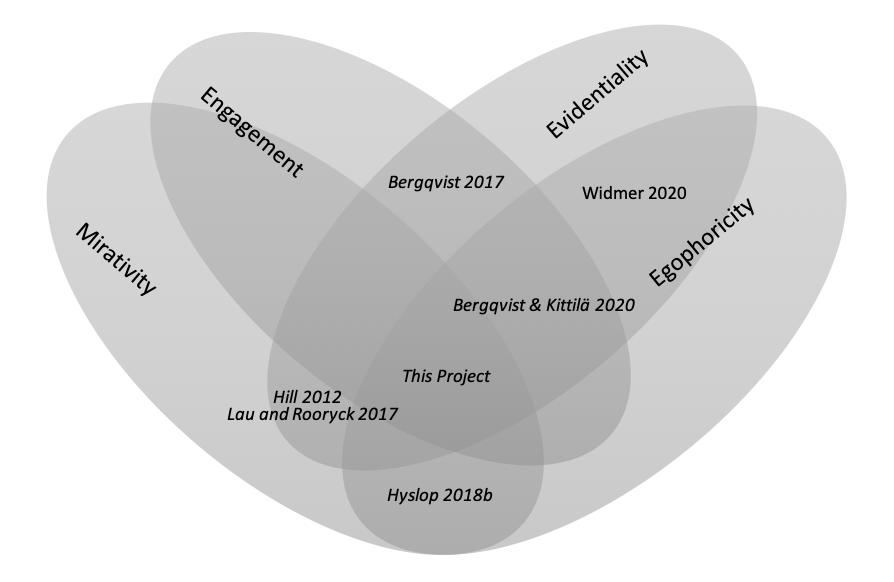
\includegraphics[width=\textwidth]{LitVenn.png}
    \caption{Examples of publications examining the crossovers between phenomena}
    \label{f:Conclusion:LitVenn}
\end{figure}

The functional motivations presented in Section \ref{s:Discussion:Motivations}, that of establishing shared ground between speech act participants, support the alignment of this field of epistemic marking with research into spatial reference and demonstratives such as in \citeA{GonzalezPerez2023}. Here, epistemics appear to fit into a larger set of deictic functional domains which factor physical and cognitive proximity to coordinate attention, awareness, and knowledge between speakers \cite{Peeters2016}. This relationship between epistemics and demonstratives has, of course already been observed in relation to engagement in \citeA{EvansBergqvistSanRoque2018a}, but given a shared functional motivation across all epistemic marking, can be seen to exist more broadly.

The primary conclusion of this work, that of the validity and relevance of an epistemic supercategory, can provide a foundation for the discussion and analysis of this marking moving forward, in relation to \lfam\ languages if not further afield. A number of case studies have already been presented in Chapter \ref{c:Discussion} where such a foundation improves or clarifies analysis of data that cannot readily be accounted for if a more siloed approach to the categorisation of forms and functions is used. These were, specifically, the mixed systems of Kurtöp (East Bodish: Bhutan) and Eastern Geshiza (rGyalrongic: PRC), and the socially conditioned epistemic systems of Ladakhi (Tibetic: India), Amdo Tibetan (Tibetic: PRC) and Milang (Siangic: India). In addition to these cases, there are well documented discussion in the literature about how to analyse mixed systems which were not specifically presented here as case studies, in particular regarding the three epistemic bases of Lhasa Tibetan \cite{DeLancey2017Tibetan}, the various epistemic bases of which have variously been described as solely evidential \cites{Garrett2001}{Gawne2017}, evidential and mirative \cites{DeLanceyMirativity1997}{DeLancey2012}, or egophoric and evidential \cites{Tournadre1992}{Widmer2017}. The analysis proposed here, of an epistemic supercategory in which each form sits on a gradient from strongest to weakest claim over epistemic authority and is conditioned in its usage by various deictic factors including source of evidence, confidence, and surprise, moves to unify these analyses. It argues that the specific differences between, for instance here, evidentiality and egophoricity as separate categories are not necessarily relevant here, but that a description of this system and many others across the \lfam\ family can be achieved without drawing these boundaries.

In addition to the primary conclusion of this work, that of the validity and relevance of an epistemic supercategory, a number of other typological observations were presented in \ref{c:Description} which could act as useful tools for the description and comparison of epistemic-marking systems across the \lfam\ family. In terms of the forms of these systems, a pattern relating to the size of systems was observed, splitting systems into single terms and complex systems, which could further be divided into reportative and other, and paradigmatic and scattered systems respectively. Another avenue for the categorisation of the data was seen in the position and scope of markings, in that they would appear as copulas, nominalisers, or as dedicated markers, the latter of which could take either verbal scope (attached to the verb) or clausal scope (e.g. sentence or clause final particles). In terms of functions, systems could be seen to either mark a single traditional category or multiple, though this distinction is less relevant when treating epistemic marking as a single coherent category, as has been argued in this thesis. It also noted patterns in the presence of explicit reference to addressee perspective (separate to any pragmatically necessary attention to the perspective of the addressee), which could occur on interrogatives, declaratives, both, or neither. 

Chapter \ref{c:History} began to use these typological observations, in particular the size of the systems in the dataset, to assess trends across the family in geographic terms. A comparison of these patterns with historical extra-linguistic factors across the Himalayas such as trade, religion, and political influence, then attempted to come to some conclusion about the origins and development of the widespread epistemic marking across the \lfam\ family. Here, it was able identify a trend for complex epistemic systems to occur mostly in regions with contact with Tibetic languages, while languages without epistemic marking at all tended to occur in contact with non-\lfam\ languages, or at least have a history of such. A lack of historical data on a number of key factors were shown to limit our ability at this stage to reconstruct the historical development of the marking in the family. These factors were historical levels of multilingualism, community sizes, and the time scale of the development of these systems (in turn obscured by a lack of shared forms between systems). Without these, we are unable determine whether the trends seen today are the result of areal diffusion of complex epistemic marking facilitated by the Tibetic family and its spread and influence across the Himalayas, or if instead epistemic marking is an inherited trait across the family that has been lost in languages with high levels of contact with non-\lfam\ languages. Regardless of the strength of the conclusions able to be drawn in this particular scenario, the investigation acts as an example of the typological observations presented in this theses in use, showing the insights that can be gained in its use.

\section{Limitations}
The framework proposed here is not being proposed as a replacement of all previous frameworks for the analysis of epistemic-marking systems in \lfam\ languages. Rather, it serves as a supplementary framework to both account for and describe systems where previous analytical frameworks have struggled to account for all variation, and compare forms and functions cross-linguistically where such comparisons would not otherwise be readily possible.

In particular, this thesis dealt with limited data in the sense that many \lfam\ languages were not considered. While efforts were taken to ensure as representative a sample as possible, discussed in detail in Section \ref{s:Methods:Collection}, the total number of languages that it was possible to sample was ultimately only a small percentage of the total diversity within the family. This is primarily a result of two factors. Firstly, there is necessarily a limit on the scope this project can take given the time restraints of a doctoral thesis. Secondly, in many areas of the family, descriptive data at the level of detail necessary for this project simply does not exist, or at least was not readily accessible to me online. The primary risk from this limitation is the possibility that a language with some incredibly divergent system of representing epistemic meaning and function has been missed, though presumably such a system, if it has been described as such in the literature, would have been salient enough in the literature to have been considered in the survey even if not included in the representative sample. For instance, languages such as Lhasa Tibetan and Ladakhi were not featured in the initial systematic survey, but were identified for their well researched and interesting epistemic systems nonetheless. Given this, if some such system which would drastically change the analysis presented in this thesis does exist in the family, it seems more likely that it simply has not yet been described. This does not, of couse, remove this limitation, but rather speaks to the value of further research on the typology epistemic marking even within the \lfam\ family.

Similarly, I am hesistant throughout my arguments to extend the conclusions here to language at a wider scale. In only surveying a single, albeit very large, language family, the arguments presented here can be well justified within the family but not beyond. Literature on languages outside the \lfam\ family does seem to follow general trends seen here. For instance, the marking evidential paradigm in Duna (Trans-New-Guinea: Papua New Guinea) marks the self as a source of evidence \cite{SanRoque2012}, representing the functional overlap between evidentiality and egophoricity both argued here and in previous literature on \lfam\ languages \cites{Gawne2017}{Hill2020}. Similarly, the attestation of engagement, marking speaker and addressee access to information is widespread and non limited to any one family or region \cite{EvansBergqvistSanRoque2018a}. Here again is an opportunity for further research, considering more widely how the categories of epistemic modality, evidentiality, egophoricity, mirativity, and engagement overlap and interact in terms of epistemic authority and the establishment of shared ground between speech act participants.

A more methodologically centred limitation of this research is the reliance on publically available analyses. The data is only as detailed as its description within the source material, which is not necessarily focussed on epistemic marking. It is difficult, if not impossible, to draw a line between descriptions where no there is no grammatically marked epistemic marking or where it has simply not been covered where it is never mentioned or clarified. This is particularly the case in shorter works such as grammar sketches (e.g. the historical language Pyu \cite[Subfamily Unclear: Myanmar][]{Miyake2019}), masters theses (e.g. Kayah Monu \cite[Karenic: Myanmar][]{Aung2013}), or some shorter doctoral theses (e.g. Zeme \cite[Zeme subfamily: India][]{Chanu2017}). Without specific mention of a lack of epistemic marking in any form, it is not really possible in these shorter descriptions to claim that epistemic marking is not present. In many ways, this stems from the wider issue regarding a lack of description across the family, rather than any specific limitation of the use of only publically accessible description.

\section{Further research}
As is the case with most, if not all research into \lfam\ languages, particularly in typology, there is an eternal need for wider reaching and more detailed descriptive coverage. This need is particularly strong, not just in the study of epistemics, with languages of unclear relationships to the wider family such as those in Bhutan (e.g. Lhokpu, Gongduk, Black Mountain Mönpa) and Arunachal Pradesh (e.g. Hruso, Milang, among others). Further documentary and descriptive work across the family will provide both further data to refine the conclusions drawn in this thesis, as well as an opportunity to test the descriptive and classificatory tools proposed here. There is also substantial scope, as discussed in terms of the limitations above, for the expansion of the conclusions established here to languages further afield. Research on the functional domains discussed in this thesis is prominent in areas such as South America (see the research of Karolina Grzech and Henrik Bergqvist, inter alia), and remains to be integrated into the framework presented here.

Beyond the constant call for broader and more detailed data, there remain some unanswered questions. Most of this thesis has focussed on epistemic marking limited to those with verbal or clausal scope. It only briefly in Section \ref{s:Discussion:Motivations} compared these systems to those with nominal or demonstrative scope. These epistemically conditioned nominal markers have been attested specifically with reference to engagement both within the \lfam\ family \cite{GonzalezPerez2022} and more widely \cites{EvansBergqvistSanRoque2018a}{EvansBergqvistSanRoque2018b}. It remains to be investigated in detail within this broader framework of epistemic marking how these (entirely or alongside spatial) epistemically conditioned forms relate to the verbal marking presented in this thesis, beyond an initial observation that there appear to be similarities in their underlying functional motivation. This thesis also largely limited its scope to grammatical marking in \lfam\ languages, avoiding lexical or periphrastic strategies of encoding epistemic meanings. As is touched on in Chapter \ref{c:Discussion}, the underlying pragmatics of epistemic marking are presumably shared across grammatical and other methods of encoding these meanings, and can presumably then to some extent be compared in functional (though not formal) terms. There is as such scope to consider the functions of these other epistemic-marking strategies in terms of the conclusions drawn here, especially in more isolating languages where the boundary between particle and lexeme might be harder to distinguish.
\appendix
\chapter{Field work and original data collection}\label{s:Methods:FieldMethods}
\section{Lhokpu}
During this project was collected first-hand data on Lhokpu (Subgroup unclear: Bhutan) to fill in a gap in the available data. As has been discussed above, Lhokpu has been potentially aligned with the Dimalish subfamily, and while the conclusions in \citeA{Grollmann2018} are certainly well supported, they have not necessarily been totally proven. As such, Lhokpu has been included in this study as an internal isolate of unclear subfamily per \citeA{VanDriem2014}.

Lhokpu is spoken in a small number of villages in the Dophuchen and Tading gewogs of Samtse District, in south-western Bhutan. There are two non-contiguous groups of speakers, one located about 15km up the Amo Chhu (River) from the other, which is in turn a similar distance upriver of Totopara, the village in which the potentially closely related language Toto is spoken. \citeA{Grollmann2018} estimate approximately 2500 speakers across all villages, though more recent estimates (Mareike Wulff, p.c. 2024) are as low as 800, many (potentially all) of whom also speak Nepali, and to a lesser extent, Dzongkha and English.

For this project, the data collected needed to efficiently reflect any epistemic-marking system that might exist in the language, as time in the field was strictly limited. With the time available (especially given this was a smaller component of the larger project), recording large amounts of natural and unprovoked dialogue, stories, and other content, and then identifying the relevant forms therein was not feasible. It can also be difficult to establish what the actual epistemic content of forms used in these settings would be, as it may not be totally clear to a researcher what the relationships of the speaker and addressee are to any given piece of information. On the other hand, it has been noted that speakers are not typically consciously aware of epistemic distinctions in language, and as such it can be difficult to ask or directly elicit them \cites{Gawne2013}{Grzech2020}. As such, as middle ground approach was used here, in which elicitation activities were used to generate naturalistic conversation data within an established and controlled epistemic context. These activities in particular draw from the work of \citesA{Gawne2013}{Gawne2020} and her discussion on using such tools, as well as \citeA{Grzech2020}.

\section{Field Methods and Elicitation Activities}
By establishing a set of contrastive epistemic contexts across the elicitation activities run, it is possible to, at least to a certain extent, ascertain more clearly the conditioning factors behind the selection of forms. The two primary activities that were run were the ``Family Problems Picture Task'' \cite{SanRoque2012a} and the ``Man and Tree Picture Sets'' \cite{Levinson1992}. These activities comprised the majority of the field work undertaken, and were supplemented by a small amount of elicitation of basic language structures and the collection of a wordlist.

\subsection{Family Problems Picture Task}\label{p:Methods:FamilyProblems}
The Family Problems Picture Task was specifically developed with the elicitation of epistemic forms in mind \cite{SanRoque2012a}, and involves four parts. First, two participants are presented with a set of images \cite{Carroll2009} depicting various interactions between family members in a pseudo-random order\footnote{the order is random for the participants, but is given by \citeA{SanRoque2012a} to allow for consistency and easier analysis down the line, so analysts do not need to work out which image is being described.} and are asked to describe them. Next, they are asked to confer and place the images in an order that depicts a story, and finally are asked to tell the story, once in third-person and once in first-person.

Across these parts, a number of different epistemic contexts are created. Table \ref{t:Methods:FamilyProblemsEvidentials} shows the these contexts, and the parts in which they are present. Visual evidence can be for information can be found in the descriptions and discussion, as participants are seeing the images for the first time, and subsequently discussing their contents. Similarly, inferential evidence could also be found in both, though potentially more prominently in the discussion phase, as participants are piecing together a story from the illustrations, requiring them to draw inferences about the exact events depicted. The description phase also shows equal epistemic authority over the images for both participants, as neither one will have seen the activity before. This equal authority might also be reflected as shared information, new information (i.e. mirative), or non-origo authority. Non-origo authority is distinguished from equal authority in that while they both accurately describe the epistemic context created in the task, equal authority refers to systems encoding that both speech act participants have the same authority, but not the strength of that authority, whereas non-origo authority refers to systems encoding specifically the lack of authority over the information at hand of the origo (speaker in declarative, addressee in interrogative), but does not directly reflect the addressee's perspective. Participatory evidence, or egophoric evidence \cite[][see ]{Gawne2017}, could be marked in the first-person telling of the story, as could, potentially along with the other parts, factual or neutral evidence as per \citeA{Zemp2020}.

\begin{table}\caption{Epistemic contexts covered by each part of the Family Problems Picture Task}\label{t:Methods:FamilyProblemsEvidentials}
       \noindent\adjustbox{center}{\begin{tabular}{r|c|c|c|c}
                                                  & Description & Discussion & Third-person telling & First-person telling \\
                     Visual evidence              & ✔           & ✔          &                      &                      \\
                     Inferential evidence         & ✔           & ✔          &                      &                      \\
                     Non-origo or equal authority & ✔           &            &                      &                      \\
                     Participatory evidence       &             &            &                      & ✔                    \\
                     Factual or neutral evidence  &             &            & ✔                    &
              \end{tabular}}
       
\end{table}


In some cases, namely with the non-origo and equal authority, as well as the participatory and factual evidentials, the conditions for two of the given epistemic bases are met in a single part of the activity. That is to say that, for instance, participatory evidence and factual evidence could theoretically be triggered by the same epistemic context. They are, however, functionally distinct in theoretical terms and as such have been included separately. That being said, without further evidence or usage contexts that are able to distinguish, it would not be directly possible from the data produced by this activity alone to determine if a given form used in the first-person telling, as an example, is conditioned by direct speaker involvement in the form of participatory evidence, or by a broader higher origo-authority as seen in factual evidentials. The typology of these similar-yet-different epistemic bases is discussed in greater detail in Section \ref{ss:Description:ClassByFunction}.

\subsection{Man and Tree Picture Sets}
The Man and Tree Picture Sets \cite{Levinson1992} are a series of image sets depicting plastic figures in various arrangements. Within the sets, different images show different arrangements of the same objects. Three sets were used in this project, some of which were combinations or subsets of the sets initially given in \citeA{Levinson1992}, and as such are given their own labels in the context of this project. The first set, \textsc{balls}, has four images showing red and yellow balls in various spatial and colour configurations. The second, \textsc{sawdust}, depicts a small pot full of sawdust, a plant, and a basket, with the pot variously covered, uncovered, overflowing, or entirely absent. The last set, \textsc{pigs}, shows a number of men, pigs, and small bushes in various numbers and configurations. The first two sets are substantially smaller than the {pigs}, and were used to teach participants the activity, and as a sort of warm-up activity.

The activity itself was run as a guessing game or director-matcher task, in which one participant, the matcher, has all images in the set laid out in front of them on cards, and the other, the director, has all images in a deck face-down. Between the participants is a partition such that the director cannot see the matcher's face-up array of images. One by one, the director draws a card and describes it to the matcher, who asks questions in turn, until the matcher is able to select which card the director has just drawn. They confirm that the card is correct, then repeat the process until all cards have been drawn.

The activity was originally designed for the elicitation of spatial reference systems, for which it was very effective here (though the analysis stemming from this falls outside the scope of this thesis), but has been repurposed here with a degree of success for the elicitation of epistemics. As with the Family Problems Picture Task, the activity creates a number of different epistemic contexts, though with the simpler task with fewer stages, there are fewer epistemic contrasts developed.

The Man and Tree activity has fewer separate stages than the Family Problems activity, and has been presented in Table \ref{t:Methods:ManTreeEvidentials} divided into the speech acts of each participant. The Director Description refers to the initial description of the image, and subsequent further comments on the image in response to questions from the matcher, which comprise the other speech acts in the activity. Visual evidence can be seen primarily in the initial descriptions of the images from the director. In all cases, however, this task shows unequal epistemic authority (contrasted with the Family Problems activity), in that the director has sole access to the aforementioned visual evidence at all times, and the matcher is either polling that visual evidence in asking questions, or polling a more authoritative evidence in confirming if they have selected the correct image. The useful difference between these two uses of unequal epistemic authority (the director and the matcher) then, is that one is speaker-origo, with the speaker referencing their own awareness, and the other is, being interrogative, likely addressee-origo.

\begin{table}
       \caption{Epistemic contexts covered by different areas of the Man and Tree Picture Task}\label{t:Methods:ManTreeEvidentials}
       \begin{tabular}{r|c|c}
                                          & Director Description & Matcher Questions \\
              Visual Evidence             & ✔                    &                   \\
              Unequal epistemic authority & ✔                    & ✔                 \\
              Shifted Origo in Questions  &                      & ✔
       \end{tabular}
       
\end{table}

The contrast between the equal epistemic authority in the Family Problems activity and the unequal epistemic authority here is a further distinction that is potentially able to be drawn from these two tasks. In other cases, it was these confirmation questions polling clearly non-shared unequal knowledge that was able to shed light on an epistemic system potentially conditioned by epistemic authority \cite{Bodnaruk2023}. In this case in particular, however, speakers did not verbally confirm their image choices. It is not clear if this is a fault of how the task was explained, if it was a result of the social dynamics between the participants, or just unfortunate chance.

\section{Outcomes}
These activities benefit from a solid foundation of analysis on the language such that individual forms can be better identified and separated after the activities are transcribed and translated \cite{Bodnaruk2023}. The lack of this foundation was a hindrance to the full analysis of the data gained, however, it was still possible to confirm some epistemic distinctions that had been originally attested in the basic elicitation. Transcriptions and translations were produced primarily in the field in \citeA{ELAN} together with local consultants, with some additional material being transcribed over WhatsApp after the conclusion of the field trip. \exref{e:Methods:LhokpuDistinction} shows the main epistemic contrast with a confident analysis from the elicitation activities.

\begin{exe}
       \ex\label{e:Methods:LhokpuDistinction}
       \begin{xlist}
              \ex\label{e:Methods:LhokpuDistinction:mi1}
              \gll nosam rang-ka [ganmo \textbf{mi}] \\
              mind \textsc{pron-gen} [wife \textbf{\textsc{cop.exist}}] \\
              \glt `In his mind, “My wife is there”.' (Family Problems)

              \ex \label{e:Methods:LhokpuDistinction:mi2}
              \gll ka-lok dzeʔ nih-pu \textbf{mi} \\
              \textsc{1.sg-obl} dog two-\textsc{clf.gen} \textbf{\textsc{cop.exist}} \\
              \glt `I have two dogs.' (Elicited)

              \ex \label{e:Methods:LhokpuDistinction:miha1}
              \gll kona i-du meʔ \textbf{mihã} \\
              then \textsc{prox-loc} fire \textbf{\textsc{cop.exist.evd}} \\
              \glt `Then here there is fire' (Man and Tree - Sawdust)

              \ex \label{e:Methods:LhokpuDistinction:miha2}
              \gll kanka it-dra \textbf{mihã} \\
              old.man one-\textsc{clf.anim}  \textbf{\textsc{cop.exist.evd}} \\
              \glt `There is one old man.' (Family Problems)\footnote{Speakers explained the use of the classifiers \textit{-dra} and \textit{-pu} as marking human and general referents, however the `human' classifier \textit{-dra} was occasionally used to refer to animals in the Man and Tree activity, along with the general classifier \textit{-pu}. No further classifiers have been identified yet.}
       \end{xlist}
       (Lhokpu)
\end{exe}

The form \textit{mi} is used as an existential copula in cases referring specifically to personal knowledge or experience, seen in \exref{e:Methods:LhokpuDistinction:mi1} where it reflects the personal insights of the character, and in \exref{e:Methods:LhokpuDistinction:mi2} where it reflects the privileged access of the speaker to information about themself. The alternative form \textit{mihã} is used in cases with direct visual evidence, in both \exref{e:Methods:LhokpuDistinction:miha1} and \exref{e:Methods:LhokpuDistinction:miha2} reflecting the speaker seeing parts of the images for the first time. Without further research, however, it is difficult to say exactly which of the contrastive aspects of the two epistemic contexts is responsible for the difference in forms. In any case, it is clear that there is a binary epistemic distinction on Lhokpu existential copulas, and that it is generally speaking a distinction between higher vs lower authority, with higher authority in the data occurring from personal insights or participatory/ego evidence, and lower authority from visual evidence.

Less confident conclusions were also able to be tentatively drawn regarding epistemic marking in verbal morphology. A limited understanding of some areas of the phonology of Lhokpu limited the analysis that was able to be undertaken here. A verb suffix \textit{-ah} occurs throughout the data collected in the elicitation activities, but not in any directly elicited data. Notably, the directly elicited data, sentences that were translated directly from English or Dzongkha into Lhokpu by consultants, are devoid of epistemic context. While, of course, such context can be described or imagined, the challenges in consious awareness of the conditions on the usage of epistemic forms as discussed above mean that these described situations are not reliable indicators of the actual usage of epistemic markers. The suffix \textit{-ah} is potentially equivalent to a form \textit{-a(l)} given by \cite{Grollmann2018}, with the lateral coda (dropped word finally) debuccalised, mirroring a sound difference between the data collected in Jigme village in this project and Grollmann and Gerber's (2018) data, wherein Grollmann and Gerber's possessive pronoun suffix \textit{-ŋa} is attested in Jigme as \textit{-ha}.\footnote{It is also possible from more recent data collection by Gwendolyn Hyslop, Mareike Wulff, and myself that this suffix is actually \textit{-ŋ̊a}, analysed differently due to the lack of in-depth documentation undertaken in both cases.} It is this glottal coda that is particularly challenging in the analysis of the form, as its phonological behaviour is not yet clear. While it is certainly present in many words, and its presence appears to be contrastive, it is not yet clear if another attested verb suffix \textit{-a} is a separate morpheme or an allomorph of \textit{-ah} with the glottal coda deleted. It is also possible that the glottal coda is present but remains undetected in the analysis. It is here that the lacking foundational knowledge of phonology and basic verbal morphology on the language seriously begins to hinder the analysis that can be completed at this stage.

\cite[20-21]{Grollmann2018} describe \textit{-a(l)} as marking something ``not personally experienced by the speaker or as not belonging to the personal knowledge of the speaker'', though do not provide examples. This functional description appears, at least at this stage, to work with the data collected here.

\begin{exe}
\ex \label{e:Methods:LhokpuVerbal}
\begin{xlist}

\ex \label{e:Methods:LhokpuVerbal:coda}
\gll ŋan dokm̥eŋ-su dzoŋ-do-\textbf{ah} \\
person walking.stick-\textsc{com} stand-\textsc{prog-\textbf{evd?}} \\
\glt `The person is standing with the stick.'

\ex \label{e:Methods:LhokpuVerbal:nocoda}
\gll siŋ-hõ hut-a dzoŋ-do-\textbf{a} le~le \\
tree-\textsc{towards} look-? \textsc{asp-prog-\textbf{evd?}} downhill~\textsc{adv} \\
\glt `Looking downhill towards a tree.' \\
(Man and Tree - Pigs)


\end{xlist}

\end{exe}

\begin{exe}
\ex \label{e:Methods:LhokpuVerbal2}
\begin{xlist}

\ex \label{e:Methods:LhokpuVerbal:cold}
\gll ka tɕuŋ̊-do \\
\textsc{1.sg} be.cold-\textsc{prog} \\
\glt `I am cold.'

\ex \label{e:Methods:LhokpuVerbal:cold2s}
\gll * na tɕuŋ̊-do \\
{} \textsc{2.sg} be.cold-\textsc{prog} \\
\glt *`You are cold.'

\ex \label{e:Methods:LhokpuVerbal:coldevid2}
\gll na ném-do-\textbf{ah} \\
\textsc{2.sg} be.cold.to.touch-\textsc{prog-\textbf{evd?}} \\
\glt `You are cold (to the touch).' \\


\ex \label{e:Methods:LhokpuVerbal:coldevid}
\gll tɕo ném-do-\textbf{ah} \\
water be.cold.to.touch-\textsc{prog-\textbf{evd?}} \\
\glt `The water is cold.' \\

\end{xlist}
(Elicitation) \\ 
Lhokpu (Subfamily Unclear: Bhutan)
\end{exe}


\exref{e:Methods:LhokpuVerbal} shows both \textit{-ah} and an occurrence of \textit{-a} that appears particularly likely to be an allomorph of \textit{-ah}, in both cases reflecting new, direct visual evidence, that was not previously part of the speaker's integrated knowledge. Much like with \textit{mi} and \textit{mihã}, it is difficult to say if, as suggested by \citeA{Grollmann2018} for \textit{-a(l)}, the use of \textit{-ah} is conditioned by the speaker's prior knowledge of some state of affairs, or if it is conditioned by the visual evidence the speaker has for their knowledge of that state of affairs. Notably, earlier in \exref{e:Methods:LhokpuVerbal:nocoda}, another instance of \textit{-a} is attested, at first glance here appearing to be a non-final marker connecting the verb \textit{hut} `look' with the finite-marked verb \textit{dzong} `sit', here marking an aspectual distinction. This non-final marker analysis does not seem to work for the emphasised marker, however, suggesting that, in lieu of an analysis that can account for both uses here, there are two functions or meanings for the suffix \textit{-a}, perhaps one of which is an allomorph of \textit{-ah}. \exrefs{e:Methods:LhokpuVerbal:cold}{e:Methods:LhokpuVerbal:coldevid} show a contrast between the use or lack of the \textit{-ah} suffix. It is not used in \exref{e:Methods:LhokpuVerbal:cold}, in which the speaker is referring to their internal experience using the verb \textit{tɕuŋ̊}, which is restricted to this meaning, seen by the rejection of \exref{e:Methods:LhokpuVerbal:cold2s}. In \exref{e:Methods:LhokpuVerbal:coldevid} and \exref{e:Methods:LhokpuVerbal:coldevid2}, however, the speaker is referring to an external observation and does use the (probable) evidential \textit{-ah} with the verb \textit{ném}, which specifically refers to temperature of other objects or individuals assessed through touch.

Between these two domains in which a probable epistemic distinction has been observed, this is the total extent of the current analysis into epistemic marking in Lhokpu, and as such is the total data that can be included. As is the case with published descriptive material, it is difficult to distinguish confidently between a language lacking a certain functional contrast, and such a contrast simply not being described in the current analysis. As such, when reading wider literature, conclusions cannot readily be drawn about systems lacking features. This limitation extends to the data collected for Lhokpu, simply because the analysis is nowhere near complete enough to confidently exclude any features. Instead, it is possible to preliminarily describe the system as occurring across multiple domains of the language, and containing a number of contrastive forms, conditioned by the closeness of the origo to the information. This closeness may depend on evidence source (direct visual vs general knowledge), participation or direct involvement, or some higher level claim of authority, though it is not yet clear if any single of these conditions is the sole relevant condition, or if it is in fact some combination thereof, or perhaps an entirely different condition.


\chapter{Table of Languages}\label{a:TableOfLanguages}
\begin{table}

\end{table}
\begin{longtable}[c]{ r c c }\caption{Languages surveyed in representative sample as discussed in Section \ref{s:Methods:Schema}. Subfamilies with no data available are also listed, marked with †. In cases where no data is available \textit{and} there are multiple languages in the subfamily, no language is given either.}
       \label{t:Appendix:LanguageReferences} \\
       Language           & Subfamily       & Source \\                                
       \hline \hline \endfirsthead 
       \caption{continued...} \\
       Language           & Subfamily       & Source \\                                
       \hline \hline \endhead 
       Tenyidie           & Angami-Pochuri  & \citeA{Kuolie2006}                     \\
       \hline
       Poumai Naga        & Angami-Pochuri  & \citeA{Veikho2021}                     \\
       \hline
       Jejara             & Ao              & \citeA{Barkman2014}                    \\
       \hline
       Mongsen Ao         & Ao              & \citeA{Coupe2007}                      \\
       \hline
       Bai                & Bai             & \citeA{Wiersma1990}                    \\
       \hline
       Mönpa              & Black Mountain  & \citesA{vanDriem1995}{Hyslop2016}      \\
       \hline
       Hakhun Tangsa      & Brahmaputran    & \citeA{Boro2017}                       \\
       \hline
       Garo               & Brahmaputran    & \citeA{Burling2003}                    \\
       \hline
       Atong              & Brahmaputran    & \citeA{Breugel2014}                    \\
       \hline
       Chepang            & Chepangic       & \citeA{Caughley1982}                   \\
       \hline
       Bhujel             & Chepangic       & \citeA{Regmi2007}                      \\
       \hline
       Idu                & Digarish        & \citeA{Blench2019}                     \\
       \hline
       Toto               & Dimalish        & \citeA{Basumatary2016}                 \\
       \hline
       Dhimali            & Dimalish        & \citeA{King2009}                       \\
       \hline
       Dura               & Dura            & \citeA{Schorer2016}                    \\
       \hline
       Kurtöp             & East Bodish     & \citesA{Hyslop2017}{Hyslop2018}        \\
       \hline
       Tawang Monpa       & East Bodish     & \citeA{Tombleson2020}                  \\
       \hline
       Lizu               & Ersuish         & \citeA{Chirkova2008}                   \\
       \hline
       Ersu               & Ersuish         & \citeA{Zhang2013}                      \\
       \hline
       Gongduk            & Gongduk         & NA\textsuperscript{†}                  \\
       \hline
       NA                 & Hrusish         & NA\textsuperscript{†}                  \\
       \hline
       Turung             & Kachinic        & \citeA{Morey2010}                      \\
       \hline
       Kadu               & Kachinic        & \citeA{Sangdong2012}                   \\
       \hline
       Karbi              & Karbi           & \citeA{Konnerth2020}                   \\
       \hline
       Kayah Monu         & Karenic         & \citeA{Aung2013}                       \\
       \hline
       Eastern Kayah      & Karenic         & \citeA{Solnit1986}                     \\
       \hline
       Duhumbi            & Kho-Bwa         & \citeA{Bodt2020}                       \\
       \hline
       Puroik             & Kho-Bwa         & \citeA{Lieberherr2017}                 \\
       \hline
       Chhathare Limbu    & Kiranti         & \citeA{Borchers2008}                   \\
       \hline
       Yakkha             & Kiranti         & \citeA{Schackow2015}                   \\
       \hline
       Daai Chin          & Kukish          & \citeA{SoHartmann2009}                 \\
       \hline
       Hyow               & Kukish          & \citeA{Zakaria2018}                    \\
       \hline
       Lepcha             & Lepcha          & \citeA{Plaisier2007}                   \\
       \hline
       Lhokpu             & Lhokpu          & Own Data                               \\
       \hline
       Nuosu (Sichuan Yi) & Ngwi-Burmese    & \citeA{Gerner2013}                     \\
       \hline
       Burmese            & Ngwi-Burmese    & \citeA{Soe1999}                        \\
       \hline
       Khatso             & Ngwi-Burmese    & \citeA{Donlay2019}                     \\
       \hline
       Magar              & Magaric         & \citeA{GrunowHarsta2008}               \\
       \hline
       Kham               & Magaric         & \citeA{Watters2002}                    \\
       \hline
       Meithei            & Meithei         & \citeA{Chelliah1997}                   \\
       \hline
       NA                 & Midzuish        & NA\textsuperscript{†}                  \\
       \hline
       Hkongso            & Mru             & \citeA{Wright2009}                     \\
       \hline
       Yongning Na        & Naic            & \citeA{Lidz2010}                       \\
       \hline
       Namuzi             & Naic            & \citeA{Pavlik2017}                     \\
       \hline
       Dolakha Newar      & Newaric         & \citeA{Genetti2007}                    \\
       \hline
       Kathmandu Newar    & Newaric         & \citesA{HaleNewar1980}{Hargreaves2017} \\
       \hline
       Trung              & Nungish         & \citeA{Perlin2020}                     \\
       \hline
       Anong              & Nungish         & \citeA{Sun2009}                        \\
       \hline
       Pyu                & Pyu             & NA\textsuperscript{†}                  \\
       \hline
       Munya              & Qiangic         & \citeA{Bai2019}                        \\
       \hline
       Qiang              & Qiangic         & \citeA{LaPolla2003}                    \\
       \hline
       NA                 & Raji-Raute      & NA\textsuperscript{†}                  \\
       \hline
       Eastern Geshiza    & rGyalrongic     & \citeA{Honkasalo2019}                  \\
       \hline
       Khroskyabs         & rGyalrongic     & \citesA{TaylorAdams2020}{Lai2017}      \\
       \hline
       Milang             & Siangic         & \citeA{Modi2017}                       \\
       \hline
       Southern Min       & Sinitic         & \citeA{Chen2020}                       \\
       \hline
       Tamang             & Tamangic        & \citeA{OwenSmith2014}                  \\
       \hline
       Western Tamang     & Tamangic        & \citeA{Regmi2018}                      \\
       \hline
       Maring             & Tangkhul        & \citeA{Kanshouwa2016}                  \\
       \hline
       Galo               & Tani            & \citeA{Post2007}                       \\
       \hline
       Tangam             & Tani            & \citeA{Post2017a}                      \\
       \hline
       Hile Sherpa        & Tibetic         & \citeA{Graves2007}                     \\
       \hline
       Amdo Tibetan       & Tibetic         & \citeA{Tribur2019}                     \\
       \hline
       Tshangla           & Tshangla        & \citesA{Andvik2010}{Grollmann2020}     \\
       \hline
       Tujia              & Tujia           & \citeA{Brassett2006}                   \\
       \hline
       Chhitkul-Rakchham  & West Himalayish & \citeA{Martinez2021}                   \\
       \hline
       Bunan              & West Himalayish & \citeA{Widmer2014}                     \\
       \hline
       Zeme               & Zeme            & \citeA{Chanu2017}                      \\
       \hline
       Inpui              & Zeme            & \citeA{Devi2014}                       \\
       \hline
\end{longtable}

\chapter{Static Database}\label{a:StaticDatabase}
Explain table and abbreviation key here
This sections presents a static and limited version of the database introduced in \cref{c:Methods}. It is included here for the sake of completeness in the submission of this thesis. A full and more accessible version of the database (and one that will continue to be updated) is available at \url{https://cbodnaruk.com/database/}.

Due to the size of the database and challenges in formatting it to fit in print, a number of column headings have been shortened, with a legend provided in Table \ref{t:Appendix:DatabaseLegend}
\begin{table}
       \centering
       \caption{Legend for the abbreviated headers in the printed static database given in Table \ref{t:Appendix:StaticDatabase}}\label{t:Appendix:DatabaseLegend}
       \begin{tabular}{r|l}
              Abbreviation & Meaning \\
              \hline
              A & Language Metadata \\
              \hline 
              B & Evidence of Epistemic Marking \\
              \hline 
              C1 & Verb Morphology \\
              C2 & Noun Phrase \\
              C3 & Verb Phrase \\
              C4 & Discourse Particle/Speech Act Scope \\
              \hline 
              D & Functions of Marking: Canonical \\
              EM & Epistemic Modality \\
              Ev & Evidentiality \\
              Ego & Egophoricity \\
              Eng & Engagement \\
              Mir & Mirative \\
              Oth & Other \\
              \hline 
              E & Functions of Marking: Non-Canonical \\
              \hline 
              F & Term(s) Used in Source \\
              \hline 
              G & Addressee Perspective \\
              G1 & Interrogative Structures \\
              G2 & Declarative Structures \\
              \hline 
              H & Other Features \\
              H1 & Diachronic Source (if given) \\
              H2 & Obligatory (if given) \\
              H3 & Mixed Paradigm \\
              H4 & Nominal Engagement \\ \hline
       \end{tabular}
\end{table} 
% Please add the following required packages to your document preamble:
% \usepackage{multirow}
% \usepackage[normalem]{ulem}
% \useunder{\uline}{\ul}{}
\begin{landscape}
       \begin{tiny}
       \begin{longtable}{p{1.2cm}p{1cm}|p{0.2cm}|p{0.2cm}p{0.2cm}p{0.2cm}p{0.2cm}|p{0.2cm}p{0.2cm}p{0.2cm}p{0.2cm}p{0.2cm}p{0.2cm}|p{0.2cm}p{0.2cm}p{0.2cm}p{0.2cm}p{0.2cm}|>{\raggedright\arraybackslash}p{2cm}|>{\raggedright\arraybackslash}p{1.5cm}>{\raggedright\arraybackslash}p{1.5cm}|>{\raggedright\arraybackslash}p{1.5cm}p{0.2cm}p{0.2cm}p{0.2cm}}

              \caption{A static version of the database introduced in \cref{c:Methods} and otherwise available at \url{https://cbodnaruk.com/database/}\label{t:Appendix:StaticDatabase}}\\
              \multicolumn{2}{l|}{A: Language Metadata} & B & \multicolumn{4}{l|}{C: Scope and Form} & \multicolumn{6}{l|}{D: Functions: Canonical} & \multicolumn{5}{l|}{E: Functions: Non-Can} & F & \multicolumn{2}{l|}{G: Addr} & \multicolumn{4}{l}{H: Other} \\
Language & Subfamily & & C1 & C2 & C3 & C4 & EM & Ev & Ego & Eng & Mir & Oth & EM & Ev & Ego & Eng & Mir &  & G1 & G2 & H1 & H2 & H3 & H4 \\ \hline \endfirsthead

\caption{continued}\\
Language & Subfamily  & B & C1 & C2 & C3 & C4 & EM & Ev & Ego & Eng & Mir & Oth & EM & Ev & Ego & Eng & Mir & F & G1 & G2 & H1 & H2 & H3 & H4 \\ \hline \endhead

Poumai Naga & Angami-Pochuri & + &  & + &  & + &  & + &  &  &  &  &  &  &  & + & + & evidential {[}277{]}, particle {[}333,336{]} (marking maybe mirative) & ? & + {[}138{]} demonstrative engagement &  &  & + & + \\
Tenyidie & Angami-Pochuri & -? &  &  &  &  &  &  &  &  &  &  &  &  &  &  &  &  &  &  &  &  &  &  \\
Jejara & Ao & + &  &  &  & + &  & + &  &  &  &  & + &  &  &  & + & Reportative, Mirative, Epsitemic Modal {[}144{]} & / & / & / &  &  &  \\
Mongsen Ao & Ao & - &  &  &  &  &  &  &  &  &  &  &  &  &  &  &  &  &  &  &  &  &  &  \\
Bai & Bai & - &  &  &  &  &  &  &  &  &  &  &  &  &  &  &  &  &  &  &  &  &  &  \\
Mönpa & Black Mountain & + & + &  &  &  &  &  &  &  & + &  &  &  &  &  &  & Evidential & / & / & / &  &  &  \\
Atong & Brahmaputran & + &  &  & + &  &  & + &  &  & + &  &  &  &  &  &  & Mirative {[}425{]}, Quotative {[}408{]} & / & + {[}426{]} narrative mirative & quotative from 'say' &  &  &  \\
Garo & Brahmaputran & + & + &  &  &  &  &  &  &  &  &  &  & + &  &  & + & "Terminal Suffix", descriptions but no terms & / & + counterexpective? {[}161{]} & / &  &  &  \\
Hakhun Tangsa & Brahmaputran & + &  &  &  & + &  & + &  &  &  &  &  &  &  &  &  & Reportative, Hearsay {[}352{]} & / & / & hearsay particle from 'to say'{[}352{]} &  &  &  \\
Bhujel & Chepangic & + &  & + & + &  & + &  &  &  &  & + &  & + &  &  & + & Mirative, Evidential & / & / &  &  &  &  \\
Chepang & Chepangic & + &  &  & + &  &  &  &  &  &  & + &  &  & + & + &  & Givenness, Information Flow & + {[}86{]} &  &  &  &  &  \\
Idu & Digarish & + &  &  &  & + &  &  &  &  &  &  & + & + &  &  &  & Evidential & ? & ? & ? &  &  &  \\
Dhimali & Dimalish & + &  &  &  & + &  &  &  &  &  &  & + & + &  &  & + & Deductive, Dubiative, Mirative & / & / &  &  &  &  \\
Toto & Dimalish & + & + &  &  &  & + &  &  &  &  &  &  &  &  &  &  & single Probability morpheme & ? & ? &  &  &  &  \\
Dura & Dura & + &  &  & + &  &  &  &  &  & + & + & + &  &  &  &  & Mirative, Presumptive (EM) & / & / & Mirative descended from nominalisation {[}233{]} &  &  &  \\
Kurtöp & East Bodish & + & + &  & + &  &  &  &  &  &  & + &  & + & + & + & + & Egophoricity and Mirativity, inference, dubiative and others {[}2018:115,134{]} & + & +? {[}2018: 125{]} & See Hyslop 2020 &  & + &  \\
Tawang Monpa & East Bodish & + &  &  & + &  &  &  &  &  & + & + &  & + & + &  &  & Perosnal,Testimonial,Neutral & + & / & / &  & + &  \\
Ersu & Ersuish & + &  &  &  & + &  & + &  &  &  & + &  &  &  & + &  & Direct, Inferred, Reportative & + & +? {[}2013:547 counterexpective q tag{]} &  &  &  &  \\
Lizu & Ersuish & + & + &  &  &  &  & + &  &  &  & + & + &  & + &  &  & First-hand, inferential, quotative; egophoric & + & / & Some details on reportative from "say", cognate in Ersu & Yes? &  &  \\
Gongduk & Gongduk & NA &  &  &  &  &  &  &  &  &  &  &  &  &  &  &  &  &  &  &  &  &  &  \\
Sajolang & Hrusish & + & + &  &  & + & + &  &  &  &  & + &  & + &  &  & + & Mirative, Evidential, Dubiative, Emphatic &  & + & dir evidential from "do", assumption from "seem" &  &  &  \\
Kadu & Kachinic & + &  &  &  & + & + &  &  &  &  &  &  & + &  &  & + & Hearsay, Mirative & ? & ? Mirative {[}404{]} &  &  &  &  \\
Turung & Kachinic & +? &  &  &  & + &  &  &  &  &  &  & + & + &  & + &  & Reportative Evidential {[}458{]}, epistemic meanings of imperatives {[}455-6{]} & / & / &  & No &  &  \\
Karbi & Karbi & + &  &  &  & + & + & + &  &  &  &  &  &  &  &  &  & Quotative, Reportative, Dubiative &  & + &  &  &  &  \\
Eastern Kayah & Karenic & + &  &  & + &  &  &  &  &  &  &  &  & + &  &  &  & quotative &  & / & verb to say &  &  &  \\
Kayah Monu & Karenic & - &  &  &  &  &  &  &  &  &  &  &  &  &  &  &  &  &  &  &  &  &  &  \\
Duhumbi & Kho-Bwa & + & + & +? &  &  &  & + &  &  &  & + &  &  &  &  & + & Evidentiality & /? & + {[}408,413{]} & Various are given in ch.8 &  &  &  \\
Puroik & Kho-Bwa & + &  &  & + &  &  & + &  &  &  &  &  &  &  &  &  & Quotative &  &  & Grammaticalised from 'say' &  &  &  \\
Chhathare Limbu & Kiranti & + &  &  &  & + &  &  &  &  &  & + &  & + &  &  & + & Descriptions given with no terms {[}2007{]} & / & / & As with Yakkha, borrowed from Nepali &  &  &  \\
Yakkha & Kiranti & + &  &  & + & + &  &  &  &  & + & + & + & + &  &  &  & Mirative, reportative, probability {[}516{]} &  & + & Mirative borrowed from Nepali &  &  &  \\
Sunwar & Kiranti & -? &  &  &  &  &  &  &  &  &  &  &  &  &  &  &  &  &  &  &  & Yes &  &  \\
Daai Chin & Kukish & + & + &  &  & + &  & + &  &  & + &  &  &  &  &  &  & Mirative, Evidential & ? & /? &  &  &  &  \\
Hyow & Kukish & + &  &  &  & + &  &  &  &  &  & + &  & + &  &  & + & Surprise, Unpredicted & ? & + {[}437{]} surprising marker marks general surprise &  &  &  &  \\
Lepcha & Lepcha & + &  &  & + &  &  &  &  &  &  & + &  &  &  &  & + & Dubiative, Possibility, inferential, certainty, discovery particles & / & + {[}136,165{]} & Predominantly forms of extant full verbs &  &  &  \\
Lhokpu & Lhokpu & + & + &  & + &  &  & + &  &  &  &  &  &  &  &  &  &  & + &  &  & Yes &  &  \\
Burmese & Lolo-Burmese & -? &  &  &  &  &  &  &  &  &  &  &  &  &  &  &  &  &  &  &  & Yes &  &  \\
Nuosu (Sichuan Yi) & Lolo-Burmese & + &  &  &  & + &  &  &  &  &  & + &  & + &  &  &  & Quotative only {[}377{]} & / & / & Grammaticalised from 'say' in proto-Yi & No? &  &  \\
Kham & Magaric & + &  &  & + & + & + &  &  &  & + & + &  & + &  &  &  & Mirative, Counterexpective, Reportative, Possibility, Probability & + two forms of questions based on expected response & + {[}291{]} mirative requires fact of discovery to be relevant to listener & Possibly grammaticalised from 'say' &  &  &  \\
Magar & Magaric & + & + &  &  & + & + &  &  &  &  & + &  & + &  &  & + & Mirative, Direct/Factual. Reportative, Inferred & + & +? {[}486-487, c reads a bit like IS{]} &  &  & + &  \\
Meithei & Meithei & + & + &  & + &  &  & + &  &  &  & + &  &  &  & + &  & Numerous; indirect evidence {[}211{]}, attitude enclitics {[}250{]}, more on {[}295{]} & + {[}295{]} & + & / & No &  &  \\
 & Midzuish & NA &  &  &  &  &  &  &  &  &  &  &  &  &  &  &  &  &  &  &  &  &  &  \\
Hkongso & Mru & + &  &  &  & + &  &  &  &  &  & + & + &  &  &  & + & Mirative, Dubiative, Speaker Oriented Modalities & / & / &  & No &  &  \\
Namuzi & Naic & +? &  &  &  & + &  &  &  &  &  &  & + &  &  &  & + & "surprise or assurance" {[}150{]} & ? & ? &  &  &  &  \\
Yongning Na & Naic & + &  &  & + &  &  & + &  &  &  &  & + & + &  &  &  & Common Sense, Evidentiality {[}476{]} & ? & ? &  & No & + &  \\
Dolakha Newar & Newaric & - &  &  &  &  &  &  &  &  &  &  &  &  &  &  &  &  &  &  &  &  &  &  \\
Kathmandu Newar & Newaric & + & + &  &  & + &  &  & + &  &  & + &  & + &  &  &  & Conjunct/Disjunct {[}Hargrave: 458{]}, Quotative {[}464{]} and some other clause particles {[}465{]} & + & / & / &  &  &  \\
Khatso & Ngwi-Burmese & + &  &  &  & + &  &  &  &  &  & + & + &  &  & + &  & Strong Assertion Marker, Epistemic Emphatic Particle &  & + {[}440-441{]} &  & No &  &  \\
Anong & Nungish & - &  &  &  &  &  &  &  &  &  &  &  &  &  &  &  &  &  &  &  &  &  &  \\
Trung & Nungish & + &  &  & + & + &  &  &  &  &  & + &  & + &  &  & + & Mirative, Evidential & /? & /? & Some from verbs &  & + &  \\
Pyu & Pyu & NA &  &  &  &  &  &  &  &  &  &  &  &  &  &  &  &  &  &  &  &  &  &  \\
Munya & Qiangic & + &  &  & + & + & + & + & + &  &  &  &  & + &  & + & + & Egophoric, Mirative, Evidential & / & / & Functionally very similar to Lhasa Tibetan &  & + &  \\
Qiang & Qiangic & + & + &  &  &  &  & + &  &  & + &  & + &  &  &  &  & Direct, Inferential/Mirative, Hearsay & + {[}207{]} & / & hearsay particle from 'to say'{[}204{]} &  & + &  \\
 & Raji-Raute & NA &  &  &  &  &  &  &  &  &  &  &  &  &  &  &  &  &  &  &  &  &  &  \\
Eastern Geshiza & rGyalrongic & + & + &  &  & + & + & + &  &  &  & + &  & + & + & + &  & Evidential, Mirative, Non-Shared Information, more terms therein {[}582{]}, Epistemic Certainty {[}575{]} & + & + & Some, various sources given for each form in chapter 9 &  & + &  \\
Khroskyabs & rGyalrongic & + &  &  &  &  &  &  &  &  &  &  &  & + &  &  & + &  &  &  &  &  & + &  \\
Milang & Siangic & + &  &  & + &  &  &  & + &  &  &  & + & + &  &  &  & Egophoric {[}455{]}, reportative, uncertain & + & ? & Lexical verbs {[}460{]} & Yes &  &  \\
Southern Min & Sinitic & -? &  &  &  &  &  &  &  &  &  &  & + &  &  &  &  & Adverbs/Modal Verbs & / & / &  &  &  &  \\
Tamang & Tamangic & + & + &  &  & + &  & + &  &  & + &  & + &  &  &  &  & Mirative, Evidentiality & + & ? &  & Yes & + &  \\
Western Tamang & Tamangic & + & + &  &  &  &  &  &  &  & + &  &  &  &  &  &  & Mirative & / & / &  &  &  &  \\
Maring & Tangkhul & + & + &  &  &  &  & + &  &  &  &  & + &  &  &  & + & Evidential, Mirative,   Direct &  &  &  &  &  &  \\
Galo & Tani & + & + &  & + &  &  &  & + &  &  & + &  &  &  &  &  & Conjunct/Disjunct {[}607{]}, Various Clause Final Particles {[}625{]} & + {[}607{]} & +? {[}634,639{]} & Some only (Uncertainty from irrealis marker) &  &  &  \\
Tangam & Tani & + &  &  &  & + &  &  &  &  &  & + & + & + &  &  & + & Hearsay, Counterexpective & ? & +? {[}73{]} counterexpective &  & No & + &  \\
Amdo Tibetan & Tibetic & + & + &  & + &  &  & + & + &  &  & + &  & + & + &  & + & Egophoricity & + {[}453{]} & ? &  &  &  &  \\
Hile Sherpa & Tibetic & + & + &  & + &  &  & +? & + &  &  & + &  & + & + &  & + & Mirative, Past-Observational, Observational, Disjunct,   Volitional & + {[}222{]} & / & / &  &  &  \\
Tshangla & Tshangla & + & + &  & + &  &  &  &  &  &  &  & +? & + & + &  & + & Subjective (Bjokapakha) {[}232{]}, Mirative (Standard) {[}227{]}, hearsay & + Grollman grammar {[}232{]} & / & Grollman 2020b & Yes & + &  \\
Tujia & Tujia & - &  &  &  &  &  &  &  &  &  &  &  &  &  &  &  &  &  &  &  &  &  &  \\
Bunan & West Himalayish & + & + &  &  &  &  & + & + &  &  &  &  &  &  &  &  &  &  & + {[}2014:503{]} conjuct portrays addressee as volitional & Ego/non-ego in present, tibetic evidentials in past & No & + &  \\
Chhitkul-Rakchham & West Himalayish & + &  &  & + &  & + & + &  &  &  &  &  &  &  &  & + & Perceptual, Dubiative, Assertive, Pers Experience, Pers Assertive & + {[}172{]} & + &  &  & + &  \\
Inpui & Zeme & - &  &  &  &  &  &  &  &  &  &  &  &  &  &  &  &  &  &  &  &  &  &  \\
Zeme & Zeme & - &  &  &  &  &  &  &  &  &  &  &  &  &  &  &  &  &  &  &  &  &  & 
       \end{longtable}
\end{tiny}
\end{landscape}
\printbibliography
\end{document}
